% !TeX program = xelatex
% (C) Hans Wan, Windy Deng
% Licensed under CC BY-NC-SA 4.0 International license.
% This is the LaTeX source code of Your Missing Semester of Using Computer (PDF Version).

\documentclass[a4paper]{book}
\usepackage{missing}

\date{\today}

\begin{document}

\pagenumbering{Alph}
\maketitle

\frontmatter
\pdfbookmark{内封}{innertitle}
\thispagestyle{empty}
\begin{center}
  \vspace*{1.5cm}
  \fontsize{42pt}{54pt}\selectfont{}\textsf{你缺失的那门}\par
  \fontsize{18pt}{18pt}\selectfont{}\textsf{Your Missing Semester of Using Computer}\par
  \fontsize{54pt}{8pt}\selectfont{}\textbf{\textsf{计算机课}}\par
  \vspace*{2.6cm}
\end{center}

\begin{note}
  我们十分期望得到读者的建议和意见:无论是对编写方向有好的建议,还是发现了叙述不正确或不严谨的地方,亦或是找到了一个错别字,都请加群向我们反馈或将反馈发送到邮箱 \href{mailto:missing@criwits.top}{\texttt{missing@criwits.top}} 哦!
\end{note}

这是一份适合电脑小白入门的电脑使用课程。它平易近人,娓娓道来,介绍了从基本的文件管理,到软件的寻找安装,再到各类使用技巧与优良软件推荐的许多内容,旨在帮助读者在信息化时代更灵活地使用电脑。

这也是一份面向今日与未来的信息时代指南。它立足当下,探索变革,讲述了当今热门的生成式 AI、网络安全、物联网与云计算等前沿技术的概念、原理和应用,能够引导读者立于数字化时代的潮头,把握科技发展的方向。

零门槛、易理解、有深度,与时俱进、开放共享——这是《你缺失的那门计算机课》不断追求的目标,也是我们努力的方向。

\begin{center}
  \vspace*{1cm}
  \begin{minipage}{.45\textwidth}
    \centering
    \vskip0.6cm
    \includegraphics[width=3.8cm]{assets/QR_code.pdf}\par
    \vskip0.6cm
    访问 \url{https://www.criwits.top/missing}\par
    或扫码阅读本书最新版本!\par
  \end{minipage}
  \qquad
  \begin{minipage}{.45\textwidth}
    \centering
    \vskip0.6cm
    \includegraphics[width=3.8cm]{assets/QQ_group.pdf}\par
    \vskip0.6cm
    扫码或搜索群号858831033\par
    加入《你缺计课》交流群!\par
  \end{minipage}
\end{center}  

\setcounter{premepi}{1}
\chapter{序}
\label{premble}

按理来说,对于所谓「Z 世代」的年轻人,熟练地使用电脑应该是他们的生活必备技能。

但事实却并非如此。据我们观察,许多同学对电脑的使用也并不熟悉,甚至可以说是陌生:
他们可能在网上被下载到各种「P2P 高速下载器」,面对着满电脑的流氓软件而不知所措;
他们可能对着别人发来的 \texttt{zip} 或 \texttt{7z} 文件一头雾水,对「压缩」和「解压缩」都不甚熟悉;
他们可能装着四五个浏览器、三四个杀毒软件,更可能分不清自己电脑的「内存」和「硬盘」……

这或许是由于智能手机的普及造成的。
显然,使用电脑与使用手机相比,「复杂」了不止一个数量级。
然而,尽管几年前就有人说「电脑现在已经是夕阳产业了」,但事实却是:
至少在当下,我们仍然得学会去用电脑,不说多么「精通」,但至少要能知道「软件怎么找怎么装」「出现小问题怎么办」「XX 文件怎么打开」「怎么把文件打包」等等这些「21 世纪的常识」。

中小学的《信息技术》课堂、大学的《大学计算机基础》课程本应起到教授这些知识的作用。
可惜,事与愿违——很多时候,我们在这些课堂上学到的东西,可能一辈子都用不到;真正需要学的东西,却缺失了:

我们一辈子可能也不会再尝试用 Excel 排出张三李四不及格的科目有哪些,不会再折腾复杂到毫无意义的页眉和页脚,不会再碰和动画制作和网页相关的任何内容。
但我们未来必然有无数次会需要去网上下载一个新的软件,会无数次遇到各种各样的软件错误、闪退或者崩溃,会无数次因为 Windows 更新导致这样或那样的问题,会无数次遇到电脑沾上垃圾软件而奇慢无比无法使用……

这份《Your Missing Semester of Using Computer》是一份为「电脑小白」准备的电脑操作指南。
它直译过来就是《你缺失的那门计算机课》,也可以叫做《你本应学过的计算机课》。
我们会假定读者基本不了解电脑的操作,换言之就是所谓「电脑小白」,告诉读者「电脑最好怎么用」。

这份教程会在文中简称自己为《Missing》。
《Missing》的得名参考了 MIT 的《\href{https://missing.csail.mit.edu/}{The Missing Semester of Your CS Education}》。

\tableofcontents

\mainmatter

\part{基础篇}[
  感谢你开始阅读《你缺计课》!现在展现在你面前的,是《你缺计课》的基础篇。在这一部分,我们将介绍那些虽然基础但十分重要的电脑基本操作,从认识我们电脑的每个组成部分开始,学习文件管理的方法,尝试安装、卸载各种软件,并掌握基本的电脑维护知识。
]
\addtocontents{toc}{\protect\footnotetext[2]{标有「*」的为选读内容}}

\setcounter{chapter}{-1}

\chapter{一些约定与预备知识}
\label{cha:first-things-first}

俗话说,「磨刀不误砍柴工」。在一切开始之前,我们先对本书中的一些标记和约定进行说明,同时为你提供一些可能有助于你更好地阅读本书的预备知识。

\section{《你缺计课》是什么}

《你缺计课》是一门\regcolor{面向当下的「零门槛」电脑课}:《你缺计课》旨在帮助你轻松掌握「如何在当下更高效地使用电脑」。如果你是电脑小白,本书会手把手地引导你迈入数字世界;如果你已经熟悉电脑操作,它也能助你发现可能忽略的小技巧,查漏补缺。

《你缺计课》是一本\regcolor{展望未来的「信息化」科普书}:从计算技术到人工智能,从云计算到网络安全,本书以通俗易懂的语言,带你探索这些塑造当今与未来的核心技术,让你对信息化世界有更清晰的认识。

\section{《你缺计课》不是什么}

《你缺计课》\regcolor{不是任何软件的使用手册}:本书不会详细讲解某款软件的具体操作方法。相反,我们更注重帮助你理解各种软件的功能、特点以及它们在不同场景中的作用。

《你缺计课》\regcolor{不是大部头而死板的教材}:有别于枯燥、繁琐而呆板的专业教材,本书希望和你成为朋友,与你一同踏上一场轻松愉快的旅程。它轻松、有趣、接地气,贴近生活,伴你前行。

\section{文中的标记符号}

在《你缺计课》中,我们使用方头括号「【】」来标记所有屏幕上字面显示的选项。例如,当我们希望你右键桌面上的图标
\begin{figure}[htb!]
  \centering
  \includegraphics[width=2cm]{assets/basic/This_PC.png}
\end{figure}

\noindent 时,我们会称「右键【此电脑】」。

我们使用右箭头「→」来表示下一步操作。例如,「右键【此电脑】→【属性】」的意思是,右键桌面上的【此电脑】图标,然后在弹出的菜单中点击【属性】。

如果某一章节的标题后带有星号「*」,表明这一章节内容可能较难理解,可以选择性阅读。

本书中的网页链接与邮箱地址会以这种样式呈现:\url{https://criwits.top/missing};一些代码片段、文件路径、特殊数字等内容会以 \MissingVerb{这种形式} 呈现。

\begin{note}
  有这种特殊外框的文字,通常是一些题外话。它们可能是一些供你思考的问题,或是一些有助于理解正文的额外知识。
\end{note}

\begin{MissingVerbatim}
这种特殊外框的文字是上述“代码片段”等内容的“升级版”,在内容太长,行内空间不足以展示时使用。这种环境对“行”很敏感,过长的一行文字会用换行标记标出,比如这行,看起来有三行,其实是一行。
这才是第二行。
\end{MissingVerbatim}

\section{快捷键的操作说明}

如果你按快捷键(组合键)后,电脑并没有行使预想的功能,可能是你的按法不对。快捷键的按法并不是「同时按下所有的键」,而是「依展示次序按下各键不松手,最后一起松开」。例如,若要按快捷键「\keys{\Windows + Shift + S}」:

\begin{itemize}
  \item 先按住 \keys{\Windows} 键(\keys{\Windows} 键上印有 Windows 徽标「\Windows」或「\WindowsTen」,一般来说这个键在 \keys{Ctrl} 和 \keys{Alt} 之间)不要松手;
  \item 再按住 \keys{Shift} 键,同样不要松手;
  \item 接着按一下 \keys{S} 键,然后松开全部按键。
\end{itemize}

\section{\keys{F1} -- \keys{F12} 功能键的使用说明}

在很久以前,人们为了增加电脑键盘的使用效率,在键盘的最顶端设计了一排按键,它们就是 \keys{F1} -- \keys{F12} 功能键。这些功能键和键盘上的 \keys{Ctrl}、\keys{Alt} 等键一样,并不能用来输入文字,而是用来组合出各种功能的。比如,\keys{Alt + F4} 可以用来关闭当前程序,\keys{F5} 可以用来刷新网页,\keys{F1} 用来查找帮助等。

随着电脑操作方式不断演进,\keys{F1} -- \keys{F12} 键使用得越来越少。这时,人们想,与其让这些键在键盘上吃灰,不如赋予它们一些新功能,比如快捷调整屏幕亮度、音量、无线网络连接等设置。于是,一些电脑键盘,尤其是笔记本电脑的键盘上,这 12 个按键在它们原本的功能之外,增加了一层「扩展功能」。

\begin{figure}[htb!]
  \centering
  \includegraphics[width=.9\textwidth]{assets/basic/F1_to_F12_keys_with_extra_functions.png}
  \caption{带有额外功能的 F1—F12 功能键}
  \label{fig:F1_to_F12_keys_with_extra_functions}
\end{figure}

上图展示的就是 \keys{F1} -- \keys{F12} 键拥有扩展功能的键盘。这里,\keys{F1} -- \keys{F12} 这些键上被画上了一些符号。这些符号代表了这些键的扩展功能。例如,上图中 \keys{F5} 键上画有亮度降低的符号,因此 \keys{F5} 键的扩展功能就是降低屏幕亮度; \keys{F1} 键画有静音的符号,因此 \keys{F1} 键的扩展功能就是静音。

为了让 \keys{F1} -- \keys{F12} 键能够在这两种功能中自如切换,人们在键盘左下角安排了一个 \keys{Fn} 键(意思是 function,功能)。具体地,对于一台具有 \keys{Fn} 键的电脑,它的键盘情况是下列两种情况中的一种:

\begin{enumerate}
  \item 直接按 \keys{F1} -- \keys{F12} 功能键可以行使它们原本的功能,按住 \keys{Fn} 的同时再按 \keys{F1} -- \keys{F12} 则行使它们的扩展功能。例如:按 \keys{F5} 可以在浏览器中刷新页面(常见浏览器基本都可以),按 \keys{Fn + F5} 可以降低屏幕亮度。
  \item 直接按 \keys{F1} -- \keys{F12} 功能键可以行使它们的扩展功能,按住 \keys{Fn} 的同时再按 \keys{F1} -- \keys{F12} 则行使它们原本的功能。例如:按 \keys{F5} 可以降低屏幕亮度,按 \keys{Fn + F5} 可以在浏览器中刷新页面。
\end{enumerate}

\begin{figure}[htb!]
  \centering
  \includegraphics[width=.8\textwidth]{assets/basic/Fn_functions.pdf}
  \caption{\keys{F1} -- \keys{F12} 的两种功能情况}
  \label{fig:Fn_functions}
\end{figure}

你可以随便打开一个应用(比如浏览器),然后按 \keys{Alt + F4}。如果刚打开的应用退出了,就说明你的电脑属于上面两种情况中的第一种。如果没有反应,就属于第二种。

有些键盘提供了快捷的方法在这两种模式中切换。比如某些笔记本电脑键盘,可以通过按 \keys{Fn + Esc} 来切换这两种模式。另一些键盘可能需要使用专门的软件来进行调整,具体还请参考你的笔记本电脑或者键盘的说明书。

\begin{note}
	这意味着,对于那些包含 \keys{F1} -- \keys{F12} 功能键的快捷键,如果你按下后电脑没有反应,不妨在按住 \keys{Fn} 的同时再试一次——你的键盘有可能是上面的情况 2,\keys{F1} -- \keys{F12} 功能键只有在按住 \keys{Fn} 时才发挥原本的作用。
\end{note}

\section{「重启」不是关机再开机}

对今天大多数的电脑来说,「重启」过程并不等价于「先关机再开机」的过程。若在我们在文中提及了「重启」操作,请务必选择开始菜单中的「重启」选项重启电脑,而非将电脑关机后再手动打开。

\section{存储容量的单位}

我们对本书中使用的容量单位「TB」「GB」「MB」「KB」的关系约定如下:
\[
  1\,\mathrm{TB}=1024\,\mathrm{GB}=1024\times1024\,\mathrm{MB}=1024^3\,\mathrm{KB}=1024^4\,\text{字节}
\]
我们有时会略去这些单位最后的字母「B」,即文中可能用「1 T」来表示「1 TB」。

\begin{note}
  如果你有买过 U 盘,你会发现标称「128 GB」的 U 盘实际可用的容量只有 119 GB 左右。这是因为生产 U 盘的厂家用「1000 进位」来计算容量,而我们使用的 Windows 操作系统则用「1024 进位」来计算容量。为了避免换算带来的麻烦,本书与操作系统的用法保持一致,使用「1024 进位」。
\end{note}

\section{「设置」和「控制面板」}

在今天的大多数电脑上,「设置」app 用于对系统绝大多数的选项进行调整。我们可以在开始菜单中找到一个齿轮图标的应用,点击它就可以打开「设置」。按键盘上的 \keys{\Windows + I} 也可以打开它。文中,「打开系统设置」的说法均是指打开这个应用。

\begin{figure}[htb!]
  \centering
  \includegraphics[width=.6\textwidth]{assets/basic/Settings.png}
  \caption{设置}
  \label{fig:Settings}
\end{figure}

你可能听说过「控制面板」这个词,它是 Windows 10 之前的 Windows 系统中用来调整系统设置的应用。在今天我们常用的 Windows 10 和 Windows 11 中,控制面板仍然存在,但它的功能已经被「设置」app 取代。只有当我们在文中明确使用「控制面板」一词时,才需要你使用它。

\practice

\begin{enumerate}
  \item 计算 1 GB 等于多少 KB?等于多少字节?假设一个汉字占两个字节,1 GB 大约可以记录多少个汉字?
  \item 尝试计算,一个按 1000 进位计算得到容量为 64 GB 的 U 盘,按 1024 进位计算得到的容量是多少?
  \item 在自己电脑上尝试这些快捷键:
    \begin{enumerate}
      \item \keys{\Windows + Shift + S} (仅限 Windows 10 / 11)
      \item \keys{Ctrl + Shift + Esc}
      \item \keys{\Windows + D}
    \end{enumerate}
  \item 如果你在用笔记本电脑,了解并体验它 \keys{F1} -- \keys{F12} 功能键的扩展功能。
\end{enumerate}
\chapter{认识你的电脑}
\label{cha:computer-and-its-components}

\begin{intro}
  或许电脑对你来说,是一个熟悉却又神秘的「黑箱」:它早已融入我们的生活,但我们却很少真正了解它的组成与结构。阅读完本章,你将找到这些问题的答案:

  \begin{itemize}
    \item 什么是「CPU」?别人说的「i5」「i7」都是什么?「双核」「四核」又是什么?
    \item 为什么说「内存」和「硬盘」不一样?存储东西的到底是内存还是硬盘?电脑特别卡,到底是内存不够还是硬盘不够?
    \item 我想玩游戏,选购电脑时应该关注什么方面?「显卡」是什么东西?
    \item 什么是「Windows」?那「Windows 11」又是什么?为什么苹果笔记本的系统界面看起来和我不一样?我用的是什么系统?
  \end{itemize}
\end{intro}

如今,电脑几乎「无所不能」,已经成为了我们生活和工作中不可或缺的一部分。每一台电脑内部,都充满了复杂的电子电路和元器件,它们是人类智慧的结晶,构成了电脑的「硬件」部分。而在这冷冰冰的硬件之上,「软件」赋予了电脑生命与功能——从办公、学习到娱乐,各种软件让我们的生活更加便捷。可以说,硬件如同电脑的「身体」,软件则是电脑的「思维」,它们共同构成了「电脑」这个有机体。

本章将引领你深入认识自己的电脑:从最基础的硬件开始,我们将逐一介绍它们的功能与作用,并分析这些硬件如何影响电脑的性能。接着,我们将了解运行在这些硬件之上的各种软件,介绍它们与硬件的协同和配合,让你对电脑的构成和运行有一个更加全面的了解。

\section{电脑内部的硬件} 

本节我们将介绍电脑内部的那些关键硬件。即使你并没有亲眼见过各种硬件模块的模样,但通过这一节的介绍,你也会对它们形成基本的了解。

在开始之前,我们先假设这样一个场景:某位老师收集了一个班的作业,现在需要批改它们,如下图所示。

\begin{figure}[htb!]
  \centering
  \includegraphics[width=.5\textwidth]{assets/basic/Teacher_and_homework.png}
  \caption{正在批改作业的老师}
  \label{fig:teacher-and-homework}
\end{figure}

我们可以把老师批改作业的过程分解成下面的步骤:

\begin{enumerate}
  \item 老师将这一摞作业堆在办公桌的一边,腾出办公桌的中央和另一边。
  \item 现在,老师取下这一摞作业中的一小叠,放在办公桌中央,开始伏案批改。
  \item 老师批改完了这一小叠作业,然后将它们放在办公桌的另一边,摞成新的一沓。
  \item 重复步骤 2 和步骤 3,最终老师完成了全部作业的批改,这时批改完的作业全部在办公桌的另一边。
\end{enumerate}

这个例子有什么用呢?请先记住它,它将帮助我们更好地理解电脑硬件的工作原理。

\subsection{处理器(CPU)}

中央处理器(Central Processing Unit),简称「处理器」,英文简写「CPU」,是电脑内部最重要的一枚芯片,可以想象成是电脑的「大脑」。在上面的例子中,老师就相当于电脑中的处理器:老师的作用是批改作业,从而完成教学任务;处理器的作用是进行各种运算,从而实现电脑不同的功能。

你一定注意到过,电脑会发热——热到需要用一个风扇给它降温,这热量中有很大一部分就是处理器发出来的。如果你有关注过时事和新闻,中美贸易战之中关键的一环,正是处理器芯片。下图中,左边是一枚台式机的 CPU,右边是一枚笔记本电脑的 CPU。

\begin{figure}[htb!]
  \centering
  \includegraphics[width=.6\textwidth]{assets/basic/Two_CPUs.pdf}
  \caption{常见的台式机和笔记本电脑的处理器芯片}
  \label{fig:Two_CPUs}
\end{figure}

\begin{note}
  你可能会疑惑:这两个 CPU 为什么看起来很不一样?这是因为笔记本 CPU 为了节省空间,会直接将 \underline{➋「晶片」}(芯片的核心部分,由硅制成)裸露在外;而台式机 CPU 为了保护晶片,会在其外罩上一层 \underline{➊ 金属盖}。
\end{note}

处理器是电脑工作的核心,因此,\regcolor{处理器的性能就很大程度上决定了电脑的性能,决定了我们使用这台电脑流不流畅、玩游戏卡不卡、工作效率高不高}。在今天,全世界电脑芯片基本上是由两家美国公司设计\footnote{事实上,芯片的「设计」和「制造」两件事是不一样的,就像能设计出房屋的建筑师不一定会到工地上去砌墙。英特尔能够自行完成从设计到制造整条生产链,而 AMD 只能完成设计,它的处理器是由专门负责制造芯片的厂商(例如台积电)生产的。}的,其中一家叫做「英特尔」(Intel),另一家叫做「AMD」。

\begin{itemize}
  \item 英特尔公司现在主要的 CPU 产品线称作「酷睿」(Core),而「酷睿」系列又分成了三个子系列,每个子系列都有不同档次的产品。
    \begin{table}[htb!]
      \centering
      \caption{英特尔CPU产品系列}
      \label{tab:Intel-CPUs}
      \begin{tblr}{
        colspec = XX[2]X[4]X[4],
        cells = {c, m},
        cell{Z}{2-Z} = {j},
        row{1} = {fg = white, bg = missing, font = \bfseries},
        row{even} = {MissingSkyBlue},
      }
        \toprule
        & 传统酷睿系列 & 酷睿 Ultra 系列 & 酷睿数字系列 \\
        \midrule
        低端 & 酷睿 i3 & 酷睿 Ultra 3 & 酷睿 3 \\
        中端 & 酷睿 i5 & 酷睿 Ultra 5 & 酷睿 5 \\
        高端 & 酷睿 i7 & 酷睿 Ultra 7 & 酷睿 7 \\
        顶尖 & 酷睿 i9 & 酷睿 Ultra 9 &  ---\footnotemark \\
        说明 & 传统的酷睿系列,自 2008 年起沿用至今 & 2023 年发布的新系列,主要应用在高端笔记本电脑产品上,增加了针对 AI 应用的优化 & 2024 年发布的新系列,针对笔记本电脑产品进行了能耗方面的优化 \\
        \bottomrule
      \end{tblr}
    \end{table}
    \footnotetext{截至 2024 年 12 月,英特尔并没有推出酷睿 9 系列的 CPU。}\\
    大多数使用英特尔 CPU 的电脑,机器表面会贴一个类似左下图的蓝色(或灰色、黑色)贴纸。对于笔记本电脑,通常贴在键盘下方或机器背面;而对于品牌台式机,则通常贴在机器正面、侧面或顶面,如右下图所示。
    \begin{figure}[htb!]
      \centering
      \includegraphics[width=.7\textwidth]{assets/basic/Intel_sticker.png}
      \caption{英特尔的贴纸}
      \label{fig:Intel_sticker}
    \end{figure}\\
    \begin{figure}[htb!]
      \centering
      \includegraphics[width=.6\textwidth]{assets/basic/AMD_sticker.png}
      \caption{AMD的贴纸}
      \label{fig:AMD_sticker}
    \end{figure}
  \item AMD 公司现在主要的 CPU 产品线称作「锐龙」(Ryzen),而锐龙系列也分成了 3 个档次——「R5」「R7」和「R9」\footnote{其实还有 R3,但是很少在消费市场见到。}。大多数使用 AMD CPU 的电脑会粘贴类似图 \ref{fig:AMD_sticker} 的橙黑或橙灰色贴纸。
\end{itemize}

\begin{note}
  除了英特尔和 AMD 之外,亦有一些厂商能够生产电脑的 CPU,例如苹果、高通,以及国产厂商龙芯、华为等。不过,这些厂商生产的 CPU 与英特尔、AMD 的 CPU 往往并不兼容,使用这些 CPU 的电脑需要使用专用的系统和软件。想了解更多有关这些 CPU 的细节?请阅读本书超越篇的\nameref{cha:program-and-arch}。
\end{note}

我们常常说一台电脑是「双核」「四核」的,这里的「双核」「四核」就是处理器中的概念。今天,几乎所有 CPU 都在芯片中安装了多个「核心」,相当于一个个协同起来的独立的小处理器。例如,「双核」意味着在一枚处理器芯片上集成了两个核心,相当于两个大脑协同工作,当我们需要用电脑同时做很多事情的时候就有所裨益。同理,「四核」「八核」就是在一个芯片上集成了四个甚至是八个核心。现在,一些 CPU 还使用「大小核」设计,混合使用大小两种规格不同的核心,来实现性能和功耗之间的平衡。下图中,左方是一枚四核 CPU 示意图,右方则是一枚采用大小核设计的六核处理器示意图(图片非实际比例)。

\begin{figure}[htb!]
  \centering
  \includegraphics[width=.6\textwidth]{assets/basic/Multicore.pdf}
  \caption{多核CPU示意}
  \label{fig:Multicore}
\end{figure}

然而,核心数只能反映「脑子多不多」,但无法刻画「一个脑子有多快」。要衡量一颗 CPU 的性能,除了直观地根据厂商划定的这些低中高端系列之外,「主频」也是一个重要的参考。所谓「主频」指的是这 CPU 一秒种能够「工作」的次数,人们通常使用单位「GHz」来标注它。1 GHz 就表示「1 秒能『工作』10 亿次」。CPU 通常有一个「基准频率」和「加速频率」,前者是 CPU 正常工作时的稳定频率,后者则是在短时间内应对复杂任务时能达到的最高频率。目前,常见的台式机 CPU 的基准频率和加速频率能达到 3 GHz 和 5 GHz,而笔记本则在 2 GHz 和 4 GHz 左右。

需要强调的是,\regcolor{并不是说核心数越多、主频越高的处理器性能一定越好},更\regcolor{不是说 i7 处理器就一定比 i5 更好},也\regcolor{不是说英特尔和 AMD 有孰优孰劣之分}。我们应该综合理解这些概念:每个品牌都会随着时间推移一代代地更新,每一代都有着的不同系列,有的系列高端,有的系列低端;每个系列也都有自己的不同型号,有的型号性能强,有的型号性能弱。CPU 的性能并不与某一个因素呈线性的关系,而是多个因素叠加的结果。

按 \keys{Ctrl + Shift + Esc} 打开「任务管理器」,选择【性能】页面,就能看见 CPU 的型号、基准频率(标注为【基准速度】)和核心数(标注为【内核】)。

\begin{note}
  你也可以右击【开始按钮】,选择【任务管理器】来打开「任务管理器」。
\end{note}

\begin{figure}[htb!]
  \centering
  \includegraphics[width=.65\textwidth]{assets/basic/Check_CPU.png}
  \caption{在任务管理器看看CPU}
  \label{fig:Check_CPU}
\end{figure}

\subsection{内存(RAM)}

紧接着,我们介绍能直接与处理器交流的部件——内存,英文简写「RAM」。上一小节提到,处理器相当于大脑,但与大脑不同的是,处理器只能\regcolor{处理}数据,而这些待处理的数据,需要依赖外部的元件来临时存放。内存就是用来临时存放数据的。

内存的核心组件是一个个黑色的「内存芯片」。目前,内存芯片的主要生产厂商集中在韩国和中国台湾。这些芯片通常被排列在条形电路板上,形成一个模块,方便插入电脑主板进行更换或升级。这样的整体被称为「内存条」。如下图所示,左侧展示的是台式电脑使用的内存条,而右侧则是笔记本电脑使用的版本。不过,\regcolor{为了节省内部空间,很多笔记本电脑选择将内存芯片直接焊接在主板上,这种设计的内存无法更换或升级}。

\begin{figure}[htb!]
  \centering
  \includegraphics[width=.7\textwidth]{assets/basic/RAMs.jpg}
  \caption{不同的内存条}
  \label{fig:RAMs}
\end{figure}

前文说,内存直接与处理器进行数据交流。与处理器那极快的运算速度相匹配,内存的读取与写入速度也是极快的。但内存有一个特点——\regcolor{断电即丢失数据}。也就是说,当你电脑关机,内存中的数据便不复存在,又回到白纸一块。这种特性决定着,内存只能用来在电脑工作时临时存储信息。

回到前面老师批改作业的场景。办公桌的中央区域可以理解为「内存」:老师将作业放在办公桌中央批改,是因为这里改起来最方便;处理器将数据放在内存中处理,是因为这里读取和写入速度最快。办公桌中央不能总是放着东西,不然会弄乱、弄丢;内存中的数据一旦断电就会消失,因此总是临时的。

在 21 世纪初,电脑内存的容量不大,有 512 MB 已经不得了了。但随着科技发展,现如今,大容量内存已经司空见惯。在今天,要想让一台电脑能基本流畅运行,内存容量应当至少有 8 GB。当然这东西倒是多多益善,就像更大的桌子能摆更多东西一样,\regcolor{更多的内存意味着更多的空间来让处理器存放数据,也就意味着电脑能同时处理更多的任务,基本意味着电脑更加流畅。}据我们的经验,在目前(2024 年),16 GB 的内存对于日常使用已经够用;但如果你有大型游戏、三维建模、大型软件开发等需求,选择 32 GB 乃至更大的内存会更加合适。

\begin{note}
  对应到手机中,内存有时会被手机厂商称为「运行内存」,不过我们不推荐如此称呼。原因请参见下面「硬盘」一节。
\end{note}

在任务管理器的【性能】页的【内存】一栏,你可以看见自己电脑的内存总量等信息。

\subsection{硬盘}

内存是用来临时存储数据的,而硬盘则是用来长久保存数据的。与内存相比,硬盘的读写速度要慢得多,但存在硬盘中的数据不会因为断电而轻易消失,因此,硬盘是数据的最初的起点和最终的归宿:处理器在一开始,从硬盘中取出数据放入内存,在内存中处理数据,处理完成之后,再将新的数据放回硬盘。

\begin{note}
  所以,你电脑的所有资料都存在硬盘里。想直接拿走你的资料,应该去拿硬盘,而不是拿走显示器或别的什么东西。
\end{note}

\regcolor{除了各种各样的数据——各种文档、图片、音乐——之外,电脑上各种各样的软件本身,也是存放在硬盘里面的。}相信你在手机上有过这样的经验——手机的「存储空间」不够用,除了删掉一些不需要的照片、视频外,卸载不常用的 app 也是一个快捷的办法。在电脑上,情况是一样的:卸载软件,释放的其实就是硬盘上的空间。

\begin{figure}[htb!]
  \centering
  \includegraphics[width=.7\textwidth]{assets/basic/HDD_and_SSD.png}
  \caption{常见的硬盘}
  \label{fig:HDD_and_SSD}
\end{figure}

在前面老师批改作业的场景当中,办公桌两侧堆作业的地方可以理解为「硬盘」:大量的作业被堆在那里,整齐摆放,不会弄散、弄丢,但老师总是要把作业取到趁手的地方(办公桌中央)来批改;大量的数据被存在硬盘里,不会因为断电就丢失,但处理器总是要把数据放在快速的地方(内存)来处理。

简单来说,硬盘现在分为两种,一种叫「机械硬盘」(Hard Disk Drive,简称「HDD」),如图 \ref{fig:HDD_and_SSD} 左侧所示,容量大、价格低、速度更慢,利用电磁原理存储数据。另一种叫「固态硬盘」(Solid State Drive,简称「SSD」),如图 \ref{fig:HDD_and_SSD} 右侧所示,容量小、价格高、速度较快(但远远没有内存那么快)。SSD 用芯片存储数据,但这种芯片和内存的那种不同,断电还能保持数据。不过,不管是哪种硬盘,如果硬盘许久不用(不给它通电),那里面的数据也会慢慢消失,固态硬盘大约是 3 至 5 年,而机械硬盘最多 20 年——所以,对于存了东西但没有装入电脑的备用硬盘,要定期拿出来通电运转一下。

在今天(2024 年),标称容量 1 TB 的固态硬盘大约 500 元,机械硬盘大约 300 元;标称容量 2 TB 的固态硬盘大约 800 元,机械硬盘大约 400 元。因此,有些电脑会用一块小容量(512 GB 及以下)的固态硬盘,搭配一块大容量(1 TB 及以上)的机械硬盘来实现各自功能的互补。但也有一些中高端电脑会直接选用一整块大容量(比如 1 TB 甚至 2 TB)的固态硬盘而不再使用机械硬盘。

\regcolor{一块硬盘的空间可以被划分成不同的「盘」(学名叫「分区」)来更好地使用}。双击桌面上的【此电脑】来打开「文件资源管理器」,你看到的「C 盘」「D 盘」就是各个分区。在下一章\nameref{cha:file-and-file-management},我们将向你介绍如何管理好自己硬盘上的东西。 

\begin{figure}[htb!]
  \centering
  \includegraphics[width=.8\textwidth]{assets/basic/Partitions.png}
  \caption{一些分区}
  \label{fig:partitions}
\end{figure}

\begin{note}
  如果你在桌面上没有看到【此电脑】图标,你也可以按下 \keys{\Windows + E} 组合键来打开文件资源管理器,然后在左侧的导航栏中找到【此电脑】。

  如果你想在桌面上显示【此电脑】图标,请先打开系统设置,然后选择【个性化】,找到【主题】。

  \begin{center}
    \includegraphics[width=.6\textwidth]{assets/basic/Open_personalization_in_settings.png}
    \captionof{figure}{找到【主题】设置}
    \label{fig:Open_personalization_in_settings}
  \end{center}

  然后,在界面下方找到【桌面图标设置】(Windows 10 可能显示在界面右方),勾选【计算机】(即【此电脑】),再点击【应用】。你也可以把其他几个常用的图标勾选上,比如【用户文件】、【回收站】等。

  \begin{center}
    \includegraphics[width=.6\textwidth]{assets/basic/Select_This_PC.png}
    \captionof{figure}{选择要显示的图标}
    \label{fig:Select_This_PC}
  \end{center}

  这样,你的桌面上就会显示那些对应的图标了。
\end{note}

\regcolor{硬盘对电脑使用体验的影响,主要是打开软件的速度,包括开机的速度。}这是很容易理解的,因为数据和软件本身原先都是存在硬盘里的,处理器从硬盘里取数据的速度就直接影响着软件启动或者说加载的时间。

\begin{note}
  手机中用类似固态硬盘一样的芯片来存储数据,有些手机厂商和商家会称之为「内置存储」「存储内存」甚至是「内存」,但它\regcolor{完全不是}内存。这是为什么有人会弄混内存和硬盘的根源之一。人们常说的「手机内存不够」,指的往往是存储空间(可以称「手机的硬盘」)不够,而不是真正的「内存不够」。
\end{note}

\begin{figure}[htb!]
  \centering
  \includegraphics[width=.65\textwidth]{assets/basic/Check_disk_status.png}
  \caption{在任务管理器看看硬盘}
  \label{fig:Check_disk_status}
\end{figure}

打开「任务管理器」,切换到【性能】选项卡,其中【磁盘 0】【磁盘 1】就是一块块硬盘,其后的括号内则列出了该硬盘上的分区。点击一块硬盘,可以看到它的大小和类型(机械硬盘 HDD、固态硬盘 SSD)等信息。

\subsection{显卡(GPU)}

如果你是喜欢玩游戏的读者,「显卡」将是你在选购电脑时需要着重考虑的一个因素。

以前,「显卡」就是电脑里面的一个独立的模块,像一张卡一样插接在主板上。这个模块的功能是专门进行画面的绘制和图像的处理,因而得名「显卡」。所有显示在屏幕上的画面,都是由显卡绘制的。因而,\regcolor{显卡的好坏对游戏和图形相关的工作(比如三维制图、视频编辑)有较大影响}。下图展示了一块老旧的电脑显卡,其中 ➊ 是用于连接显示器的端口,➋ 处则是与电脑主板连接的触点。➌ 为这块显卡的散热风扇,而在其下方压着的 ➍,就是显卡的核心部分——图形处理器(Graphics Processing Unit,简称 GPU)。

\begin{figure}[htb!]
  \centering
  \includegraphics[width=8cm]{assets/basic/GPU_parts.png}
  \caption{老显卡(也是现在显卡)的各部分}
  \label{fig:GPU_parts}
\end{figure}

\begin{note}
  也就是说,GPU 是一枚芯片,而显卡是承载着这个芯片的模块。不过现在,人们习惯于将这两个词混用——既可以用「GPU」代指整个显卡,也可以用「显卡」或「显卡芯片」一词来特指 GPU 那枚芯片。强求区分它们显得有点古板学究气了,因此在本书中,我们也会混合使用两种称呼。
\end{note}

为什么上面那段要加上「以前」两个字呢?因为随着半导体技术的发展,人们后来发现,GPU 可以「集成」到处理器\footnote{一开始,集成显卡并不是集成到处理器中的,而是集成在主板上的一个芯片之中(称为「北桥」),后来才集成到了处理器里面。}中,换言之,就像多核处理器把几个核心放在一个芯片上一样,GPU 也可以和 CPU 做成一块芯片。容易想到,这样集成到一起之后,受限于芯片整体的大小,GPU 不能做得性能很强了:CPU 就在它边上,与它一起发热,一起分享能量。但是,通过这种方式,可以有效缩小硬件的体积,也能降低功耗。因而,发展到今天,GPU 在电脑中的形态有了以下两种:

\begin{itemize}
  \item \regcolor{集成显卡},简称「\regcolor{集显}」,又称「\regcolor{核显}」,英特尔称「核芯显卡」,AMD 则将 GPU 和 CPU 构成的整体一同称为「APU」。GPU 被安排在处理器的同一片芯片上,性能相对较差,能应付大多数工作,但游戏、制图等特定工作就不太行了。集成显卡功耗很低,而且省去了用户单独购买显卡的麻烦。
  \item \regcolor{独立显卡},简称「\regcolor{独显}」。GPU 仍然是一片独立的芯片,以显卡模块的形式安装在电脑内。这样的 GPU 性能较强,但换来的是更高的功耗、更大的体积和更多的发热等。如果你喜欢玩游戏(尤其是大型 3D 游戏),又或者从事视频编辑、三维设计等工作,那么一台装有独立显卡的电脑可能是你的刚需。
\end{itemize}

今天,全世界生产\regcolor{独立显卡}的厂商主要有两家,一家叫「英伟达」(NVIDIA),它旗下的显卡俗称「N 卡」;另一家则是前文提到过的 AMD,它推出的显卡俗称「A 卡」。如果你有涉足过游戏交流圈,玩家所说的「RTX 4090」「GTX 1080 Ti」等都是英伟达显卡的型号,而「RX 6800 XT」「RX 580」等都是 AMD 显卡的型号。下图是英伟达网站上出售的\CJKsout*{《黑神话·悟空》联名款的} RTX 4070 Super 高端显卡,可以看到显卡上有三个大尺寸的散热风扇,这从侧面说明其功耗之大、发热之多。

\begin{figure}[htb!]
  \centering
  \includegraphics[width=.6\textwidth]{assets/basic/4070_storepage.png}
  \caption{在售的RTX 4070 Super}
  \label{fig:4070_storepage}
\end{figure}

\begin{note}
  除了英伟达和 AMD 之外,市面上也有一些其他品牌的独立显卡。或许来源于在集成显卡设计上的经验,英特尔也推出了自己的独立显卡系列。同时,我国公司「摩尔线程」也率先推出了面向民用市场的国产显卡,具有比较优秀的理论性能。然而,由于市面上的游戏、软件大都主要针对英伟达和 AMD 显卡进行设计、优化,摩尔线程显卡的实际体验目前还有许多的提升空间。
\end{note}

一般来说,对于笔记本电脑,轻薄本大都使用集成显卡,而游戏本大都装配有独立显卡。显然,这是由它们的使用场景和目标人群不同所决定的。不过,因为笔记本电脑内部空间相当有限,笔记本内即使装配了独立显卡,它们的性能也要比同级别的台式机独立显卡要差。同时,笔记本的独立显卡往往不是「插」而是「焊」在主板上的,我们几乎不可能对它们进行更换、升级,更别说给没有独立显卡的笔记本电脑加装一块独显\footnote{不过,如果你的笔记本电脑配有「雷电 3」「雷电 4」或「OCuLink」等接口,你可以通过这个接口连接外置的独立显卡来使用,但是这样做并不十分方便,受众并不多。}。

我们可以把 GPU 的任务理解成「根据 CPU 的命令,画出图形并输出到显示器上」。为了完成这个任务,\regcolor{GPU 拥有属于自己的内存,称为「显存」}。GPU 使用显存空间来暂时存放它正在绘制的画面,同时还要存放大量与图形有关的其他内容。这使得显存的大小成为了决定(独立)显卡性能和价格的一个重要因素。目前,高端的独立显卡拥有 10 GB 甚至 20 GB 以上的显存,这使得它们得以从容应对各种复杂的游戏画面。而至于集成显卡,它们则需要从电脑内存中「借」一部分空间充当显存,因此更难以应付大量的图形工作。

值得注意的是,近些年来,随着人工智能(AI)技术的发展,GPU 的功能已经不再局限于「打游戏」「制图」等图形工作——\regcolor{在 AI 模型的训练和推理过程中,GPU 的并行计算能力能提供比处理器更好的性能},同时独立显卡的显存还能提供比电脑内存更快的访问速度。如果你了解过 AI 绘画或 AI 作曲等技术,在它们的说明文档中,你一定会看到对 GPU 的需求。若你对这方面有兴趣,那么 GPU 的性能,尤其是显存的大小,就成了你选购电脑时的重要考虑因素。

\begin{note}
  想了解和 AI 有关的更多知识?没问题!请看超越篇的\nameref{cha:bring-intelligence-to-machines}。
\end{note}

在任务管理器中,我们同样可以看到有关显卡的信息:在【性能】页面左侧的列表末尾,【GPU 0】【GPU 1】等就表示着我们电脑上的一张张显卡。

\section{与我们「打交道」的软件}

\subsection{软件与操作系统}

由处理器、内存、硬盘以及各种各样的外围电子元件,共同构成了一台电脑的硬件部分。而在硬件之上,具体的工作任务是由软件来指派的。

我们可以用每天都在用的手机来理解:\regcolor{手机上,无论是我们自己安装的「QQ」「微信」「网易云音乐」,还是手机预置的「电话」「短信」,都属于「软件」}。「QQ」「微信」指挥硬件去利用网络收发信息,利用屏幕展示数据;「网易云音乐」指挥硬件去播放声音,同时在屏幕上展示评论;「电话」「短信」指挥硬件利用无线电模块发送和接收信号……同样一部手机,硬件还是那个硬件,但能通过不同的软件行使不同的具体功能。

而在「QQ」「微信」「电话」等 app 和纯粹的硬件之间,有\regcolor{一个更大,而且更「底层」的软件,称为「操作系统」}。简单地说,操作系统「夹」在各软件和硬件之间,为软件具体行使功能提供了一系列方便的「接口」。有了操作系统,网易云音乐 app 不再需要真正地去想「怎么让喇叭发声」,而只需要考虑「怎么告诉操作系统让喇叭发声」。「让喇叭发声」是一个带些复杂物理知识的过程,但「告诉操作系统让喇叭发声」则相对简单得多。

\begin{figure}[htb!]
  \centering
  \includegraphics[width=.8\textwidth]{assets/basic/OS_structure.pdf}
  \caption{App、操作系统和硬件的关系}
  \label{fig:OS_structure}
\end{figure}

\begin{note}
  尽管操作系统是一个特殊的软件,但在日常生活中,「软件」一词通常只指微信、QQ 或是 Word、PowerPoint 等「应用软件」,即 app。在本书中,除非特别说明,「软件」和「app」是相同的含义,我们会混合使用它们。
\end{note}

由于上层的软件需要依赖操作系统来实现功能,而每个操作系统留给软件的接口细节上也有所不同,因此,\regcolor{针对不同操作系统开发的软件是不能直接通用的}。软件厂商一般会为不同的操作系统开发同一款软件,这样就能照顾到使用不同系统的用户。

今天,主流的手机操作系统有「安卓」(Android)、「iOS」以及「鸿蒙」(Harmony OS)。安卓系统是开放的,因此被各个手机厂商广泛使用,而 iOS 和鸿蒙目前则分别用在苹果和华为的设备上。如果你在网上下载过手机 app,一定会注意到厂商要根据操作系统提供不同的下载入口,这正是因为不同系统上的软件相互不兼容。

而在电脑上,「Windows」「Linux」及「macOS」是最常见的三种操作系统。\regcolor{Windows 最为普遍,几乎所有的个人电脑都运行着 Windows 系统}。Linux 是一种开源的操作系统,主要在服务器上使用,一些专业人士也会在日常使用;macOS 则是苹果推出的电脑操作系统,理论上只能用于苹果的电脑。下图中,(a) 至 (c) 依次是 Windows 11、Linux(使用 GNOME 桌面环境)和 macOS Sonoma 的界面。

\begin{figure}[htb!]
  \centering
  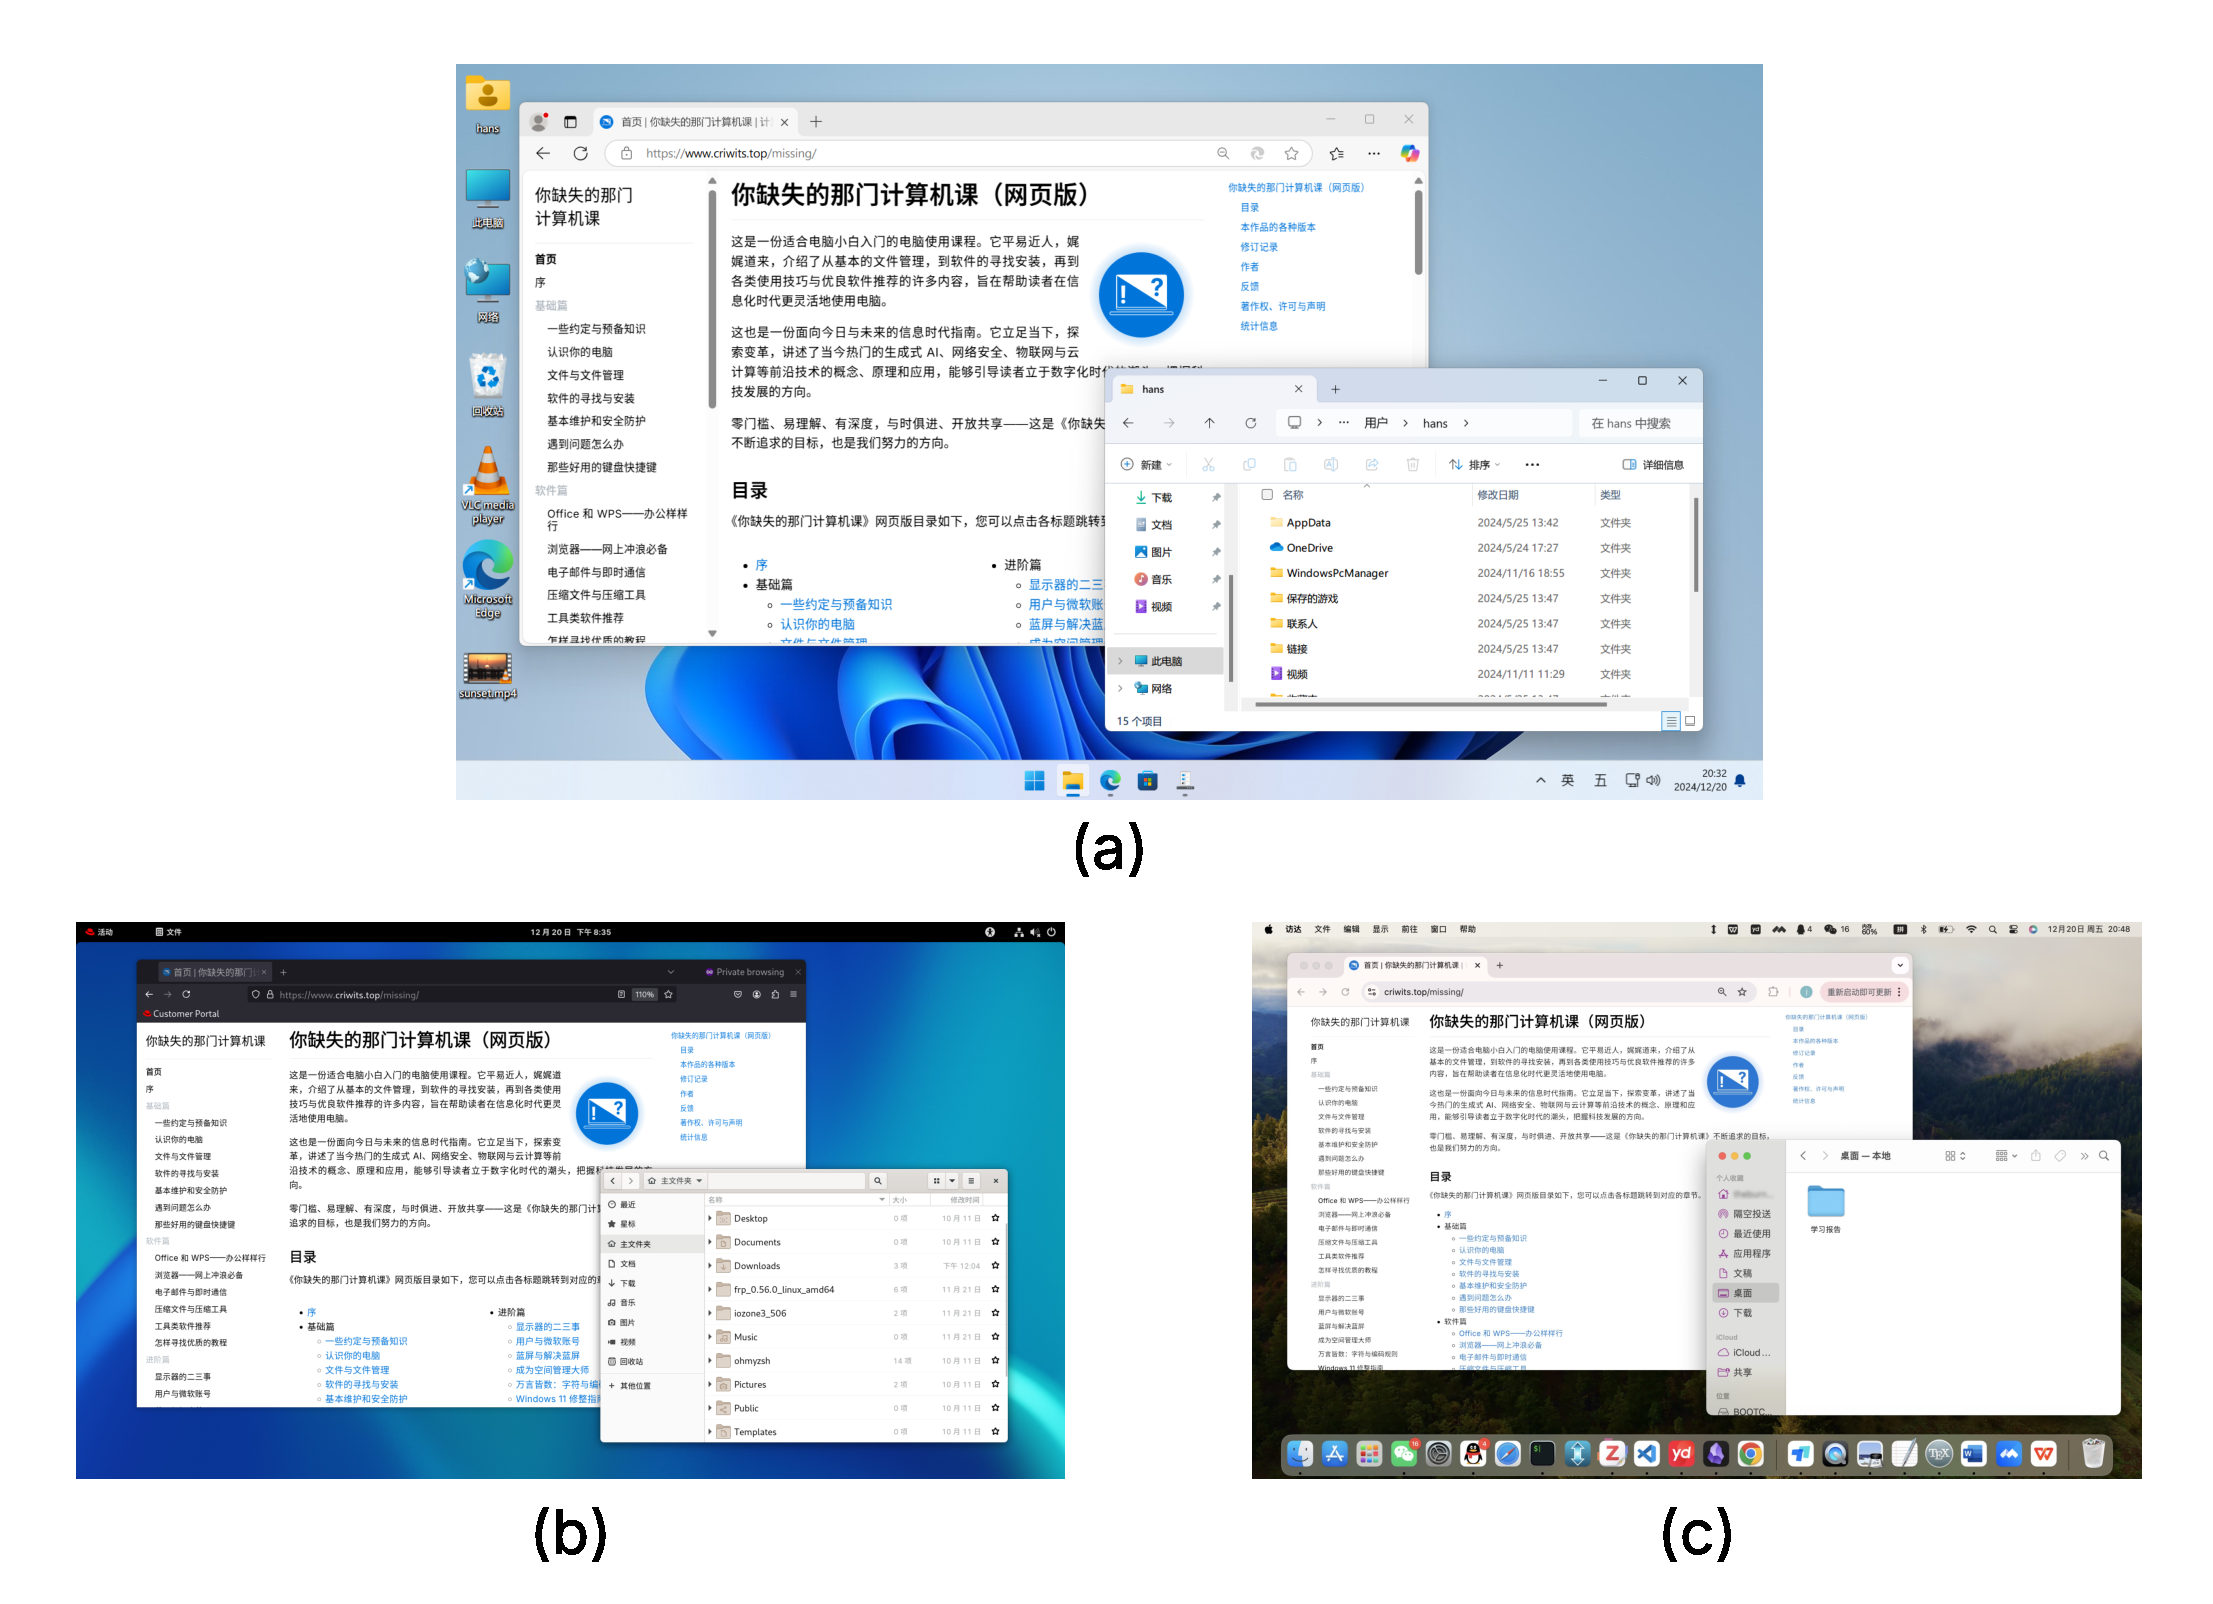
\includegraphics[width=.8\textwidth]{assets/basic/Three_systems.pdf}
  \caption{三大主流电脑操作系统}
  \label{fig:Three_systems}
\end{figure}

\subsection{Windows 操作系统}

我们绝大多数人都在使用 Windows 操作系统,《你缺计课》亦是一套基于 Windows 的电脑教程。所谓「Windows XP」「Windows 7」和「Windows 10」则是 Windows 操作系统的不同版本。

Windows 由美国的微软公司所开发,诞生于 1985 年。到今天(2024 年),Windows 已经经历了数个大版本的更新\footnote{关于 Windows 的一点点更新历史,可以参见“\nameref{cha:recover-from-bsod}”一章。}。今天,除了苹果以外几乎所有品牌的个人电脑都运行着 Windows 系统。目前最新的 Windows 版本是 Windows 11(发布于 2021 年 10 月 5 日),它与 Windows 10(发布于 2015 年 7 月 29 日)一同占领了大部分电脑。在有些地方,一些稍旧的计算机运行着 Windows 7,而更老的 Windows 版本(如 Windows XP)目前已经鲜有使用。不同版本 Windows 系统之间会有操作细节、使用体验上的不同,不过往往最直观的不同是它们的外观。下图中,(a) 和 (b) 分别展示了 Windows 11 和 Windows 10 的界面。

\begin{figure}[htb!]
  \centering
  \includegraphics[width=.9\textwidth]{assets/basic/Win_11_and_10.pdf}
  \caption{如今的两大Windows}
  \label{fig:Win_11_and_10}
\end{figure}

通过右键桌面上的【此电脑】并点选【属性】,或打开系统设置,选择【系统】→【系统信息】(Windows 10 则是【关于】),你可以看到自己电脑 Windows 系统的版本。

\begin{figure}[htb!]
  \centering
  \includegraphics[width=.7\textwidth]{assets/basic/Check_Windows_version.png}
  \caption{检查 Windows 系统版本}
  \label{fig:check-windows-version}
\end{figure}

\regcolor{本书假定读者使用的系统是 Windows 11 或者 Windows 10,其中所有的操作都是基于 Windows 11 或者 Windows 10 简体中文版系统来描述的。}不过,本书所介绍的知识是通用的,如果你使用的是 Windows 7、Windows 8 或者 Windows 8.1,本书提到的多数操作你也能正常使用。一些明确仅能用于 Windows 10 和/或 Windows 11 的操作和技巧一般会特别标注。

\practice

\begin{enumerate}
  \item 通过任务管理器和【此电脑】→【属性】,查看自己电脑的 Windows 版本、CPU 型号和核心数、内存大小、硬盘大小和类型、显卡大小和类型。
  \item 你使用的是游戏本还是轻薄本?亦或是介于二者之间的所谓「全能本」?尝试翻到笔记本的底面,上网搜索它底面所写的型号,了解关于你自己机器的更多信息。
  \item 你对「电路」的认知有多少?你是否好奇 CPU 是怎么运作的?从开关、导线、电池、灯泡组成的最简单「电路」到几乎无所不能「电脑」之间到底发生了什么奇妙的变化?在本书超越篇的\nameref{cha:program-and-arch}一章中,我们会简要向你进一步介绍这些问题。但限于《你缺计课》篇幅,我们是没法完全告诉你这些的。但是,你若有兴趣,可以去学习「电路电子技术」「计算机体系结构」「计算光刻」「纳米测量技术」等相关内容。近年来,国际形势风云变幻,我国在芯片领域仍然存在许多短板。我们希望越来越多的有志青年能投身于包括但不限于体系结构、硬件组成、数字电路乃至微电子、集成电路制造、半导体材料等领域,为我国芯片行业「补上短板」贡献自己的力量。
\end{enumerate}

\chapter{文件与文件管理}
\label{cha:file-and-file-management}

\begin{intro}
  一直以来,「文件管理」都是困扰着许多电脑用户,尤其是初学者的一大难题。看完本章,你将可以找到下面这些问题的答案:
  \begin{itemize}
    \item C 盘、D 盘都是什么?为什么有人建议把软件装到 D 盘里?电脑空间总是不够用,怎么办?
    \item 「扩展名」是什么?「打开方式」又是什么?为什么有时候我电脑上的 Word 文档突然打不开了?
    \item 我应该如何管理好自己的文件?
  \end{itemize}
\end{intro}

如\chapref{cha:computer-and-its-components}一章所言,硬盘是电脑中存放数据的地方,而「文件」则是数据存放的具体形式。你所撰写的 Word 文档、制作的 PowerPoint 幻灯片、从网上下载的图片和视频,乃至各个软件本身,都以文件的形式存储在硬盘上。

本章,我们将具体介绍「文件」以及文件的管理。这是《你缺计课》中需要动手实践的第一章,更是我们合理、有效地使用电脑的第一课。

\section{硬盘的分区}

双击桌面上的【此电脑】,就能打开「\regcolor{文件资源管理器}」,简称「\regcolor{资源管理器}」。在其中,我们可以看到一个或几个「盘」,例如 C 盘、D 盘等。这样的「盘」学名叫做「分区」,顾名思义,它们是将硬盘上的空间人为地划分成了一些子空间。

\begin{note}
  如果你的电脑上没有【此电脑】图标,请先按\chapref{cha:computer-and-its-components}中的方法让它显示在桌面上。
\end{note}

\begin{figure}[htb!]
  \centering
  \includegraphics[width=.8\textwidth]{assets/basic/Partitions.png}
  \caption{电脑上的两个分区}
  \label{fig:Partitions1-2}
\end{figure}

例如,上图是一台电脑「文件资源管理器」中显示的分区。可以看到,这两个分区一个大小为 429 GB,另一个大小为 470 GB,相加为 899 GB——这是这台电脑的硬盘可用总空间。

划分分区的意义,在于帮助我们更好地管理文件。分区划分之后,各个分区之间就仿佛被隔离开来了。即使我们「格式化」一个分区(这样会删除这个分区中的所有文件),也不会影响另外一个分区里面的文件。

\begin{figure}[htb!]
  \centering
  \includegraphics[width=.9\textwidth]{assets/basic/Partition_structure.pdf}
  \caption{分区的结构}
  \label{fig:Partition_structure}
\end{figure}

在 Windows 系统中,分区会被给予两个标识符,或者说「名字」:

\begin{itemize}
  \item 一个是「\regcolor{盘符}」,盘符是一个英文字母加上冒号 \MissingVerb{:} 构成的。我们所称呼的「C 盘」「D 盘」正是指盘符中的那个字母。如上图,左方分区的盘符是 \MissingVerb{C:} ,右方分区的盘符是 \MissingVerb{D:} 。盘符一般在被指定之后就不方便更换了。如今的 Windows 系统中,我们使用的盘符都是从字母 C 开始\footnote{这是因为 A 和 B 两个盘符在过去是留给「软盘」的,但软盘早就已经成为历史了,不过这个习惯却保留了下来。}的。
  \item 另一个是「\regcolor{卷标}」,这是一个可选的标识符,它是一定长度的文本。上图中的 C 盘,卷标就是「本地磁盘」。盘符的作用是让系统和软件识别分区,而卷标的作用是帮助我们用户更加直观地了解分区的作用,因而卷标是可以随时更换的。事实上,通过右键某一分区,选择【重命名】,就可以更换卷标了。如果你什么都不写,它默认显示成「本地磁盘」。
\end{itemize}

\begin{figure}[htb!]
  \centering
  \includegraphics[width=.5\textwidth]{assets/basic/Partition_labels.png}
  \caption{盘符与卷标}
  \label{fig:Partition_labels}
\end{figure}

我们在\chapref{cha:computer-and-its-components}中提到,操作系统本身也是一个大软件,那么这个软件放在硬盘上的哪呢?对于 Windows 而言,\regcolor{整个 Windows 系统默认放在 C 盘里}。双击打开电脑 C 盘,你会看到一些你可能不熟悉的文件夹,例如 \MissingVerb{Windows} 文件夹,Windows 系统自己的许多文件就存在其中。

也许你曾经听过「不要把软件安装到 C 盘」「不要把自己的数据放在 C 盘」这样的说法。这种说法是有一定道理的:如果你的 C 盘总空间较小(这在以前是很常见的情况),而 Windows 系统本身就很庞大,且系统自身工作产生的一些文件也会被自动地放在 C 盘内,这导致 C 盘本身空间很容易变得局促。这时,如果我们还将大量的软件装在 C 盘,就会让 C 盘更加不堪重负,结果就是——满了。

在本章的后续部分,以及\chapref{cha:software-installation}中,我们会详细介绍我们如何比较妥善地利用各个分区。如果你的 C 盘空间已经不足,那么请参考\chapref{cha:manage-storage}中的方法,来释放 C 盘的空间。

\begin{note}
  如果你打开「此电脑」之后,发现自己电脑上只有一个 C 盘,这说明你的电脑磁盘只有一个分区。一些品牌的新电脑出厂时就是这样的设置。如果你想要在 C 盘之后分出一个新的分区,可以参考\chapref{cha:new-laptop-setup}中的方法。如果前面的方法不行,或者你想进行更高级的分区调整(例如调整大小),则需要参见进阶篇的\chapref{cha:manage-storage}。
\end{note}

\section{文件、文件名和文件类型}

\begin{wrapfigure}[5]{r}{7.2cm}
  \centering
  \includegraphics[width=7cm]{assets/basic/5_files.png}
  \caption{一些文件}
  \label{fig:5_files}
\end{wrapfigure}

「文件」是数据存储在硬盘上的形式。这么说可能有些抽象,直观地说,文件就是我们在资源管理器里看到的,像\autoref{fig:5_files} 里面的这些东西。

文件有自己的名字,称为「文件名」。在 Windows 系统中,文件名可以分成三个部分:

\begin{itemize}
  \item 「主名」是指文件名中,「点号」之前的部分。这部分内容可以自定,相当于人类的姓名。上图中,\MissingVerb{数字逻辑设计第 13 讲} 和 \MissingVerb{Obsidian.1.5.11} 等都是文件的主名。
  \item 「点号」是指文件名中间\regcolor{最后一个} \MissingVerb{.}。
  \item 「扩展名」是指文件名中,点号之后的部分\cprotect\footnote{有时候我们称呼文件的扩展名时也会把点号包含进去。下面两种说法是等价的:
    \begin{itemize}
      \item 某文件的扩展名是 \MissingVerb{txt}。
      \item 某文件的扩展名是 \MissingVerb{.txt}。
    \end{itemize}
  }。扩展名指示文件的类型,它会告诉操作系统,这个文件应该用什么方式来打开。例如,上图中 \MissingVerb{本科毕业论文(设计)写作指南(理工类).doc} 中的 \MissingVerb{doc} 就是这个文件的扩展名,它说明这个文件是一个 Word 文档,应该使用 Word 或 WPS 等软件打开。
\end{itemize}

\begin{note}
  如果你的电脑上,文件的扩展名没有显示出来(也就是说你只能看到文件的主名),像这样:

  \begin{center}
    \includegraphics[width=7cm]{assets/basic/5_files_not_showing_extensions.png}
    \captionof{figure}{隐藏扩展名的文件}
    \label{fig:5_files_not_showing_extensions}
  \end{center}

  在 Windows 10 中请点选文件夹窗口上方的【查看】选项卡,然后勾选【文件扩展名】这一项:

  \begin{center}
    \includegraphics[width=.6\textwidth]{assets/basic/Windows_10_set_full_filename.png}
    \captionof{figure}{在Windows 10中显示文件扩展名}
    \label{fig:Windows_10_set_full_filename}
  \end{center}

  在 Windows 11 中请点选文件夹窗口上方的【查看】菜单,然后勾选【显示】→【文件扩展名】:

  \begin{center}
    \includegraphics[width=.6\textwidth]{assets/basic/Windows_11_set_full_filename.png}
    \captionof{figure}{在Windows 11中显示文件扩展名}
    \label{fig:Windows_11_set_full_filename}
  \end{center}
\end{note}

扩展名也可以人为改变,但这样往往会出问题——试想,\autoref{fig:5_files} 中的 \MissingVerb{数字逻辑设计第 13 讲.ppt},本来是一个 \MissingVerb{ppt} 文件,即 PowerPoint 幻灯片,应该用 PowerPoint 或 WPS 打开。如果你强行把它改成 \MissingVerb{txt},系统就会用记事本来打开一个幻灯片——用错误的工具打开文件。因此,扩展名不能随便改,因为改了之后系统就会用错误的工具去打开它。右键某一文件,选择【重命名】,你会看到系统会自动帮你选中文件的主名,而不选中扩展名。如果你执意更改文件的扩展名,系统会发出一个提示:

\begin{figure}[htb!]
  \centering
  \includegraphics[width=6cm]{assets/basic/Warning_when_changing_extension.png}
  \caption{尝试更改扩展名……}
  \label{fig:Warning_when_changing_extension}
\end{figure}

「那既然这样,我不想不小心突然间改掉文件的扩展名,还不如让扩展名不显示呢。」如果你有这样的想法,那么另一重危险正悄然降临。且看下面的两个文件:

\begin{figure}[htb!]
  \centering
  \begin{minipage}{.48\textwidth}
    \centering
    \includegraphics[width=.9\textwidth]{assets/basic/fake_doc.png}
    \caption{两个同名文件?!}
    \label{fig:fake_doc}
  \end{minipage}
  \begin{minipage}{.48\textwidth}
    \centering
    \includegraphics[width=.9\textwidth]{assets/basic/fake_doc_revealed.png}
    \caption{揭示扩展名后}
    \label{fig:fake_doc_revealed}
  \end{minipage}
\end{figure}

这两个「高数速成秘籍」看起来完全一样,就是两个正常的 Word 文档,但众所周知,一个目录下不可能存在两个文件名相同的文件,显然这里面必然有猫腻。现在打开文件扩展名,这两个文件的名称变成了下面这个样子,可见,其中一个居然是可执行文件(\MissingVerb{exe})格式,即一个应用程序(详见下文),只是图标故意被做成了 Word 文档的样子。所以,看不到扩展名的话,指不定哪天有居心叵测的人发来一个这样伪装的病毒,那可就不好了。

\section{文件夹、路径和目录}

「文件夹」是一个用来存放其他文件的结构。不妨想象一下现实中的文件夹:在一个文件夹中,可以放很多各类文件。而电脑中的文件夹除了能放文件之外,还可以放很多的「子文件夹」,即文件夹里面的文件夹。这个过程可以循环重复,因而一个文件夹的内部结构可以相当错综复杂。

假设在 D 盘里的 \MissingVerb{missing} 文件夹之中,有一个叫做 \MissingVerb{源文件} 的子文件夹,在这个子文件夹中有一个文件叫 \MissingVerb{第三章.docx},我们用这种方式表示这个 \MissingVerb{第三章.docx} 文件在整个电脑中的位置:

\begin{MissingVerbatim}
  D:\missing\源文件\第三章.docx
\end{MissingVerbatim}

这一长串东西可以唯一确定地表示出 \MissingVerb{第三章.docx} 这个文件在电脑中的具体位置,我们把一长串东西称为 \MissingVerb{第三章.docx} 这个文件的「路径」(严格来说叫做「绝对路径」)。不难发现,路径是从分区(也就是「盘」)开始,用反斜杠 \MissingVerb{\} 作为分隔,一级一级文件夹地展开,最后到具体的文件。类似的,不只是文件,文件夹的路径也可以用这样的方式来表示,例如
\begin{MissingVerbatim}
  D:\missing\源文件
\end{MissingVerbatim}
\noindent{}表示的就是 \MissingVerb{源文件} 这个文件夹在电脑中的位置。一个文件或文件夹的路径是唯一确定的;一个路径也能唯一确定一个文件或文件夹。

也许你有听说过「目录」这个名字。其实「目录」就是文件夹。例如说「打开目录 \MissingVerb{D:\missing\public}」指的就是打开 D 盘中 \MissingVerb{missing} 文件夹里的 \MissingVerb{public} 文件夹。

目录(文件夹)一层一层的结构可以像\autoref{fig:Tree} 这样从上到下画出来,称作「目录树」。树的特点是从一个「根」开始,生长出许多的枝叶,这和文件夹「一层套一层」的结构是一致的。下图便展示了一棵目录树,它的根是文件夹 \MissingVerb{Documents},而其他的文件和文件夹则是它的枝叶。与现实中的树不同的是,目录树是倒着的,根在上,叶子在下。

\begin{figure}[htb!]
  \centering
  \includegraphics[width=.5\textwidth]{assets/basic/Tree.png}
  \caption{目录树}
  \label{fig:Tree}
\end{figure}

在目录树这种形式中,文件夹之间是「上下级」的关系,故「文件 A 在文件夹 B 中」也可以称作「文件 A 在文件夹 B 下」或者「A 在目录 B 下」甚至是「A 在 B 下」。也就是说,「下」这个字就是「在……里」的意思。

借助目录树这样的结构,我们就能理解「根目录」这个概念了。一个盘的「根目录」就指的是这个盘本身那一级目录——恰好是目录树的根,例如 C 盘根目录就指的是路径 \MissingVerb{C:\} 。

\section{程序本身——可执行文件(\MissingTT{exe} 文件)}

\begin{wrapfigure}{r}{5.2cm}
  \centering
  \includegraphics[width=5cm]{assets/basic/NCM_directory.png}
  \caption{网易云音乐的目录}
  \label{fig:NCM_directory}
\end{wrapfigure}

这一节我们介绍一种类型特殊的文件——「可执行文件」。我们提到,数据是以文件的形式存储在硬盘上的,比如你所撰写的 Word 文档,它们都存储成了扩展名为 \MissingVerb{doc} 或者 \MissingVerb{docx} 的文件;你所下载的图片,它们的扩展名则往往是 \MissingVerb{jpg} 、 \MissingVerb{png} 或者 \MissingVerb{gif} 。而我们又提到,软件也是以文件的形式存储在硬盘上的。那么,软件本身是什么格式的文件呢?

一个软件的核心是一个或多个「程序」,而程序是以「可执行文件」的形式存储的。\regcolor{普通的文件,需要用其他的某个软件才能正常打开;而「可执行文件」双击就能运行自身,这就是「可执行」(Executable)的意思。}

可执行文件的扩展名是 \MissingVerb{exe} 。对于这种类型的文件,系统不会想着用别的软件去打开它,而是直接运行它自身。可执行文件有时被直接称为「程序文件」或者「程序」。

需要注意的是,电脑上的一款软件可能不是仅仅只有一个 \MissingVerb{exe} 文件。例如,右图是软件「网易云音乐」所在的文件夹中的一部分。

可以看到,网易云音乐有着这些文件:

\begin{itemize}
  \item 可执行文件 \MissingVerb{cloudmusic.exe} ,这个是「网易云音乐」的主程序。
  \item 可执行文件 \MissingVerb{cloudmusic_reporter.exe},\MissingVerb{cloudmusic_util.exe} 等。这些文件是软件运行时的其他辅助程序。它们往往无法单独运行,而 \MissingVerb{cloudmusic.exe} 这个主程序脱离它们也不能正常运行。
  \item 一大堆的 \MissingVerb{dll} 和其他格式的文件。这些是软件工作时不可或缺的依赖文件。
  \item 一些子文件夹,存储着软件运行需要的一些资源。
\end{itemize}

每次我们启动网易云音乐,运行的都是 \MissingVerb{cloudmusic.exe} 这个可执行文件。然而,这个文件的运行离不开放在它边上的那一堆辅助文件——如果你把 \MissingVerb{cloudmusic.exe} 复制到另外的一个地方,双击运行,大概率会直接报错;即使不报错,功能也必不完全正常。在后续的章节,我们在介绍软件的安装与卸载时,会继续提到这件事。

\begin{note}
  好奇这 \MissingVerb{exe} 文件里面到底是什么?答案将在超越篇的\chapref{cha:program-and-arch}揭晓。
\end{note}

\section{文件的「替身」——快捷方式}

你是怎么启动网易云音乐的呢?

一般来说,我们会双击桌面上的「网易云音乐」,或者点击开始菜单中的「网易云音乐」。然而,这些地方看到的「网易云音乐」,都不是这个软件的本体,而是另一种称为「快捷方式」的特殊文件。「快捷方式」可以看成某个具体文件的单向「指针」或者说「替身」,打开快捷方式就相当于打开了本体。

\begin{figure}[htb!]
  \centering
  \includegraphics[width=10cm]{assets/basic/Link.pdf}
  \caption{快捷方式}
  \label{fig:Link}
\end{figure}

快捷方式的扩展名是 \MissingVerb{lnk},但实际上不可见\cprotect\footnote{千万不要手动把一个正常文件的扩展名改成 \MissingVerb{lnk},否则就很难改回来了。}。我们桌面上的「网易云音乐」,指向的正是网易云音乐软件目录下的那个 \MissingVerb{cloudmusic.exe} 文件。右击桌面上的【网易云音乐】,选择【属性】,会弹出这个快捷方式的详细信息,如\autoref{fig:Link_properties} 所示。

\begin{wrapfigure}[12]{r}{6cm}
  \centering
  \includegraphics[width=5.8cm]{assets/basic/Link_properties.png}
  \caption{「网易云音乐」的快捷方式}
  \label{fig:Link_properties}
\end{wrapfigure}

其中「目标」一栏填写的正是 \MissingVerb{cloudmusic.exe} 这个可执行文件,即「网易云音乐」的主程序的路径:

\begin{MissingVerbatim}
  D:\Program Files (x86)\Netease\CloudMusic\cloudmusic.exe
\end{MissingVerbatim}

因此,双击打开这个「网易云音乐」快捷方式,就等同于打开 \MissingVerb{cloudmusic.exe} 这个文件。\cprotect\regcolor{如果你删掉了这个快捷方式,它并不会影响 \MissingVerb{cloudmusic.exe} 这个文件,不会影响你电脑上安装的网易云音乐本身。}因此,卸载软件并非仅仅把桌面上的「快捷方式」删掉就完事了,而是需要通过借助卸载工具。我们将在\chapref{cha:basic-maintenance}中介绍。

所有类型的文件以及文件夹都可以制作无数个快捷方式。如果你想给自己的某个文件/文件夹制作一个快捷方式,只需右键它,选择【发送到】→【桌面快捷方式】,就能在桌面生成一个指向这个文件的快捷方式了。这个快捷方式可以挪到系统的任何地方,也可以复制粘贴出很多个副本。它们全都指向原来的那个文件本身。

一般来说,快捷方式的图标左下角会有一个「↗」符号。这个符号标志着这个文件并非某文件本身而是一个快捷方式。

\section{合多为一,精简空间——压缩文件}

「压缩文件」又称「压缩包」,是一种常用的文件类型。人们可以\regcolor{利用「压缩工具」这种软件,将一批松散的文件和文件夹「打包」成一个压缩文件}\footnote{也可以打包成多个文件,称为「分卷压缩」,详见\chapref{cha:archive-formats-and-tools}一章。}。假设你有 8 个文件夹以及 7 个文件一共 15 个项目,你想一次性把它们分享给别人,那么把它们打包成一个压缩文件不失是一种好的选择。

\begin{figure}[htb!]
  \centering
  \includegraphics[width=.7\textwidth]{assets/basic/Compress_and_decompress.pdf}
  \caption{压缩与解压}
  \label{fig:Compress_and_decompress}
\end{figure}

压缩文件有很多种类,常见的有 \MissingVerb{zip} 文件和 \MissingVerb{rar} 文件,但后者的压缩软件是收费的\cprotect\footnote{具体来说,大多数压缩工具都可以解压 \MissingVerb{rar} 格式的压缩包,但只有 WinRAR 这一款压缩工具可以制作这种格式的压缩包;而这款工具是收费的。详见\chapref{cha:archive-formats-and-tools}。}。我们建议在与他人交换文件的时候,使用\MissingVerb{zip} 格式打包。

当收到一个压缩文件时,我们一般需要将它解压,来还原出原始的文件。如果你电脑上已经安装有压缩工具,那么可以右击压缩文件,选择类似「解压到当前文件夹」\footnote{部分压缩工具称「解压」为「提取」,而有的压缩工具称「解压到此处」,它们的意思是一样的。}或者「解压到 \MissingVerb{<文件名>\}」的选项。这两类选项的不同是:

\begin{itemize}
  \item 「解压到当前文件夹」会把压缩文件里的内容直接放在压缩文件的同一目录下。例如,如果一个压缩文件 \MissingVerb{archive.zip} 里面有 \MissingVerb{a.txt} 和 \MissingVerb{b.txt} 两个文件,选择此选项,解压后 \MissingVerb{a.txt} 和 \MissingVerb{b.txt} 都和 \MissingVerb{archive.zip} 在同一级目录。
  \item 「解压到 \MissingVerb{<文件名>\}」会把压缩文件里的内容放在一个子文件夹里面。在上面的例子中选择这个选项,会在 \MissingVerb{archive.zip} 的同一级目录新建一个文件夹 \MissingVerb{archive},然后把 \MissingVerb{a.txt} 和 \MissingVerb{b.txt} 放在 \MissingVerb{archive} 文件夹下。
\end{itemize}

\begin{figure}[htb!]
  \centering
  \includegraphics[width=.6\textwidth]{assets/basic/Extract.pdf}
  \caption{不同的解压指令}
  \label{fig:Extract}
\end{figure}

我们建议,为了不让自己的工作目录变得混乱,\cprotect\regcolor{尽量使用「解压到 \MissingVerb{<文件名>\}」}。

\begin{note}
  想想为什么?
\end{note}

如果我们只是想查看一个压缩文件的内容,而不把它解压,可以直接双击打开它,压缩软件会展示出其中的内容。双击这里面的单个文件可以临时取出这一个文件并打开它,拖拽其中的单个文件到其他地方可以只取出这一个文件而不解压整个压缩文件。但是,\regcolor{若你想运行压缩文件中的程序(可执行文件),请一定要完整解压文件},否则程序很可能无法正常工作。

\begin{figure}[htb!]
  \centering
  \includegraphics[width=.7\textwidth]{assets/basic/Opened_archive.png}
  \caption{打开一个压缩包}
  \label{}
\end{figure}

当你想制作一个压缩文件时,可以先选中你要打包的所有文件和文件夹,右击它们并选择类似「新建压缩包」或「压缩为 \MissingVerb{<文件名>}」的选项。压缩工具可能会提示你设置一些参数,例如压缩格式(推荐 \MissingVerb{zip} 格式)、压缩后的文件的文件名以及压缩方式。

有关压缩文件和压缩工具的更多细节,请参见本书软件篇的\chapref{cha:archive-formats-and-tools}一章。

\section{文件的打开方式}

在前文中说到,不同类型的文件需要用不同的软件来打开。对于一个特定的文件类型,打开它的软件称为它的「打开方式」。如果打开方式不对,就会出现问题。

容易想到,Word 文档 \MissingVerb{doc} 和 \MissingVerb{docx} 文件的打开方式就是 Word 软件或者 WPS 软件;图片 \MissingVerb{jpg}、 \MissingVerb{png} 等的打开方式就是各种看图软件;PDF 文档 \MissingVerb{pdf} 的打开方式就是 PDF 阅读器,例如 Acrobat 或者 SumatraPDF……

\begin{note}
  可执行文件的打开方式是什么呢?因为它们自己就是程序本身,所以没有「打开方式」的概念。
\end{note}

\begin{table}[htb!]
  \centering
  \caption{神奇的「表」}
  \label{tab:regtable}
  \begin{tblr}{
    colspec = X[.8]X[1.2]X[6.2],
    cells = {c, m},
    cell{2-Y}{Z} = {j},
    row{1} = {fg = white, bg = missing, font = \bfseries},
    row{even} = {MissingSkyBlue},
  }
    \toprule
    扩展名 & 用什么软件打开 & 软件主程序的路径在哪 \\
    \midrule
    \MissingTT{txt} & 记事本 & \MissingTT{C:\textbackslash{}Windows\textbackslash{}system32\textbackslash{}notepad.exe}  \\
    \MissingTT{docx} & Word & \MissingTT{C:\textbackslash{}Program Files\textbackslash{}Microsoft Office\textbackslash{}root\textbackslash{}Office16\textbackslash{}WINWORD.EXE}  \\
    \MissingTT{mp3} & 网易云音乐 & \MissingTT{D:\textbackslash{}Program Files (x86)\textbackslash{}Netease\textbackslash{}CloudMusic\textbackslash{}cloudmusic.exe}  \\
    …… & …… & …… \\
    \bottomrule
  \end{tblr}
\end{table}

系统内部维护有一张「表」,这张表记录了已知的文件类型(扩展名)和对应的打开方式。你可以把这张表想象成\autoref{tab:regtable} 那样。

有了这张表,系统就能自动地帮我们选择文件对应的打开方式。有时,我们不想要用这张表帮我们预置的方式来打开文件。比如,打开 \MissingVerb{png} 图片的默认方式是「照片」软件,但如果我们想\textbf{暂时}用「画图」来打开它,我们可以这样做:

\begin{itemize}
  \item 右键要打开的这个 \MissingVerb{jpg} 文件,选择【打开方式】,在里面选择【画图】,如\autoref{fig:Open_with} 所示。
  \item 如果上一步找不到「画图」,那么选择【打开方式】→【选择其他应用】。然后在弹出的对话框中寻找并点击【画图】。然后,对于 Windows 10,不要勾选【始终使用此应用打开 \MissingVerb{.png} 文件】,直接点击【确定】;对于 Windows 11,点击【仅一次】,如\autoref{fig:Open_with_dialog} 所示。
    \begin{figure}[htb!]
      \centering
      \begin{minipage}{.55\textwidth}
        \centering
        \includegraphics[width=.98\textwidth]{assets/basic/Open_with.png}
        \caption{更改打开方式}
        \label{fig:Open_with}
      \end{minipage}
      \begin{minipage}{.43\textwidth}
        \includegraphics[width=.98\textwidth]{assets/basic/Open_with_dialog.png}
        \caption{选择更多应用}
        \label{fig:Open_with_dialog}
      \end{minipage}
    \end{figure}
  \item 如果你想用自己安装的软件打开这个文件,而上一步的界面找不到那个软件,例如 Adobe Photoshop,那么可能需要手动找到 Adobe Photoshop 的可执行文件,也就是它的 \MissingVerb{exe} 文件。这个文件的路径——也就是软件的安装路径——在下一章我们会提到,一般来说是在 \MissingVerb{C:\Program Files} 或者 \MissingVerb{C:\Program Files (x86)} 之下的某个文件夹中。
\end{itemize}

\regcolor{如果你想永久地指派某一文件的打开方式,则可以在上面步骤的基础上,Windows 11 点击【始终】,Windows 10 则勾选【始终使用此应用打开 \MissingTT{XXX} 文件】。}这样,系统内部的那张表就会被更改,系统以后都会用你指派的新应用来打开这种文件。

除了你手动更改之外,这张表还可能在这些情况被更改:

\begin{itemize}
  \item 系统安装更新,即 Windows 更新之后,这张表可能会被重置而丢失一些项目,造成某些文件突然无法打开。这有可能是由于你使用的对应软件并不是原版,而是某种「精简版」。
  \item 新安装一个软件时,软件安装程序可能写入新的表项,来为即将安装的新软件的文件类型配置打开方式。
  \item Windows 本身的行为。例如,Windows 可能会时不时用 Microsoft Edge 代替其他软件来打开网页文件和 \MissingVerb{pdf} 文件等。\CJKsout*{(微软你坏事做尽)}
\end{itemize}

如果你的文件关联某天突然失效,即某种类型的文件突然无法打开,但对应的软件工作正常,那么可以考虑是否是上面的原因。

\section{管理好你的文件}

管理好我们的文件,不外乎两个方面:

\begin{itemize}
  \item \regcolor{将自己的文件整理归类。}比起将所有文件随手乱放在桌面上,如果我们将自己的文件按它们的性质、类别等归类存放,必然有助于提升我们的工作效率。
  \item \regcolor{妥善利用各个分区,如果可行,尽量不把大量重要文件放在 C 盘。}在前文我们说了,C 盘是 Windows 系统整个所在的地方。如果 C 盘空间本身就有限,在 C 盘存放大量数据会显著增加空间压力。另一方面,尽管发生这种情况的概率很低,但当我们的电脑因为这样或那样的原因损坏,而需要重新安装系统的时候,你会不得不失去 C 盘的所有文件——因为多数时候,我们安装系统的第一步就是格式化 C 盘。
\end{itemize}

\subsection{分区的选择}

取决于你电脑硬盘的大小以及分区的情况,我们推荐了一些方案:

\begin{itemize}
  \item 如果你的电脑只有一个 C 盘:
  \begin{itemize}
    \item 若你的总容量小于 300 GB,建议不要再分额外的分区,将你的文件直接存放在 C 盘。同时,你可以使用移动硬盘或各种「网盘」来备份好你的重要数据。
    \item 如果你的总容量在 300 GB—500 GB,可以选择为 C 盘留下 200 GB 左右,并将剩余的空间分出一个新的分区(D 盘)。然后,在 D 盘存放你的文件。
      \begin{note}
        如果你想要在 C 盘之后分出一个新的分区,可以参考\chapref{cha:new-laptop-setup}中的方法。如果前面的方法不行,或者你想进行更高级的分区调整(例如调整大小),则需要参见进阶篇的\chapref{cha:manage-storage}。
      \end{note}
    \item 如果你的总容量在 500 GB 以上,建议为 C 盘留出 400 GB—500 GB 的空间,再将剩余的空间按自己的喜好,分出一个或多个新的分区(D 盘、E 盘……)。然后,在这些分区存放你的文件。
  \end{itemize}
  \item 如果你的电脑已经有多个分区(C 盘、D 盘……),可以先在「任务管理器」中,查看每个分区对应的硬盘:
  \begin{itemize}
    \item 如果你只有一块硬盘,通常这种情况下,你的 C 盘不会很大,建议直接在 D 盘和之后的分区存放你的文件。
    \item 如果你有多块硬盘,并且所有硬盘都是 SSD,我们亦建议你使用 D 盘和之后的分区存放文件。
    \item 如果你有多块硬盘,并且有的分区在 SSD 上,有的分区在 HDD 上,我们建议你将常用的软件和数据放在位于 SSD 的分区上(包括 C 盘),而将其他大型软件和不那么常用的数据放在位于 HDD 的分区上。
  \end{itemize}
\end{itemize}

当然,这些方案并非绝对,你可以根据自己的情况选择,适度调整分配大小。

\subsection{为文件安家}

为了给文件安家,我们首先需要挑选一个合适的位置。\regcolor{如果你打算把文件放在 C 盘,可以使用 Windows 为你提供的一系列「已知文件夹」(Known Folder)},即「文档」「视频」「下载」等。Windows 11 系统中,你可以在【此电脑】窗口的左侧看到这些文件夹,如\autoref{fig:Win11_user_folders};而在 Windows 10 中,双击桌面上的【此电脑】,展开【文件夹】折叠项看到这些文件夹,如\autoref{fig:User_directories}。

\begin{figure}[htb!]
  \centering
  \begin{minipage}{.49\textwidth}
    \centering
    \includegraphics[width=.98\textwidth]{assets/basic/Win11_user_folders.png}
    \caption{Windows 11 的已知文件夹}
    \label{fig:Win11_user_folders}
  \end{minipage}
  \begin{minipage}{.49\textwidth}
    \centering
    \includegraphics[width=.98\textwidth]{assets/basic/User_directories.png}
    \caption{Windows 10 的已知文件夹}
    \label{fig:User_directories}
  \end{minipage}
\end{figure}

默认情况下,\cprotect\regcolor{已知文件夹的实际位置在 \MissingVerb{C:\用户\<你的用户名>},这是你的「用户配置文件夹」(User Profile Folder,俗称「用户文件夹」)。}除了直接在【此电脑】中查看外,你也可以手动打开这个路径来找到它们。已知文件夹涵盖了「桌面」「文档」「图片」「音乐」「视频」等多种类别,并且都配有形象的图标。如果你计划将自己的文件存放在 C 盘,这些目录是不错的选择。

\begin{warning}
  注意:C 盘作为 Windows 的系统分区,有严格的写保护机制,最好不要把你的文件直接放在 C 盘根目录下。
\end{warning}

如果你打算把自己的文件放到其他的分区,各个分区的根目录都是不错的选择。你可以仿照 Windows 给你的已知文件夹,自己在其他分区的根目录下按类别新建好「文档」「电影」「音频」等文件夹,用来帮助自己整理文件。更进一步,\regcolor{你还可以直接将 Windows 提供给你的这些已知文件夹迁移到其他分区},这样它们的实际位置就不再是 \MissingVerb{C:\用户\<你的用户名>},而是你指定的地方了。例如,如果你想使用 D 盘根目录即 \MissingVerb{D:\} 来存放这些已知文件夹,可以按下面的步骤操作。

\begin{itemize}
  \item 在资源管理器中,右击某个我们想要迁移的文件夹(比如【文档】),选择【属性】,然后切换到【位置】选项卡,如\autoref{fig:Pos_of_Documents}。
    \begin{figure}[htb!]
      \centering
      \includegraphics[width=.7\textwidth]{assets/basic/Pos_of_Documents.png}
      \caption{查看「文档」的位置}
      \label{fig:Pos_of_Documents}
    \end{figure}
  \item 我们将这里文本框中
    \begin{MissingVerbatim}
      C:\Users\<你的用户名>\
    \end{MissingVerbatim}
  \item 这一部分\cprotect\regcolor{(注意:最后一个\MissingVerb{Desktop}、\MissingVerb{Documents}之类的名字不要动!)}\footnote{如果你不小心把一个已知文件夹的位置设置成了某个磁盘的根目录(比如说\MissingTT{D:\textbackslash}),可能很难再改回来。}改成
    \begin{MissingVerbatim}
      D:\
    \end{MissingVerbatim}
    \regcolor{也就是说,对于「桌面」而言,改完之后的完整路径是}
    \begin{MissingVerbatim}
      D:\Documents
    \end{MissingVerbatim}
  \item 点击【应用】,提示「文件夹 ‘\MissingVerb{D:\Desktop}’ 不存在,是否新建该文件夹」,选择【是】。
  \item 紧接着提示「是否要将所有文件从原位置移动到新位置」,选择【是】。
\end{itemize}

一般来说移动操作很快就会完成。完成后,点击【确定】。这样「文档」文件夹就被成功地迁移到了 D 盘,你可以直接在【此电脑】中双击【文档】打开它,也可以打开 \MissingVerb{D:\文档} 来访问,如\autoref{fig:Moved_user_directories} 所示。\regcolor{如果你打算使用 C 盘以外的分区存放自己的文件,我们强烈建议你迁移各已知文件夹到对应的分区},因为它们能帮你更好地管理文件。

\begin{figure}[htb!]
  \centering
  \includegraphics[width=.7\textwidth]{assets/basic/Moved_user_directories.png}
  \caption{移走的已知文件夹}
  \label{fig:Moved_user_directories}
\end{figure}

在找到合适的位置后,我们便可以建立一套自己的分类方法来对文件进行整理和分类。

\begin{itemize}
  \item 例如你有一些「学习资源」,你便可以合适的地方建立一个名为「学习资源」的文件夹,再在其下——无论是按学科(例如「高数」「线代」「物理」),还是按时间(例如「大一上」「大一下」)——建立更多的子文件夹,来为它们进行更为详尽的分类。
  \item 再例如你有许多「大片」,你也可以按照地区、上映时间甚至是主演什么的为它们分类。不过鉴于大片不仅是名气大,占用空间也大,我们推荐腾出一个分区(甚至是一块硬盘)来存放它们。
\end{itemize}

总之,「\regcolor{为你的文件进行合理分类}」与「\regcolor{将你的硬盘进行合理分配}」便是这里的核心思想。

\subsection{定期打扫}

电脑里面的东西总是随着我们的日常使用而越积越多\CJKsout*{(比如微软的更新,一更一大堆;以及 QQ、微信的文件接收文件夹,相信你不一定知道在哪\footnotemark)}\footnotetext{你可以先把一个文件发给自己,然后删掉原始文件,再下回来,就能找到这些接收文件夹的位置(真是曲线救国啊)。},所以定期检查你不需要的东西然后扔掉它们显得尤为重要。

对于系统分区 C 盘来说,你不去动它,它也会被塞入一些诸如系统临时文件、Windows 更新文件等等这些。诸如「火绒安全软件」「360 电脑管家」之类的工具通常都会提供「系统清理」功能,可以帮助你清理这些文件。除此之外,Windows 自身也提供了一个磁盘清理工具。在\chapref{cha:manage-storage}一章中,你将学习到如何使用它来打扫你的 C 盘。

上述各种磁盘清理工具并不会把我们日常中积累的用户文件(例如你收到的课件、文档等)也清理掉,但在日常使用过程中,我们也会不可避免地产生许许多多的冗余文件,或是曾经需要而现在不再需要的文件。这里不妨就来看看你的「下载」文件夹:

\begin{itemize}
  \item 作为一个已知文件夹,它默认在 C 盘,如果你没有按照前文迁移它的话。各大浏览器、新版 QQ、飞书等应用都会把接收到、下载到的文件存在这里;
  \item 点击资源管理器左侧的【下载】,进入 \MissingTT{下载} 文件夹,将其中的所有文件检查一遍,有用的就如上文所述——无论按时间也好还是按类型也好——归类、无用的则直接删除,这就大功告成了;
  \item 进一步而言,如果你不想让各大软件都往 C 盘的这里塞东西,可以参照前文的方法将它迁走,或者在各个应用中设置默认下载文件的存储路径到你喜欢的地方。
\end{itemize}

\begin{note}
  这也解释了为什么我们在前文中提到,如果你决定使用其他分区存放文件,就最好将这些已知文件夹一并迁移。因为根据微软的规范,许多软件都会默认使用它们来存放数据,将它们迁移走可以更好地缓解 C 盘压力。
\end{note}

同样地,在你已经归好类的文件体系中,也要时不时进行检查,删去冗余与无用文件,这样能够保持你的文件系统简而精。《礼记·大学》载:「苟日新,日日新,又日新。」如是而已。

\practice

\begin{enumerate}
  \item 查看自己电脑的几个分区的「卷标」,并依照自己的文件分类习惯修改成自己所喜欢的名字。例如,叫「资料」或者「Files」就比「新加卷」或者没有卷标(会显示「本地磁盘」)要直观得多。
  \item 尝试把一个图片文件的扩展名改成 \MissingVerb{txt},然后用「记事本」打开它。你看到了什么?\CJKunderline*{记得改回来哦!}
  \item 试着根据我们的建议,选择合适的分区运用策略。如果需要,可以试试迁移一部分已知文件夹。
    \begin{warning}
      注意迁移的时候千万看清楚目标路径是完整的 \MissingVerb{D:\Documents}、\MissingVerb{D:\Desktop} 这样的路径,而不是光秃秃的一个 \MissingVerb{D:\}。
    \end{warning}
  \item 整理你的「下载」文件夹。
  \item 选择你自己的几个文件和文件夹,把它们打包成一个压缩文件 \MissingVerb{MyArchive.zip},复制到其他的某个地方,尝试两种不同的解压方式「解压到当前位置」「解压到 \MissingVerb{MyArchive\}」。
  \item 创建一个文档(可以是纯文本文件 \MissingVerb{txt} 或者 Word 文档 \MissingVerb{docx} 等)并写入一些内容,然后制作它的两个快捷方式,并把这两个快捷方式放在两个与源文件都不一样的地方。试着双击打开那两个快捷方式,你发现了什么?删掉两个快捷方式中的一个,源文件被删除了吗?另一个快捷方式还在吗?
\end{enumerate}
\chapter{软件的寻找与安装}
\label{cha:software-installation}

\begin{intro}
  都说电脑离不开软件,可是软件的寻找和安装并非易事——从哪里下?怎么下?下完怎么装?装完怎么办?什么,软件要收费?破解是什么?……这一章将对国内互联网环境下 Windows 软件的下载、安装和配置做一个简单的介绍。看完本章,你或许可以找到下面这些问题的答案,并慢慢对「怎么寻找软件」有一个初步的了解。
  \begin{itemize}
    \item 我想下载某款软件,我应该去哪里找这软件?
    \item 网上全是病毒和垃圾软件,我应该怎么样最大程度保证自己电脑的安全?
    \item 为什么软件下到手还要安装?有的还要破解?为什么这么麻烦?
    \item 电脑里不是有个「Microsoft Store」吗?为什么那里面大多数软件都找不到?
  \end{itemize}
\end{intro}

直到今天,Windows 系统下依然没有一个广泛使用的集中化「应用商店」。与我们使用手机不同,在电脑上,我们若想安装某个软件,多数情况下需要到互联网上寻找软件的「安装包」,再自行将软件安装到电脑上来使用。

这一章,我们将具体介绍如何从网上的万千垃圾软件中下载我们需要的软件,以及软件安装和配置的一些技巧和注意事项。\vspace*{-.5cm}

\section{安装与安装包}

\begin{wrapfigure}[15]{r}{5.2cm}
  \centering
  \raisebox{0pt}[\dimexpr\height-0.6\baselineskip\relax]{\includegraphics[width=5cm]{assets/basic/NCM_directory.png}}
  \caption{「网易云音乐」的目录}
  \label{fig:NCM_directory2}
\end{wrapfigure}

在 Windows 系统上,软件是通过「安装包」来安装到系统上的。如果把软件比作一棵树,那安装包就是这棵树的种子,我们需要借助安装包将软件「种」到电脑上,这个过程就是「安装」。为什么需要安装包,而不直接分发应用本身呢?解答这个问题,就有必要稍微了解一下软件在我们的电脑上的安装过程。

在上一章\chapref{cha:file-and-file-management}中我们看到,一款软件除了主程序(一个 \MissingVerb{exe} 文件)外,还包含一大堆不可或缺的依赖文件和子文件夹,如\autoref{fig:NCM_directory2} 所示。

安装包的作用之一,便是把上面这一大堆文件按照它们能够工作的结构释放到我们的电脑中的指定位置。而除了「释放文件」之外,安装包还会设置一些文件的打开方式(上一章中提到的那张「表」),并调整一些系统内部的参数。可以说,软件安装的过程,不仅仅是将一大堆文件释放或者说「提取」到系统中的某一个位置的过程,它还会对系统进行或多或少的调教与更改。这就是安装包存在的意义——它帮助我们完成了这复杂的安装过程。

\section{如何上网寻找软件的安装包}

下面我们来探讨如何上网寻找我们需要的软件的安装包。

\subsection{优先考虑:官方网站}

当要获取一款软件时,我们首先应该考虑的是它的官方网站,即「官网」。比起在其他地方下载软件,从官网下载软件能最大限度地保证你所下载的东西是干净的。

然而,\regcolor{搜索引擎中存在大量广告,且为了吸引点击量而常常放在前面,所以搜索结果中靠前的结果并不一定是官网。}例如,我们想要下载办公软件 WPS Office(简称 WPS),直接在某搜索引擎上搜索「WPS 下载」,我们会得到这样的搜索结果:

\begin{figure}[htb!]
  \centering
  \includegraphics[width=.98\textwidth]{assets/basic/Ads_in_search_engine.pdf}
  \caption{在某知名搜索引擎搜「WPS 下载」的结果}
  \label{fig:Ads_in_search_engine}
\end{figure}

如上图,我们搜索「WPS 下载」,结果中:

\begin{itemize}
  \item {\color{MissingRed} ➊ 是重庆某公司提供的广告。该公司是一个第三方的软件下载平台,我们无法确保自己能在该网站上下载到原版的 WPS。}
  \item {\color{MissingRed} ➋ 和 ➎ 是「软件中心」「下载站」类网站。与第一条一样,我们无法确保其能够提供原版软件,也难以确保其不会捆绑安装我们不需要的软件。}
  \item {\color{MissingRed} ➌ 是成都某公司提供的广告。首先它提供的产品并非 WPS 而是「Office」,其次该平台出售的 Office 软件是否取得微软官方的正版授权也值得商榷。}
  \item {\color{MissingGreen} ➍ 才是 WPS 的官网。注意看它的网址以 \MissingTT{.wps.cn} 结尾,这是 WPS 的官方网站。}
\end{itemize}

鉴别一个网站到底是不是官网,我们主要可以观察这么几个地方:

\begin{itemize}
  \item 看网址。一般官网的网址都是企业或者软件的名字。例如:
  \begin{itemize}
    \item WPS 的官网是 \texttt{wps.cn}。
    \item QQ 的官网是 \texttt{qq.com}。
    \item 网易云音乐的官网是 \texttt{163.com}。
    \item Steam 的官网是 \texttt{steampowered.com}\footnote{如果你想快速去到 Steam 的官网,可以直接访问 \href{https://s.team}{\texttt{s.team}}。}。
    \item ……
  \end{itemize}
  \item 排除法。没有哪个软件厂商的名字是叫做「✕✕软件站」「✕✕下载站」「✕✕软件园」的。带有这些名字的\textbf{全部}是第三方下载站。
  \item 语义判断。一般广告网站的标题都与搜索关键词没有任何实质上的联系。我们不妨再看上面的搜索结果中的前几条广告,会发现它们通常名不副实(如「办公软件」「Office」而非「WPS」)。
\end{itemize}

当我们下载的软件是国外软件时,这一问题会变得更加严重。假设我们想下载国外著名游戏平台 Steam 的客户端,我们在搜索引擎上搜索「Steam 下载」,得到的结果如下:

\begin{figure}[htb!]
  \centering
  \includegraphics[width=.98\textwidth]{assets/basic/Ads_in_search_engine_2.pdf}
  \caption{在某知名搜索引擎搜「Steam 下载」的结果}
  \label{fig:Ads_in_search_engine_2}
\end{figure}

作为一款国外平台,图中 ➊、➋、➍ 和 ➐ 的由国内公司提供的内容显然都不可能是官网。而对于 ➌ 和 ➎,虽然它们看起来好像是 Steam 官方网站,但请注意它们的介绍中都含有「手机版」字样,而 Steam 是用来购买电脑游戏的平台(不过 Steam 确实有手机版,用于在手机上浏览和购买游戏等),同时这两个结果的域名也并非 Steam 官方的 \texttt{steampowered.com}。事实上,只有 ➏ 所对应的 \url{store.steampowered.com} 网址,才是 Steam 真正的官网。

再以著名的开源录屏与直播软件 OBS Studio(简称 OBS)为例。我们搜索「OBS 下载」,会得到类似\autoref{fig:Ads_in_search_engine_3} 的搜索结果。

\begin{figure}[htb!]
  \centering
  \includegraphics[width=.98\textwidth]{assets/basic/Ads_in_search_engine_3.pdf}
  \caption{在某知名搜索引擎搜「OBS 下载」的结果}
  \label{fig:Ads_in_search_engine_3}
\end{figure}

根据内容提供方的名称,我们很容易可以排除 ➊、➋、➌、➍ 和 ➐ 这些国内公司提供的广告。至于 ➑,注意它的域名以 \MissingTT{.cn} 结尾——这是我国的顶级域名,自然不会被 OBS 这样一个国外开源软件的官网所用。➒ 的网站名称为「✕✕下载」,说明该网站是一个「下载站」而不是软件的官网。实际上,OBS 的官网域名是 \texttt{obsproject.com},搜索结果中 ➏ 和 ➐ 两项为官网。

进入软件的官方网站之后,我们搜索「全部产品」「软件下载」之类的选项,就可以找到我们所需要的软件的安装包。对于那些支持多种不同操作系统的软件,\regcolor{我们需要选择包含「Windows」或「Win」字样,或扩展名为 \MissingTT{exe} 的选项}。如果软件还有「32 位」「64 位」,或者「32-bit」「64-bit」以及「x86」「x64」之分,我们还需要查看自己操作系统的类型。打开系统设置,选择【系统】→【系统信息】(Windows 10 则是【关于】),在【设备规格】下找到【系统类型】一栏,然后根据下表选择合适的下载项。

\begin{table}[htb!]
  \centering
  \caption{选择合适的下载项}
  \label{tab:choose_arch}
  \begin{tblr}{
    colspec = X[.9]XX[1.6],
    cells = {j, m},
    row{1} = {halign=c, fg = white, bg = missing, font = \bfseries},
    row{even} = {MissingSkyBlue},
  }
    \toprule
    系统类型 & 建议选择 & 备注 \\
    \midrule
    32 位操作系统, 基于 x86 的处理器 & 32 位软件(32-bit、x86、i386、win32) & 只能下载 32 位软件 \\
    32 位操作系统, 基于 x64 的处理器 & 32 位软件(32-bit、x86、i386、win32) & 只能下载 32 位软件 \\
    64 位操作系统, 基于 x64 的处理器 & 64 位软件(64-bit、x64、x86-64、amd64、win64) & 优先下载 64 位软件,但 32 位软件亦可使用 \\
    64 位操作系统, 基于 ARM64 的处理器 & ARM 64 位软件(arm64、aarch64) & 此类 CPU 比较特殊\footnotemark,优先下载含有 ARM 字样的软件,若无,则尝试使用 64 位软件,若无法使用则再尝试 32 位软件 \\
    \bottomrule
  \end{tblr}
\end{table}
\footnotetext{有关这些的具体细节,请参见本书超越篇的\chapref{cha:program-and-arch}一章。}

\begin{note}
  一些软件可能有「安装版」和「便携版」之分——前者像普通软件一样,需要安装使用,而后者不必安装,下载后可以直接运行(可能需要解压)。一般来说,安装版文件名含有「setup」字样,而便携版可能有「portable」字样。一般我们建议下载安装版。
\end{note}

例如,在 WPS 官网下载 WPS 软件:

\begin{figure}[htb!]
  \centering
  \includegraphics[width=10cm]{assets/basic/Download_WPS.png}
  \caption{从官网下载 WPS}
  \label{fig:Download_WPS}
\end{figure}

或是在 OBS Studio 官网下载 OBS Studio 软件:

\begin{figure}[htb!]
  \centering
  \includegraphics[width=10cm]{assets/basic/OBS.png}
  \caption{从官网下载 OBS Studio}
  \label{fig:OBS}
\end{figure}

\subsection{直面深渊:第三方软件站}

\begin{note}
  2022 年央视「3·15 晚会」对一些软件下载站的捆绑下载行为进行了曝光\footnotemark。在被曝光之后,各大下载站均紧急撤下了「高速下载」这样的诱导性下载按钮。目前,在这些第三方下载站上,带有诱导性质的「安全下载」按钮仍然存在,不过会标明「需通过✕✕下载」。
\end{note}
\footnotetext{详见 \url{https://www.bilibili.com/video/BV1JZ4y167m8}。}

在某些时候,我们确实找不到一个软件的官网,或者因为这样那样的原因不能去官网下载某个软件。这时,我们将不得不直面深渊,进入各种各样的第三方下载站下载软件。

实际上,在这些网站上,我们一般是可以下载到想要的东西的——前提是,你足够小心,不点到那些所谓「高速下载器」「P2P 下载器」的虚假链接,也不点击到任何诱导下载的广告。下面我们会手把手实操这个过程。

假设我们要下载「OBS Studio」这款软件。我们在网上搜索「OBS 下载」,并主动避开那些广告,找到了这个名为「✕✕之家」的第三方软件站:

\begin{figure}[htb!]
  \centering
  \includegraphics[width=.7\textwidth]{assets/basic/OBS_third_party.png}
  \caption{「✕✕之家」上的 OBS Studio}
  \label{fig:OBS_third_party}
\end{figure}

重点来了:进入这个网站后,\regcolor{请避开所有【高速下载】【极速下载】【安全下载】【P2P 下载】这样的按钮},并且不要点击任何广告。相反地,我们选择【普通下载】【本地下载】这样的按钮:

\begin{figure}[htb!]
  \centering
  \includegraphics[width=10.5cm]{assets/basic/Download_page_1.png}
  \caption{不要选择【安全下载】,选择【本地下载】}
  \label{fig:Download_page_1}
\end{figure}

点击之后我们会跳转到这样一个「下载地址」的页面。同样地,我们不要点击「优先使用✕✕管家下载」之下的所有链接,而要点击「普通下载地址」下方的【通用网络下载】等链接:

\begin{figure}[htb!]
  \centering
  \includegraphics[width=10.5cm]{assets/basic/Download_page_2.png}
  \caption{选择「普通下载地址」中的链接}
  \label{fig:Download_page_2}
\end{figure}

我们使用【通用网络下载】得到的文件是一个体积约 133 MB 的压缩包,如\autoref{fig:Real_OBS} 所示,符合这个软件的体量。将这个压缩包解压,我们就能得到 OBS Studio 的安装包。而使用上方所谓【安全下载】下载到的文件如\autoref{fig:Fake_OBS} 所示,体积只有 20.3 MB,而且是一个不明的「可执行文件」(\MissingTT{exe} 文件)。与前面相比,这个文件就显得很可疑了。事实上,它不是 OBS Studio 的安装包,而是一个名不见经传的「✕✕管家」的安装包。这个「管家」可能会恶意地给我们的电脑安装许多来历不明的软件。

\begin{figure}[htb!]
  \centering
  \begin{minipage}{.48\textwidth}
    \centering
    \includegraphics[width=.8\textwidth]{assets/basic/Real_OBS.png}
    \caption{真的 OBS 安装包}
    \label{fig:Real_OBS}
  \end{minipage}
  \begin{minipage}{.48\textwidth}
    \centering
    \includegraphics[width=.8\textwidth]{assets/basic/Fake_OBS.png}
    \caption{假的 OBS 安装包}
    \label{fig:Fake_OBS}
  \end{minipage} 
\end{figure}

我们用杀毒软件卡巴斯基扫描假的 OBS 安装包,结果如下:

\begin{figure}[htb!]
  \centering
  \includegraphics[width=.7\textwidth]{assets/basic/Kaspersky_app_warning.png}
  \caption{卡巴斯基的提示}
  \label{fig:Kaspersky_app_warning}
\end{figure}

而卡巴斯基提供的网页版说明,则对这种威胁有更详细的解释:

\begin{figure}[htb!]
  \centering
  \includegraphics[width=.9\textwidth]{assets/basic/Kaspersky_website_warning.png}
  \caption{卡巴斯基网站上的解释}
  \label{fig:Kaspersky_website_warning}
\end{figure}

在本章的最后,我们会向你展示这个使用【安全下载】得到的可疑文件究竟是什么。

\subsection{另辟蹊径:软件公众号及其他小众渠道}

另一种「另辟蹊径」的方法,是通过一些「小众渠道」,例如一些分享软件的微信公众号来下载软件。这不失为一种好方法——那些人们口口相传的优质公众号一般会把常用软件的干净安装包分门别类地整理分享。与各种「下载站」相比,它们帮我们免去了下载到恶意软件的烦恼。

但是,这种公众号一般软件不是特别多——你总有一天没法从它们那里找到想要的软件。此外,这些公众号一般使用各种网盘平台来分享文件,而这些网盘平台通常会对非会员用户限速,这必然对使用体验有一定影响。不过总的来说,这依然是一种值得推荐的方法。

\begin{note}
  对于这类公众号,我们并没有做太多的收集,因此无法在此推荐。你可以在哔哩哔哩、贴吧、微博等网站自行寻路。
\end{note}

\subsection{他山之石:第三方的「软件管家」}

除了手动在网上——无论是在官网,从第三方下载站,还是从那些整理网站的公众号上——下载软件的安装包之外,有一些第三方的「软件管家」也能帮助我们找到所需要的软件。这些软件管家有的是电脑厂商所维护的,例如「联想软件管家」「华为软件管家」;有的是一些第三方企业所维护的,比如「360 软件管家」「腾讯软件中心」等。

一般来说,那些由电脑厂商所维护的软件管家,往往相对干净、不带「全家桶」式的捆绑;而那些第三方企业维护的软件管家,一般都会或多或少地提示用户安装它们的配套软件。比如,如果你使用 360 软件管家,那它可能就用某些手段提示用户去安装 360 安全卫士以及一系列其他软件。因此,你可以根据自身机器的实际情况,按需选择这样的软件管家类工具。

\section{安装软件}

假设经过与各种网站的斗智斗勇,你成功地下载到了某款软件的安装包。取决于软件,你下载到的可能是下面三种文件中的某一种:

\begin{itemize}
  \item 一个光秃秃的 \MissingVerb{exe} 文件或者 \MissingVerb{msi} 文件。我们直接双击这个文件就能启动安装进程。
    \begin{figure}[htb!]
      \centering
      \includegraphics[width=.6\textwidth]{assets/basic/Single_file_installer.png}
      \caption{单文件安装包}
      \label{fig:Single_file_installer}
    \end{figure}
  \item 一个压缩包,例如 \MissingVerb{zip} 或 \MissingVerb{rar} 文件。我们需要解压缩这个压缩包到某处,然后在解压出来的文件中找到「\MissingVerb{setup.exe}」「\MissingVerb{install.exe}」等名字的程序双击打开。
    \begin{figure}[htb!]
      \centering
      \includegraphics[width=.6\textwidth]{assets/basic/Archive_installer.png}
      \caption{压缩文件安装包}
      \label{fig:Archive_installer}
    \end{figure}
  \item 一个扩展名是 \MissingVerb{iso} 的文件。我们右击这个 \MissingVerb{iso} 文件,选择【打开方式】→【文件资源管理器】,然后在弹出的新窗口中找到「\MissingVerb{setup.exe}」「\MissingVerb{install.exe}」等名字的程序双击打开\footnote{当你这样打开 \MissingTT{iso} 文件后,这个文件会临时被「映射」成电脑里的一个新「分区」,打开【此电脑】就能发现它。在你安装完成后,可以打开【此电脑】,右键这个分区选择【弹出】来让这个分区消失。}。
    \begin{figure}[htb!]
      \centering
      \includegraphics[width=.6\textwidth]{assets/basic/Image_Installer.png}
      \caption{镜像文件安装包}
      \label{fig:Image_Installer}
    \end{figure}
\end{itemize}

\begin{note}
  对于那些「绿色版」或「便携版」软件,没有「安装」这一过程。要么是单单一个 \MissingVerb{exe} 文件,点开就能用;要么以压缩包形式出现,但是「开箱即用」——解压后直接运行主程序就可以用,就像下面这样。
  \begin{center}
    \includegraphics[width=.7\textwidth]{assets/basic/Portable_app.png}
    \captionof{figure}{便携版软件}
    \label{fig:Portable_app}
  \end{center}
\end{note}

启动安装器后,我们一般按提示【下一步】操作即可完成安装。但是此过程中也要留心!跨过了「高速下载器」的坎,可不要又掉进了捆绑软件的坑。\regcolor{有一些软件在安装程序中也会像「高速下载器」一样勾选了一些捆绑软件、浏览器主页等选项},这些选项可能出现在安装过程中的\regcolor{任何阶段},一定要注意取消勾选再进行下一步。

在安装过程中还需要特别注意的一件事,便是「软件安装位置」,即安装包释放软件自身各种文件的位置。

在上一章中我们提到过,如果 C 盘空间有限,就不要把大量的数据放在 C 盘。对于软件来说,同样有类似的情况:如果你的 C 盘空间本身并不大(例如,小于 300 GB),将大量的软件放在 C 盘,会使得 C 盘的空间压力随着使用时间的增长而显著增大。在这种情况下,安装到 D 盘或其他磁盘分区是更好的选择。不过,如果你的电脑总共只有一个分区(C 盘),那么直接选择安装在其中即可。

\begin{note}
  在\chapref{cha:computer-and-its-components}一章介绍硬盘时,我们说有些电脑会混合使用固态硬盘和机械硬盘。一般这种情况下,C 盘位于固态硬盘上,而后续的分区有可能位于机械硬盘上,你可以在任务管理器中查看分区和硬盘的对应关系。在这种情况下,我们建议将常用软件安装在 C 盘或者固态硬盘的分区上。
\end{note}

一般来说,软件默认会把自己释放在以下两个路径之一,它们分别是「64 位」和「32 位」软件的默认安装位置(也可能没有 \MissingVerb{<厂商名字>} 一层)。

\begin{MissingVerbatim}
C:\Program Files\<厂商名字>\<软件名字>\
C:\Program Files (x86)\<厂商名字>\<软件名字>\
\end{MissingVerbatim}

在上一章中我们提到了「快捷方式」,在你的电脑桌面上就有许多软件可执行文件的快捷方式。右键它们选择【属性】,你就能看到这些已经安装的软件的位置。看看它们中的一些是不是在 \MissingVerb{C:\Program Files\} 或者 \MissingVerb{C:\Program Files (x86)\} 下?

\begin{note}
  然而,往上面两个位于 C 盘的路径放东西是需要管理员权限的(详情可见 \chapref{cha:basic-maintenance})。而有些软件会默认把自己安装到你用户文件夹下的 \MissingVerb{AppData} 文件夹,这个文件夹默认是隐藏的,但往里面放东西不需要管理员权限。这种策略给我们管理软件安装位置带来了一些麻烦。
\end{note}

\MissingVerb{Program Files} 和 \MissingVerb{Program Files (x86)} 这两个文件夹,即系统预置的两个用来安装 app 的文件夹,都位于 C 盘根目录下。然而,我们希望把软件安装到 D 盘。这里推荐一个简单好用的方法:\regcolor{直接将默认路径中的 \MissingTT{C:} 改成 \MissingTT{D:}。}例如:

\begin{MissingVerbatim}
  D:\Program Files (x86)\Tencent\QQ\
\end{MissingVerbatim}

这就是在 D 盘安装 QQ 软件的一个很合适的路径。这样做能保持一个比较干净的目录结构。你的 D 盘下会因此多出 \MissingVerb{Program Files} 和 \MissingVerb{Program Files (x86)} 这样的两个文件夹,用来专门在 D 盘安装软件。如下图所示,在安装软件过程中把 \MissingVerb{C} 改成 \MissingVerb{D} 即可。

\begin{figure}[htb!]
  \centering
  \includegraphics[width=7cm]{assets/basic/Change_C_to_D.png}
  \caption{快速得到 D 盘安装软件的路径}
  \label{fig:Change_C_to_D}
\end{figure}

如\autoref{fig:Sogou_change_directory} 所示,有一些软件的安装包不是「下一步」型的,而只有一个「立即安装」的按钮。一般这种情况,可以展开「自定义安装」之类的选项,然后更改软件的安装位置。

\begin{figure}[htb!]
  \centering
  \includegraphics[width=8cm]{assets/basic/Sogou_change_directory.png}
  \caption{有时候得找「自定义安装」的选项}
  \label{fig:Sogou_change_directory}
\end{figure}

\section{软件收费、破解和自由软件}

\begin{wrapfigure}[17]{r}{6.2cm}
  \centering
  \raisebox{0pt}[\dimexpr\height-0.4\baselineskip\relax]{\includegraphics[width=6cm]{assets/basic/Adobe_PS.png}}
  \caption{Adobe 的「Creative Cloud 中国摄影计划」套装。}
  \label{fig:Adobe_PS}
\end{wrapfigure}

很多软件是需要购买的,包括 Windows 系统本身(一般你购买电脑时,电脑厂商已经帮你出了买 Windows 这部分钱)。常见的专业软件,从平面设计领域的 Adobe 家族的 Photoshop、Premiere Pro,工程领域的 Autodesk 家族的 AutoCAD、3ds MAX,到开发领域的 JetBrains 家族的 IDEA、PyCharm,甚至于我们每天都在用的 Word 和 PowerPoint,这些软件全部都需要付费购买。右图是购买正版 Photoshop(俗称的 PS)软件的页面——定价 888 元一年。

而由于这样或那样的原因,我们在实际生活中,或多或少都在「没有付费而『白嫖』这些软件」。这是因为我们使用的这些软件被「破解」了。破解之后,软件的计费功能失效,原本收费的软件通过某种方式变成了可以免费永久使用的软件。大体上,网上流传的破解软件一般有这么两种形式:

\begin{itemize}
  \item 一种是已经完全破解了的收费软件。这种软件已经经过修改,安装包往往也是民间自行制作的,可以直接走正常流程安装,安装后打开就可以无限制地使用。例如一些破解版的 Adobe 软件套装。
\end{itemize}

\begin{itemize}
  \item 另一种是使用收费软件的试用版本安装软件,再外加「破解补丁」。这种软件的安装包依然是使用官方原版的安装包,安装完成之后,通过某种「打补丁」的方式来外挂、欺骗这官方原版的软件,让原版软件以为用户已经购买,从而解锁全部的功能并让用户无限制使用。常见的 Office 软件的破解、Autodesk 软件的破解都属于此类。
\end{itemize}

使用破解软件终究是一件上不得台面的事情。一般来说,如果你使用破解软件作为私下的个人使用、学习,软件厂商有可能不会进行追究。\regcolor{但是,如果你将破解软件(或者说,盗版软件)用于商业用途,那必然迟早会受到追究。}尽管实际生活中软件厂商维权的积极程度各有差异,尽管我们可能会因为各种各样的原因不得不去使用破解软件,但我们仍然呼吁大家支持正版软件,万不得已使用盗版、破解软件时,仅作为非商业的个人和学习用途。

与那些用来盈利的商业软件不同,「自由与开源软件」(Free and Open Source Software,简称 FOSS)不仅是免费的,而且还允许用户在一定条款之下自由地共享、分发,甚至是修改它们的源代码,来基于它们创造出新的软件。这使得自由和开源软件能够集思广益,实现「众人拾材火焰高」:软件的发展离不开社区的贡献,而社区又随着软件的发展而更加壮大。近些年来,自由和开源软件作为一种新浪潮,在越来越多的领域开始出现,并开始动摇过去一些不可或缺的商业软件的地位。

\regcolor{《你缺失的那门计算机课》相信自由与开源软件的力量,始终支持它们的发展。}在本书的创作过程中,我们就使用了大量的自由与开源软件来进行内容创作,如使用 \href{https://inkscape.org/}{Inkscape} 绘制所有示意图,以及使用 \href{https://www.gimp.org/}{GIMP} 处理原始照片。我们鼓励大家在实际使用电脑的过程中,多多尝试、使用一些优质自由与开源软件。在本书的后续章节中,我们会推荐一批各个领域的优质软件,其中就有许多自由与开源软件的身影。

\section{UWP 应用和 Microsoft Store}

微软早在多年前就意识到,Windows 系统下一直缺少一个官方维护的、像苹果的 App Store 那样集中化的软件中心,用户下载软件只能像上文那样上网去苦苦找寻。彼时的微软公司正打算进军手机行业,想要和安卓与 iOS 形成三足鼎立之势。微软于是心想:不如弄一种新的软件格式,让软件不仅能在我们的 Windows 电脑上运行,还可以在手机上运行;然后再顺带弄一个全是这种新格式软件的应用商店,可谓一举两得。于是微软就这么干了:这种新格式叫做「通用 Windows 平台应用」(Universal Windows Platform app,简称「UWP 应用」),这个应用商店就是我们电脑里的「Microsoft Store」:

\begin{figure}[htb!]
  \centering
  \includegraphics[width=.7\textwidth]{assets/basic/Microsoft_Store.png}
  \caption{开始菜单里的 Microsoft Store}
  \label{fig:Microsoft_Store}
\end{figure}

可是,时过境迁:微软终究没有能在手机市场打下一片江山,微软做的手机系统最终在 2020 年完全谢幕。或许是微软心想,这「UWP 应用」的先进构想和 Microsoft Store 不能开了头就没了尾,因此它们直到今天依然被保留在 Windows 系统之中。

如果你有打开过 Microsoft Store,你会发现,其中有一些应用是我们日常生活中的常用应用,而另外的大多数应用,我们都从来没有听说过。而事实上,如果你去仔细查看那里面的常用应用,会发现它们往往更新得没有官网勤快,有些甚至已经停止了更新。

\begin{figure}[htb!]
  \centering
  \includegraphics[width=.75\textwidth]{assets/basic/Software_in_MS_Store.png}
  \caption{Microsoft Store 里的软件}
  \label{fig:Software_in_MS_Store}
\end{figure}

事实上,这就是 Microsoft Store 的现状:作为推广「UWP 应用」的第一线,它没有什么很拿得出手的杀手锏;作为各种「软件中心」的替代品,它的应用相当不全。微软在 Microsoft Store 和 UWP 应用上充满了雄心壮志,却最终落得今天的结局。

\section{演示:【安全下载】到底下载了什么}

\begin{dangerbox}
  \textbf{请不要在自己电脑上尝试运行这种来路不明的可执行程序!}
\end{dangerbox}

在上文中我们演示下载「OBS Studio」时,如果点选了【安全下载】,会得到这样一个只有 20 MB 的可执行文件:

\begin{figure}[htb!]
  \centering
  \includegraphics[width=.65\textwidth]{assets/basic/Fake_OBS_installer.png}
  \caption{假 OBS 的详细信息}
  \label{fig:Fake_OBS_installer}
\end{figure}

若是双击运行这个文件,Windows 会弹出\autoref{fig:UAC} 那样的窗口,询问【你要允许此应用对你的设备进行更改吗?】这个窗口称为「UAC 弹窗」,在下一章\chapref{cha:basic-maintenance}我们会详细介绍它。假设我们以为这个可执行文件就是 OBS Studio 的安装器,自然就放心地选择了【是】。这时,眼前自动弹出了像\autoref{fig:Fake_OBS_install} 的进度条,看似正在为我们安装 OBS Studio……

\begin{figure}[htb!]
  \centering
  \begin{minipage}{.44\textwidth}
    \centering
    \includegraphics[width=.8\textwidth]{assets/basic/UAC.png}
    \caption{UAC 弹窗}
    \label{fig:UAC}
  \end{minipage}
  \begin{minipage}{.55\textwidth}
    \centering
    \includegraphics[width=.95\textwidth]{assets/basic/Fake_OBS_install.png}
    \caption{假的 OBS 安装进度条}
    \label{fig:Fake_OBS_install}
  \end{minipage} 
\end{figure}

然而,窗口的左下角提示着我们事情并不简单。这个程序并没有为我们安装 OBS Studio;相反,它安装的是「✕✕管家」,同时还会更改我们浏览器的主页为「安全导航」。在安装进程结束后,我们的桌面上多了两样东西:一是我们通过【通用网络下载】就能得到的那个 133 MB 的真正 OBS Studio,另一个,如\autoref{fig:Unwanted_software},就是刚刚安装的\CJKsout*{图标和 Microsoft Store 神似的}「✕✕管家」。

显然,这「管家」并不是我们需要的东西,而那个 OBS Studio 真正的安装包,我们原本只需在网页上就能直接下载,经由这么折腾一通,如同「脱裤子放屁」。

\begin{figure}[htb!]
  \centering
  \begin{minipage}{.44\textwidth}
    \centering
    \includegraphics[width=.9\textwidth]{assets/basic/Unwanted_software.png}
    \caption{幽默「✕✕管家」}
    \label{fig:Unwanted_software}
  \end{minipage}
  \begin{minipage}{.55\textwidth}
    \centering
    \includegraphics[width=.95\textwidth]{assets/basic/Lightning_downloader.png}
    \caption{「光速下载器」}
    \label{fig:Lightning_downloader}
  \end{minipage} 
\end{figure}

比起脱裤子放屁,更危险的事情是:我们并不知道那些捆绑安装而来的软件,是否会继续静默地在我们不知情的情况下,继续安装更多我们不想要的软件。尽管这个「管家」经我们观测并没有在短时间内下载大量可疑软件,但在 2022 年 3 月「3·15 晚会」整治乱象之前,我们曾记录过一款在类似网站上下载到的「光速下载器」的行为。如\autoref{fig:Lightning_downloader},在它的界面上,我们可以看到右方有四个捆绑软件的复选框被默认勾选。

如果我们没有取消上面的这些勾选,那会是什么结局呢?我们在当时也作了记录。

\begin{dangerbox}
  请勿模仿!
\end{dangerbox}

\begin{figure}[htb!]
  \centering
  \begin{minipage}{.65\textwidth}
    \centering
    \includegraphics[width=.9\textwidth]{assets/basic/Computer_with_unwanted_software.png}
    \caption{被乱七八糟的软件「占领」的电脑桌面}
    \label{fig:Computer_with_unwanted_software}
  \end{minipage}
  \begin{minipage}{.34\textwidth}
    \centering
    \includegraphics[width=.9\textwidth]{assets/basic/Computer_with_unwanted_software_2.png}
    \caption{充满各种乱七八糟的软件的「开始」菜单}
    \label{fig:Computer_with_unwanted_software_2}
  \end{minipage} 
\end{figure}

如\autoref{fig:Computer_with_unwanted_software} 和\autoref{fig:Computer_with_unwanted_software_2} 那样,可以看到电脑已经被乱七八糟的软件占领。

虽然在那场「3·15 晚会」过后,诸多软件站的行为已经变得收敛许多,在上面的例子中所展示的【安全下载】,看似也仅仅是捆绑安装了一款「✕✕管家」。不过,这并不代表着我们就可以放松警惕——在互联网的世界中,我们永远是自己的第一安全责任人。

\practice

\begin{enumerate}
  \item 在\autoref{fig:How_to_1} 至\autoref{fig:How_to_3} 中,怎样操作最不可能下载到垃圾?
  \begin{figure}[htb!]
    \centering
    \begin{minipage}{.6\textwidth}
      \centering
      \includegraphics[width=.9\textwidth]{assets/basic/How_to_1.jpg}
      \caption{下载「谷歌浏览器」}
      \label{fig:How_to_1}
    \end{minipage}
    \begin{minipage}{.39\textwidth}
      \centering
      \includegraphics[width=.8\textwidth]{assets/basic/How_to_2.jpg}
      \caption{下载「QQ」}
      \label{fig:How_to_2}
    \end{minipage}
  \end{figure} 
  \begin{figure}[htb!]
    \centering
    \includegraphics[width=.6\textwidth]{assets/basic/How_to_3.jpg}
    \caption{下载「WPS」}
    \label{fig:How_to_3}
  \end{figure}
  \item \autoref{fig:How_to_4} 的界面中有几个捆绑勾选?
  \begin{figure}[htbp]
    \centering
    \includegraphics[width=8cm]{assets/basic/How_to_4.jpg}
    \caption{下载「微信电脑版」时不慎下载到的「高速下载器」}
    \label{fig:How_to_4}
  \end{figure}
  \item 下载「微信电脑版」,下面三个文件体积中哪一个最可能不是垃圾软件?
  \begin{enumerate}
    \item 640 KB
    \item 1.1 MB
    \item 150 MB
  \end{enumerate}
  \item 下面四个软件安装路径,谁最合适?其他的不合适在哪里?
  \begin{enumerate}
    \item 安装 Steam:\MissingVerb{C:\Program Files\steam}
    \item 安装微信电脑版:\MissingVerb{D:\Program Files (x86)\Tencent\Wechat}
    \item 安装 Vivado:\MissingVerb{D:\软件\Xilinx\Vivado}
    \item 安装网易云音乐:\MissingVerb{桌面\我的软件\Cloudmusic}
  \end{enumerate}
  \item 假设某个软件已经被安装在了一个地方,我现在想把这个软件放到另一个地方,可以直接剪切移动整个软件的目录到另一个地方吗?
  \item 查看自己电脑上 5 个不同软件的安装位置,并打开它们的安装目录,看一看里面的结构。
\end{enumerate}
\chapter{基本维护和安全防护}
\label{basic-maintenance}

\begin{intro}
  上一章我们认识到了「网络世界的险恶」——各种垃圾软件层出不穷、安装捆绑无处不在。
  在这样的环境之下,掌握电脑的简单维护方法显得尤为重要。阅读完这部分内容,你将找到下面这些问题的答案:
  \begin{itemize}
    \item 不小心安装了不想要的软件,怎么卸载它们?
    \item 为什么打开有些 app 时,系统总是提示「是否运行此应用对你的电脑进行更改」?
    \item 杀毒软件?安全中心?电脑管家?到底用什么?
    \item 为什么电脑天天都在「更新」?
    \item 网络上不干净的东西这么多,我要怎么才能「洁身自好」?
  \end{itemize}
\end{intro}

掌握一定的电脑维护的方法,例如软件的卸载、流氓软件的排查,以及了解一些电脑的安全维护的策略和措施是保障我们「网上冲浪」安全的重要一环。
在这一部分,我们将了解一些常用的电脑维护技巧,以及一些电脑安全方面的常识。

\section{软件的卸载}

上一章我们介绍了软件的寻找与安装,这里我们介绍软件的卸载。
软件的安装需要通过安装包来进行,而软件的卸载则是安装的逆过程,除了删除软件自身的文件之外,还会撤销一些写入系统的修改,解除一些文件关联等。
因此,软件的卸载也需要通过软件自身提供的卸载工具进行,而不是直接「删除」了事。

在 Windows 10 系统上,一般的软件卸载可以按下面的步骤进行:

\begin{itemize}
  \item 打开系统【设置】。
  \item 选择【应用】:
    \begin{figure}[htb!]
      \centering
      \includegraphics[width=6cm]{assets/Win_10_Apps.png}
      \caption{Windows 10 设置中的【应用】}
      \label{Win_10_Apps}
    \end{figure}
  \item 稍等片刻以使得列表完全加载。在这个界面上,会列出电脑中安装的所有软件。找到我们不想要的软件,然后点击两次【卸载】:
    \begin{figure}[thb!]
      \centering
      \includegraphics[width=11cm]{assets/Win_10_Uninstall.png}
      \caption{在 Windows 10 中卸载应用}
      \label{Win_10_Uninstall}
    \end{figure}
  \item 根据提示进行卸载操作即可。
\end{itemize}

而在 Windows 11 上则是这样:

\begin{itemize}
  \item 打开系统【设置】。
  \item 如图 \ref{Win_11_Apps},在界面左侧点击【应用】。
    \begin{figure}[htb!]
      \centering
      \begin{minipage}{6.5cm}
        \centering
        \includegraphics[width=6cm]{assets/Win_11_Apps.jpg}
        \caption{Windows 11 设置中的【应用】}
        \label{Win_11_Apps}
      \end{minipage}
      \quad
      \begin{minipage}{7cm}
        \centering
        \includegraphics[width=6cm]{assets/Win_11_Apps_and_Functions.jpg}
        \caption{Windows 11 设置中的【应用和功能】}
        \label{Win_11_Apps_and_Functions}
      \end{minipage}
    \end{figure}
  \item 如图 \ref{Win_11_Apps_and_Functions},再在右侧点击【应用和功能】。
  \item 等待右侧下方的列表加载完成。这个列表就是你的电脑上安装的所有软件。找到你不想要的软件,点击这一行右侧的【\makebox[.8em]{⁝}】,再点击【卸载】:
    \begin{figure}[htb!]
      \centering
      \includegraphics[width=13cm]{assets/Win_11_Unistall.jpg}
      \caption{在 Windows 11 中卸载应用}
      \label{Win_11_Unistall}
    \end{figure}
  \item 之后根据提示卸载即可。
\end{itemize}

一般来说,卸载很快就能完成。但需要特别注意的是,\regcolor{一些国产软件的卸载界面错综复杂,充斥有大量的无关选项(例如「再想想」「我要重装」等长得巨大却又不是继续卸载的按钮),因此在点选时务必十分小心。甚至有些国产软件在卸载完成后会诱导用户装一个新的其他软件,请千万注意。}
就如图 \ref{Confusing_Uninstall} 一样。

\begin{figure}[htb!]
  \centering
  \includegraphics[width=8cm]{assets/Confusing_Uninstall.png}
  \caption{赤裸裸的诱导安装}
  \label{Confusing_Uninstall}
\end{figure}

卸载完成之后,可能需要重启电脑使得卸载完全进行。

\section{应用的权限与 UAC 弹窗}

这一节我们简单介绍 Windows 系统中的权限机制\footnote{如果你在使用中压根没见过如图 \ref{UAC} 一样的窗口(即 UAC 弹窗),那么这一整节的内容对你可能不适用。}。
在 Windows 系统中,一个程序(「可执行文件」,或者说 app)在一开始启动时仅被赋予了有限的「权限」——它不能更改系统的一些关键设置,不能在系统中安装新的软件,不可以动一些关键数据。
对于大多数程序来说,这有限的权限够用了:一般 app 也不会去动那些系统级的设置或者给你装一个什么新软件。
它们只需要「安分守己」地读写自己的文件,帮助用户完成工作就可以了。

但是,在一些特殊的情况下,这种有限的权限对程序来说会变得不够用。例如:

\begin{itemize}
  \item 对于\regcolor{安装包}来说,安装包本身的工作就是安装新的软件,而有限的权限禁止了这种行为。
  \item 对于一些\regcolor{专业软件}来说,它需要连接到一些系统级的部件才能工作,而有限的权限禁止了这种行为。
  \item 对于一些\regcolor{「系统优化」类的软件}来说,它本身就是需要更改系统设置的,而有限的权限禁止了这种行为。
\end{itemize}

\begin{wrapfigure}{r}{6.5cm}
  \centering
  \includegraphics[width=6cm]{assets/UAC.png}
  \caption{一个 UAC 弹窗}
  \label{UAC}
\end{wrapfigure}

此时,程序需要「提升自己的权限」来完成自己的工作,这个过程称为「提权」。
而下面展示的这种弹窗(「你要允许此应用对你的设备进行更改吗」,称为「UAC 弹窗」),则是程序在向系统申请「提权」时,系统对用户的提示。
这样就能解释,为什么在大多数安装或者卸载软件的时候,系统都会弹出这个窗口询问我们;而只有我们点击【是】,安装或者卸载才能正常继续了。

那么这种「UAC 弹窗」的意义是什么呢?
想象一下这个场景:你电脑上的某个垃圾软件留下的「种子」正在蠢蠢欲动,想要给你电脑安装一套流氓软件。
然而,在一开始,这枚「种子」是没有足够权限的,因此它邪恶的计划就这样直接被粉碎了——没有提升的权限,它就没有办法进行软件安装。
这也告诉了我们一个重要的事实:\regcolor{如果电脑没有操作就弹出了不明的「UAC 弹窗」,请一律拒绝。}

一般来说,「提权」这件事是软件自行向系统申请的。
但是有一些软件设计时考虑不周全,它不会自行向系统申请「提权」,但它正常工作又必须有提升的权限。
对于这样的软件,我们可以在启动它时点击右键,选择【以管理员身份运行】,在 UAC 弹窗中选择【是】,就可以手动赋予这个软件提升的权限了。
或许你会在使用中发现,一些老旧的 app 在安装时就常常需要这么做。

当然,这一套权限系统是有很多空子的。
「提升的权限」具有从属关系——如果某个 app 得到了提权,那么由它打开的其他程序也默认具有特权。
因而,如果你为一个不怀好意的 app 赋予特权,那它就可以为所欲为了——因为它能够静默地赋予其他程序特权,然后做一些不好的事情。
因而,最终我们还是需要控制住自己电脑上软件的来源,不要让「不干净」的软件来到我们的电脑上。因此,\regcolor{不运行来源不明的可执行文件},是保证安全的根本。

\section{合理使用杀毒软件和安全软件}

合理使用杀毒软件和 / 或安全软件可以保护你的电脑安全,然而不合理地使用它们,会极大地影响我们对电脑的使用体验。
这里我们会介绍一些相对「合理」的使用这类软件的方法。

首先,\regcolor{永远不要在电脑上同时安装多于一个杀毒软件}。
例如,安装了「360 安全卫士」或者「360 杀毒」,就不要再安装「火绒安全」或者「腾讯电脑管家」。
如果你同时安装多个杀毒软件,不仅没有必要,它们之间还会因权限冲突而互相「攻击」\CJKsout*{(这就是养蛊)}。

\regcolor{警惕「全家桶」}。
以「360 安全卫士」为例,它会以各种方式提示用户安装包括但不限于「360 安全浏览器」「360 极速浏览器」「360 压缩」「鲁大师」「360 游戏大厅」「360 软件管家」等一整套 360 系的产品。
而事实上,我们只是希望安装一款安全软件或杀毒软件来保护我们的电脑罢了。
稍不留神,这些软件就会因为某个勾勾没有去掉而来到我们的电脑上。

我们安装安全软件是为了保障电脑的安全,而不是希望这些软件来拖慢我们电脑的运行速度。
然而,鉴于国产软件普遍「毒瘤」的性质,合理地使用这些软件,也需要我们对它们进行「调教」。
具体地说,我们可以\regcolor{关闭那些无用的弹窗和提示},例如每次开机时恼人的「用时 xx 秒,打败全国 xx 人」的提示,桌面上碍事的「一键加速」加速球,各种「资讯」弹窗广告和「猜你喜欢」搜索框等。
这些东西与「安全」毫不相关,反而极大影响使用体验。

随着《Missing》「软件篇」的更新,我们将会推荐一些相对优秀的杀毒软件和安全软件。

\section{Windows 更新——让人又爱又恨的「更新」}

Windows 一直在不断的更新之中——这里的「更新」指的不是诸如「Windows 7」「Windows 10」这样的大版本的更新,而是那时不时阻碍我们关机睡觉的「Windows 更新」。
打开电脑的【设置】,Windows 10 选择【更新与安全】、Windows 11 选择【Windows 更新】,你就能看到现在可用的一些 Windows 更新以及它们的状态。

\begin{figure}[htb!]
  \centering
  \includegraphics[width=13cm]{assets/Windows_Update.jpg}
  \caption{Windows 10 (左)与 Windows 11(右)的「Windows 更新」界面}
  \label{Windows_Update}
\end{figure}

在今天的 Windows 10 或者 Windows 11 系统中,Windows 更新主要会包括以下这些内容:

\begin{itemize}
  \item Windows 系统本身的补丁。其中包括一些对系统高危安全漏洞的「修补」,是微软给 Windows 中存在的安全问题的补丁。
  \item 电脑驱动程序的更新。这保证了你电脑上运行的驱动程序是最新的,(理论上)能更好地发挥电脑的性能。
  \item 电脑的「体验更新」。这是一些最直观的更新,主要包括系统外观与体验的优化。相比上面两项,这些更新更加容易被我们「感知」。
\end{itemize}

这样来看的话,Windows 更新应该是一件人见人爱的美事。
但事实并不是这样。
除了阻碍我们关机睡觉之外,Windows 更新是有一定风险的——那些第一晚跑 Windows 更新,然后第二早电脑就无法启动的「翻车」事件已是屡见不鲜。
事实上,Windows 更新和我们手机的「系统更新」本质一样,都会触碰系统最核心的部分。
如果这个过程中出了一些差错,就可能让系统损坏,轻则功能不正常,重则完全无法启动。

但我们不至于因噎废食,而且还是基本上噎不着的情况下。
事实上,上文所说的因为 Windows 更新导致系统损坏的情况,大都是因为用户在电脑更新时手动打断,而非 Windows 更新自身的问题。
Windows 更新提供了大量的系统安全补丁和更新,它们对保护系统安全的意义相当重大。
所以,仅仅为了可能因不当操作损坏电脑就禁用 Windows 更新并不理智,况且,现在完全关闭 Windows 更新的步骤也挺复杂。

因此,我们所需要做的,就是「正确」对待 Windows Update。
保证 Windows 更新的安全的最重要前提,就是\regcolor{不要打断 Windows 更新}。
事实上,在系统更新的过程中,屏幕上就会一直提示你「请不要断开电源」。
在 Windows 更新进行的过程中,我们强烈建议将电脑(包括笔记本电脑,即使它内部装有电池,即使电池是充满电的)始终连接到交流电源,同时也不要盖上笔记本的盖子,为的是让系统「不受打扰」地完成整个更新流程。

\section{远离流氓软件}

所谓流氓软件,就是指会恶意诱导用户下载、安装其他软件,「传染性」强,且难以卸载的软件。
还记得在上一章中,我们亲眼目睹了由一个不干净的「高速下载器」捆绑安装的一大群软件吗?
这个「高速下载器」就是典型的流氓软件,它所安装的这些软件中有不少更是「流氓软件」。
流氓软件具有「传染性」,即一个流氓软件可能捆绑 5 个流氓软件下来,而这 5 个则可以捆绑更多其他流氓。
最后落得的,就是一台被「玩坏了」的电脑(实验过程中,并没有任何真实电脑遭受伤害):

\begin{figure}[htb!]
  \centering
  \includegraphics[width=12cm]{assets/Computer_In_A_Mess.png}
  \caption{被「玩坏了」的电脑}
  \label{Computer_In_A_Mess}
\end{figure}

\begin{warning}
  \centering
  远离流氓软件!\par
  \large 远离流氓软件!\par
  \LARGE 远离流氓软件!\par
\end{warning}

如果你在电脑上发现了流氓软件,请卸载它们。
一般情况下,对这些软件使用正常的卸载流程是可以完成卸载的。
但\regcolor{特别注意卸载时的捆绑勾选}。
然而有些时候,部分流氓软件会出现「卸载后卷土重来」的情况,这是因为它的安装被一个上级软件控制着,使得你的电脑在联网时会自动安装流氓软件。
此时,不妨想想最近是否为一些奇怪的软件赋予了特殊权限,然后找出上级软件,优先卸载,再去卸载其他流氓软件。

下面列出了一些\regcolor{常见的流氓软件}:

\begin{itemize}
  \item 「2345」家族,包括「2345 浏览器」「2345 好压」「2345 电脑管家」「2345 看图王」等一系列软件。
  \item 「快压」「巧压」「微压」「布丁压缩」「52 好压」等一批压缩工具。
  \item 「飞速 PDF」「小树 PDF」「熊猫 PDF」「极光 PDF」等一批 PDF 查看器。
  \item 「新速头条」等资讯类弹窗软件。
  \item 「小黑记事本」等小工具类软件。
  \item 「布丁桌面」「海螺桌面」「火萤视频桌面」等「桌面」类软件。
  \item 「手机模拟大师」「Steam 游戏助手」「傲视霸主」等游戏类软件。
\end{itemize}

清单总是有限的,但流氓软件是无穷多的。
一言以蔽之,所有非你主动安装而出现在电脑上的软件,一律认定为流氓软件。
\CJKsout*{(不会吧不会吧,不会有人自己去装流氓软件吧)}

\practice

\begin{enumerate}
  \item 在图 \ref{Q_4_1} 所示的界面中,按哪个按钮可以卸载?
  \item 在图 \ref{Q_4_2} 所示的界面中,按哪个按钮可以卸载?
  \item 在图 \ref{Q_4_3} 所示的界面中,按哪个按钮可以卸载?
  \item 在图 \ref{Q_4_4} 所示的界面中,如何操作可以卸载?
    \begin{figure}[htb!]
      \centering
      \begin{minipage}{5.5cm}
        \centering
        \includegraphics[width=5cm]{assets/Q_4_1.png}
        \caption{第1题图}
        \label{Q_4_1}
      \end{minipage}
      \qquad
      \begin{minipage}{7.5cm}
        \centering
        \includegraphics[width=6.8cm]{assets/Q_4_2.png}
        \caption{第2题图}
        \label{Q_4_2}
      \end{minipage}
      \\\vspace*{2ex}
      \begin{minipage}{6.7cm}
        \centering
        \includegraphics[width=6.3cm]{assets/Q_4_3.png}
        \caption{第3题图}
        \label{Q_4_3}
      \end{minipage}
      \quad
      \begin{minipage}{6.3cm}
        \centering
        \includegraphics[width=6.2cm]{assets/Q_4_4.png}
        \caption{第4题图}
        \label{Q_4_4}
      \end{minipage}
    \end{figure}
  \item 清理电脑上的杀毒软件 / 安全软件,保留一个你用得最熟悉的。
    如果不知道哪个杀毒软件比较好,请看《Missing》软件篇。
\end{enumerate}
\chapter{遇到问题怎么办}
\label{cha:how-to-find-solutions}

\begin{intro}
  在日常使用电脑的过程中,我们会遇到各种各样的问题:电脑并没有按照我们的想法工作,有时还伴随着意料之外的提示。学会借助互联网等工具解决问题,是帮助我们更好地使用电脑的重要一环。看完这章,你将能找到下面这些问题的答案:
  \begin{itemize}
    \item 问题是怎么产生的?
    \item 遇到问题想找别人帮助,怎么样有效地向别人提问?
    \item 找不到人提问,怎样有效地上网查找解决方案?
  \end{itemize}
\end{intro}

软件的 bug、运行环境和方式不对、操作的不当等都会导致问题,都可能让我们无法正常地使用软件来完成我们的需求。本章,我们介绍「问题」和「提问」。

\section{为什么会遇到问题}

所谓「遇到问题」,就是指 Windows 系统本身或各种软件没有按我们所设想的方式工作——例如,\regcolor{打不开、崩溃、打开后崩溃、特定功能无法使用、无响应(俗称「卡死」)等}。遇到问题的原因是十分多样的,但大体来说,可以分成三种:软件本身存在问题、软件运行的环境不合适,以及我们自己的操作不当。

\subsection{软件自己的问题}

有时候,我们使用的软件本身就存在问题:由于软件设计者考虑不周,软件中存在设计有缺漏的地方,而这些地方恰巧被我们给碰上了,于是出现了我们意料之外的情况。

以我们常用的 Windows 系统为例,微软在每次重要系统更新后,都会发布一份「已知问题」清单,例如\autoref{fig:Windows_bugs},你可以在微软的网站上找到它。这份清单集中列出了更新后可能出现的各种问题,例如「某软件无法打开或无响应」「某组件存在显示错误」「某功能无法正常使用」「某些硬件无法完成更新安装」等,并标注了这些问题的解决状态。显然,这些问题的一部分源于更新后的系统与旧软件之间的兼容性冲突,而另一部分则是软件自身设计上的缺陷所导致。

除了操作系统本身,我们日常使用的软件中也会有各种 bug。比如,曾经某些版本的 QQ 因处理消息机制的缺陷,在接收到包含特定字符的消息后会直接崩溃;微信也出现过类似问题,用户在收到含有特定二维码的图片时,应用会无故退出。这些问题非普通用户所能解决,若遇到这些情况,我们只能耐心等待软件开发商发布更新版本来修复问题。

\begin{figure}[htb!]
  \centering
  \includegraphics[width=.6\textwidth]{assets/basic/Windows_bugs.png}
  \caption{Windows 11 24H2 的已知问题清单}
  \label{fig:Windows_bugs}
\end{figure}

\begin{figure}[htb!]
  \centering
  \includegraphics[width=.6\textwidth]{assets/basic/MS_CPP_redises.png}
  \caption{Microsoft Visual C++ 运行库}
  \label{fig:MS_CPP_redises}
\end{figure}

\subsection{运行环境不合适}

这种情况下,软件没有问题,我们的操作也没有问题,问题出在「不合适的环境」。例如,某个软件 A 可能需要系统版本至少是 B 但不能高过 C,而且需要电脑上安装了 D 和 E。一旦这一串条件中有一个不满足,软件 A 可能就无法正常工作。

特别地,在电脑中存在一种特殊的软件,叫做「运行库」。这种软件自身并没有任何实际功能,但许多别的软件需要依赖它的辅助才能工作。运行库是一种「你平常感知不到,但它们非常重要」的存在:如果电脑缺少运行库,很多软件就不能正常打开,或在运行时报错。不妨现在查看一下你电脑的应用列表(方法请参见\chapref{cha:basic-maintenance}一章),你或许能找到以「Microsoft Visual C++」开头的一个或一群软件,如\autoref{fig:MS_CPP_redises} 所示。

这就是「Visual C++ 运行库」(有时简称「VC++ 运行库」或「VC 运行库」)。许多软件的运行离不开它们。你也许会纳闷:自己从来没有手动安装过它们,为什么它们会出现在这?这是因为它们可能是在一些其他软件安装时顺带装上的。

在本章的练习中,有一题的错误产生的原因就是缺少某个运行库。

\subsection{操作不当}

这种情况下,软件没有问题,而我们操作不当。例如,我们在设置软件的时候遗漏了某些关键步骤,从而造成了问题。

问题本身是多样的,产生问题的原因是复杂的,解决问题的方法也是不唯一的。受限于篇幅和我们的精力,本书是不可能在一章之中总结完所有在电脑使用过程中可能遇到的问题的。接下来,我们会介绍「提问」的方法——在今天的互联网时代,我们应当充分利用自己的人脉和互联网等等资源,来帮助我们解决问题。而「提问」正是我们利用这些资源的手段。

\section{提问的艺术}

遇到问题是每个人都会经历的事情,而向他人请教或通过网络平台寻求帮助,往往是解决问题的重要途径。然而,\regcolor{「提问」并非一件轻松的事,而是一门需要技巧的艺术}。有效的提问,至少要让对方了解以下几点:

\begin{itemize}
  \item 「我」遇到了什么?
  \item 「我」是如何让这种状况产生的?
  \item 「我」想要什么?
\end{itemize}

具体而言:

\begin{itemize}
  \item \regcolor{反映现场。}例如,通过截屏截取问题对应的提示。如果不能截屏(例如蓝屏或死机),就使用手机拍摄屏幕上的提示。截取应该范围\regcolor{足够大且足够清晰},这样对方才能一次性从一张图上获取尽量多的信息——问题发生时你在做什么、软件在做什么、系统是什么情况……等。
  \item \regcolor{复现操作。}复述问题产生的过程——「我在……操作之后导致这样的问题产生。」「问题是突然产生的/是在我操作之后立即产生的。」「在问题发生之前的一段时间出现过……现象。」「我在问题发生之前升级了……软件。」
  \item \regcolor{表达需求。}表达自己的需求——「我使用这个软件是要干什么?」考虑到有些情况是软件自身造成的,并非我们自己的问题,通过告知被提问者我们的目的,对方可以针对性地给我们提出建议——是去解决这个问题,还是仅仅不予理会。毕竟很多问题并不阻碍我们工作。
\end{itemize}

事实上,这些要求蕴涵着一个共同的内核:\regcolor{尽量准确提供更多的信息。}只有获得精确而足够的信息,他人才能排除掉疑似但不正确的问题原因,为你找到真正的解决方案。

举个例子:如果你发现自己明明将文件成功拷入了 U 盘中,但是将 U 盘插入其他电脑上时,却不能找到相应的文件。一个好的提问是:

\begin{quoting}
  我确定我成功将文件拷贝到了我的 U 盘里面,但我把 U 盘插入其他电脑时,找不到这些文件。请问为什么会这样?
\end{quoting}

看到这样的提问,别人就能大致明白你的情况——U 盘或操作系统可能存在问题,文件并没有完全写入。然而,如果你的提问方式是这样:

\begin{quoting}
  为什么我插入 U 盘看不到文件?
\end{quoting}

甚至是:

\begin{quoting}
  为什么在别人电脑上看不到我的文件?
\end{quoting}

若没有更多信息,他人别说提供有针对性的帮助了,可能只会觉得莫名其妙。当然,在请求他人帮助时还应该遵循基本的社交礼仪。这些东西我们不再赘述。

\section{善用「搜索引擎」和「网络平台」}

尽管提问一种直接且高效的解决方式,但无可辩驳的是,在日常生活中,我们往往更倾向于自行上网查找已有的答案。像百度(\url{https://www.baidu.com})、必应(\url{https://cn.bing.com})、搜狗(\url{https://www.sogou.com/})这样的「搜索引擎」,以及诸如哔哩哔哩(\url{https://www.bilibili.com})、CSDN(\url{https://blog.csdn.net})、小红书(\url{https://www.xiaohongshu.com})等网络内容平台(下文简称「网络平台」),成了连接我们与海量信息的「纽带」。想必你已有过使用各种搜索引擎和网络平台的经历,也许还曾为搜索结果不尽人意或答非所问而感到困扰。在本节内容中,我们将教你如何巧妙运用它们,以便更有效地解决在使用电脑过程中遇到的各种问题。

\subsection{找准问题的关键词}

通常来说,我们没法直接在搜索引擎和网络平台的「搜索框」中粘贴图片,也不能在其中写太多东西。用它们查找答案,我们需要借助「关键词」代替成段的语句来概括自己遇到的问题。对于常见的软件出错,我们一般都能在屏幕上见到明确的提示信息,有的还附有一个「错误代码」。在搜索相关信息时,除开软件的名字,这些\regcolor{提示信息和错误代码就是最重要的关键词}。例如,对于\autoref{fig:Green_err_code} 中的例子,关键词就是提示信息中的出错文件 \MissingTT{vrayvrmatmtl2014.dlt} 以及错误代码 \MissingTT{126 - 找不到指定的模块}。

\begin{figure}[htb!]
  \centering
  \includegraphics[width=.7\textwidth]{assets/basic/3dsMax_error.png}
  \caption{3Ds Max 报错}
  \label{fig:3dsMax_error}
\end{figure}

而对于\autoref{fig:Green_err_code} 的 Windows 更新错误,关键词就是错误代码 \MissingTT{0x80070490}。

\begin{figure}[htb!]
  \centering
  \includegraphics[width=.8\textwidth]{assets/basic/Green_err_code.png}
  \caption{Windows 更新错误}
  \label{fig:Green_err_code}
\end{figure}

至于 Windows 的蓝屏故障,界面上也存在一个错误代码,如 \MissingVerb{CRITICAL_PROCESS_DIED}。不过,这个错误代码只能很笼统地区分蓝屏故障的种类,并不能用于给出具体的建议。当你遇到蓝屏故障时,可以按\chapref{cha:recover-from-bsod}中的方法排查出错原因。

\begin{figure}[htb!]
  \centering
  \includegraphics[width=.65\textwidth]{assets/basic/Win-10-BSoD.png}
  \caption{Windows 蓝屏错误}
  \label{fig:Win-10-BSoD}
\end{figure}

当然,\regcolor{发生问题的软件名称和版本同样很重要}。仅凭一个错误信息,你可能会找到有同一个错误代码的来自不同软件的不同问题。因此,软件的名称和版本也需要作为搜索的关键词,例如「Word 2019」「CAD 2022」以及「Windows 10」。

我们将所有的关键词用空格隔开,输入搜索框中,就可以快捷地找到相关内容。例如,当 Word 2016 无法启动并报错误代码 \MissingTT{0xc0000142} 时,我们可以尝试搜索

\begin{quoting}
  Word 2016 0xc0000142
\end{quoting}

\begin{figure}[htb!]
  \centering
  \includegraphics[width=.9\textwidth]{assets/basic/Searching_for_err_code.png}
  \caption{搜寻解决方案}
  \label{fig:Searching_for_err_code}
\end{figure}

在这些教程类的文章中细细寻找,一般我们都可以解决遇到的问题。

\subsection{使用搜索运算符}

当我们在搜索引擎和网络平台中使用空格隔开多个关键词时,它们会采用模糊匹配的方式:即,如果结果中同时出现了所有的关键词,则排在前面;当结果中只有部分关键词时,亦会予以展示。然而,当我们希望结果中\regcolor{必须含有}某个关键词时,直接并列的方式就行不通了。好在,一些搜索引擎中,「搜索运算符」可以帮助我们解决这个问题。

当我们在一个关键词前方加上 \MissingVerb{+} 时,可以\regcolor{强制要求所有结果中都含有这个关键词}。比如,如果我们搜索

\begin{quoting}
  Word 2016 +0xc0000142
\end{quoting}

那么出现的所有结果中都一定含有 \MissingVerb{0xc0000142} 这个关键词。我们可以使用 \MissingVerb{+} 标记多个关键词,这样返回的结果就会同时含有它们。

当我们给关键词前方加上 \MissingVerb{-} 时,则会要求\regcolor{排除所有含有这个关键词的结果}。例如,如果搜索 \MissingVerb{0x80070490} 时,结果中同时存在有关 .Net 3.5 和 Windows 升级的结果(它们都会使用这个错误代码),我们可以使用

\begin{quoting}
  报错 0x80070490 -Net
\end{quoting}

这样,得到的所有结果都不会含有 \MissingVerb{Net} 的内容。当然,对于这个案例,我们也可以选择增加一个 \MissingVerb{Windows} 关键词,然后使用 \MissingVerb{+} 将其标记。

然而、可惜,经我们测试,\regcolor{并非所有的搜索引擎和网络平台都支持这些搜索运算符},因此它们的效果可能有所差异。此外,许多搜索引擎以及网络平台在界面上还提供了「高级搜索」「搜索选项」之类的工具,除了实现 \MissingVerb{+} 和 \MissingVerb{-} 的功能外,还能实现搜索指定网站、搜索指定时间的内容等功能,你可以自行探索。

\subsection{学会筛选结果}

一般情况下,一次搜索能得到的内容多如牛毛。从这些搜索结果中找到我们所需要的东西,也并非易如反掌。一般来说,在挑选结果的时候我们可以注意下面几个方面:

\begin{itemize}
  \item \regcolor{关注「更新时间」。}很多网站都会显示内容的发布时间。我们搜索解决问题的方案时,应遵循「越新越好」的原则。例如,对于同一类错误,一篇 2016 年的文章和一个 2021 年的视频都给出了解决方法,那我们就优先选择 2021 年的那个视频。新内容通常会反映最新的工具、版本和方法,避免因为陈旧信息而走弯路。
  \item \regcolor{优先查看高质量来源。}高质量网站,如各种技术性论坛、独立博客,以及较专业的网络平台,通常能提供更为可靠的答案。这些高质量平台往往界面简洁,其中的内容表述清晰,鲜有错别字,通常内容较为翔实,还会引用大量的其他来源的内容以作参考。我们可以优先选择要查看这些来源,来更快地找到有效的答案。
  \item \regcolor{警惕洗稿内容。}一些网站上广泛存在大量洗稿、抄袭而来的内容。它们最大的问题是东拼西凑,内容不完整,有些还混有不少机器翻译或 AI 生成的内容。这类内容通常表述混乱,逻辑欠缺,甚至可能提供错误的信息。在寻找教程、指南或解决方案时,尽量不要选择它们。
  \item \regcolor{学会质疑与交叉验证。},这或许是最重要的一条。互联网上众生对等,任何人都可以在网络上发布信息。因此,网上的内容良莠不齐,不同来源可能会给出截然不同的答案。无论搜出来的信息新旧、质量如何,我们都需要带着批判的眼光来阅读,并通过多种渠道交叉验证。比如,如果有人提出可以用某种方法解决你的问题时,你可以再去搜索一下这个方法具体在做什么——因为,那样做的「副作用」可能会对你带来意料之外的影响。
\end{itemize}

\subsection{用英语搜搜看}

得益于互联网的全球性,当我们遇到电脑问题时,还可以尝试在国际化的搜索引擎和网络平台,比如「必应」(\url{https://cn.bing.com/})上,用英语搜索相关的资料。当问题出现在外国开发者所编写的软件上时,这种做法往往能更快找到结果。

比如,如果我们在 Windows 11 安装更新时,遇到 \MissingVerb{0x800f081f} 错误,可以在必应上选择【国际版】,搜索

\begin{quoting}
  win11 0x800f081f install error
\end{quoting}

就可以在许多英语网络平台上找到相关的资料,如\autoref{fig:Win11_WU_error_eng} 所示。我们可以逐一浏览这些结果,然后用前文介绍的筛选方法进行挑选。一般来说,Stack Exchange 旗下的各个子论坛,包括「StackOverflow」「Superuser」等,内容质量都不错。对于微软的软件,微软官方的社区 Microsoft Community 中也有许多有价值的内容。如果出现问题的软件是开源软件,那么在 GitHub 上或许有人提出过类似的问题。而对于其他软件,如果软件厂商有自己的官方社区,那么在其中也许就有相关问题的讨论。

\begin{figure}[htb!]
  \centering
  \includegraphics[width=.75\textwidth]{assets/basic/Win11_WU_error_eng.png}
  \caption{用英语搜索问题}
  \label{fig:Win11_WU_error_eng}
\end{figure}

\section{……或者问问 AI?}

近几年,生成式 AI 大行其道,它为我们提供类似与人谈话一般的体验,而不少人也将其作为自己的「得力助手」,无论是遇到了问题,还是想寻找灵感,又或是不想自己动手,都可以请 AI 助手来「帮忙」。久而久之,许多人面对问题的第一想法渐渐变成了「问问 AI 吧」。诸如智谱清言(\url{https://chatglm.cn})、豆包(\url{https://www.doubao.com/})、Kimi(\url{https://kimi.moonshot.cn/})等 AI 平台,也为用户提供了便捷的使用体验。

但是,普通用户可能有所不知,虽然这「AI 助手」看起来手眼通天,无所不晓,可它的背后,是由人们日常产生的超大量语料作为原料而训练出的「大语言模型」。大语言模型工作的本质是「预测」,以我们对它说的话作为输入,根据训练结果,来预测给出什么样回答的几率是最高的。欲了解更多关于生成式 AI 的话题,可以读一读超越篇的\chapref{cha:bring-intelligence-to-machines}。

所以,\regcolor{记住「它只是一个语言模型」},把它当作工具,而不是依赖它。

\subsection{AI 很容易犯错}

AI 很容易犯错,因为究其根本,它是「基于预测的拼凑」。例如,我们问:「2 + 3 = ?」根据语料,大模型预测人们给出类似「2 + 3 = 5」的回答的几率最大,所以它也会给出这样类似的回答。

\begin{figure}[htb!]
  \centering
  \includegraphics[width=.8\textwidth]{assets/basic/2+3.png}
  \caption{问点简单问题}
  \label{fig:2_plus_3}
\end{figure}

所以说,\regcolor{如果你问出来的是人们早已找到准确答案的问题,AI 会有更多的可能预测出包含正确答案的语句},因为答案已经包含在训练用的语料库中。但如果我们问奇葩点的问题呢?

\begin{figure}[htb!]
  \centering
  \includegraphics[width=.9\textwidth]{assets/basic/191810th_of_pi.png}
  \caption{问点奇葩问题}
  \label{fig:191810th_of_pi}
\end{figure}

此时我们就要对它给出的结果持怀疑态度了。用一些专门计算圆周率的软件算一算,你会发现,圆周率的第 1 919 810 位小数是 9。所以,\regcolor{稍微复杂或刁钻一些的问题,它很可能给出错误的答案}。这也再一次向我们揭示「它是一个语言模型」的本质,它做的只是预测,而非真正在思考、计算。

\subsection{把 AI 当作工具,而非万能帮手}

AI 模型的训练语料极为庞大,网上无数有关常见的电脑错误的文章都位列其中。因此,一些共通又常见的问题就属于上述「早已找到准确答案的问题」。此时询问 AI,往往可以得到准备的答案。如\autoref{fig:Lose_MSVC}。

\begin{figure}[htb!]
  \centering
  \begin{minipage}{.5\textwidth}
    \centering
    \includegraphics[width=.95\textwidth]{assets/basic/Lose_MSVC.png}
    \caption{问问常见的 DLL 缺失}
    \label{fig:Lose_MSVC}
  \end{minipage}
  \begin{minipage}{.49\textwidth}
    \centering
    \includegraphics[width=.99\textwidth]{assets/basic/WT_D2D1_error.png}
    \caption{问问少见的故障}
    \label{fig:WT_D2D1_error}
  \end{minipage} 
\end{figure}

可是,如果我们的问题比较罕见,AI 并没有「见过」这样的问题,那么它就会东拼西凑、胡编乱造了。\CJKsout*{(像不像你被老师点起来回答问题的时候努力胡说的样子?)}比如,我们询问某个 AI「Windows Terminal 启动时闪退,日志显示 \MissingVerb{C:\WINDOWS\SYSTEM32\d2d1.dll} 模块失败,怎么办?」时,会得到类似\autoref{fig:WT_D2D1_error} 的回答。

然而,在互联网上用英语搜索后,会发现这个错误的真实原因是 Windows Terminal 和一款名为「MacType」的界面优化软件冲突造成的——后者存在一个软件缺陷,使得前者在界面渲染时,调用了后者错误配置的组件而崩溃。可见,此时 AI 所给出的回答完全没有帮助。因此,我们应该把 AI 当作辅助搜索引擎、网络平台的工具,而不是将它作为万能的帮手。

\practice

\begin{enumerate}
  \item 如果你准备使用「Premiere」软件制作一个视频,但在导出时弹出了\autoref{fig:Encoder_error} 所示的窗口,你应该用什么样的搜索语句上网检索?
  \item 如果你准备打开一个小工具程序时,弹出了\autoref{fig:Requiring_dotNET} 所示的窗口,你应该怎么办?
  \item 如果你准备打开一个应用时,弹出了\autoref{fig:Requiring_MSVC} 所示的窗口,你应该怎么办?
\end{enumerate}

\begin{figure}[htb!]
  \centering
  \begin{minipage}{.44\textwidth}
    \centering
    \includegraphics[width=.85\textwidth]{assets/basic/Encoder_error.png}
    \caption{第1题图}
    \label{fig:Encoder_error}
  \end{minipage}
  \begin{minipage}{.55\textwidth}
    \centering
    \includegraphics[width=.95\textwidth]{assets/basic/Requiring_dotNET.png}
    \caption{第2题图}
    \label{fig:Requiring_dotNET}
  \end{minipage}
\end{figure}

\begin{figure}[htb!]
  \centering
    \includegraphics[width=.6\textwidth]{assets/basic/Requiring_MSVC.png}
    \caption{第3题图}
    \label{fig:Requiring_MSVC}
\end{figure}
\include{chapters/chap_1-Z_shortcut-keys}

\part{软件篇}[
  欢迎来到《你缺计课》软件篇!在基础篇我们介绍了最最基本的电脑操作,例如文件管理和软件安装。而在软件篇中,我们会介绍一些软件。但这个「介绍」并不是教你怎么用这个软件,而是简要说明这个软件是干什么的、有什么特点,以及为什么我们会介绍它。再次提醒,\regcolor{《你缺失的那门计算机课》不是任何软件使用教程的替代品}。
]

\chapter{Office 和 WPS——办公样样行}

\begin{note}
  欢迎来到《Missing》软件篇!在基础篇我们介绍了最最基本的电脑操作,例如文件管理和软件安装。
  而在软件篇中,我们会「介绍」一些软件。
  这里的「介绍」并不是教你怎么用这个软件,而是简要说明这个软件是干什么的、有什么特点,以及为什么我们会介绍它。
  请注意,《Missing》从来不是任何软件使用教程的替代品。
\end{note}

\begin{intro}
  让我们从最常见的办公软件——Office,和它的相似物 WPS,来开始我们的软件篇旅程。
  在阅读完这一部分后,你能找到下面这些问题的答案:
  \begin{itemize}
    \item 下面五个名词之间的关系:Word、PowerPoint (简称 PPT)、Excel、Office、WPS。
    \item Office 版本好多,我该选哪个?2003?2007?2019?
    \item 为什么我电脑上自带的 Office 点开之后却打开了一个网页 / 购买链接?
    \item Office 怎么装?
    \item WPS 跟 Office 有什么区别?既然前者免费,那为什么还要后者?
  \end{itemize}
\end{intro}

我们绝大多数人使用电脑,都逃不开「文档写作」「幻灯片制作」「表格处理」这么三件事。
也许你早已会用 WPS,或者 Word、PPT 以及 Excel 这些再熟悉不过的软件来做这三件事,但这些软件背后的故事或许并不为你所知晓。

仍然首先强调,这部分并不是一份 Office 软件教程。

\section{Microsoft Office}

Microsoft Office 是由微软(也就是 Windows 系统它爹)开发的办公软件套装。
称它「软件套装」,是因为 Microsoft Office 是一系列软件的组合,而非一个单个的软件。
Microsoft Office 一般被人们直接简称为「Office」。
Office 包含了一系列面向办公领域的软件。
下面列出 Office 中的一些子软件:

\begin{itemize}
  \item \textbf{Word,用于制作文稿。}
  \item \textbf{PowerPoint(往往简称「PPT」),用于制作幻灯片。}
  \item \textbf{Excel,用于制作表格和进行数据处理。}
  \item OneNote,用于记笔记。
  \item Access,用于制作和管理数据库。
  \item Publisher,用于编辑出版物(例如,成册的书籍排版)。
  \item Visio,用于绘制各种图案。
  \item ……
\end{itemize}

上面列表中的前三者,即 Word、PPT 和 Excel,是 Office 套装中人们耳熟能详的三个子应用,民间俗称「Office 三件套」。
它们三个能满足几乎所有的基本办公需求,而其他的 Office 子应用有些专业而复杂,使用的人相对不多,因而很多时候都没什么人安装。

最新版本的 Office 三件套的软件图标如下图所示。

\begin{figure}[htb!]
  \centering
  \includegraphics[width=6cm]{assets/Office_Icons.png}
  \caption{如今的 Office 图标}
  \label{Office_Icons}
\end{figure}

\subsection{Office 的历史与版本}

Office 是一款历史悠久的软件套装,它诞生于上世纪八九十年代。
近 20 年,Office 都使用年份作为版本名称。

Office 2003 是十分经典的一代 Office。
与现在的 Office 软件界面有很大不同,Office 2003 的功能按钮是一排排地「罗列」在软件界面上方的。
下图是 Word 2003 的软件界面。

\begin{figure}[htb!]
  \centering
  \includegraphics[width=11cm]{assets/Word_2003.png}
  \caption{Word 2003 的界面}
  \label{Word_2003}
\end{figure}

经典归经典,由于年代实在太过久远,在今天(2022 年),除了部分中小学的「信息技术」课堂外,我们几乎很少再见到这一版 Office。

Office 2007 同样是经典的一代 Office。
自 Office 2007 开始,Office 软件采用了一种新的用户界面——「Ribbon」。
直到今天,Office 的软件界面仍然有着 2007 版本的许多影子。
另一方面,这种新的界面与 2003 版及其之前的版本有着很大的不同。
出于这个原因,当时许多人不愿意迁移至新版本。
下图是 Word 2007 的软件界面。

\begin{figure}[htb!]
  \centering
  \includegraphics[width=11cm]{assets/Word_2007.png}
  \caption{Word 2007 的界面}
  \label{Word_2007}
\end{figure}

不难发现,Ribbon 界面的主要特点是:
功能按钮按照一定的分类分置于不同的「选项卡」中,在软件上方错落排开,与 Office 2003 那种按钮一排排罗列的操作方式大相径庭。

Office 2010 与 Office 2007 在软件界面和风格上并没有什么很大的差别。
在 2021 年以前,我国计算机二级考试 Office 科目使用的就是 Office 2010 版本,因而下面的 Word 2010 软件界面想必许多读者都不会陌生。

\begin{figure}[htb!]
  \centering
  \includegraphics[width=11cm]{assets/Word_2010.png}
  \caption{Word 2010 的界面}
  \label{Word_2010}
\end{figure}

Office 2013 开始,Office 的界面画风从原来的「拟物」变成了「扁平」,不过操作逻辑仍然是自 Office 2007 就有的那一套。
Office 2013、2016、2019 乃至 2021 在界面上长得都差不多,操作体验也差不多。
下图是 Word 2019 的软件界面。

\begin{figure}[htb!]
  \centering
  \includegraphics[width=11cm]{assets/Word_2019.png}
  \caption{Word 2019 的界面}
  \label{Word_2019}
\end{figure}

近年来,除了这种传统的「年份」Office,微软还推出了一种不断迭代更新的「Office 365」(现改名为「Microsoft 365」)。
Office 365 持续更新,不再使用年份命名,界面上与最新的 Office 版本相一致,功能上随着更新不断增加。
事实上,Office 365 在功能上与最新年份版本的 Office 并无二致,它与年份版本 Office 的最大区别在于各项「云服务」,例如文件跨设备同步等。

\begin{note}
  自 2021 年开始,我国计算机二级考试 Office 科目使用了 Office 2016 作为考试软件。
  如上文所言,Office 2013--2021 乃至 Office 365 的软件界面和操作体验都没有明显的区别,故读者在练习时若实在没有 Office 2016,可以选用其余版本作为替代。
\end{note}

\subsection{Office 的文件格式}

在 Office 2003 及以前版本中,Office 三件套使用的文件格式(扩展名)如表 \ref{Old_Office_File_Format} 所示。
自 Office 2007 开始,微软推出了一套新的 Office 文件格式——「Office 开放 XML 格式」(\href{http://officeopenxml.com/}{Office Open XML},简称「OOXML」)。
这一套格式对应的扩展名如表 \ref{OOXML_File_Format} 所示。

\begin{table}[htb!]
  \begin{minipage}{7.5cm}
    \centering\begin{tabular}{ccc}
      \toprule
      软件 & 扩展名 \\
      \midrule
      Word & \verb|doc| \\
      PPT & \verb|ppt| \\
      Excel & \verb|xls| \\
      \bottomrule
    \end{tabular}
    \caption{曾经的 Office 三件套文件格式}
    \label{Old_Office_File_Format}
  \end{minipage}
  \begin{minipage}{6cm}
    \centering\begin{tabular}{ccc}
      \toprule
      软件 & 扩展名 \\
      \midrule
      Word & \verb|docx| \\
      PPT & \verb|pptx| \\
      Excel & \verb|xlsx| \\
      \bottomrule
    \end{tabular}
    \caption{OOXML 文件格式}
    \label{OOXML_File_Format}
  \end{minipage}
\end{table}

这套新的格式尽管看起来扩展名只是多了个字母「\verb|x|」,但是与旧版格式是\textbf{完全不兼容}的。
Office 2007 以及之后的各版本,可以打开新旧两种格式的文档,并且在保存文件时可以选择保存为新旧两种格式中的某一种。
下图中,上方「Word 文档 (\textbackslash\*.docx)」便是新格式,而下方「Word 97-2003 文档 (\textbackslash\*.doc)」则是旧格式。

\begin{figure}[htb!]
  \centering
  \includegraphics[width=8cm]{assets/Word_formats.png}
  \caption{Word 的保存选项}
  \label{Word_Formats}
\end{figure}

新格式(即扩展名带「\verb|x|」的那些格式)相比旧格式支持更多的功能和排版特性。
在今天人们普遍使用 Office 2007 及以上版本的情况下,我们建议始终为自己的文档选用新格式,除非你有明确的理由去选用旧格式(现在的 Office 都是默认保存成新格式的)。

\subsection{Office 的购买和安装}

Office 是付费软件。对于 Office 365,其付费方式是「订阅制」,每年都需要付费才能使用;
对于年份版本的 Office,则采用「买断制」,一次购买便可永久使用。
同一版本的 Office(例如 Office 2019),又根据包含子应用的多少、高级功能的有无、售后服务的等级等,分为不同的档次。
例如「家庭与学生版」只包含 Word、PPT 和 Excel 三件套,没有 VBA 等高级开发功能;
「专业增强版」则包含几乎所有的 Office 功能,但售价高昂。
下图是在微软官网购买 Office 365 的产品介绍页面。

\begin{figure}[htb!]
  \centering
  \includegraphics[width=12cm]{assets/Office_365.png}
  \caption{Office 365 了解一下}
  \label{Office_365}
\end{figure}

如果需要购买 Office,可以前往\href{https://www.microsoft.com/zh-CN/microsoft-365/buy/microsoft-365}{微软官网}或者 Microsoft Store 进行购买。
如果你是大学生或大学教职工,或许你所在的学校已经为你们批量购买过正版 Office 软件。
此时,你可以通过查阅自己学校官网,或者咨询学校网络信息中心 / 正版软件服务中心来了解正版 Office 的获取方式。
图 \ref{College_Office} 是某学校正版软件平台的截图,在这里可以获取到正版的各版本 Office。

\begin{figure}[htb!]
  \centering
  \includegraphics[width=12cm]{assets/College_Office.png}
  \caption{某校提供的 Office}
  \label{College_Office}
\end{figure}

今天,许多笔记本电脑和品牌机台式机在出厂时会附赠用户一套正版 Office 软件。
这种情况下,机器首次开机后内置的 Office 软件(例如 Word 和 PPT)都是可以直接使用的。
我们只需要按照软件的提示,登录或创建一个自己的微软账号,即可完成正版验证。
不过,如果你是在电脑城组装的电脑,或者使用的非品牌零售渠道的机器,那么很可能没有这项福利。
图 \ref{JD_Office_Gift} 是在京东平台购买某笔记本电脑时的 Office 附赠提示。

\begin{figure}[htb!]
  \centering
  \includegraphics[width=7.5cm]{assets/JD_Office_Gift.png}
  \caption{买电脑送 Office}
  \label{JD_Office_Gift}
\end{figure}

Office 软件的安装方式比较简单。
取决于你获取到软件的方式,如果你是通过 Microsoft Store 购买的 Office,那么直接在 Microsoft Store 点击「安装」就可以完成 Office 软件的安装。
对于通过其他官方途径获取的 Office 安装器,大多数情况下也只需要简单地双击并按提示操作即可完成安装。

Office 这种软件自然免不了被盗版的命运。
需要注意的是,在互联网上有很多民间二次打包的「破解版」Office,这种 Office 直接安装后无需更多操作就能免费使用。
我们不建议大家使用这样的 Office——除了「盗版」本身不值得提倡外,这些二次打包的 Office 往往经过一些「精简」或者「魔改」,这可能导致少数情况下软件工作不正常甚至无法使用。
此外,这些魔改 Office 往往会有一些使用上的不便,例如每次启动时触发 UAC 弹窗(弹出窗口「你要允许此应用……」),以及文件关联莫名失效等。

\subsection{「网页版」 Office}

即使你没有购买和安装过 Office,你或许仍会发现电脑的「开始菜单」中有 Office 甚至 Word、PPT、Excel 等软件的图标,例如:

\begin{figure}[htb!]
  \centering
  \includegraphics[width=3cm]{assets/Office_Web_Icon.png}
  \caption{网页版Office的图标}
  \label{Office_Web_Icon}
\end{figure}

如果你尝试去点击这些 app,会发现打开了一个网页。
在这个页面按提示登录微软账号,最后会来到这个页面:

\begin{figure}[htb!]
  \centering
  \includegraphics[width=10cm]{assets/Office_Web.png}
  \caption{网页版Office的界面}
  \label{Office_Web}
\end{figure}

这是微软提供的免费的「网页版」Office,类似于腾讯文档或金山文档等网页产品。
点击左侧的 Word、Excel 等图标,会打开对应的网页版应用。
这些网页版的 Office 可以免费使用,但功能受限,且只有在网络良好时才能正常工作,故只能作为没有安装 Office 的应急替代品。

这个「网页版」Office 本质就是几个链接,没有软件的本体,是可以卸载的。
卸载方式可参见\nameref{basic-maintenance}。

\subsection{选择 Office 的原因}

在今天,Office 文件格式(即「\verb|doc|」、「\verb|pptx|」等文件格式)在人们的日常工作中有着绝对无可动摇的地位——绝大多数的工作资料都是通过这套格式的文件进行交换的。
Office 作为推出这套格式的本家,自然与这套格式最为契合。
因此,\textbf{选择 Office 的最主要原因,便是它对 Office 文件格式的无缝支持}。
WPS 尽管对这套格式也有着相当高的支持度,但在少数情况下,仍然会出现排版错乱、内容丢失等情况。
至于其他办公软件,大多对于 Office 文件格式的支持只能说「勉强」。

选择 Office 的另一个原因是,\textbf{Office 作为微软自家出品的软件,在 Windows 操作系统上具有相对出色的性能表现和操作体验。}
在一众办公软件中,Office 的操作手感比较舒适,且与 WPS 相比,Office 界面简洁、没有繁杂的广告和其他多余功能。
下图是在 Windows 11 系统上,Office 三件套软件的界面。

\begin{figure}[htb!]
  \centering
  \includegraphics[width=11cm]{assets/Office_on_Win_11.png}
  \caption{Windows 11 上的 Office}
  \label{Office_on_Win_11}
\end{figure}

\section{WPS}

\textbf{WPS 是除了 Office 自身外,对 Office 文件格式(包含新旧两种格式)支持最好的办公软件},可以说没有之一。
WPS 包含三个主要的子组件,分别是「WPS 文字」「WPS 演示」和「WPS 表格」,依次对标 Office 套装中的 Word、PPT 和 Excel。
WPS 使用类似于 Office 的界面,默认使用 Office 文件格式进行文件保存,因而在大多数情况下都可以作为 Office 的替代品。

\subsection{WPS 的历史}

WPS 是由\href{https://www.kingsoft.com/}{金山公司}开发的国产免费软件。
WPS 的历史最早可以追溯到 1985 年,与很多人的臆想不同,WPS 并不是靠「模仿」Office 起家的。
在那时,微软的 Office 还没有支持中文,而 WPS 作为一套独立的中文文字处理系统(word processing system, WPS),在中国市场上占有很大一席之地。
1994 年,微软的 Office 开始进入中国市场。
为了和 WPS 竞争市场,微软和金山达成协议,双方能够交叉使用对方的文件格式——这是 WPS 得以完整支持 Office 文件格式的原因。
后来,WPS 逐渐失去市场优势,于是开始走上模仿 Office 的道路,从原来的单一「文字处理系统」变成了和 Office 相仿的办公软件套装,并在操作界面上有意地向 Office 靠拢。
今天的 WPS 在办公软件的基础上,又加入了「协作办公」「云服务」等许多增值服务,建立了一整套自己的办公解决方案。

\subsection{WPS 的使用}

今天 WPS 的界面与近年新版 Office 软件的界面高度相似。
下图是 WPS 文字 2019 版本的界面截图。
对于大多数 Office 软件中的操作,WPS 中的操作方式都是相同或近似的。

\begin{figure}[htb!]
  \centering
  \includegraphics[width=10cm]{assets/WPS.png}
  \caption{WPS 文字 2019 的界面}
  \label{WPS}
\end{figure}

\subsection{选择 WPS 的理由}

WPS 对 Office 文件格式有着高度的兼容性,这意味着在绝大多数情况下 WPS 都可以作为 Office 软件的替代品。
同时,WPS 是免费软件。
这意味着,你可以在没有任何额外成本的情况下合理合法地使用它,同时获得对 Office 文件格式的最大兼容度并保持 Office 的使用习惯。

WPS 针对中国用户的使用习惯推出了一系列额外功能。
WPS 有自己的模板库,称为「稻壳儿」。
在稻壳儿中,你能找到各种各样的适合不同场景的文稿、幻灯片和表格模板,并将它们应用在自己的文档之中(可能需要额外付费)。
在一些情况下,使用这些模板能够省时省力地制作出精美的文档。
又比如,WPS 提供了自己的云服务平台(金山文档),借助金山文档能够实现多人协同编辑文件等高级功能。
下图是「稻壳儿」中提供的部分模板。

\begin{figure}[htb!]
  \centering
  \includegraphics[width=11cm]{assets/WPS_Template.png}
  \caption{「稻壳儿」模板}
  \label{WPS_Template}
\end{figure}

\practice

\begin{enumerate}
  \item 你电脑上安装有 Office 吗?你能熟练地使用它们吗?你知道你所使用的 Office 软件的版本吗?
  \item 你有使用 WPS 吗?如果有,试试探索「稻壳儿」模板商城。
  \item 前往电商平台查看一些笔记本电脑的商品详情,看看它们是否有将正版 Office 软件一并附赠。
\end{enumerate}
\chapter{浏览器——网上冲浪必备}
\label{browsers-and-how-to-choose}

\begin{intro}
  浏览器是我们浏览网页的必备工具,它们将互联网上的形形色色的网页呈现在我们面前。
  不过,各种浏览器之间的门派以及它们之间交错复杂的历史渊源,却并不为多数人所知。
  
  通过阅读完这一部分,你也许可以找到下面这些问题的答案。
  
  \begin{itemize}
    \item IE 浏览器是何方神圣?
    \item Chrome 浏览器又是何方神圣?
    \item 火狐浏览器又是何方神圣?
    \item 「360 安全浏览器」「QQ 浏览器」「2345 王牌浏览器」都是怎么来的?
    \item 我应该选择什么浏览器?
  \end{itemize}
\end{intro}

浏览器是我们「网上冲浪」必备工具。
当你访问一个网站,比如说 \url{https://missing.criwits.top/},这个网站的内容就顺着网线和 Wi-Fi 传输到了你的设备(手机或电脑或其他)上。
浏览器所做的事情,就是将这些内容按它们所设计的样子「排版」或者说「呈现」,使其能完整、正确地展现在你的屏幕上。
同时,浏览器还负责与你进行交互:假如你点了一下这个网站上的某个按钮,浏览器就要去「理解」你的点击动作,并执行相应的功能。

\begin{figure}[htb!]
  \centering
  \includegraphics[width=12cm]{assets/How_Browsers_work.png}
  \caption{浏览器干的事}
  \label{How_Browsers_work}
\end{figure}

正如做数学题有人做得快有人做得慢,「排版」同一个网页,有的浏览器排得又快又好,有的则要花费更长的时间。
浏览器之间的最直观区别,就体现在同一网络下打开网页的不同速度上。
当然,不同的浏览器也有自己的特色,有的可以帮忙屏蔽一些广告,有的可以帮你记忆各种密码,有的能与「某某电脑管家」联动来保障安全,有的则只被用来下载其他浏览器。
「IE 浏览器」「火狐浏览器」「谷歌浏览器」「360 极速浏览器」「QQ 浏览器」……
这些名字或许你早已有所耳闻,但它们究竟孰优孰劣,可能还需要深入了解才能知晓。

\section{浏览器界的「血雨腥风」}

在讨论浏览器之前,我们可以先侃一侃「浏览器战争史」。

\subsection[第一次浏览器大战——网景和微软两大巨人的单打独斗]{第一次浏览器大战{\normalsize ——网景和微软两大巨人的单打独斗}}

让我们将时间的指针拨到 30 年前。
二十世纪九十年代,互联网刚刚进入民用领域,市面上开始出现各种各样的早期网络浏览器,它们的出现拉开了一场没有硝烟的「战争」的序幕。

\begin{wrapfigure}{r}{5cm}
  \centering
  \includegraphics[width=4cm]{assets/Netscape.jpg}
  \caption{网景公司的 logo}
  \label{Netscape}
\end{wrapfigure}

这些早期网络浏览器的作者中,有一个叫马克·安德森的人比较有商业头脑——他嗅到了互联网时代的机遇。
1994 年,他和自己的伙伴成立了「网景通讯」公司,并推出了一款商业化的浏览器软件——「网景浏览器」。
网景浏览器以「共享软件」的方式运作——即软件本身需要交钱购买,但是可以先免费试用。
由于网景浏览器相比竞品(虽说那时本来也没什么竞品)更加实用、稳定,网景很快统领了浏览器的市场,并成为了互联网领域的「绝对标准」。

微软见网景在互联网领域如鱼得水赚了大钱,心里很不是滋味,于是也想在浏览器领域分一杯羹。
1995 年,微软发布了「Internet Explorer」,它简写来就是「IE」。
IE 在一开始并没有取得什么竞争上的优势——一开始,它不如网景浏览器稳定,有着更多的安全漏洞并更容易死机。
但到了 1997 年,微软发布 IE 4.0,这个版本的 IE 做了几件大事:
一是\regcolor{它变成了 Windows 系统中的一部分}\CJKsout*{(捆绑安装)},二是它终于做得比网景更好了。
自此之后,IE 迅雷不及掩耳地抢占了大量市场份额。
到了 1998 年,网景被 AOL 公司收购,原来的浏览器开发团队也解散了。

至此,微软在这一场与网景的较量之中胜出,IE 浏览器成为了浏览器界的老大,第一次浏览器大战结束。

\begin{figure}[htb!]
  \centering
  \includegraphics[width=10cm]{assets/IE_4.png}
  \caption{IE 4.0 的界面}
  \label{IE_4}
\end{figure}

\subsection[第二次浏览器大战——开放、自由的竞争与新时代的机遇]{第二次浏览器大战{\normalsize ——开放、自由的竞争与新时代的机遇}}

网景虽然在第一次浏览器大战中惨败,但它并没有立刻退出这个市场,而是希望联合更多的力量来抗衡自己的对手。
1998 年,也就是网景被收购的那年,它公开了自己的网景浏览器的源代码,成立了以 Mozilla 为名的开发社团,希望借助更多人的力量将这一股薪火传下去。

时间来到 2003 年,苟延残喘的网景公司最终解散。
解散当天,AOL 也分离了与 Mozilla 的关系,Mozilla 成为了一个独立的「基金会」。
所谓「基金会」,就是说自身不以营利为目的,而依赖社区——或者说大众——的力量进行开发,依赖用户的捐赠来维持运行。
不久后,Mozilla 将自己开发的,「传承」自网景的浏览器赋予「Firefox」的名字,即「火狐」。
由开放社区贡献的火狐得到了人们的认可,数年间就占领了超过 20\% 的浏览器市场。
下图是自 2004 年以来火狐浏览器的图标变化。

\begin{figure}[htb!]
  \centering
  \includegraphics[width=12cm]{assets/Firefox_Logo_History.jpg}
  \caption{火狐浏览器的图标变化}
  \label{Firefox_Logo_History}
\end{figure}

微软见火狐迅速占领市场,来者不善,于是着手为 IE 添加新的功能,以让它能与火狐抗衡。
2006 年,微软发布了 IE 7,在界面和功能上都有了许多改变,但却在性能上惨不忍睹,在新标准支持方面也实在难以恭维。
又由于为 IE 7 护航的 Windows Vista 实在太拉,IE 7 几乎没有取得什么成功。
后来的 IE 8 尽管做了很大改进,但在新标准支持方面仍然表现差劲,与竞争对手间存在很大的差距。
IE 的市场份额因而不断走向下坡,而火狐的占有率则在 2008 年前后冲上了 30\% 的高峰。

\begin{figure}[htb!]
  \centering
  \includegraphics[width=10cm]{assets/IE_8.jpg}
  \caption{IE 8 的界面}
  \label{IE_8}
\end{figure}

与此同时,越来越多的企业和组织意识到了浏览器市场的重要性。
除了 Mozilla 的火狐和微软的 IE 外,其他许多竞争者也参与到了这场新的浏览器大战中。
2008 年,谷歌公司\CJKsout*{(也就是某个官网都打不开的公司)}推出了一款全新浏览器——Chrome 浏览器,也就是我们俗称的「谷歌浏览器」。
下面展示的是今天 Chrome 浏览器的画面。

\begin{figure}[htb!]
  \centering
  \includegraphics[width=9cm]{assets/Chrome_Example.jpg}
  \caption{如今 Chrome 的界面}
  \label{Chrome_Example}
\end{figure}

Chrome 浏览器诞生不久就开始迅猛发展并占领市场。
这有着多方面的原因:
第一,谷歌公司自身的体量强大,因而能够借助自己的网络生态——例如谷歌搜索、谷歌邮箱(Gmail)等访问量巨大的网站——来「助推」Chrome 浏览器。
第二,谷歌的确投入了人力物力进行 Chrome 浏览器的开发,一直以来,Chrome 浏览器在性能上与竞争对手相比都有着不小的优势。

\begin{note}
  另一个重要原因是,Chrome 浏览器诞生的年代(2010 年前)正好是赶上了互联网从原来的单一化向多元化发展的时代大潮。
  而 Chrome 对那时产生的一系列新标准和规范有较好的支持,可以说是一直赶在时代潮头;
  相比之下,由于微软的 IE 浏览器是与 Windows 系统捆绑更新的,而 Windows 系统数年才发布一个新版本,再加上 IE 无论是性能还是功能都不断地落后于其他浏览器,IE 的市场占有率自那时开始就持续走低。
\end{note}

前面我们提到过,火狐浏览器是「开源」的软件,它的源代码自诞生以来一直都是公开的——这意味着,任何人都可以在遵守一定约定的前提下,自由地修改和发布它。
这样,火狐浏览器就能「集思广益」,以社区之力推进开发。
谷歌看到了这种模式的优势,但又不想让自己的得意之作完全被众人窥探,于是谷歌想了个办法,它将 Chrome 浏览器的核心部分拿出来,以「Chromium」这个名字开源。
顺带说一句,「Chrome」是「铬金属」,「Chromium」是「铬元素」,外在与内核,正是照应了它们的名字。
有了 Chromium,社区大众可以拿它去进行二次开发和改进,谷歌则将这之中的开发进展不断地吸收回 Chrome。
这样就形成了一个由开放的 Chromium「反哺」封闭的 Chrome 的过程。
如果你正在使用 Chrome 浏览器,不妨打开【设置】→【关于 Chrome】,你就能看到这样一句话:「Chrome 的诞生离不开 Chromium 开源项目以及其他开源软件」。

\begin{figure}[htb!]
  \centering
  \includegraphics[width=9cm]{assets/About_chrome.png}
  \caption{【关于 Chrome】}
  \label{About_chrome}
\end{figure}

众所周知,Chrome 浏览器好用,而谷歌又把它核心部分给公开了,这让许多其他厂商有了新的想法:
从零开始重新设计一个浏览器实在太难,但浏览器着实赚钱(主要是广告效应,以及可以借浏览器来推广自家的其他功能),不如就把这 Chromium 借来,套上一个外壳,做成自己的浏览器好了。
由于国内特殊的网络环境,谷歌的一些服务在大陆无法使用,这更给予了国内一些互联网大厂打造自己浏览器的动力。
「360 极速浏览器」「QQ 浏览器」「2345 王牌浏览器」「世界之窗浏览器」等这些国产浏览器,都是在 Chromium 的基础上「套壳」而来的产物
——它们都使用者和 Chrome 一样的核心技术,只是披上了不同的外衣,附加了各自的独有功能,比如「网络安全」「账户同步」等。
在这些浏览器的有关页面上,我们也都能找到它们与 Chromium 的关系。例如,下图是 360 极速浏览器的介绍页,这里的「Chrome 内核」指的就是 Chromium。

\begin{figure}[htb!]
  \centering
  \includegraphics[width=8cm]{assets/360_ee.jpg}
  \caption{360 极速浏览器}
  \label{360_ee}
\end{figure}

再比如说,QQ 浏览器的官网上,硕大的「CHROMIUM」标榜着自己的内核\CJKsout*{(不过现在 Chromium 都版本 97+ 了你怎么还在用 70 啊?)}:

\begin{figure}[htb!]
  \centering
  \includegraphics[width=8cm]{assets/QQ_Browser.jpg}
  \caption{QQ 浏览器}
  \label{QQ_Browser}
\end{figure}

就连微软——又是你微软——也在最后走上了套壳 Chromium 的道路。
先回头看看 IE 浏览器,它自 2013 年的 IE 11 以来就没有再更新过大版本。
倒是在 2015 年前后,微软发布了一款新的浏览器「Edge」,彼时的 Edge 还是在 IE 的基础上开发的,可以算是 IE 的正统后继者——连 IE 的缺点也一并后继了。
于是之后几年,Edge 一直不温不火,尽管它和 Windows 10 捆绑,但市场占有率一直比较低迷。
\CJKsout*{毕竟 IE 是什么乐色大家都懂,那几年的 Edge 只能说稍微比过去的 IE 好那么一丁点。}

\begin{wrapfigure}{r}{6cm}
  \centering
  \includegraphics[width=5cm]{assets/Recommend_Edge.jpg}
  \caption{「来试试Edge吧!」}
  \label{Recommend_Edge}
\end{wrapfigure}

时间一转眼到了 2018 年。
那年末,微软搞了一个大新闻,要将 Edge 迁移到 Chromium 内核——换句话就是,把 Edge 原来的技术扔掉不要,新的 Edge 将是一款 Chromium 套壳的浏览器。
新 Edge 最终在 2020 年正式问世,全称「Microsoft Edge」。
这或许是微软的一次翻身——近两年,Edge 浏览器的市场份额开始稳步上升,一方面得益于 Chromium 内核的强大,另一方面则是微软借 Windows 来强行推荐 Edge。
如果你使用的是 Windows 10 或 11,你一定在系统的许多地方都能看见微软强行推荐 Edge 的身影,就如图 \ref{Recommend_Edge} 一样。

而 IE 真的成为弃子了。
2021 年 5 月 20 日,微软官宣即将停止支持 IE 浏览器,IE 将于 2022 年 6 月 15 日彻底「退役」。
诞生于第一次浏览器大战的 IE 在那时碾压对手网景,却最终在第二次浏览器大战中成为历史。
在今天,除了因国内有一些网站,例如「工行网银」「个人征信中心」等由于这样那样的历史原因必须要使用 IE 浏览器才能正常工作外,我们已经没有任何理由去使用 IE 浏览器。

Chrome 很优秀,这让 Chromium 套壳的浏览器,例如「360 极速浏览器」都有相对不错的用户体验,再加上这些做套壳的厂商一般都会在浏览器中附加一些自己设计的小功能,让它们在一定程度上更易于使用,Chrome 系浏览器(包括新 Edge)的市场份额在近年来已经差不多 70\%。
说 Chrome 垄断了浏览器市场,一点也不为过。
下图是自 2009 年至今的全球电脑端浏览器份额曲线图,其中绿线是 Chrome 以及 Chromium 套壳浏览器。

\begin{figure}[htb!]
  \centering
  \includegraphics[width=11cm]{assets/Desktop_Browser_Market.jpg}
  \caption{电脑端浏览器市场份额}
  \label{Desktop_Browser_Market}
\end{figure}

与此同时,火狐——火狐是独立的、不同于 Chromium 的内核——的日子变得不太好过了。
在 2010 年之前,火狐的市场份额还比较高,且有上升迹象,但在 Chrome 大行其道后就开始逐步下降。
虽说火狐在性能上不差,但很多时候还是比不过 Chrome,再加上火狐毕竟是「用爱发电」,在宣传等方面肯定不如谷歌以及那些套壳大厂来得猛。
如今,火狐只剩下不到 10\% 的市场占有率。

\regcolor{第二次浏览器大战的余波至今仍未平息,并且是以 Chrome 的碾压性胜利在继续。}
在这 20 年间,我们见证了 IE 的衰亡、Edge 的新生、火狐的起伏、Chrome 的高歌;
以及谷歌的迅速入市、发展和壮大,微软的不断尝试、碰壁和迂回。
在互联网时代,市场需求瞬息万变,科技进步日新月异,浏览器之间的竞争背后,实则是技术和资本的较量。
未来何去何从我们不得而知,但希望你读到这里时没有昏昏欲睡。

\section{Chrome:一直被模仿,从未被超越}

Chromium 套壳千千万,但我们始终最推荐 Chrome 自身,正所谓「一直被模仿从未被超越」。

\begin{figure}[htb!]
  \centering
  \includegraphics[width=10cm]{assets/Chrome.jpg}
  \caption{Chrome}
  \label{Chrome}
\end{figure}

Chrome 性能出色,界面干净简洁,没有多余繁杂的功能栏,设计优雅美观。
Chrome 稍微影响使用的缺点,可能是在国内无法稳定地使用「同步」等功能。
这「同步」功能,是指在浏览器上登录自己的账号之后,就能同步自己的收藏夹、历史记录、密码本等数据,实现多设备联动。
由于 Chrome 的老东家是谷歌,而谷歌服务无法正常在大陆地区访问,这造成一般情况下我们只能不登录使用 Chrome。
不过,在自己对同步功能依赖不深的情况下,这一缺点也是可以忽略的。

Chrome 浏览器的官方下载地址是 \url{https://www.google.cn/intl/zh-CN/chrome/}。
此链接是可以在中国大陆地区直接访问并正常下载的。
下载安装之后的 Chrome 也是可以正常在中国大陆地区更新的。
\CJKsout*{(难能可贵难能可贵)}

\section{Firefox:星星之火,正将燎原}

Firefox——或者说火狐——是今天 Chrome 垄断浏览器市场背景之下还在「坚守」的浏览器之一。

\begin{figure}[htb!]
  \centering
  \includegraphics[width=10cm]{assets/Firefox.jpg}
  \caption{Firefox}
  \label{Firefox}
\end{figure}

Firefox 的性能稍弱于 Chrome,不过差距并不大。
在界面上,Firefox 同样设计得较为合理美观。
Firefox 是可以在国内正常使用同步功能的。
具体来说,在国内能够下载到的 Firefox 有两个版本:

\begin{itemize}
  \item 国际版 Firefox,即全球通用的 Firefox,从 Firefox 国际官网上下载到的 Firefox 就是这个版本。
    使用国际版 Firefox 的同步功能时,你的账号和数据可能会存储在国外。
    国际版 Firefox 可以正常在国内使用同步等功能。
  \item 中国版 Firefox,是由国内与 Mozilla 的合资公司发行的针对中国市场供应的 Firefox。
    与国际版 Firefox 最大的不同是,使用中国版 Firefox 的同步功能时,你的账号和数据会存储在国内。
    这是因为我国法律出于国家安全的考量,要求在国内落地的互联网服务提供商不能把用户的数据存储在境外,但用户可以自己选择使用国内或国外的产品。
\end{itemize}

国际版 Firefox 可以在 \url{https://www.mozilla.org/zh-CN/firefox/new/} 下载到;
中国版 Firefox 可以在 \url{https://www.firefox.com.cn/} 下载到。
我们偏向更推荐使用国际版 Firefox,尽管二者在功能和性能上并无二致(中国版 Firefox 内置了一些所谓的「实用插件」,但都没什么用)。

\section{Edge:微软最后的妥协}

这里的「Edge」说的是使用 Chromium 内核的新 Edge,它的图标蓝中带点绿。
老 Edge 的图标是蓝色的「e」,不过今天已经不容易见到,因此这里不考虑它。

\begin{figure}[htb!]
  \centering
  \includegraphics[width=10cm]{assets/Edge.jpg}
  \caption{Edge}
  \label{Edge}
\end{figure}

由于使用了 Chromium 内核,新 Edge 的性能自然和 Chrome 站到了同一梯队。
在外观上,新 Edge 和 Chrome 基本一致,但加入了一些比较有用的小功能,例如「垂直标签页」等。
Edge 使用微软账号登录,因而也能在国内正常同步。
对于想使用 Chrome 却苦于同步等功能的用户来说,新 Edge 是他们非常不错的一个选择。

新 Edge 在现在的 Windows 10 或 11 系统中预置,打开即可使用;
如果你想下载安装,可以访问 \url{https://www.microsoft.com/zh-cn/edge} 来下载。

\section{IE:也许你还用得到}

\begin{wrapfigure}{r}{6cm}
  \centering
  \includegraphics[width=5cm]{assets/IE_on_Win_10.jpg}
  \caption{Windows 10 中的 IE}
  \label{IE_on_Win_10}
\end{wrapfigure}

上文中说过,国内有些网站必须要用 IE 浏览器才能工作。
「这样那样的历史原因」便是:这些网站开发得比较早,在那时 IE 还大行其道,因此它们的一些特殊功能(主要是安全相关的功能)是针对 IE 浏览器的部分专有特性开发的。
如上文所言,后来斗转星移,IE 最终退出了这个时代,但那些网站却没来得及更新技术。
这些网站主要有工商银行网银平台、中国人民银行征信平台、教师资格证报名平台等。

在 Windows 10 系统中,IE 11——也就是 IE 的最后一个版本——得以作为系统的一部分而保留。
你可以通过【开始】→【Windows 附件】→【Internet Explorer】来打开它,如图 \ref{IE_on_Win_10}。

当然你也可以打开「开始菜单」后,直接键入「Internet Explorer」来找到它。

而在 Windows 11 中,IE 已经被移除出系统。
在这种情况下,如果网站要求使用 IE 浏览器,你可以尝试使用 Edge 的「IE 模式」。
具体来说,你需要首先打开 Edge 并进入「设置」(右上角【⋯】→【设置】),然后选择【默认浏览器】,将「允许在 Internet Explorer 模式下重新加载网站」设置为【允许】,如图 \ref{Edge_IE_Mode_1}。

\begin{figure}[htb!]
  \centering
  \includegraphics[width=10cm]{assets/Edge_IE_Mode_1.jpg}
  \caption{启用 Edge 的 IE 兼容}
  \label{Edge_IE_Mode_1}
\end{figure}

设置完之后关闭 Edge 再重新打开。
然后,用 Edge 打开你需要用 IE 打开的网页,点击右上角【⋯】并选择【在 Internet Explorer 模式下重新加载】,如图 \ref{Reload_in_IE_Mode}。
这样网页就相当于是通过 IE 打开了。

\begin{figure}[htb!]
  \centering
  \includegraphics[width=7cm]{assets/Reload_in_IE_Mode.jpg}
  \caption{用 IE 模式重新加载}
  \label{Reload_in_IE_Mode}
\end{figure}

当然,对于 Windows 10 上的 Edge,也可以用这个方法进入「Internet Explorer 模式」,从而打开那些只支持 IE 浏览器的网站。

\section{国产套壳浏览器:众口难调,各取所需}

最后我们再来说说那些国产套 Chromium 壳的浏览器们。
这些浏览器数量庞大,其中不乏优质作品,也有许多流氓软件。
一般来说,大厂的产品如「360 安全浏览器」「360 极速浏览器」「QQ 浏览器」「搜狗高速浏览器」等,往往还属于比较可以接受的选择;
而「2345 加速浏览器」「极速浏览器」这种名不见经传甚至有流氓软件背景的产品,我们十分不建议使用。
下图是 360 安全浏览器的官网介绍。

\begin{figure}[htb!]
  \centering
  \includegraphics[width=9cm]{assets/360_se.jpg}
  \caption{360 安全浏览器}
  \label{360_se}
\end{figure}

这些国产套壳浏览器有着以下 Chrome 难以提供的功能:

\begin{itemize}
  \item 符合中国用户使用体验的同步功能。这些浏览器使用自家账号(例如 360 账号、QQ / 微信号等)登录,往往能与自家产品实现无缝联动,构成完整的体验。
  \item 为国内用户使用习惯打造的资讯推荐功能。这些浏览器一般有自己的首页,而首页上会根据国内用户的使用习惯定制、推荐新闻等推送。民间所谓「UC 体」其实就是「UC 浏览器」在首页推送中惯用的一种文体\CJKsout*{(震惊!这份电脑教程竟如此详细!)}。
  \item 各厂商为差异化推出的功能。例如,360 家族的浏览器总是主打「安全」,因为它们的主业是安全产品;QQ 浏览器集成了一些轻度办公的功能,这与腾讯文档等在线办公平台密不可分。
  \item ……
\end{itemize}

但国产套壳浏览器也有着一些令人讨厌之处。
首先是国产软件的通病——广告。
一些国产套壳浏览器会以弹窗等形式时不时向用户推送广告,这是十分令人厌烦的。
另一个问题是它们往往具有「捆绑推荐」的性质,如\nameref{basic-maintenance}中所提到的那样,如果你安装使用 QQ 浏览器,那它总是会在各种场合推荐腾讯的其他软件如「腾讯电脑管家」。
这很多时候并不是我们所愿意看到的。

总之,对于国产套壳浏览器,我们的建议是「众口难调,各取所需」,大家可以根据自己的实际需要和使用喜好来选用。

\section{设置你的「默认浏览器」}

所谓「默认浏览器」是指,当你在某处点击一个链接时,系统自动选择打开它的浏览器。
在\nameref{software-installation}中我们提到了「打开方式」的概念,默认浏览器便是与之类似的东西。

要把一款浏览器设置成你的默认浏览器,大体有两种方式:通过浏览器自身来设置,以及在系统中手动设置。

各大浏览器一般都给出了一键将自己设置成默认浏览器的入口。
我们只需要进入浏览器的「设置」「选项」等类似的页面,寻找「默认浏览器」的相关字眼,按提示操作即可完成设置。
例如,对于火狐浏览器,点选【≡】→【设置】就能看到默认浏览器的相关选项。

\begin{figure}[htb!]
  \centering
  \includegraphics[width=7cm]{assets/Firefox_Default.jpg}
  \caption{火狐的「默认浏览器」设置}
  \label{Firefox_Default}
\end{figure}

在系统中手动选择默认浏览器则相对麻烦。
在 Windows 10 系统中,你可以通过打开系统【设置】→【应用】→【默认应用】→【Web 浏览器】来选定一款浏览器作为你的默认浏览器:

\begin{figure}[htb!]
  \centering
  \includegraphics[width=9cm]{assets/Win_10_Default_Browser.jpg}
  \caption{Windows 10 系统的「默认浏览器」设置}
  \label{Win_10_Default_Browser}
\end{figure}

而在 Windows 11 中,微软为了强行推荐新 Edge 浏览器,将手动选择默认浏览器的功能砍掉了\CJKsout*{微软你真的坏事做尽},要想在系统中将一款浏览器设置成默认浏览器需要这样操作:

\begin{itemize}
  \item 打开系统【设置】→【应用】→【默认应用】,然后找到你希望设置成默认浏览器的浏览器,如图 \ref{Windows_11_default_browser}。
    \begin{figure}[htb!]
      \centering
      \includegraphics[width=8cm]{assets/Windows_11_default_browser.jpg}
      \caption{在 Windows 11 中选择默认浏览器}
      \label{Windows_11_default_browser}
    \end{figure}
  \item 点击后,将「\verb|.htm|」「\verb|.html|」「HTTP」「HTTPS」四个项目设置成这款浏览器(如图 \ref{Win_11_Change_Browser},图中只展示了其中的两个)。
    \begin{figure}[htb!]
      \centering
      \includegraphics[width=8cm]{assets/Win_11_Change_Browser.jpg}
      \caption{在 Windows 11 中更改默认浏览器}
      \label{Win_11_Change_Browser}
    \end{figure}
\end{itemize}

\practice

\begin{enumerate}
  \item 根据「浏览器界的『血雨腥风』」一节的叙述,复述任意一款主流浏览器(火狐、IE、Chrome)的发展 / 兴衰史。
  \item 你正在用什么浏览器?你喜欢它的什么功能?如果你在阅读完这部分内容后想更换一款浏览器并长久使用,你会选择哪一款?
  \item 电脑里安装的浏览器是越多越好吗?为什么?
\end{enumerate}
\DeclareFixedFootnote{\MailExample}{你是不是想给这里展示的邮箱发邮件呀?可惜这些邮箱都是编出来的例子。}

\chapter{电子邮件与即时通信}
\label{cha:mail-and-instant-messaging}

\begin{intro}
  互联网将地球上的每个角落连接在了一起,而这种连接在人们身上最直观的表现,或许就是让相隔千里的人得以互通有无。从最早期的「电子邮件」,到今天以微信、QQ、飞书为代表的「即时通信」,互联网的发展,反映在了通信技术的演进之中。看完这一章,你将能找到这些问题的答案:

  \begin{itemize}
    \item 什么是电子邮件?为什么今天还在用电子邮件?
    \item 如何注册电子邮箱?如何使用它?教育邮箱又是什么?
    \item 什么是「即时通信软件」?QQ、微信这些软件都有什么特点?
    \item 在中国,人们一般用 QQ 和微信聊天,那外国人一般用什么呢?
  \end{itemize}
\end{intro}

上一章里,我们已经了解了如何借助浏览器遨游于网络世界,浏览万千色彩、琳琅满目的信息。这一章,我们来考虑一点不一样的事情——在网上与他人通信交流。当下,我们常听到的通信方式,无外乎「发邮件」与「发消息」两种,分别对应「\regcolor{电子邮件}」(email)技术和诸如 QQ、微信那样的「\regcolor{即时通信}」(instant messaging,简称 IM)软件。两者一同,构成了「现代版天涯若比邻」。

\section{天涯真正若比邻}

早在唐朝,诗人王勃感叹道:「海内存知己,天涯若比邻。」只要四海之内有与我交心的知己,哪怕远在天涯海角都像邻居一样。但这样的感叹终究只是送别密友之后的感伤而已,要是真的与远在天涯的知己交流,按照古代的寄信速度,十天半个月能送到对方手里已经很快很快了。一直以来,「天涯若比邻」都是人们对通信速度的美好幻想。直到第二次工业革命之后,高效的通信技术诞生,才让它一步步走向了现实。

1839 年,美国和英国分别架起了北美洲和欧洲的第一条电报线路,人们得以突破古时的信件邮递模式。电报很快,一天之内,消息就能通过埋设的电缆传递到对方所在的电报站,并送达收报人手中;但电报很贵,由于发信能力有限,发电报都按字或按词收费。1957 年,美国的电报收费 10 美分/词,而当时一张邮票只要 3 美分。1958 年,我国的电报收费约为每字三分,按照当时的物价水平,三四个字的电报资费就可以买到一斤大米\footnote{按一斤大米一角钱计算。}。另一方面,电报仍然不算「实时」,要收发电报,人们需要前往邮局或电报局,这显然距离「天涯若比邻」还有着相当的距离。

相较于电报的纯文字通信,电话的普及则让人们的通信体验迈上了一个新台阶——即便远隔千里,只要一个电话拨过去,就能与对方谈天说地。而 20 世纪末互联网的兴起,让「人人互联」从理论上成为了可能;智能手机的普及,则为这美好愿景补齐了最后的拼图。从邮政的信件服务获取到灵感,人们在网络上架设了电子邮件服务,为大众提供「电子邮箱」来收发电子邮件。这电子邮件,不仅能传递文字,还可以在其中附赠电脑上的任何文件。而各种各样的即时通信工具——又称为「聊天软件」,比如 QQ、微信——让天涯「真正若比邻」。今天,在一部小小的手机上,人们可以随时随地将各种各样的信息,瞬间发送给地球另一端的好友。

\begin{note}
  再往后,人们正在拥抱「万物互联」的时代。这个时代里,互联网将升级为「物联网」,连接目光所及的所有物品,进一步延展网络的边界。欲了解更多有关「万物互联」的话题,不妨前往超越篇的\chapref{cha:cloud-computing-and-iot}。
\end{note}

在今天,我们已经离不开电子邮件和即时通信工具。前者相对正式,通常在各种严肃的场合使用——例如,传递重要文件、发送通知、提交申请。而后者则完全融入了我们的生活中,成为了日常生活的一部分。下面,就让我们简要地介绍这两种通信技术,了解它们的历史,并亲自上手操作。

\section{电子邮件}

\subsection{依托网络的「邮递服务」}

既然「电子邮件」仍冠以「邮件」之名,那想必它与现实生活中的邮件与信件有相似的工作过程,不妨先来看看现实中的邮件寄送过程。假定现在 Hans 要寄一封信给 Windy,那么在 Hans 决定写信到 Windy 收到信件之间,一共会经历这么几个环节:

\begin{enumerate}
  \item Hans 在纸上写好信,找出一个信封,贴上邮票,写上收信人、收信地址、邮编,然后把信放进去封好;
  \item Hans 把信投递到附近的邮筒或直接送到当地邮局;
  \item 邮局根据信封上的邮编与收信地址,将信封放到邮递系统中发往目的地的车辆上;
  \item 信封送到目的地的邮局,邮局安排邮递员联系 Windy,将信送到 Windy 手中。
\end{enumerate}

\begin{figure}[htb!]
  \centering
  \includegraphics[width=.7\textwidth]{assets/software/Traditional_mail.pdf}
  \caption{邮寄传统信件}
  \label{fig:Traditional_mail}
\end{figure}

整个过程就像\autoref{fig:Traditional_mail} 这样,而我们今天网购送货的快递系统也是在邮递系统上发展而来的,只是相比信件而言,送的东西更多样化了。有了这样高效的邮递系统,把信送往全国大部分地区的人手里都只需要不过数天的时间。

\begin{note}
  事实上,邮递过程的第 3 步中,邮件会经历「先集中再发出」的过程——邮局会先将一个小地区的邮件集中到一个「集散地」,再根据地址与时效要求分配运输工具,发往不同目的地附近的集散地,再送到目的小地区内的对应邮局。
\end{note}

从上面的邮递过程我们可以看到,除了需要强大的邮递系统以外,一封信想要准确无误地送到收信人手中,离不开准确无误地填写收信人信息(名字与收信地址)。在电子邮件的世界中,收信人信息就是收信人的「\regcolor{电子邮箱地址}」,或简称「\regcolor{邮箱地址}」。

1971 年,互联网的鼻祖——阿帕网(APARNET,全称是「美国高级计划研究局网络」)中,诞生了一套在电脑与电脑之间传送信息的系统,这就是最早的电子邮件系统。当时的电脑,仍处于「多用户时代」\footnote{关于「多用户」的一点内容,可以前往\chapref{cha:user-and-ms-account}了解。},一台电脑可能被许多人共用。为了区分送到一台电脑上不同用户的邮件,阿帕网邮件系统在收信人信息中使用了 \MissingVerb{@} 符号。例如,你想发邮件给使用名叫「MISSING」电脑的 Windy,就往 \MissingVerb{Windy@MISSING} 发邮件即可。

这种表示方法一直沿用到了如今基于互联网的电子邮件系统的电子邮箱名字上。今天的电子邮箱名字则由三个部分组成:

\begin{itemize}
  \item 一个用户名,通常可以由收件人自己设置,比如 \MissingVerb{hans};
  \item 一个 \MissingVerb{@} 符号,读作「at」,意思是「在」;
  \item 收件人所在的邮件服务商的域名,比如 \MissingVerb{163.com}。
\end{itemize}

例如,Hans 在网易 163 邮箱(域名是 \texttt{163.com})上注册的电子邮箱地址就可以是 \texttt{hans@163.com}\MailExample;而 Windy 在 Tom 邮箱(域名是 \texttt{tom.com},不过该平台已停运免费邮箱服务)注册的邮箱地址就可以是 \texttt{windy@tom.com}\MailExample。《你缺计课》则在自己的网站上搭建了自己的邮件服务,并使用邮箱地址 \texttt{missing@criwits.top} 来接收读者的反馈邮件。

全世界有无数正在运营的电子邮件服务商,每个服务商都有自己的用户,它们之间使用「互联网电子邮件协议」来传输用户的邮件。以上面的邮箱地址为例,假定 Hans(\texttt{hans@163.com}) 要给 Windy 发邮件,他知道 Windy 的邮箱是 \texttt{windy@tom.com},于是他写好邮件后,在收件地址上写上 Windy 的邮箱名字,点击「发送」。这封邮件就走上了这样的路途:

\begin{enumerate}
  \item 网易 163 邮箱将 Hans 写好的邮件装入「电子信封」,填写好发送时间、邮件大小、收件人、收件服务器等信息;
  \item 163 邮箱的服务器 `163.com` 使用一种邮件协议,将封好的电子邮件发送给 Tom 邮箱的服务器 `tom.com`;
  \item Tom 邮箱的服务器 `tom.com` 将信封拆开,取出邮件本体,并提示 Windy「收到新邮件」。
\end{enumerate}

\begin{note}
  实际的发信过程要比以上流程复杂一些,但限于篇幅与定位,在此不过多介绍。
\end{note}

这个过程如下图所示,看起来与之前展示的「送信」过程大同小异,这或许就是为什么电子邮件要叫「电子邮件」吧。

\begin{figure}[htb!]
  \centering
  \includegraphics[width=.7\textwidth]{assets/software/E_mail.pdf}
  \caption{发送电子邮件}
  \label{fig:E_mail}
\end{figure}

\subsection{初试电子邮箱}

了解了电子邮件的工作方式,你是否也希望拥有自己的电子邮箱呢?我们以 QQ 邮箱为例,来看看电子邮件怎么用吧。打开 QQ 邮箱的官网(\url{https://mail.qq.com/}),在右侧,你可以登录你的 QQ 账号。默认情况下,当你注册 QQ 账号时,就会自动获得一个格式为 \MissingVerb{<QQ 号>@qq.com} 的电子邮箱地址。

\begin{figure}[htb!]
  \centering
  \includegraphics[width=.7\textwidth]{assets/software/QQ_Mail_Login.png}
  \caption{登录 QQ 邮箱}
  \label{fig:QQ_Mail_Login}
\end{figure}

登录之后,你就进入了你 QQ 邮箱的收件箱,这里放着你收到的所有正常邮件。在左侧,除了一个大大的【写信】按钮之外,其下方也列出了你邮箱中的一系列文件夹,这些文件夹在大部分邮件服务中都有:

\begin{itemize}
  \item 收件箱:存放你收到的大部分邮件;
  \item 星标邮件:如果有一些邮件特别重要,你可以给它标个星星,之后它会被放到这里面;
  \item 已发送:存放你发出去的所有邮件;
  \item 草稿箱:存放你还没发出去的,或者写了一半的邮件草稿;
  \item 已删除:存放你删掉的邮件,相当于电脑中的「回收站」,不过它会自动清理;
  \item 垃圾箱:存放被邮件服务商看作广告、恶意内容的邮件,但有时一些正常邮件会被误放到这里,需要你手动把它们捡出来。
\end{itemize}

\begin{figure}[htb!]
  \centering
  \includegraphics[width=.8\textwidth]{assets/software/QQ_Mail_Inbox.png}
  \caption{QQ 邮箱的收件箱}
  \label{fig:QQ_Mail_Inbox}
\end{figure}

现在,我们来看看怎么发邮件。点击左上角大大的【写信】按钮,你就进入了写邮件的界面。就如前文所讲,发邮件,必须得有收件人的电子邮箱。所以,写信的第一步,就是在【收件人】一栏里,填上你所要送信的对象的电子邮箱地址。

写上收件人的邮箱地址后——其实剩下的完全不写也能发出去,点击上方的【发送】按钮即可。但是,谁会这么闲着没事发一封什么也没有的邮件出去呢?人们写邮件更多是为了「怀揣自己的想法与他人交流」,因此内容才是邮件的核心所在。

\begin{note}
  如果暂时找不到送信对象,可以给《你缺计课》的邮箱(\href{mailto:missing@criwits.top}{\texttt{missing@criwits.top}})发送邮件,说说你的感想、心得,或者向我们提出建议!
\end{note}

\begin{figure}[htb!]
  \centering
  \includegraphics[width=.8\textwidth]{assets/software/QQ_Mail_Writing.png}
  \caption{在 QQ 邮箱写信}
  \label{fig:QQ_Mail_Writing}
\end{figure}

一封邮件的内容分两部分:主题与正文。主题是你邮件内容的概括,短小精悍、一语中的;正文就是你邮件的真正内容。虽然理论上你可以随心所欲地书写邮件,但正如现实中的书信一样,不同场合的邮件有着各自的规矩。在较正式的场合,你在学校中学到的书信格式就可以在邮件中用到。

\begin{note}
  一般来说,用到电子邮件的大部分场合都相对正式、严肃,所以学会使用类似正式书信的格式来写邮件也是必备技能。你可以在写邮件时,去网上搜索「\texttt{给<收件对象>发邮件的格式}」来寻找参考。
\end{note}

相比纸质书信,电子邮件既可以给文字加样式,又可以插入图片,还可以附上附件。正文上方的工具栏中有各种按钮,可以操作正文内容的颜色、对齐、底色等等样式,你可以自己玩一玩,看看都能做出什么效果。再上方的【图片】按钮,点一下就能在正文中插入你电脑上的图片,让你的邮件变得图文并茂。而在【发送】按钮附近,你可以找到【附件】按钮,点击它,你就可以在邮件后附上你电脑上的任何文件,这些文件将随着邮件一起发送给收件人,这不失为一种发送文件的方法呢。

\begin{figure}[htb!]
  \centering
  \includegraphics[width=.8\textwidth]{assets/software/QQ_Mail_Writing_2.png}
  \caption{在 QQ 邮箱随便写点}
  \label{fig:QQ_Mail_Writing_2}
\end{figure}

\begin{note}
  许多邮件服务商会将附件分成「普通附件」与「超大附件」,在【附件】旁边就能看到【超大附件】的按钮。一般 50 MB 以上的文件,我们推荐使用「超大附件」方式发送。邮件服务商分配给你的空间是有限的,普通附件会永久留在收件箱中,占据着一部分空间;而超大附件则会在一定时间后自动删除,就不怕你的空间一下被消耗完了。
\end{note}

那么,万事俱备,只待发送。点一下【发送】,看到「邮件已发送」的提示之后,你就成功发出去了你的第一封邮件,真是可喜可贺啊。

回到收件箱,既然有时你会收到他人的邮件,那想要回复对方,是不是也要像上面写邮件一样,点【写信】、填收件人邮箱……这一套走下来呢?答案是不必。点开你收到的邮件,滚动到邮件的末尾,在收到的邮件的正文后方,有一个「快速回复框」,点一下它,它就会变成一个「精简版写信界面」,你可以直接在这里输入正文,点击左下方的【发送】,就能快速回复收到的这一封邮件了。或者你也可以点击「精简版写信界面」右上角的【切换完整写信】,这样界面就会变成刚刚我们看到的写新邮件的样子,但与写新邮件不同的是,收件人、主题都自动帮你填好了,你只需要写下正文再发出即可。

\begin{figure}[htb!]
  \centering
  \includegraphics[width=.8\textwidth]{assets/software/QQ_Mail_Reply.png}
  \caption{在 QQ 邮箱回邮件}
  \label{fig:QQ_Mail_Reply}
\end{figure}

\begin{note}
  你可能注意到了,在「快速回复框」旁边有一个【回复全部】的按钮。这二者的区别在于,一封邮件可以有多个收件人,「回复」只会回复邮件给发给你邮件的人,而「回复全部」就是给这所有相关人员(除了你自己)都发一封回复邮件。
\end{note}

在其他一些邮箱服务商的网页上,回复功能可能是一个按钮,而不是「快速回复框」,不过功能仍然大同小异。

\begin{figure}[htb!]
  \centering
  \includegraphics[width=.7\textwidth]{assets/software/Reply_Buttons.png}
  \caption{在 QQ 邮箱回邮件}
  \label{fig:Reply_Buttons}
\end{figure}

如果你认真读到了这里,那么恭喜,你已经学会了电子邮箱的主要功能——收、发、回邮件了!

\subsection{拥有更多电子邮箱}

之前我们说到,QQ 邮箱名字是与你的 QQ 号绑定的,所以,如果我们想拥有自定义的邮箱名,就得转向其他邮件服务商了。常用的邮件服务,除了 QQ 邮箱,还有网易出品的163 邮箱(\url{https://mail.163.com})、126 邮箱(\url{https://mail.126.com}),微软的 Outlook(\url{https://outlook.live.com})等等。不妨以 163 邮箱为例,来看看如何注册一个邮箱。

用浏览器打开 163 邮箱的官网(mail.163.com),看起来和 QQ 邮箱的官网形式大同小异,如\autoref{fig:163_Mail},在右侧的登录框下方,你可以找到【注册新账号】的按钮,点一下它。

\begin{figure}[htb!]
  \centering
  \includegraphics[width=.7\textwidth]{assets/software/163_Mail.png}
  \caption{163 邮箱首页}
  \label{fig:163_Mail}
\end{figure}

随后,我们就来到了注册页面,如\autoref{fig:163_Mail_Register}。点击左侧的【普通注册】,右侧就会切换到自定义邮箱名字的注册模式。邮箱名字支持数字、字母与下划线的组合,但必须以字母开头,不能太短,也不能太长。例如 \MissingVerb{missing} 和 \MissingVerb{windy_d} 都是可以用的名称,当然你也可以选择你喜欢的名字。

\begin{figure}[htb!]
  \centering
  \includegraphics[width=.6\textwidth]{assets/software/163_Mail_Register.png}
  \caption{注册 163 邮箱}
  \label{fig:163_Mail_Register}
\end{figure}

接着填上剩下的必要信息,点击【立即注册】,按照后续的流程一步步来,你就可以获得一个自定义名称的 163 邮箱了。

\begin{note}
  其实 QQ 邮箱提供了自定义名称的功能,但不是直接更改你的邮箱名字,而是给你的 QQ 邮箱取「别名」。如下图所示,QQ 邮箱提供了英文别名和域名是 \texttt{foxmail.com} 的别名,你可以在邮箱设置中自行设置。设置完之后,你的邮箱就有了更多名字,其他人向这几个邮箱地址发邮件你都可以收到。
  \begin{center}
    \includegraphics[width=.5\textwidth]{assets/software/QQ_Mail_Alias.png}
    \captionof{figure}{QQ 邮箱的别名设置}
    \label{fig:QQ_Mail_Alias}
  \end{center}
\end{note}

其他的免费邮件服务的注册流程都与上述流程大同小异,你可以上网搜索更多资料,选择你喜欢的邮件服务商注册自己的电子邮箱。虽然理论上你可以注册一大堆不同的电子邮箱,但是邮箱太多可能反而不好管理,宁缺毋滥。

\subsection{网络世界中的「通行证」}

很多人觉得邮箱是一个老掉牙的玩意,「都 21 世纪了,谁还用电子邮件啊」。但其实不然,电子邮件在全球范围内仍然有广泛的使用场景。最常见的就是作为各种地方的账号使用,此时,我们的电子邮箱就是这些地方的「通行证」。

想要注册游戏平台的账户?没问题,先提供你的电子邮箱吧;想要注册为论坛用户?也可以,先输入你的电子邮箱吧;想要每天接收新闻推送?当然行,先写上你的电子邮箱吧……种种此类,都需要我们提供自己的电子邮箱。

\begin{figure}[htb!]
  \centering
  \includegraphics[width=.8\textwidth]{assets/software/Email_As_Account.png}
  \caption{许多网站用电子邮箱作用户名}
  \label{fig:Email_As_Account}
\end{figure}

\begin{note}
  许多人在不了解「电子邮件地址」是什么的情况下,看到「地址」二字,就把自己的现实生活地址填了上去,实在是贻笑大方。不过,在注册账号这件事上,我国近些年来更多采用了以手机号为账户的形式,毕竟这对于我国群众来说更为方便快捷,也降低了风险与管理难度。
\end{note}

而在工作和学习方面,电子邮箱可以提供给他人一个方便的联系方式。无论是学校、企业、社会组织还是政府机构,你都可以在它们的官网上找到各自的联系邮箱。如果你有采购或寻求合作的需求,就可以通过这个邮箱联系它们。

\begin{figure}[htb!]
  \centering
  \includegraphics[width=.8\textwidth]{assets/software/HUST_Mailbox.png}
  \caption{高校邮箱}
  \label{fig:HUST_Mailbox}
\end{figure}

相应地,为了方便学术交流,各大高校会给自己校内的师生提供专属的邮件服务,这就是「教育邮箱」。教育邮箱使用高校自己的邮件服务器,域名中通常含有 \MissingVerb{edu} 字段(意思是 education,教育),如清华大学的 \texttt{mails.tsinghua.edu.cn},哈尔滨工业大学的 \texttt{stu.hit.edu.cn},以及华中科技大学的 \texttt{hust.edu.cn}。如果你是高校学生,不妨看看自己的校内个人页面上有没有类似「邮箱入口」的地方。\autoref{fig:HUST_Mailbox} 就是某高校的邮件服务网页。

教育邮箱是「值钱」的邮箱——许多软件厂商会为高校师生提供免费许可或额外福利,而教育邮箱就是它们验证师生身份的重要手段。例如,JetBrains 会为通过验证的学生免费提供其全套开发工具,而教育邮箱就是一种主要的验证方式;Autodesk 允许使用教育邮箱获取一年期限的专业设计软件授权;GitHub 则为持有教育邮箱的用户提供 Student Developer Pack,内含众多开发工具和服务的免费或优惠权益。

\begin{figure}[htb!]
  \centering
  \includegraphics[width=.8\textwidth]{assets/software/Edu_Mail_Benefits.png}
  \caption{各种教育邮箱福利}
  \label{fig:Edu_Mail_Benefits}
\end{figure}

这就是我们网络世界中的「通行证」,它令我们能够方便地享受互联网各行各业提供的各种服务。

\section{即时通信}

\subsection{从收发信件到直接聊天}

电子邮件很好,但你很有可能没法及时看到,这是电子邮件的一个很大的缺点\CJKsout*{,或许也是发往《你缺计课》邮箱的邮件可能需要一些时间才能回复的原因之一}。不过这也情有可原,毕竟不会有人一天 24 小时都盯着邮箱看,甚至忙起来的时候,很长一段时间都不会去看邮箱。于是,人们开始探索「基于网络的聊天工具」,「即时通信」技术就此诞生。

上世纪 90 年代,一批国外网络公司率先推出了一系列即时通信软件。与电子邮件不同,这些软件真正做到了「实时性」:只要通信者在电脑上启动软件,他就进入了「在线」状态,此时,其他人发来消息之后会立刻在界面上显示。1996 年,以色列公司 Mirabilis 开发了一款名为 ICQ(发音同「I seek you」,意为「我找你」)的软件,这就是世界上第一款真正意义上的即时通信软件。用户在注册 ICQ 账号之后,就可以在线与其他用户聊天,同时还能发送一些小文件。随后,各种即时通信软件如雨后春笋般诞生,「在线聊天」的时代拉开序幕。而我们熟悉的各种即时通信软件,则要从千禧年之交开始。

\subsection{QQ:崛起于互联网普及年代}

2000 年前后,互联网迅雷不及掩耳地「飞入寻常百姓家」。1999 年,位于中国深圳的腾讯推出了即时通信软件「OICQ」,全称「Open-ICQ」,「Open」代表开放,而「ICQ」就是那个 ICQ。顺理成章地,ICQ 指责这一命名侵犯了他们的权利。于是 2000 年,OICQ 正式改名为 QQ,用户数量亦在这一年突破了十万大关。短短五年后,QQ 的同时在线人数来到 1000 万,成为了当时家喻户晓的软件。诸如「886」\footnote{「拜拜喽」的谐音。}「你是 GG 还是 MM」\footnote{GG 指男生,MM 指女生。}「踩我空间」\footnote{指在 QQ 空间留言。}之类的 QQ 常用语和各种各样的「火星文」\footnote{指由繁体字、生僻字、日韩文,以及汉字拆分后的部件和一些特殊符号组合而成的文字。},也成为了那个年代的独有记忆。如果你经历过那个年代,下面的 QQ 2010 界面截图,能否唤起你的一些记忆呢?

\begin{figure}[htb!]
  \centering
  \includegraphics[width=.65\textwidth]{assets/software/QQ2010.jpg}
  \caption{QQ 2010}
  \label{fig:QQ2010}
\end{figure}

在 2013 年及以前,Windows 上的 QQ 以年份为版本号,如「QQ 2010」「QQ 2013」。在 2014 年,腾讯开始转而以数字命名 QQ 版本,第一个如此命名的版本是 QQ 5.0。到今天(2024 年),Windows 端的 QQ 已经更新到了 9.x 版本。今天的 QQ 功能越来越多样,除了基本的聊天功能之外,还有「QQ 频道」「QQ 游戏」以及金融和支付功能。我们不妨回顾一下 QQ 登录界面的变迁:

\begin{figure}[htb!]
  \centering
  \includegraphics[width=.65\textwidth]{assets/software/QQ_login_history.png}
  \caption{从 2007 到现在的一些 QQ 登录界面}
  \label{fig:QQ_login_history}
\end{figure}

作为诞生于中文互联网初期的即时通信软件,QQ 的优势仍然是它的老本行——「聊天」。这一核心业务上它具有比较好的体验,尤其是在群聊方面:不会过期的群号,成熟的群公告、群文件系统,多管理员制度,以及投票、通话等一系列丰富的群功能。这使得 QQ 仍然是如今校园里师生们首选的聊天软件。

\subsection{微信:移动互联网的集大成者}

\begin{wrapfigure}[18]{r}{6.5cm}
  \centering
  \vspace*{-1.5ex}
  \includegraphics[width=6cm]{assets/software/Old_Wechat.png}
  \caption{上古微信}
  \label{fig:Old_Wechat}
\end{wrapfigure}

随着 21 世纪初 3G 时代的到来,人们上网的方式渐渐多样化,「手机上网」逐渐成了人民的首选。在这样的时代下,腾讯于 2011 年发布了另一款即时通信软件「微信」,下图就是它当初的大致样子。它强调「移动」和「社交」属性——上线没有多久,微信就引导用户借助手机号和通讯录来吸收新用户;「对讲」功能解放了用户的双手,让用户既不用像文字聊天那样费劲打字,也不用像电话那样实时回应。同时,微信还添加了「附近的人」这一陌生人交友功能。2012 年,微信上线「朋友圈」功能,更进一步增强了它的社交功能。在短短的两年间,微信的注册用户数量就来到了 2 亿。

比起 QQ 的「深耕聊天」,微信则更侧重于扩展移动互联网的功能。2013 年,微信支付上线,并伴随着「微信红包」功能迅速走红,为国内电子支付的普及按下「快进」。在支付功能的基础之上,一系列诸如打车、交电费、购物等的服务借助微信上线,让微信快速成为了移动互联网的集大成者:人们的生活开始与一款 app「绑定」,而这种「绑定」又反向促使更多传统服务向移动时代转型。

也正因如此,微信发展到今天,聊天反而成了副业。相比与 QQ 等聊天软件,微信的聊天实在有点简单——甚至有点「简陋」——难以同步的聊天记录、欠缺的群管理功能、有限的文件发送机制……但另一方面,简单也意味着「容易上手」。今天,下至六七岁的儿童,上至耄耋之年的老人,都会使用微信和他人聊天。称微信为国民级的 app,一点也不为过。

\subsection{飞书、钉钉、企业微信:办公领域,别有洞天}

尽管 QQ 与微信早把通信软件市场的大半江山给占去,但作为主要面向个人的应用,它们在商业环境中的表现往往难以令人满意。先不论涉及机密信息时的安全隐患,单是微信那简陋的文件管理功能,就难以应对动辄成百上千人的企业和组织的需求。尽管 QQ 在功能上比微信稍微灵活,但对于部门众多、等级复杂、业务多样的企业来说,为每个项目、每个团队分别建立 QQ 群组,并要求员工之间彼此添加好友,显然低效而且不切实际。

于是,在企业数字化转型的浪潮中,专业的办公即时通信软件应运而生。「飞书」「钉钉」「企业微信」等产品,依托它们各自的特色功能,逐步成为企业高效协作、信息管理的主力军。这些软件不仅仅是单纯的聊天工具,更体现「办公自动化」(Office Automation,简称 OA)的功能。例如,飞书主打简洁高效的界面设计和国际化的产品定位,通过集成云文档、在线会议、日历等功能,将团队的沟通与协作无缝连接,更适用于远程办公。钉钉则凭借其深度集成的企业管理工具,包括考勤打卡、审批流程等 OA 功能,成为许多传统企业数字化管理的优先选择。相比之下,企业微信在增加企业内部通信和 OA 功能的同时,保持了普通微信的使用习惯,还能与普通微信集成,受到服务行业的青睐。下图展示的,便是飞书的【工作台】界面,这里集成了许多与企业管理有关的内容。

\begin{figure}[htb!]
  \centering
  \includegraphics[width=.7\textwidth]{assets/software/Feishu_2.png}
  \caption{飞书工作台}
  \label{fig:Feishu_1}
\end{figure}

这些工具不仅解决了传统通信软件的功能短板,还通过开放的 API 接口与其他业务系统打通,为企业提供了更广阔的扩展空间。尽管理论上,我们的确可以在日常生活中使用这些软件来和朋友聊天,就如下图所示,但是这么做就显得有点舍本逐末了。QQ、微信这样的「日常聊天软件」,与飞书、钉钉这种「办公通信软件」之间,更多的是「差异」而非「差距」,不必将它们混同比较。

\begin{figure}[htb!]
  \centering
  \includegraphics[width=.7\textwidth]{assets/software/Feishu_1.png}
  \caption{飞书倒也能用来聊天……}
  \label{fig:Feishu_2}
\end{figure}

\subsection{放眼全球:竞争激烈,各据一城}

再次回到 20 世纪,之前提到的 ICQ,以及 MSN Messenger,都是全球范围内最早一批即时通信软件。微软于 1999 年推出了 MSN Messenger,它已经有了现代即时通信软件的许多功能——文本聊天、好友列表、状态显示、文件共享……凭借着 Windows 系统的强大用户基础,它成为了许多用户的第一选择。

然而,智能手机的浪潮在全球范围内掀起了一场「上网革命」,即时通信软件也经历着从传统互联网到移动互联网的转型。随着互联网技术和用户需求的变化,这些曾经的巨头逐渐走向落幕。1998 年 ICQ 被美国在线(AOL)收购,其后虽迭代更新多次,但仍然赶不上时代的变化,最终于 2024 年 6 月 26 日停止服务。而 MSN Messenger 早在 2013 年就被微软正式停用,用户迁移至旗下的另一款即时通信软件 Skype。Skype 以清晰的语音与视频通话功能见长,并在全球范围内的跨国沟通中占据了重要地位。尽管如此,随着竞争对手的崛起,Skype 的市场地位也在逐渐下滑。

就像从「QQ 时代」到「微信时代」一样,进入智能手机时代后,一批专为移动设备设计的新兴即时通信软件开始崭露头角。WhatsApp 和 Facebook Messenger 是其中的佼佼者。WhatsApp 于 2009 年推出,以其简约的界面和安全性迅速积累了全球用户。2014 年被 Facebook(现 Meta)收购后,WhatsApp 在功能和市场扩展方面持续发力,现已成为全球许多地方的主要聊天工具之一。与此同时,Facebook Messenger 凭借 Facebook 平台的用户基础,成为社交和通信的桥梁,特别是在北美和欧洲市场占据了显著的市场份额。而微信也开始在 2012 年出海,以「WeChat」之名走向国际市场,在东南亚等地区吸引了不少用户。除此之外,日韩地区的「Line」、俄罗斯的「VK Messenger」则在相应的市场积累了庞大的用户群体。

但无论如何,没有任何即一个时通信软件能覆盖全球每个地区的市场,原因很简单。一方面,本地用户的需求往往被本地企业更精准地理解和满足,导致用户形成特定的使用习惯,外来企业难免遭遇「水土不服」。另一方面,即时通信软件与生活和隐私密切相关,在隐私愈发受重视的当下,许多国家和地区都严格限制公民数据的跨境转移。此外,犯罪分子可能利用即时通信软件进行违法活动,这显然是大家都不愿意看到的。所以,各地政府必须保护用户的通信隐私不受任意侵犯,又必须防止即时通信工具成为助长违法犯罪的「温床」。

\practice

\begin{enumerate}
  \item 你有电子邮箱吗?如果没有(若你有 QQ 账号则应该会有一个 QQ 邮箱),不妨选择一个邮件服务商注册一个,然后试着给我们发送邮件。
  \item 如果你有一天收到了一封自称是「银行官方」发来的邮件,称你的银行账户「存在风险」,如何便捷地确认这封邮件的真伪?
  \item 生活中,你一般使用哪些即时通信软件?它们的特点是什么?
\end{enumerate}
\chapter{压缩文件与压缩工具}
\label{cha:archive-formats-and-tools}

\begin{intro}
  在\chapref{cha:file-and-file-management}一章中,我们简要介绍了「压缩文件」:利用各种各样的压缩工具,我们可以将一组零散的文件和文件夹打包成一个体积稍小的文件,这个体积稍小的文件就是「压缩文件」。这一章,我们来深入探讨「压缩」这件事。压缩文件有许多不同的种类,用来完成压缩流程的压缩工具也各有特色。在本章,你或许可以找到这些问题的答案:
  \begin{itemize}
    \item 为什么压缩文件还有这么多种?它们的区别有哪些?
    \item RAR 格式为什么这么特殊?我电脑上的压缩工具为什么不能制作这种格式的压缩文件?
    \item 为什么在前文中我们建议只使用 ZIP 格式来与他人分享文件?
    \item 7z 是什么格式?它有哪些特点?
  \end{itemize}
\end{intro}

常见的压缩文件格式有 ZIP、RAR、7z 等多种,而市面上的压缩工具(用来制作、解包压缩文件的软件)更是数不胜数。了解这些常见压缩文件格式,并选择安装合适的压缩工具,有助于我们更好地管理自己的文件。

\section{「压缩」是如何实现的}

「压缩」可以将一个或多个文件及文件夹打包成一个文件,同时缩减体积。这个神奇的过程是如何实现的呢?假设我们有这样一句话:

\begin{quoting}
Ask not what your country can do for you—ask what you can do for your country.
\end{quoting}

如果存储 1 个文字(字母、空格、标点都算)需要 1 个字节,那么这行 78 个文字的句子就需要 78 个字节才能完全存储。但事实上,这个句子中有一半的内容都是冗余的——ask、not、what、your、country、can、do、for、you 这九个单词提供了组成这句话所需要的几乎所有东西。因此,我们可以构造一个这样的「字典」:

\begin{table}[htb!]
  \centering
  \caption{简易「字典」}
  \label{tab:compressing-dict}
  \begin{tblr}{
    cells = {c},
    column{1} = {fg = white, bg = missing, font = \bfseries},
    column{even} = {MissingSkyBlue},
  }
    \toprule
    符号 & 1 & 2 & 3 & 4 & 5 & 6 & 7 & 8 \\
    \midrule
    单词 & ask & what & your & country & can & do & for & you \\
    \bottomrule
  \end{tblr}
\end{table}

那么这句话就变成了:

\begin{quoting}
  1 not 2 3 4 5 6 7 8—1 2 8 5 6 7 3 4.
\end{quoting}

原来的那个句子和现在我们手上的这串符号是完全等价的——即,只要有正确的字典,二者之间可以任意转换而不丢失任何数据。换句话说,我们把原来的一个长句子,转换成了一份「字典」和一个短串;而这份字典和这个短串,可以在我们需要的时候再变回原来的长句子。

\begin{figure}[htb!]
  \centering
  \includegraphics[width=.9\textwidth]{assets/software/Compress_a_sentence.pdf}
  \caption{压缩一个句子}
  \label{fig:Compress_a_sentence}
\end{figure}

现在,除了字典本身外,需要存储的东西就只剩极少数的几个不在字典里的单词(not、破折号和句点)以及一堆数字。在电脑里存储这样一堆符号花费的空间远远少于存储之前的那些单词,因此,即使将字典的大小也一并计算,这番操作之后的「字典」加上符号串的体积也小于原来的长句子。这个过程就是「压缩」—我们将大体积的东西无损地变成了小体积的东西,而后者可以在需要的时候变回前者。

也许你会想,这个句子长得这么对称,完全是一种特殊情况,这么做是能大幅缩减空间。那对于普通的文件,这方法也适用吗?事实上,在我们电脑上所存储的文件中——从常见的 Word 文档到各种各样的可执行文件——都包含有大量反复出现的冗余内容,完全可以用这种方式压缩。同时,当把多个文件压缩到一起时,它们中存在的重复信息亦占用了不少空间。因此,对于任意文件,我们都能通过编写「字典」,将文件转换成「符号表」。符号表和字典一同组成了「压缩文件」,转换的过程称为「压缩」,反之则称为「解压」。

\begin{figure}[htb!]
  \centering
  \includegraphics[width=.8\textwidth]{assets/software/Compress_and_Extract.pdf}
  \caption{压缩与解压}
  \label{fig:Compress_and_Extract}
\end{figure}

即使同为「查表替换」,具体到压缩的实现上,一千个人也可能设计出一千种方案。首先是字典生成方法的设计。我们需要明确,字典是压缩工具在「阅读」整个待压缩的文件时现场编纂的。压缩工具会以某种方式扫描所有待压缩的文件,经过一系列数学的运算后,编制出适合这些文件的高效字典。例如,上面的例子中「not」是否编入字典,就可能影响到最终的压缩效率。字典编得好不好,很大程度上决定了这个压缩策略的好坏。

另外,我们上面介绍的这种压缩是一种很笨的压缩。举个例子,相信大家都读过《汉乐府·江南》,诗是这样写的:

\begin{quoting}
  江南可采莲,\par
  莲叶何田田,\par
  鱼戏莲叶间。\par
  鱼戏莲叶东,\par
  鱼戏莲叶西,\par
  鱼戏莲叶南,\par
  鱼戏莲叶北。
\end{quoting}

看起来后面几句都有相似的结构。那么,如果把这样的一个句式作为一个字典项:

\begin{MissingVerbatim}
  鱼戏莲叶_
\end{MissingVerbatim}

其中 \MissingVerb{_} 是一个空位,可以放一些别的字进去,这样一来,压缩过程可能又可以进一步省下空间——诗的好几句都有这个句式。在文件压缩技术中,这种「能匹配长相相近片段的模板」称为「模式」(pattern)。利用好模式信息,能有效地提升压缩的效率。

这就是不同压缩文件格式(或者说种类)之间产生差异的重要原因。不同压缩文件格式有着不同的「压缩算法」,对应着不同的字典生成策略、符号替换策略,以及更多这里没有提及的技术细节。这些压缩文件格式有些技术公开,有的则并不公开;有的适用于一类特定文件,有的适用于另外许多文件。下面我们会介绍一些常用的压缩文件格式。

\section{常见的压缩文件格式}

在开始介绍这些格式之前,我们先引入一个叫做「压缩率」的概念。\regcolor{「压缩率」表示一次「压缩」操作节省了多少空间}\footnote{你可能看到有说法说「压缩率」指压缩后与压缩前的占用空间之比,但是,本文中介绍的压缩软件采用的「压缩率」均如正文中所述。}:假设一堆文件原来的总体积是 100 MB,在压缩成某种格式的压缩文件后,体积变成了 86 MB,这时的压缩率就是 $1 - 86/100 = 14\%$。压缩率不仅与压缩文件格式有关,也与源文件本身的性质有关,但我们仍然可以以「平均工作情况下的压缩率水平」的高低来笼统地比较几种不同的压缩文件格式。

\subsection{ZIP 格式——最广泛应用的格式}

ZIP 格式可以说是应用最广泛的压缩文件格式——市面上任意一款压缩工具都能制作和解压这种格式的压缩文件。即使没有安装任何压缩工具,Windows 系统也能处理这种格式的压缩包。ZIP 格式的压缩文件扩展名是 \MissingVerb{zip}。这种格式公开于 1989 年,迄今历史悠久;又由于技术细节公开,这促成了它的广泛使用。

由于诞生的时间早,现在 ZIP 格式与其他格式相比有着许多不可忽视的缺点。其最明显的缺点便是压缩率不高,这是它所使用的压缩策略决定的。然而,\regcolor{由于 ZIP 格式有广泛使用,我们仍然建议大家在与他人交换文件时,尽量使用 ZIP 格式来压缩自己的文件。}

\begin{note}
  尽管 ZIP 格式因其广泛使用而成为我们交换文件的首选,但它存在一个常见问题:它不会记录文件名的编码方式。这可能导致压缩包在解压时出现文件名乱码,尤其是在发送方和接收方使用不同操作系统的情况下。好在,目前主流的压缩工具通常能够自动检测编码来避免出现乱码。你可以阅读进阶篇的\chapref{cha:characters-and-encodings}来学习与「编码」有关的知识。
\end{note}
\subsection{RAR 格式——高压缩率的私有格式}
RAR 格式是一种压缩率比较高的压缩文件格式。它的压缩文件扩展名是 \MissingVerb{rar},这种格式诞生于 1993 年。

\regcolor{RAR 格式的技术细节是不完全公开的。}具体来说,RAR 格式的解包器是公开的,并允许以一定的方式嵌入在其他压缩工具中,而 \regcolor{RAR 格式的打包器则有专利,且完全不公开}。这意味着,市面上绝大多数压缩工具——包括我们后文介绍的几乎所有压缩工具——都不能制作 RAR 格式的压缩包,不过它们基本都能解包这种格式的压缩包。Windows 平台上的唯一能制作 RAR 压缩包的压缩工具是 WinRAR,但它要收费(可以免费试用,然而有广告)。

RAR 格式的压缩率通常比 ZIP 高上不少。除此之外,它还支持一系列其他的 ZIP 所没有的功能,例如「恢复记录」和更加安全的加密功能。鉴于制作 RAR 格式的压缩包只能使用 WinRAR,我们不太建议大家过多使用这种格式来分享文件。

\subsection{7z 格式——高压缩率的新兴开放格式}

7z 格式是一款比较年轻(相比前面两种格式而言)的压缩文件格式。它的压缩文件扩展名是 \MissingVerb{7z},这种格式诞生于 1999 年。

与 ZIP 一样,7z 格式的技术是完全公开的——这使得今天几乎所有的压缩软件都支持这种格式,无论是压缩还是解压缩。不仅如此,7z 的压缩率高于 ZIP,与 RAR 几乎平分秋色,又支持高强度加密、恢复记录等附加功能,因而 \regcolor{7z 是一种我们十分推荐个人使用的格式}。例如,如果你想将一些文件打包存档,7z 格式就是不错的选择。

然而,7z 作为后起之秀,自然没有 ZIP 或是 RAR 那样高的认可度。至少目前,在大多数人们的学习和工作中,这种格式运用得还比较少。故我们将 7z 推荐为「个人使用」——如果你想把一些文件打包发给别人(尤其是对方并不很懂电脑的情况下),ZIP 或许是更好的选择。

\section{压缩工具/压缩软件}

虽说 Windows 自身的文件管理器也能用来操作压缩软件,但它功能相对单一,操作起来不是很方便,因此我们有必要安装额外的压缩工具软件来满足使用需求。压缩工具(又称压缩软件)是一类特殊的软件。这种软件安装之后,你的电脑就可以方便地查看、解压、制作各种类型的压缩包了。

\subsection{压缩工具的使用}

\begin{wrapfigure}[8]{r}{6cm}
  \centering
  \vspace*{-1.5cm}
  \includegraphics[width=5.5cm]{assets/software/Context_menu_of_Bandizip.png}
  \caption{Bandizip 的右键菜单}
  \label{fig:Context_menu_of_Bandizip}
\end{wrapfigure}

一般而言,压缩工具安装之后,一系列压缩文件相关的选项就会出现在文件右键菜单中。例如,当安装「Bandizip」这款压缩工具后,资源管理器的右键菜单就会多出\autoref{fig:Context_menu_of_Bandizip} 中的这些选项。

这些选项能帮助你解压和制作压缩包。例如,上图中【解压到 \MissingVerb{testdisk-7.2.win64\}】及【解压到此处】就可以将这个压缩文件解压,它们的区别早在\chapref{cha:file-and-file-management}中介绍过。而如果我们想将几个文件打包,也可以先选中它们,然后右键选择【新建压缩包】,并在弹出的窗口中选择压缩格式并设置压缩文件的名字,同时调整一些高级选项,比如给压缩文件设置密码。

\begin{figure}[htb!]
  \centering
  \includegraphics[width=.7\textwidth]{assets/software/Compress_with_Bandizip.png}
  \caption{用 Bandizip 新建压缩包}
  \label{fig:Compress_with_Bandizip}
\end{figure}

一般来说,双击打开一个压缩包,就可以直接查看其中的内容,而不会解包这个压缩包:

\begin{figure}[htb!]
  \centering
  \includegraphics[width=.6\textwidth]{assets/software/Opened_archive.png}
  \caption{打开的压缩包}
  \label{fig:Opened_archive}
\end{figure}

如果你双击文件列表中的某一个文件,那么压缩工具一般只会将\regcolor{这一个文件}(而不是整个压缩包)解压到某个\regcolor{临时位置},并打开它。这一切都是临时的——在你关闭它之后,压缩工具会把这个临时文件彻底删除。因此,这种双击压缩包内某文件来打开它的方式\regcolor{只适用于临时预览压缩包中某一个文件的内容}。所以,在运行以压缩包形式提供的应用程序时,请\regcolor{一定完全解压到某个干净的地方后再运行}!

而通过拖拽,你可以将压缩包中的部分文件解压到你想要的位置。例如,如果你选中上图中的 \MissingVerb{AUTHORS.txt} 和 \MissingVerb{COPYING.txt} 两个文件及 \MissingVerb{platforms} 文件夹,然后把它们拖拽到桌面,它们就会被解压出来并放在桌面上。

\begin{note}
  压缩包也有一定的可编辑性。这意味着,借助压缩工具,你可以往已有的压缩包中继续添加新的文件,也可以删除现有压缩包中的某个文件。具体的操作依压缩工具不同而有所差异,这里不再深入介绍。
\end{note}

许多压缩格式还支持「分卷压缩」技术。假如你需要将上百个文件发送给别人,总计 1 GB,这时你首先会想到把它们压成一个略小于 1 GB 的压缩文件。然而,如果我们的聊天软件只能发送最大 200 MB 的文件,你的大压缩包就发不出去了。借助分卷压缩技术,我们可以将这总计 1 GB 的文件压缩成\regcolor{若干个不超过特定大小的「分卷压缩文件」},如下图所示。

\begin{figure}[htb!]
  \centering
  \includegraphics[width=.7\textwidth]{assets/software/Split_archive.pdf}
  \caption{分卷压缩}
  \label{fig:Split_archive}
\end{figure}

分卷压缩文件分为「主文件」与「分卷文件」,它们的扩展名与普通压缩文件有一些联系,但也有自己的规则。下面是一些常见的分卷压缩文件扩展名规则:
\begin{itemize}
  \item ZIP 格式:主文件为 \MissingVerb{zip},分卷为 \MissingVerb{z01}、\MissingVerb{z02}……
  \item RAR 格式:主文件为 \MissingVerb{part1.rar},分卷为 \MissingVerb{part2.rar}、\MissingVerb{part3.rar}……
  \item 7Z 格式:主文件为 \MissingVerb{7z.001},分卷为 \MissingVerb{7z.002}、\MissingVerb{7z.003}……
\end{itemize}

如果想要查看或解压这样的一组分卷压缩文件,只需要将它们放在同一目录下,然后操作主文件即可。压缩工具会自动找到所有的分卷并加载它们。

\begin{note}
  从上面的图中我们可以看见,所有的分卷必须有相同的主名——这正是压缩工具识别分卷的依据。如果你更改了其中一个分卷的主名,或是丢掉了其中某些分卷,解压就会失败。
\end{note}

下面,我们介绍一些常见的压缩工具。

\begin{warning}
  注意:以下列出的压缩软件均可免费使用。并且,除了 RAR 格式外,几乎所有常见的压缩文件格式都拥有公开的压缩和解压工具。因此,\regcolor{所有诱导你「开通会员」以「提高压缩速度」或「支持更多压缩格式」的压缩软件,都不值得你付费。}
\end{warning}

\subsection{资源管理器}

虽然严格来说 Windows 自己的资源管理器不算一个「压缩软件」,但我们还是在此介绍一下,用以应对别的什么压缩软件都没装的情形。

早在 Windows XP 时代,资源管理器就可以压缩与解压 ZIP 格式的压缩包。而 Windows 11 在 2023 年 11 月左右的某次更新后,它的资源管理器也可以直接打开 RAR、7z 等格式的压缩包了,倒是方便了一些;又在 2024 年下半年的某次更新后,也支持压缩为 7z 等文件了。

当资源管理器作为打开压缩文件的默认软件时,打开一个压缩包只需双击它,然后它就会在当前窗口下打开,行为看起来有点像一个普通文件夹。按理来说,它能带给用户无缝的体验,但实际上,如果压缩包里文件太多,硬盘又有点慢,那么打开压缩包(或者其内的子目录)就要卡顿好一会,性能似乎不太行。

\begin{figure}[htb!]
  \centering
  \includegraphics[width=.65\textwidth]{assets/software/explorer-open-zip.png}
  \caption{资源管理器打开压缩包}
  \label{fig:explorer-open-zip}
\end{figure}

用资源管理器解压一个压缩包只需选中压缩文件,右键 →【全部解压缩…】,然后输入解压路径即可;欲将文件压缩为 ZIP,只需选中需要压缩的文件(夹),右键 →【压缩为 ZIP 文件】,指定文件名即可。

\subsection{7-Zip/NanaZip}

7-Zip 是 7z 格式的那帮作者亲自操刀做出来的压缩工具,它是一款自由软件。除了 7z 格式之外,它还支持打开几乎所有格式(包含 RAR)的压缩包,并能制作 7z、ZIP、gzip 等各种(但不含 RAR)格式的压缩包。

7-Zip 软件比较小巧简洁,功能比较完善。其比较影响体验的缺点是外观——7-Zip 软件的默认界面风格相当的「复古」,如\autoref{fig:7-Zip} 所示。

\begin{figure}[htb!]
  \centering
  \includegraphics[width=.65\textwidth]{assets/software/7-Zip.png}
  \caption{7-Zip}
  \label{fig:7-Zip}
\end{figure}

7-Zip 的官方下载地址是 \url{https://www.7-zip.org/}。如果访问这个链接有困难,可以选择 \url{https://sparanoid.com/lab/7z/}。

由于 7-Zip 的界面复古,且不支持 Windows 11 的新式右键菜单(参见\chapref{cha:windows-11-optimization}),一些有志之士在 7-Zip 的基础上开发了 NanaZip。相比 7-Zip,NanaZip 界面简洁而现代化,并且支持 Windows 11 新式右键菜单。下面是 NanaZip 的界面。

\begin{figure}[htb!]
  \centering
  \includegraphics[width=.65\textwidth]{assets/software/NanaZip.png}
  \caption{NanaZip}
  \label{fig:NanaZip}
\end{figure}

NanaZip 可以在 Microsoft Store 搜索「NanaZip」直接安装。或者,你也可以在 \url{https://github.com/M2Team/NanaZip/releases} 手动下载安装它。

\subsection{Bandizip}

Bandizip 是由 Bandisoft 开发的一款压缩软件,有免费的标准版与付费的专业版、企业版。它也支持读取几乎所有格式的压缩包,也能制作包括但不限于 ZIP、7z 等格式的压缩包。当然,和 7-Zip 一样,Bandizip 无法制作 RAR 压缩包。

Bandizip的主界面大致如下图所示。可以看见,它的界面较为简洁、现代,但美中不足的便是右下角的广告。这广告需要我们购买专业版或企业版才能去除。

\begin{figure}[htb!]
  \centering
  \includegraphics[width=.55\textwidth]{assets/software/Bandizip_main_window.png}
  \caption{Bandizip}
  \label{fig:Bandizip_main_window}
\end{figure}

此外,在 2025 年 2 月的某次更新后,Bandizip 的免费版会每隔两三天,在当天第一次运行软件(无论是打开、压缩还是解压压缩包)的时候,从屏幕的右下角弹出一些广告,如下图所示,它同样也需要购买专业版或企业版去除。虽然广告的内容不像下文的 WinRAR 那样离谱,但仍对我们的使用体验造成了不小的打击。

\begin{figure}[htb!]
  \centering
  \includegraphics[width=.45\textwidth]{assets/software/Bandizip_popup.png}
  \caption{Bandizip}
  \label{fig:Bandizip_popup}
\end{figure}

当你使用 Bandizip 打开一个压缩文件时,软件界面大致如下图,你可以在此对压缩文件进行各种操作。

\begin{figure}[htb!]
  \centering
  \includegraphics[width=.65\textwidth]{assets/software/Bandizip_opening_archive.png}
  \caption{用Bandizip打开文件}
  \label{fig:Bandizip_opening_archive}
\end{figure}

Bandizip 值得一提的两个功能,一是「压缩文件预览」,二是「智能解压」。

「压缩文件预览」是说,当你右击一个压缩文件时,若这个文件没有加密文件名\footnote{对于一般的加密压缩文件,即使我们手中没有密码,仍然可以查看其中的文件列表;但如果在加密时选择了加密文件名,那么没有密码的情况下,连文件列表也无法查看。},你的右键菜单便会显示出这个压缩包内部的部分文件;若是连文件名都加密了,那当然什么都看不见啦。这个功能默认未启用,需要在 Bandizip 的【设置】→【上下文菜单】→【选择解压菜单】中开启。但这个功能只支持旧式菜单,不支持 Windows 11 的新式菜单。

\begin{figure}[htb!]
  \centering
  \includegraphics[width=.7\textwidth]{assets/software/Compressed_Preview.png}
  \caption{右键菜单中的「压缩文件预览」}
  \label{fig:Compressed_Preview}
\end{figure}

「智能解压」则是一种「傻瓜式解压操作」。还记得\chapref{cha:file-and-file-management}中我们介绍的「解压到当前文件夹」和「解压到 \MissingVerb{<文件名>\}」的区别吗?「智能解压」能够自动在这两种模式中选择更合适的那个——当你的压缩文件根目录仅有一个项目(无论文件或文件夹)时,Bandizip 会选择前者;若有多个项目, Bandizip 则会选择后者。

举个例子:上图中的压缩包内部就有许多图片,假设这个压缩包的路径是 \MissingVerb{D:\Touhou_Street.zip},点击【智能解压到此处】之类的选项,那么图片就会被提取到 \MissingVerb{D:\Touhou_Street\} 下;若这压缩包里面就一张图,则会被提取到 \MissingVerb{D:\} 下。

智能解压既支持旧式右键菜单也支持 Windows 11 的新式右键菜单,若使用 Bandizip,我们建议你使用智能解压来解压文件,这样就不用担心会弄乱自己的工作目录了。

\begin{figure}[htb!]
  \centering
  \includegraphics[width=.8\textwidth]{assets/software/Smart_Extract.png}
  \caption{「智能解压」右键菜单}
  \label{fig:Smart_Extract}
\end{figure}

Bandizip 免费版可以在 \url{https://www.bandisoft.com/bandizip/} 下载到,如果你能忍受不时出现的小广告,那么它的使用体验还算不错。

\subsection{WinRAR}

WinRAR 是 RAR 格式的作者设计的软件。顾名思义,WinRAR 最大的特点就是「RAR」——它(可能)是 Windows 平台上唯一一款能够支持制作 RAR 格式压缩包的压缩软件。除了 RAR 格式外,它也支持其他各种压缩格式的压缩和解压。WinRAR 的软件界面如下图所示。

\begin{figure}[htb!]
  \centering
  \includegraphics[width=.7\textwidth]{assets/software/WinRAR_main_window.png}
  \caption{WinRAR}
  \label{fig:WinRAR_main_window}
\end{figure}

WinRAR 是收费的商业软件——换言之,这款软件需要购买才能使用。不过,WinRAR 在中国也提供了一个「个人免费版本」,这个版本包含恶性弹窗广告——与 Bandizip 那种不同,WinRAR 的广告在打开压缩文件的时候也会弹出。如果你能接受那样的弹窗广告,那么 WinRAR 也许是一个不错的选择。

\begin{figure}[htb!]
  \centering
  \includegraphics[width=.5\textwidth]{assets/software/WinRAR_ad.png}
  \caption{WinRAR 的弹窗广告}
  \label{fig:WinRAR_ad}
\end{figure}

WinRAR 的国际官网是 \url{https://www.rarlab.com/},但如果要下载「个人免费版」,请访问 WinRAR 国内代理官网 \url{http://www.winrar.com.cn/index.htm}。

\subsection{国产压缩软件}

最后我们来介绍一下压缩软件中的「深水区」——国产压缩软件们。和\chapref{cha:browsers-and-how-to-choose} 一样,国产压缩软件也良莠不齐,其中不乏佳作也不少恶意软件。由于除了 RAR 之外的几乎所有压缩格式都是公开的,因此几乎所有的国产压缩软件都和前文介绍的 7-Zip 或 Bandizip 一样,支持绝大多数格式压缩文件的解压,但不支持 RAR 格式压缩文件的制作。例如,下面是「360 压缩」的客服人员对「『360 压缩』能否压缩 RAR 格式」这一问题的答复:

\begin{figure}[htb!]
  \centering
  \includegraphics[width=.9\textwidth]{assets/software/360Zip_not_supporting_rar_compress.png}
  \caption{「360 压缩」能否压缩 RAR 格式?}
  \label{fig:360Zip_not_supporting_rar_compress}
\end{figure}

与「360 压缩」这种「还算好用」的国产压缩软件相比,有些软件等则表现出了许多恶意软件的特征——静默捆绑安装、大量的广告推送,以及难以卸载和清除。同时,一些国产压缩软件还推出了各种所谓的「会员」功能,用于所谓「去除广告」「提升解压速度」「支持更多压缩格式」等,为这些原本就是免费的内容付费,实无任何必要。

总而言之,和前文介绍浏览器时我们的态度一样,对于国产压缩软件,我们建议各取所需,审慎行事。

\practice

\begin{enumerate}
  \item 用自己的话简要复述「压缩」这个过程。
  \item 自己制作几个压缩文件,然后分别用「解压到当前文件夹」「解压到 \MissingVerb{<文件名>\}」来解压它们,体会这两种解压方式的区别。思考 Bandizip 的「智能解压」到底有多智能。
  \item 你正在使用什么压缩软件?它的使用体验(界面美观度、操作难易度、是否有广告……)如何?
\end{enumerate}
\chapter{工具类软件推荐}
\label{cha:tools-software}

\begin{intro}
  本章我们介绍一些好用的「工具类软件」,例如视频播放器、下载工具、PDF 查看器等。我们尽量保证推荐的工具软件体积小巧,界面简洁,功能强大,同时尽量以开源、免费软件代替收费、破解软件。在这一章,你将能找到这些问题的答案:

  \begin{itemize}
    \item 有无好用的本地视频播放器软件(替代 QQ 影音/暴风影音/……)?
    \item 有无好用的下载工具(替代迅雷/IDM/……)?
    \item 有无好用的 PDF 查看器(替代福昕阅读器/Acrobat/……)?
    \item 有无好用的文件搜索工具(替代 Windows 自带「搜索功能」)?
    \item 有无好用的硬盘空间分析器(替代各大安全软件中的类似功能)?
    \item 有无好用的……(替代……)?
  \end{itemize}
\end{intro}

\begin{warning}
  本章会持续更新。
\end{warning}

与 Office 那样的工作软件和 QQ 那样的生活软件不同,工具类软件强调「实用」——在更好地实现本职功能的同时,追求小巧和简洁。本章将推荐一批我们认为比较优质的工具类软件,大家可以按需安装使用。

\section{文档类}

这一节介绍「文档类」实用工具,例如文本编辑器和 PDF 阅读器。

\subsection{Notepad3}

官网下载地址:\url{https://www.rizonesoft.com/downloads/notepad3/}

Notepad3 是一款用来替代系统内置「记事本」的文本编辑器。它具有语法高亮、代码折叠、括号匹配、自动缩进、自动编码、多次撤销以及高级搜索等许多功能,适用于替代记事本进行简单的文本编辑,以及轻度的代码编写。

\begin{figure}[htb!]
  \centering
  \includegraphics[width=.65\textwidth]{assets/software/Notepad3.png}
  \caption{Notepad 3}
  \label{fig:Notepad3}
\end{figure}

与 Notepad3 类似的软件还有 Notepad++ 和 Sublime 等,但这里我们\regcolor{不推荐}使用 Notepad++。尽管网上许多教程推荐它,尽管那也是一款非常优秀的文本编辑器,可悲的是,Notepad++ 的主要开发者屡次让政治立场混入技术世界。以「自由」之名行「渗透」之实,大家还需审慎对待。

\subsection{SumatraPDF}

官网下载地址:\url{https://www.sumatrapdfreader.org/download-free-pdf-viewer}

SumatraPDF 是一个小巧(安装包不到 10 MB)却功能强大的 PDF 阅读器。除了基本的 PDF 阅读功能外,它还可以帮助我们记住打开过的文档和它们的阅读位置,因而省去每次打开文件都重新翻页的烦恼。

\begin{figure}[htb!]
  \centering
  \includegraphics[width=.75\textwidth]{assets/software/SumatraPDF.png}
  \caption{SumatraPDF}
  \label{fig:SumatraPDF}
\end{figure}

\section{影音类}

这一节介绍「影音类」实用工具,例如本地视频播放器。

\subsection{VLC Media Player}

官网下载地址:\url{https://www.videolan.org/vlc/}

VLC Media Player 是一款开源的本地视频播放器,它界面简洁、功能强大,无需额外安装各种解码器,就能支持几乎所有常见格式的视频文件的播放,可以说是一个「万能播放器」。与 VLC Media Player 类似的软件还有 PotPlayer,不过受限于网络环境,后者在内地往往难以下载到官方版本,我们暂不作推荐。

\begin{figure}[htb!]
  \centering
  \includegraphics[width=.65\textwidth]{assets/software/VLC.png}
  \caption{VLC}
  \label{fig:VLC}
\end{figure}
\vspace*{-1cm}

\subsection{ImageGlass}

官网下载地址:\url{https://imageglass.org/download}。如果无法访问,可以去它的 GitHub 发布页 \url{https://github.com/d2phap/ImageGlass/releases}下载。

\begin{figure}[htb!]
  \centering
  \includegraphics[width=.6\textwidth]{assets/software/ImageGlass.png}
  \caption{ImageGlass}
  \label{fig:ImageGlass}
\end{figure}

ImageGlass 是一款开源、轻量的图片查看器。相比于 Windows 自带的图片查看器「照片」app,它的性能更好,支持多种预览方式,且能方便地进行照片的挑选和管理。

尽管 ImageGlass 是开源的免费软件,但是也它在 Microsoft Store 提供了一个「付费」版本——你可以通过购买这个版本去捐赠开发者。如果你只是希望免费下载软件本体的话,只需要在它的官网下载页面选择【Get ImageGlass Classic】,或是在它的 GitHub 发布页下载扩展名是 \MissingVerb{msi} 的文件。

\section{网络类}

这一节介绍「网络类」实用工具,例如下载器。

\subsection{Motrix 和 ImFile}

Motrix 官网下载地址:\url{https://motrix.app/zh-CN/}。

ImFile 官网下载地址:\url{https://imfile.io/}。

Motrix,如它在网页上宣传的那样,是「一款全能的下载工具」,它基本上支持所有常见的资源协议的下载,包括 FTP、BitTorrent 种子,以及群众喜闻乐见的磁力链接等。它界面精巧、代码开源、使用方便,是一款不可多得的优良下载工具。不过,自 2023 年 6 月以来,Motrix 已经一年半没有更新了,因此可能存在一些未修复的问题。ImFile 则是 Motrix 的一个「分支版」,由另外的作者在 Motrix 的基础上改进、维护,和 Motrix 保持了类似的操作体验,并引入了新功能,修复了一些问题。

\begin{figure}[htb!]
  \centering
  \includegraphics[width=.6\textwidth]{assets/software/Motrix.png}
  \caption{Motrix}
  \label{fig:Motrix}
\end{figure}

\begin{figure}[htb!]
  \centering
  \includegraphics[width=.65\textwidth]{assets/software/FDM.png}
  \caption{FDM}
  \label{fig:FDM}
\end{figure}

\subsection{Free Download Manager}

官网下载地址:\url{https://www.freedownloadmanager.org/zh/download.htm}。

Free Download Manager,简称 FDM,是另一款开源的全能下载器。和 Motrix 一样,它支持多种不同的资源协议,如 FTP 和 BitTorrent,还能下载一些网站上的视频,同时具有不错的下载速度。

\section{文件类}

这一节介绍「文件类」实用工具,例如文件搜索工具。

\vspace*{-.5cm}
\subsection{SpaceSniffer}

官网下载地址:\url{http://www.uderzo.it/main_products/space_sniffer/download.html}。

SpaceSniffer——直白的名字,专注于磁盘空间分析嗅探。在你不知道是什么让你的硬盘空间步步吃紧时,它能够快速分析磁盘中每个文件、文件夹的大小,并以相应比例的方格显示出来,让你知道谁是罪魁祸首。

\begin{figure}[htb!]
  \centering
  \includegraphics[width=.8\textwidth]{assets/software/SpaceSniffer.png}
  \caption{SpaceSniffer}
  \label{fig:SpaceSniffer}
\end{figure}

\begin{figure}[htb!]
  \centering
  \includegraphics[width=.65\textwidth]{assets/software/WizTree.png}
  \caption{WizTree}
  \label{fig:WizTree}
\end{figure}

\subsection{WizTree}

官网下载地址:\url{https://diskanalyzer.com/download},左侧的「DOWNLOAD INSTALLER」是安装版,右侧的「DOWNLOAD PORTABLE」是便携版。

虽说 WizTree 干的事情其实和上面的 SpaceSniffer 差不多,但是相较后者而言它有几个优点:超快分析——500 G 左右的固态硬盘只需 10 秒不到;多种视图——包括框图可视化、文件夹占比排序、文件类型占比排序等;实时响应——你删了什么东西它马上就知道,并给你标出来。但美中不足的是,它的免费版右上角有个「捐助请求」,只有捐点钱才能去掉。

\subsection{Everything}

官网下载地址:\url{https://www.voidtools.com/zh-cn/downloads/}。

\begin{figure}[htb!]
  \centering
  \includegraphics[width=.85\textwidth]{assets/software/Everything.png}
  \caption{Everything}
  \label{Everything}
\end{figure}

Everything,软件如其名,帮你寻找电脑上的一切!对于不经常整理文件的人来说,或许这个软件能为他们带来福音。它首先花点时间将你所有硬盘中的所有文件建立索引,之后便能在\regcolor{几乎瞬间}找到你所想要的文件/文件夹(当然前提是你还依稀记得它们的名字啥的)。

\section{杂烩类}

这一节介绍能干许多不同方面事情的工具。
\vspace*{-.5cm}

\subsection{PowerToys}

官网下载地址:\url{https://github.com/microsoft/PowerToys/releases},注意选择适合自己系统规格的文件(详情请参见\chapref{cha:software-installation}),一般而言文件名含有 \MissingVerb{Setup} 和 \MissingVerb{x64}。

\begin{figure}[htb!]
  \centering
  \includegraphics[width=.75\textwidth]{assets/software/PowerToys.png}
  \caption{PowerToys 欢迎页}
  \label{fig:PowerToys}
\end{figure}

PowerToys 是由微软主导,集合社区之力共同开发的一套小工具集合,可以辅助我们进行各种各样的工作。
这里简单介绍一下几个有用的模块:

\begin{itemize}
  \item 始终置顶:快速将桌面上已经打开的任意窗口置顶。
  \item 唤醒:保持电脑处于唤醒状态(即不会自动休眠、睡眠或关机)。
  \item 颜色选择器:识别并提取屏幕上任意一点的颜色,获取它在各种颜色表示方式下的色值。
  \item 资源管理器加载项:在资源管理器中提供 SVG、PDF 等文件的图标中预览。
    \begin{figure}[htb!]
        \centering
        \begin{minipage}{.45\textwidth}
          \centering
          \includegraphics[width=.98\textwidth]{assets/software/Color_Picker.png}
          \caption{颜色选择器}
          \label{fig:Color_Picker}
        \end{minipage}
        \begin{minipage}{.54\textwidth}
          \centering
          \includegraphics[width=.98\textwidth]{assets/software/Explorer_Addon.png}
          \caption{资源管理器加载项}
          \label{fig:Explorer_Addon}
        \end{minipage}
    \end{figure}
  \item File Locksmith:识别哪些程序正在占用文件,当删除文件时显示「此文件正被占用」时非常有用。
    \begin{figure}[htb!]
      \centering
      \includegraphics[width=.68\textwidth]{assets/software/File_Locksmith.png}
      \caption{File Locksmith}
      \label{fig:File_Locksmith}
    \end{figure}
  \item 键盘管理器:重映射按键,例如设置按下 \keys{A} 键其实是按下 \keys{Ctrl + C} 快捷键等。
  \item PowerToys Run:非常强大的快速启动器与搜索工具,输入一些关键字,它可以让你快速打开浏览器进行搜索、运行电脑上含有关键字的应用,甚至是搜索文件名含有关键字的文件(前提是令 Windows 编制好索引)。除此之外,使用特殊的指令,还可以快速进行数学计算、单位换算、执行命令行指令、打开指定路径等等,花样繁多。
    \begin{figure}[htb!]
      \centering
      \includegraphics[width=.75\textwidth]{assets/software/Powertoys_Run.png}
      \caption{PowerToys Run}
      \label{fig:PowerToys_Run}
    \end{figure}
  \item 文本提取器:快速屏幕 OCR 识别。
  \item PowerRename:文件批量重命名。
    \begin{figure}[htb!]
      \centering
      \includegraphics[width=.8\textwidth]{assets/software/PowerRename.png}
      \caption{PowerRename}
      \label{fig:PowerRename}
    \end{figure}
\end{itemize}

\subsection{ExplorerPatcher}

\begin{dangerbox}
  ExplorerPatcher 是一款\regcolor{第三方} Windows 界面优化工具,它不可避免地会修改系统的核心组件,因此可能会造成系统不稳定。

  在安装使用 ExplorerPatcher 前,请务必阅读其发布页面的介绍(只有英文),当中详细介绍了可能存在的冲突、问题及对应的解决方案。
\end{dangerbox}

GitHub 发布页:\url{https://github.com/valinet/ExplorerPatcher/releases},一般下载 \MissingVerb{ep_setup.exe} 即可。如果你使用的是 ARM 指令集的 CPU(参见\chapref{cha:software-installation},详见\chapref{cha:program-and-arch}),请下载 \MissingVerb{ep_setup_arm64.exe}。

觉得 Windows 11 的任务栏不好用?界面上有按钮移除不掉?觉得资源管理器地址栏太宽?一切尽在 ExplorerPatcher!ExplorerPatcher 是一款开源工具,可以对 Windows 10/11 的任务栏、文件资源管理器、开始菜单等系统组件进行多样的调整。在 GitHub 发布页下载 \MissingVerb{ep_setup.exe} 或 \MissingVerb{ep_setup_arm64.exe} 后,双击即可自动启动安装。安装完成后,按 \keys{\Windows + S} 并搜索「ExplorerPatcher」,点击【属性 (ExplorerPatcher)】即可打开 ExplorerPatcher。

\begin{figure}[htb!]
  \centering
  \includegraphics[width=.75\textwidth]{assets/software/EP_open.png}
  \caption{打开 ExplorerPatcher}
  \label{fig:EP_open}
\end{figure}

ExplorerPatcher 界面的左方,列出了「任务栏」「托盘菜单」「文件管理器」等模块。点击每个模块,都可以看到各种各样的高级选项,而这些选项很多是无法通过系统设置直接修改的,比如「更改文件传输对话框的样式」「修改部分系统快捷键的功能」「禁用 Windows 11 窗口圆角」。对于 Windows 11,ExplorerPatcher 甚至提供了一系列「回退到 Windows 10」的功能,比如:使用 Windows 10 风格的任务栏、开始菜单和资源管理器。\autoref{fig:EP_cosplay} 展示了借助 ExplorerPatcher,将 Windows 11「cosplay」成 Windows 10 的效果。

\begin{figure}[htb!]
  \centering
  \includegraphics[width=.8\textwidth]{assets/software/EP_cosplay.png}
  \caption{Windows 11,但是 Windows 10 风格}
  \label{fig:EP_cosplay}
\end{figure}

\begin{note}
  有一些「回退到旧版」的功能不需要 ExplorerPatcher 也能实现,详情请参见\chapref{cha:windows-11-optimization}。
\end{note}

需要注意的是,正如其「ExplorerPatcher」(意为「资源管理器补丁」)之名,ExplorerPatcher 是通过对系统部件「打补丁」的方式实现功能的,而这些补丁有可能随着 Windows 更新而失效,或者对系统的稳定性造成一定影响。如果需要卸载 ExplorerPatcher,既可以在系统设置中以普通 app 的方式卸载,也可以在它的主界面左侧选择【设置与卸载】,然后选择【卸载 ExplorerPatcher】。

\practice

不妨试试上面介绍的这些小软件?
\chapter{怎样寻找优质的教程}
\label{cha:how-to-find-tutorials}

\begin{intro}
  在软件篇开篇时我们就强调过,《你缺失的那门计算机课》不会是任何一款具体软件的教程。这是由这份教程的编写初衷决定的——每个人所需要掌握的软件都不一样,要学习的具体方面更是千差万别,本书无法,也不可能成为一个人人都能取用的大杂烩。相反地,我们在这里向大家介绍「怎样寻找优质的教程」。
\end{intro}

一份好的软件教程能帮助我们更快、更熟练地使用软件。今天,互联网上的内容多如牛毛,但像《你缺计课》这样用心编写的优质教程却少之又少。寻找优质软件教程,如同沙里淘金,这一章将向你介绍一些可能更容易找到优质教程的方法。

\section{利用好软件的官方文档}

在许多时候,软件的开发商会为自己的产品撰写文档。这些文档往往可以免费在互联网上获取到,而且相当权威和准确。将官方文档作为学习参考,不失一种不错的选择。

例如,如果你想学习 Excel 软件中「函数」部分的使用,那么可以查阅微软官方的 Excel 文档,例如位于 \url{https://support.microsoft.com/zh-cn/office/excel-函数-按类别列出-5f91f4e9-7b42-46d2-9bd1-63f26a86c0eb} 的这一份。

\begin{figure}[htb!]
  \centering
  \includegraphics[width=.85\textwidth]{assets/software/MS_document_for_Excel.png}
  \caption{微软官方的 Excel 函数文档}
  \label{fig:MS_document_for_Excel}
\end{figure}

这份官方文档不仅对每个常用的 Excel 函数都有介绍,并且还附上了示例和教学视频,因而比较容易学习。下面是 \MissingVerb{SUM} 函数的介绍、示例和视频:

\begin{figure}[htb!]
  \centering
  \includegraphics[width=.8\textwidth]{assets/software/MS_document_for_Excel_2.png}
  \caption{\MissingTT{SUM} 详解}
  \label{fig:MS_document_for_Excel_1}
\end{figure}

又比如说,你想了解 Photoshop 的使用,那么 Adobe 官方也有制作一套详细的文档,位于 \url{https://helpx.adobe.com/cn/photoshop/user-guide.html}。

\begin{figure}[htb!]
  \centering
  \includegraphics[width=.8\textwidth]{assets/software/Adobe_document_for_PS.png}
  \caption{Adobe 官方推出的 Photoshop 教程}
  \label{fig:Adobe_document_for_PS}
\end{figure}

一般来说,我们可以通过访问软件的官方网站(不知道怎么找?请参看\chapref{cha:software-installation}),并在官方网站寻找名为「帮助」或「支持」的栏目来查找官方文档/官方教程。此外,你也可以直接在网上搜索「\texttt{<软件名>\ 官方文档}」「\texttt{<软件名>\ 帮助\ 支持}」等来尝试直接寻找相关的官方文档。

还有一些软件,可以在安装时将文档一同安装到你电脑上,或可以在安装软件之后加装本地文档。这样,我们就不用到总是到网上寻找资料,而是任何时候都能在本地阅读文档、学习软件了。

例如,如果你想学习使用「Mathematica」这款数学计算软件\CJKsout*{(高级计算器)},可以在安装它的时候选装本地文档。在启动 Mathematica 后,随时按下 \keys{F1},就能前往安装好的本地文档。

\begin{figure}[htb!]
  \centering
  \includegraphics[width=.8\textwidth]{assets/software/MMA_document.png}
  \caption{Mathematica 的本地文档}
  \label{fig:MMA_document}
\end{figure}

值得一提的是,Mathematica 的文档是全中文、可交互的,可以说是最优秀的本地中文文档之一。所以你可以用中文作为关键词搜索文档内容,找到自己想要的指令。你也可以在文档页面中自己试试计算它给出的示例,甚至改写示例、新增算例来即时检验你的学习成果。

\begin{figure}[htb!]
  \centering
  \includegraphics[width=.7\textwidth]{assets/software/MMA_edit_in_document.png}
  \caption{在 Mathematica 文档中编辑算例}
  \label{fig:MMA_edit_in_document}
\end{figure}

然而,尽管某些时候官方文档相当好用,但有时候软件厂商没有公开相关软件的文档,又或者官方文档写得相当晦涩难懂,再或者官方文档没有中文版本。这时,我们就需要寻找那些其他的民间教程了。

\section{善用互联网}

在\chapref{cha:how-to-find-solutions}中,我们已经介绍了如何在互联网上挑选内容,如「关注更新时间」「警惕洗稿文」等。那么,我们应该去哪儿寻找优质的网络教程呢?本节将推荐一些比较好的教程来源,并按推荐程度排序。

\subsection{各种「独立博客」}

在整个中文互联网上,有许许多多像我们一样的独立博客博主——所谓的「独立博客」,指的是有自己的网站(例如,《你缺计课》网页版的网址是 \url{https://www.criwits.top/missing},这个网址完全由我们自己控制,不隶属于任何一个其他的平台),只登载自己的文章的博客。经验上来说,这些独立博客的内容质量一般较高,因此我们将它们放在推荐的第一位。

比如,如果你想初步学习 \LaTeX{} 的使用,那么下面这篇文章就是一个非常不错的选择:

\begin{figure}[htb!]
  \centering
  \includegraphics[width=.7\textwidth]{assets/software/LaTeX_tutorial.png}
  \caption{来自某独立博客的 \LaTeX{} 教程}
  \label{fig:LaTeX_tutorial}
\end{figure}

又比如,若你想学习编程,网上早已有博主为不同的编程语言编写了详细无比的入门教程:

\begin{figure}[htb!]
  \centering
  \includegraphics[width=.7\textwidth]{assets/software/LXF_mainpage.png}
  \caption{有多种编程语言的入门教程的独立博客}
  \label{fig:LXF_mainpage}
\end{figure}

但将独立博客上的文章作为教程,缺点也很明显:首先,这样的内容通常「可遇不可求」——毕竟,这些博客分散在互联网的各处,能不能发现「宝藏」,全靠运气。其次,这些文章的覆盖面终究有限。博主们大都不是专门做教程的人,因而不太可能讲解到我们所需要学习的每一款软件。

受限于我们的见识积累,我们显然无法为大家总结出一个「优质博客列表」。你可以在互联网上探索的过程中,不断地发现那些符合自己口味的博客和博主,并将它们分享给更多有需要的人。

\subsection{各种中文网络平台}

在诸如 CSDN、博客园、哔哩哔哩等常见中文网络平台上,充满了各种各样的软件使用教程,其中不乏优质的作品。在这些平台上,我们往往能找到一些教程供自己参考。例如,如果你想学习视频剪辑,那么视频网站上有大量的相关软件教程可以观看;你想学习文字排版,在相关论坛里必然有很多专业人士分享经验;至于学习各种开发类、技术类软件,那么一些技术性博客网站里的海量文章一定能满足你的需求。另一方面,在微信上,还有许多撰写或翻译各种优质软件教程的公众号,它们往往侧重于某一个领域(例如,软件开发或者建筑设计),时常推送相关软件的教程推文。

对于各种网络平台,我们可以直接在它们的搜索框中检索关键字,然后依据点击量或评论数等来轻松地筛选出更可能是优质内容的教程。比如,在视频网站上搜索「Revit 教程」,然后选择【最多播放】来将结果按播放量排序。

\begin{figure}[htb!]
  \centering
  \includegraphics[width=.72\textwidth]{assets/software/Searching_Revit_tutorials_on_bilibili.png}
  \caption{搜索「Revit 教程」视频}
  \label{fig:Searching_Revit_tutorials_on_bilibili}
\end{figure}

而微信公众号——某种程度上它更像是低门槛的独立博客——则更多地依赖「口口相传」这样的方式来获得关注。如同我们在\chapref{cha:software-installation}中提到的那种「软件分享类公众号」一般,这里的「教程类公众号」也需要我们主动挖掘,你可以通过其他途径去了解感兴趣的领域中的优良公众号。

在之前的章节我们已经介绍过,目前网上普遍存在「洗稿」现象:一些人原文复制他人的文章——复制也就算了,还复制不全,抄来的东西都是错的。许多内容是 AI 生成的,内容胡编乱造,充满错误。此外,有些平台还存在「假标题」的现象,部分页面吸引人点击却没有任何实质内容。还有些平台会出现「机翻国外网站教程」的现象,翻译质量嘛……不如不翻译。因此,我们在查找教程时应当主动地有所侧重,并在选择教程时审慎行事。

\subsection{或许,你需要「英文教程」}

如果你的英语水平不错,那么当现有的中文资料无法满足你的需求时,不妨在必应等国际化的搜索引擎上,使用英语检索相应的资料。例如,如果你想系统入门「Ansys」这款结构仿真计算软件,但无论是各种中文博客上的文章,还是哔哩哔哩上的教学视频,都不合你口味,那么你可以试试搜索「Ansys Tutorial」。搜索结果中除了 Ansys 的官方教程之外,还有许多国外高校相应课程的讲义。你可以简要阅读来挑选符合自己喜好的内容。

\begin{figure}[htb!]
  \centering
  \includegraphics[width=.6\textwidth]{assets/software/Ansys.png}
  \caption{Ansys 英语教程}
  \label{fig:Ansys}
\end{figure}

当然,在浩如烟海的互联网上,英语内容也有精品和糟粕。在本章和\chapref{cha:how-to-find-solutions}中介绍的内容挑选方法,此时依然适用。而当你使用软件遇到教程未涉及的内容,或你有特定需求时,也可以按照之前我们介绍的方法寻找问题的解决方案。

\practice

\begin{enumerate}
  \item 试着在网上寻找一篇来自独立博客的,用于你常用软件的优质教程。
  \item 试着分别在中文和英文互联网平台上查找你最近正在学或即将学习的软件的教程。
\end{enumerate}


\part{进阶篇}[
  欢迎来到《你缺计课》进阶篇!在基础篇,我们了解了一些基本的电脑使用的常识;在软件篇,我们收获了一大批优秀的软件并了解了它们的故事。现在,我们将逐步迈入「深水区」——这一部分的一些内容可能需要你多加思考,用心理解。不过,我们仍会用尽量简单易懂的语言去介绍它们。
]

\chapter{显示器的二三事}
\label{cha:screens-and-their-secrets}

\begin{intro}
  这一章我们介绍一个\chapref{cha:computer-and-its-components}不曾介绍过的电脑硬件——显示器。作为电脑与我们直接打交道的「第一线」,显示器的显示效果,直接影响着我们操作电脑的体验。看完这一部分,你或许能找到下面这些问题的答案:
  \begin{itemize}
    \item 为什么我的电脑屏幕看起来远没有手机/平板电脑那么细腻?
    \item 我喜欢画画,为什么我画出来的作品在电脑和其他设备上的颜色差距这么大?
    \item 我想选购新笔记本电脑/显示器,我应该关注哪些方面?
  \end{itemize}
\end{intro}

如果说眼睛是心灵的窗户,那么显示器/显示屏就是电脑的「心灵之窗」。比起 CPU、内存和硬盘那些内在的配置,显示器的显示效果能够相当直观地一眼分出高低。在这一部分,我们将介绍与显示器有关的那些事,并为大家以后选购电脑/显示器时提供一些参考。

\section{像素、分辨率和 PPI}

显示器上的内容是通过一个个彩色小格子拼出来的,一个小格子就叫做一个「\regcolor{像素}」或者「\regcolor{像素点}」。由于每个格子的颜色都可以独立控制,我们的屏幕才得以显示各种各样的内容。

\begin{figure}[htb!]
  \centering
  \includegraphics[width=.7\textwidth]{assets/advanced/Pixels.png}
  \caption{何为「显示」?}
  \label{fig:Pixels}
\end{figure}

不难想到,屏幕上这样的像素点的个数,自然是屏幕非常关键的一个指标。假设现在某显示器在横向有 1920 个像素点,在纵向有 1080 个像素点,那么「1920 × 1080」就是这块屏幕的「\regcolor{分辨率}」。顾名思义,分辨率影响着屏幕的分辨能力——分辨率越高,像素点的数量就越多,分辨细节的能力理应更强。

例如,假设我们有两块屏幕,它们的尺寸一样,但分辨率不同。如果我们让这两块屏幕显示看起来一样大的闹钟,那么分辨率高的那块屏幕的显示效果就会更加细腻。在屏幕尺寸相同的情况下,分辨率高的那块屏幕能拿出更多的像素点来拼出图像,自然「马赛克」感就要弱上许多。

\begin{figure}[htb!]
  \centering
  \includegraphics[width=.8\textwidth]{assets/advanced/PPI_differences.png}
  \caption{不同的屏幕,同样的闹钟}
  \label{fig:PPI_differences}
\end{figure}

但是,如果两块屏幕的尺寸不一样呢?假设一块屏幕分辨率高,但它尺寸也大;另一块屏幕分辨率低,可是它尺寸很小。前者尽管有更多的像素点,可是由于屏幕尺寸变大了,像素点的分布依然会变得稀疏;后者尽管像素点数量少,可是屏幕尺寸小,也许像素点看起来还更加密集呢!这么看来,\regcolor{单凭一个分辨率,我们并不能直接就推断出谁的显示细腻,谁的显示粗糙}。

为了公平地衡量屏幕显示的细腻程度,我们不再关注整个屏幕上的像素点的多少,而是关注屏幕在一定尺寸上像素点的多少。具体地,我们用\regcolor{屏幕在 1 英寸(等于 2.54 厘米)内的像素点的个数}来衡量它的显示细腻程度,这个数字称为「\regcolor{每英寸像素数}」(pixels per inch,\regcolor{简称「PPI」})。PPI 由「屏幕分辨率」和「屏幕尺寸」两个因素决定,可以通过下面这个简单的数学公式计算出来:
\[
  \mathrm{PPI} = \frac{\sqrt{w^2 + h^2}}{l},
\]
其中 $w$ 指屏幕的横向像素数,$h$ 指屏幕的纵向像素数,$l$ 是屏幕的对角线长度(以英寸计算,一般而言厂商宣传的屏幕尺寸指的就是对角线尺寸)。

现在,请你仔细观察你的电脑的屏幕和手机的屏幕。直观上,手机的屏幕要显得细腻得多——对着电脑屏幕凑近看,你或许能看出像素点之间的边界;但对着手机屏幕,你很难再感受到那种锯齿感。这就是因为手机屏幕的 PPI 远高于电脑屏幕:如今的手机屏幕和电脑屏幕的分辨率相差不大,平均是在「两千上下乘以一千上下」这个水平,但手机屏幕比电脑的小得多,PPI 也就可以达到电脑的数倍,观感自然就比电脑好得多了。

\section{色彩和面板}

接下来,我们聊一聊屏幕的「色彩」。屏幕的色彩体验由很多因素决定,这里我们主要介绍「色域」「色准」「色深」以及面板类型。

\subsection{色域}

首先我们简单介绍一下「色域」。人眼能够识别的全部色彩,可以以数学和光学的方式进行一定程度的刻画。下面这张图展示的称为「CIE 1931 色彩空间」,可以理解成我们人眼能够分辨的所有颜色构成的集合。

\begin{figure}[htb!]
  \centering
  \includegraphics[width=.52\textwidth]{assets/advanced/CIE1931xy_blank.pdf}
  \caption{CIE 1931 色彩空间}
  \label{fig:CIE1931xy_blank}
\end{figure}

\begin{note}
  其实区域外面那一圈上蓝色的数字,指示的是光的波长。
\end{note}

\begin{figure}[htb!]
  \begin{minipage}{.49\textwidth}
    \centering
    \includegraphics[width=.8\textwidth]{assets/advanced/NTSC_sRGB.pdf}
    \caption{NTSC 与 sRGB 色彩空间}
    \label{fig:NTSC_sRGB}
  \end{minipage}
  \qquad
  \begin{minipage}{.49\textwidth}
  \centering
  \includegraphics[width=.8\textwidth]{assets/advanced/NTSC_72_45.pdf}
  \caption{NTSC 与其子空间}
  \label{fig:NTSC_72_45}
  \end{minipage}
\end{figure}

人眼的色彩分辨能力非常强大,而以我们目前的科学技术,是造不出能够显示出所有这些颜色的显示屏的。因此,人们在研究人眼对不同颜色的敏感程度后,从这个色彩空间中「划」出一部分子空间,用这样的子空间来指导我们生产显示器、照相机等色彩产品。例如,\autoref{fig:NTSC_sRGB} 中的黑色和蓝色的两个三角形,就是两种不同的划法——一种称为「NTSC」,一种称为「sRGB」。如果你曾经用放大镜仔细观察过电视机的屏幕,你可能会看见许许多多红、绿、蓝三色的小灯,其实这三种颜色分别就是一个显示器划出来的子区域中的三个角,也即是显示器的「三原色」。三原色的小灯各一个才能组成一个显示器的像素,而三角形区域内所有不同的颜色都是靠这三原色以不同的明暗关系混合出来的,真是神奇啊。

然而,在这样的子空间之上,受限于成本等因素,人们发现在生产显示器时,还可以进一步减配——毕竟并不是所有人都要求屏幕能显示出这么多绚丽的颜色,对吧?例如,在上面的 NTSC 色彩空间之上,再进一步划出更小的区域,用这样的小区域作为显示器色彩的标准。例如,将 NTSC 色域的 45\% 和 72\% 拎出来,就得到了两套更小的色彩空间,如\autoref{fig:NTSC_72_45}。

如果某款显示器能够展现出 45\% 的 NTSC 颜色,我们就称这款显示器的「色域」是 45\% NTSC,民间有时简称 45\% 色域。同样地,如果某显示器能展现 72\% 的 NTSC 颜色,我们就称它是 72\% 色域。目前来说,45\% 色域又被称为「低色域」,72\% 及以上的色域都能够统称为「高色域」。尽管「45\% 色域」看上去小得吓人,但在实际生活使用中,它也是基本足够的——除非你眼睛比较敏感,否则一眼不容易看出 45\% 色域和 72\% 色域的具体差别。不过,如果你有艺术创作等需求,或者单纯追求更舒适的体验,那么一块高色域的屏幕对你来说是非常必要的。

\begin{figure}[htb!]
  \begin{minipage}{.49\textwidth}
    \centering
    \includegraphics[width=.8\textwidth]{assets/advanced/NTSC_72_ad.png}
    \caption{宣传 72\% NTSC 色域的屏幕}
    \label{fig:NTSC_72_ad}
  \end{minipage}
  \quad
  \begin{minipage}{.49\textwidth}
    \centering
    \includegraphics[width=.7\textwidth]{assets/advanced/SRGB_99_ad.png}
    \caption{宣传 99\% sRGB 色域的屏幕}
    \label{fig:SRGB_99_ad}
  \end{minipage}
\end{figure}

除了用 NTSC 色域作为参考来「划」色域之外,现在很多厂商还会用上文中提到的另一个色彩空间 sRGB 来作为参照。\regcolor{sRGB 的覆盖范围与 NTSC 不同,它是今天使用得更普遍、更广泛的设计标准};相比之下,NTSC 则是一个老旧的电视机标准。从色域面积上来说,99\% sRGB 的覆盖率和 72\% NTSC 的覆盖率基本相当,因此 \regcolor{99\% sRGB 甚至更高的显示器同样是「高色域」的显示器},都能带来非常不错的体验,不过要说明的是:两者虽然面积相当,但覆盖范围不一样,不可等同。

除了 NTSC 和 sRGB 之外,还有诸如 DCI-P3 这样的更大、更专业的色彩空间,现在许多民用显示器也开始以「95\% DCI-P3」等作为自己的卖点。这里我们不再赘述相关的细节,有兴趣的读者可以自行上网查阅资料。

\subsection{色准}

如果说色域决定了显示器色彩的上限,那么色准则影响着显示器的实际体验。顾名思义,「色准」就是「颜色的准确程度」。下面是一个极端的例子:某显示器能显示 100 万种颜色,但是这 100 万种颜色的对应关系都是错的——红色会显示成绿色,蓝色会显示成紫色……那么这台显示器的体验必然是相当糟糕的。这种色彩还原的准确程度,我们就称为一个显示器的色准。


\begin{figure}[htb!]
  \centering
  \begin{minipage}{.58\textwidth}
    \centering
    \includegraphics[width=.98\textwidth]{assets/advanced/Colour_correctness.jpeg}
    \caption{两台不同设备的色差}
    \label{fig:Colour_correctness}
  \end{minipage}
  \begin{minipage}{.41\textwidth}
    \centering
    \includegraphics[width=.98\textwidth]{assets/advanced/DCI_P3_ad.png}
    \caption{$\Delta E < 2$ 的宣传}
    \label{fig:DCI_P3_ad}
  \end{minipage}
\end{figure}

将一张相同的图片分别在电脑、手机、平板电脑等多台设备上同时打开,再将它们并排放在一起,有时你会发现不同设备之间的色彩差异巨大。这就是色准的差异,每个设备都「有自己的想法」,对于同一个颜色的显示表现各不相同。如果你希望自己的作品能够尽量反映出真实颜色,那么色准将是你在选择屏幕时必须考量的因素。

色准的衡量是通过「距离」来衡量的:我们让显示器显示某个颜色 A,但显示器实际显示出来的是颜色 A*,A 和 A* 两种颜色在前面那张色彩空间图上的「距离」就能反映出这台显示器对颜色 A 的准确程度。如果让显示器显示一系列常用的标准色,并计算各个颜色「距离」的平均值,就可以反映出一台显示器的色准水平。各显示器厂家往往用「Delta E」($\Delta E$)这个参数来描述这样的距离。平均 Delta E 的值越小,显示器的色彩就越精准。\autoref{fig:DCI_P3_ad} 是某品牌显示器的商品介绍,厂商宣称 Delta E < 2,这已经有比较高的色准了。

与色域不同,色准是可以在显示器出厂后再次提升的,提升色准的过程叫做「校色」。校色需要使用专门的设备——「校色仪」,搭配专门的软件来进行。校色的原理可以理解成重新调整显示器的显示颜色和实际颜色之间的对应关系,从而消除颜色显示的偏差。

除了购买显示器后人工校色外,一些显示器和笔记本电脑在出厂时会进行「逐台校色」,以提升显示器的出厂色准。这也是厂商喜欢用来宣传的一个卖点。

\subsection{色深}

我们已经知道,色域决定显示画面如何绚丽,色准决定显示画面如何准确,那么「色深」则会决定显示画面如何细腻。好的显示器,不仅能够呈现逼真而准确的色彩,更可以展示色彩细微的变化,显示器能显示的最小颜色差异即由色深决定。

衡量色深,使用的是「位深度」。但我们先不谈「位深度」是什么,转而来看一个展示「色阶」的简单例子,假定有两台显示器的色域与色准均一致且良好,不妨以前面提到的显示器上三原色之一——红色为例,若一个红色的小灯从完全不亮(黑色)到最亮(红色)之间,显示器 A 只有 4 个层次的过渡,而显示器 B 有 8 个,那么让它们显示由黑色到红色的渐变,就会是下面这个样子:

\begin{figure}[htb!]
  \centering
  \includegraphics[width=.7\textwidth]{assets/advanced/Color_Gradient.pdf}
  \caption{两种色阶}
  \label{fig:Color_Gradient}
\end{figure}

看起来 B 显示器的效果要好得多。这些渐变的层次就是显示器能显示的色阶,上面的例子中,显示器 A 有 4 个色阶,显示器 B 则有 8 个。如果我们分别给每个色阶指定一个数字,如图中色块底下的数值所示,来表示颜色有多「鲜艳」,那么这些值就可以被电脑用来指示显示器该如何点亮屏幕上的像素。

众所周知,计算机中的数据均是以二进制表明的,那么 $n$ 位二进制数就可以表示 $2^n$ 个不同的数值。A 显示器有 4 个色阶,那么它只需要 2 位二进制数就能表示它拥有的所有色阶(图中带有「B」下标的数就是二进制数字);B 显示器有 8 个色阶,所以它需要 3 位二进制数。像这样为了表示一个显示器拥有的所有色阶所需的二进制数位数就是显示器的位深度。需要注意的是,一般而言位深度是相对于显示器上一种颜色的小灯而言的,而不是三原色小灯加起来,但也有说法会将所有颜色的位深度加起来做宣传,譬如说 8 位的显示器「拥有 24 位色彩」,一定要仔细鉴别。

\begin{note}
  关于不同进制的数字表示,可以参见\chapref{cha:characters-and-encodings}。
\end{note}

\begin{figure}[htb!]
  \centering
  \includegraphics[width=.85\textwidth]{assets/advanced/4bit_vs_8bit.png}
  \caption{4位(左)与8位(右)色深的郁金香}
  \label{fig:4bit_vs_8bit}
\end{figure}

很显然,位深度越大,显示器能显示的色阶越多,色彩就越细腻,上图展示了一张照片分别有 4 位与 8 位色深时的情景。现如今,一般的显示器位深度为 8 位,也就意味着红、绿、蓝三种颜色的小灯,每一种都有 $2^8 = 256$ 种不同的亮度,所以总共可以显示 $256^3 = 16\,777\,216$ 种颜色,这也就是通常厂商宣传的「1677 万色」。一些高端的专业显示器,色深能达到 10 位甚至 12 位,能显示的颜色也能达到 1 万亿甚至 680 万亿之巨,但对于我们普通消费者来说,10 位似乎都没有必要,所以,若没有非常专业的图像需求,普通的 8 位色深显示器就能满足日常使用了。

\subsection{面板类型}

如今的 2024 年,我们大多数人的电脑屏幕使用的都是液晶显示屏(LCD)。液晶显示屏根据「面板类型」的不同,在观感上有着很大的差异。目前,常见的 LCD 面板类型有 TN、IPS 和 VA 三种。但在 LCD 之外,还存在一种称作「有机发光二极管」(OLED)的面板。下面我们将分别介绍这四种面板在色彩方面的区别。

\begin{itemize}
  \item TN 面板的显示屏(简称 TN 屏)在色彩方面表现最差。这种屏幕普遍存在色彩泛白的问题,而且可视角度很小:当你的视线没有正对着屏幕时,看到的颜色就有非常大的偏差。\autoref{fig:IPS_vs_TN} 是将 IPS 屏和 TN 屏相对比的示意图。
    \begin{figure}[htb!]
      \centering
      \includegraphics[width=.9\textwidth]{assets/advanced/IPS_vs_TN.pdf}
      \caption{IPS屏与TN屏的对比}
      \label{fig:IPS_vs_TN}
    \end{figure}\\
    TN 屏是一种色域和色准都不算好的屏幕。它的成本比较低,主要用在低配置的显示器和笔记本上。不过 TN 屏也有一个优势:它的「响应时间」很快,在刷新率(详见后文)相同的情况下,TN 屏产生的拖影更小,因此也有一些高端的「电竞显示器」会使用它。
  \item IPS 面板的显示屏(简称 IPS 屏)在色彩方面表现相当出色。一方面,IPS 屏可以做到很高的色域;另一方面,IPS 屏有着接近于 180° 的「可视角度」——换句话说,IPS 屏无论从哪个角度看,色彩都趋于一致。这也是厂商总是会将 IPS 屏作为一个卖点的原因。以前,IPS 屏的成本远远高于 TN 屏,因此只在高端的笔记本和显示器上使用;但随着科技的进步与成本的降低,IPS 屏幕几乎成为了如今笔记本与显示器的标配。
    \begin{figure}[htb!]
      \centering
      \includegraphics[width=.8\textwidth]{assets/advanced/IPS_screens.png}
      \caption{某电商平台上「IPS 显示器」搜索结果}
      \label{fig:IPS_screens}
    \end{figure}\\
    当然,同样是 IPS 屏幕,它们仍然有色域和色准的区别。换言之,我们的比较必须是多维度的:总体上,IPS 屏幕的观感好于 TN 屏幕;高色域的 IPS 屏幕的观感好于低色域的 IPS 屏幕;色准好的 IPS 屏幕观感好于色准差的屏幕。
  \item VA 面板的显示屏(简称 VA 屏)也是一种色彩相当优秀的屏幕。VA 屏由于技术上更容易做大、做宽,而且还可以做成曲面,同时价格没有 IPS 那么高,因此市面上的很多低价「带鱼屏」「曲面屏」都在使用 VA 面板。VA 面板的缺点主要是拖影比较严重,因此在某些程度上不是十分适合游戏。\sutoref{fig:Cheap_VA_screen} 是某品牌千元级的「带鱼屏」产品,使用的就是 VA 面板。
    \begin{figure}[htb!]
      \centering
      \includegraphics[width=.8\textwidth]{assets/advanced/Cheap_VA_screen.png}
      \caption{千元级 VA「带鱼屏」}
      \label{fig:Cheap_VA_screen}
    \end{figure}\\
    VA 面板是一种色彩优秀的高性价比选择。如果你不怎么玩游戏,但又喜欢「大屏」「宽屏」「曲面屏」,那么一众 VA 屏可能就是你的「意中屏」。
  \item OLED 屏幕是近年来市场上的一种新兴屏幕面板类型,带来了与之前所言的几种 LCD 面板完全不同的体验。LCD 与 OLED 的显示原理大致如下图所示,可见 LCD 依靠背板发光、液晶偏转、颜色滤光来显示出不同亮度与不同颜色,而 OLED 依靠不同颜色的二极管自发光来显示。这种原理上的根本区别使得 OLED 拥有高亮度、高对比度、更薄、响应更迅速、颜色更艳丽的优势,但由于 OLED 自身材料的局限性,它也有着成本较高、寿命短、烧屏(即屏幕留下永久残留影像)等缺点。
    \begin{figure}[htb!]
      \centering
      \includegraphics[width=.95\textwidth]{assets/advanced/LCD_OLED.pdf}
      \caption{LCD与OLED的显示原理}
      \label{fig:LCD_OLED}
    \end{figure}\\
    除此之外,OLED 的一大优势是柔软,甚至可以折叠起来。不难发现,如今新款手机的显示屏一般是 OLED 面板,而且很多带有一些弧度,而低端机型仍然在使用 LCD。\autoref{fig:LCD_OLED} 就是同一张图片在使用 LCD 面板与 OLED 面板的手机上的显示效果(均为最高亮度),可见 OLED 的色彩层次更丰富,而 LCD 的一大缺点就是「黑色不黑」,这是背光无法完全被遮住导致的。但在低亮度下,一些 OLED 的亮度调节策略是「频闪」(即 PWM 调光,在「开关开关」的循环中利用开、关时间之比来模拟低亮度),使得它容易导致眼睛疲劳,影响健康。\CJKsout*{所以说关灯睡觉了就不要在床上玩手机了。}
    \begin{figure}[htb!]
      \centering
      \includegraphics[width=.8\textwidth]{assets/advanced/LCD_OLED_Phone.jpg}
      \caption{LCD与OLED的显示效果}
      \label{fig:LCD_OLED_Phone}
    \end{figure}\\
    近两年,许多笔记本电脑与显示器也开始配备 OLED 面板,但占有的市场份额并不大,普遍而言价格要高于同尺寸与分辨率的 IPS LCD 屏幕,一般在 2000 元以上。但另一方面,由于 OLED 的颜色与亮度优势,高色深的显示器更容易制造出来,然而价格也在普通 OLED 显示器上更进一步。所以,如果你想追求更好的色彩效果,同时预算充足,可以考虑 OLED 显示器。
\end{itemize}

\section{刷新率}

也许你已经知道,显示器是利用人眼的视觉暂留效应,将一张张的静态画面拼成动态画面并展示给我们看的。然而,显示器不可能做到拼的速度无限快,每秒钟换几十张已经是很多显示器的极限。这个「每秒钟换几十张」就是显示器的刷新率,它的单位是赫兹(Hz)。例如,60 Hz 的显示器,它每秒钟最多能向我们展示 60 幅画面;而 120 Hz 的显示器,则每秒可以展示 120 幅。

\begin{figure}[htb!]
  \centering
  \includegraphics[width=.7\textwidth]{assets/advanced/Refresh_rates.pdf}
  \caption{不同刷新率的对比}
  \label{fig:Refresh_rates}
\end{figure}

如果你是游戏玩家,那你自然会知道「帧率」这个概念。帧率是电脑每秒可以生成的画面的个数,而刷新率是显示器每秒能够显示的画面的数目。最理想的情况下,帧率和刷新率相等,这样电脑生成的每一幅画面都能完美地被显示器展现。如果帧率很高,但刷新率不够,那么就会有许多幅画面没能够被显示——显示器跟不上画面来的速度;如果帧率低,而刷新率高,那么显示器就会在多次显示同一帧。这两种情况都会造成一个恶性后果:画面有撕裂感。诸如「垂直同步」「FreeSync」之类的选项可以避免这两种情况带来的画面撕裂,具体细节请读者自行上网查找。

在今天,大多数办公用的笔记本和显示器的刷新率都是 60 Hz 或 75 Hz。一些游戏本和游戏显示器的刷新率则能达到 120 Hz、144 Hz 甚至更高。更高的刷新率能带来更流畅的游戏体验(前提是,你的配置足够好,能够到达这么高的帧率),但也意味着更高的价格。如果你是游戏玩家,那么这将是你需要考虑和进行取舍的一个因素。

\section{总结}

在文章的最后,我们总结一下选购显示器时应当关注的方面。

\begin{enumerate}
  \item 分辨率和尺寸:想要更加「细腻」的显示效果,\regcolor{在尺寸相同的条件下选分辨率高的}。比如,13 寸的笔记本屏幕,分辨率最好在 1920 × 1080 以上;21 寸的台式机显示器,分辨率最好在 2560 × 1440 以上。
  \item 色域与色准:若对色彩有要求,\regcolor{选择「95\% DCI-P3」「100\% sRGB」「99\% sRGB」「72\% NTSC」等高色域}的显示器;对色准有要求,选择厂商\regcolor{宣称「出厂校色」并且 Delta E 比较小}(例如,Delta E < 2)的显示器。
  \item 色深:\regcolor{日常使用则选择 8 位显示器},但若有图像处理等专业需求,选择色深 10 位及以上的显示器。
  \item 面板类型:\regcolor{选择 IPS 屏幕或者 VA 屏幕,预算充足、追求色彩可以考虑 OLED 屏幕。}除非你在挑选电竞显示器,否则尽量不要选择 TN 屏幕。
  \item 刷新率:若你\regcolor{追求游戏性能,在配置(尤其是显卡)足够的情况下,选择 144 Hz、120 Hz 等高刷新率}的;反之,60 Hz、75 Hz 和 90 Hz 的显示器已经足够满足你的需求。
\end{enumerate}

\practice

\begin{enumerate}
  \item 查看你电脑显示器的分辨率。可以通过在桌面上右键 →【显示设置】→【显示分辨率】来查看。
  \item 了解你电脑显示器的尺寸。尺寸指的是屏幕对角线的长度,一般单位是「英寸」(inch)。然后,结合上一题查到的分辨率,计算你屏幕的 PPI。
  \item 查找你电脑显示器的色深。可以去桌面上右键 →【显示设置】→【高级显示器设置】找找。
  \item 在电商平台上查找显示器/笔记本电脑,看看厂商有没有宣传屏幕的色域、色准、色深和刷新率信息。
\end{enumerate}
\chapter{用户与微软账号}
\label{user-and-ms-account}

\begin{intro}
  本章我们介绍 Windows 系统中的「用户」概念,以及微软账号的相关事项。看完这一部分,你或许可以找到这些问题的答案:

  \begin{itemize}
    \item 为什么我自己的电脑还有「用户」?
    \item 什么是微软账号(Microsoft 账户\footnotemark)?我为什么被要求注册 / 登录微软账号?
    \item 在\nameref{basic-maintenance}中提到的「UAC 弹窗」和「以管理员身份运行」究竟是什么?
    \item 登录微软账号有什么好处?
  \end{itemize}
\end{intro}
\footnotetext{注意,由于微软的疏忽,Windows 中多用「帐户」一词,然而正确的写法应是「账户」,但为了忠于原文,我们未作更改。}

「用户」的概念是现代计算机操作系统的一个重要组成部分。
尽管在今天,绝大多数电脑都仅为个人使用,「多用户」的理念似乎正渐渐模糊,但我们依然有必要了解这套机制的运作过程。

\section{「用户」概念的产生}

三十年前,「电脑」对于人们来说还是可望而不可得的「奢侈品」。
在当时,只有在少数学校和科研院所,才能看到数量有限的电脑。
在这样的情况下,自然免不了多人共用一台电脑来学习和工作。
为了隔离每个人在电脑上保存的文件和偏好设置,「用户」这个概念便应运而生。

如同 QQ 之类的社交软件账号一样,在有「用户」概念的系统中,我们都可以在一台电脑上建立一个或者多个「用户」。
在每次开机启动时,我们可以在用户列表中选择合适的身份身份来「登录」(下图左下角,图中选择的用户是「hans」)。

\begin{figure}[htb!]
  \centering
  \includegraphics[width=10cm]{assets/Login.jpg}
  \caption{Windows 10的登录界面}
  \label{Login}
\end{figure}

在这样的系统中,每个用户拥有自己独立的「用户名」和密码,每个用户在自己的用户文件夹(参见\nameref{files-and-file-management}的「用户文件夹」相关章节)内保存的文件都对其他用户不可见,且每个用户设置的桌面壁纸、颜色风格等都互不影响。
在多用户系统的加持下,人们成功地实现了「一台电脑,多人在不同时段共用」这一目标。

时过境迁,电脑逐渐普及,成为了每个人工作和生活的必需品,那种「多人不得不共用一台电脑」的日子也渐渐成为历史。
然而,「多用户」这一思想却一直流传下来,形成了今天电脑系统的标配。
尽管今天的个人电脑大都真的只是「个人」电脑——由一个人使用,多用户系统依然在我们的系统中得以保留,并在权限控制等特殊方面起着非常重要的作用。

\section{Windows 操作系统中的「用户」}

在我们第一次启动 Windows 系统(参见\nameref{new-laptop-setup})时,系统会要求我们新建一个用户,并设置它的用户名和密码,它将作为你自己所使用的用户\footnote{如果你在第一次开机时直接登录了微软帐号,那么系统会先用你的微软帐号的前 5 位作为用户名新建一个本地帐户\CJKsout*{,然后你就会发现一个巨难看的本地用户名},然后迅速将它连接到你的微软帐号(参见后文)。整个过程对你来说完全无感。}。
打开 \verb|C:\用户\| 目录,你可以看到一个以它命名的文件夹,以及一个 \verb|公用| 文件夹:

\begin{figure}[htb!]
  \centering
  \includegraphics[width=12cm]{assets/User_Folder.png}
  \caption{用户文件夹}
  \label{user-folder}
\end{figure}

在那个以你的用户名为名的文件夹中,放置着你的用户文件和诸如「文档」「下载」等文件夹(如果你没有按照\nameref{files-and-file-management}中介绍的过程去迁移它们的话)。
可以想象,假如这台电脑上还有另外的几个用户,那么在 \verb|C:\用户\| 将罗列着多个用户的文件夹。每个用户都只能打开属于自己的那个文件夹以及 \verb|公用| 文件夹,从而实现了「多个用户资料的隔离」与「用户间资料的共享」。

在前文我们已经讲过,「文档」「下载」这样的文件夹是微软好心留给我们,帮助我们整理文件的。
现在你应该能理解这样的「好心」了:Windows 本身就是一个为多用户设计的系统,从其他用户的角度考虑,用户的文件只有放在 \verb|C:\用户\<用户名>\| 这里才比较安稳——至于什么「这里是 C 盘,不适合放文件」,那微软才不管呢。

\section{用户与权限,以及 Administrator}

上文有说,今天保留多用户机制的一个很重要的原因,就是它能够更好地实现系统权限的分离。还记得\nameref{basic-maintenance}中提到的权限相关的知识吗?在这里,我们将对那里的叙述进行一些扩展。

系统之中,除了我们自己建立的用户之外,还存有一个\regcolor{隐藏}的「超级用户」——Administrator(直译是「管理员」)。这个用户具有非常高的权限:更改系统关键设置、安装 / 卸载软件、创建新的用户、删除别的用户……甚至还可以「窥探」其他用户的文件。由于 Administrator 的权限太高、法术太强,Windows 系统便把它「封印」起来了——它不可见、不可登录,甚至不可感知。

而包括我们自己的用户在内的其他用户,都没有那么高的权限。事实上,我们在第一次开机时创建的那个用户,它的权限相当有限。单纯依靠我们那用户的力量,无法在 C 盘写入文件、不能安装卸载软件、更不可更改系统关键设置。在前文中我们提到,一个程序一开始执行时,只有有限的「权限」,造成程序权限低的根本原因,是因为打开这个程序的人——也就是我们自己——手头只有这么点权限。

但 Windows 为我们提供了一套「假手于人」的机制。Administrator 这个重量级用户是不能亲自下场的,但我们可以「借」它的身份来做事。还记得前文提到,右击一个程序选择【以管理员身份运行】,就可以赋予程序提升的权限吗?所谓的「以管理员身份运行」,就是「以 Administrator 的身份运行」;而 Administrator 有着很高的权限,我们就能以它的身份赋予程序高权限。那个「UAC 弹窗」的本质,就是某个程序在尝试借 Administrator 的身份来执行自己时系统弹出的警告。

\begin{figure}[htb!]
  \centering
  \includegraphics[width=11cm]{assets/Run_as_Admin.png}
  \caption{「以管理员权限运行」}
  \label{run-as-admin}
\end{figure}

\begin{note}
  在过去盗版、修改版系统横行的年代,许多国内盗版和修改版的 Windows 系统,会强行「解除」Administrator 用户的「封印」,并把它作为系统的默认用户。
  尽管这样,我们将不再见到有些恼人的「UAC 弹窗」(因为此时我们总是以最高的权限运行程序),但这时,我们相当于头上悬着一把「\href{https://baike.baidu.com/item/%E8%BE%BE%E6%91%A9%E5%85%8B%E5%88%A9%E6%96%AF%E4%B9%8B%E5%89%91/231450}{达摩克利斯之剑}」在系统中四处穿行,其危险性可想而知。
\end{note}

\section{本地帐户和微软账号}

你用过手机上的「云服务」吗?近年来,诸如 iCloud、华为云服务、小米帐号这样的云服务在一定程度上提升了我们使用手机的便利程度。
事实上,微软在 Windows 系统上也有着类似的服务:我们可以将系统中的用户和在线的「微软帐号」绑定,实现诸如同步等的各种附加功能。

为了和「已经绑定了微软帐号的用户」区分,我们把原先的传统的「用户」称为「本地帐户」。
将本地帐户链接到微软帐号后,微软帐号的登录密码就会变成我们开机使用的密码(除此之外还可以设置额外的数字密码),微软帐号的用户名就变成了我们\regcolor{显示在屏幕上}的用户名\footnote{本地存储的用户名是不会因为绑定到微软帐号而改变的。即,绑定前后,打开 \texttt{C:\textbackslash{}用户\textbackslash} 看到的文件夹名字是一样的。}。
如果你原本使用的是本地帐户,打开【设置】→【帐户】,选择【改用 Microsoft 帐户登录】,按提示登录或者注册一个微软帐号即可完成绑定。

\begin{figure}[htb!]
  \centering
  \includegraphics[width=8cm]{assets/Account_Info.jpg}
  \caption{账户选项界面}
  \label{account-info}
\end{figure}

我们建议读者在自己的电脑上以微软帐号登录。将自己的本地帐户绑定微软帐号有着这些好处:

\begin{itemize}
  \item 更多的用户相关功能,例如 Windows Hello 解锁。
  \item 电脑内的一系列微软自家 app,例如 Microsoft Store 和 Xbox 都将自动登录。
  \item 主题、壁纸和基本设置同步。这意味着,如果你有多台 Windows 电脑,那么设置会在这些设备中同步(可以手动关闭)。
  \item 跨设备剪切板。如果你有多台 Windows 电脑,那么在一台电脑上复制的东西(理论上)可以在另一台电脑粘贴。
  \item \CJKsout*{你甚至可以为你的微软账号设置一个好看的头像,让电脑在开机时赏心悦目一点。}
  \item ……
\end{itemize}

\section{设备加密与微软帐号 *}

打开【此电脑】,观察你的磁盘图标上是否有挂锁图案。若有,请务必阅读这部分内容。

\begin{figure}[htb!]
  \centering
  \includegraphics[width=11cm]{assets/BitLocker.png}
  \caption{设备加密锁}
  \label{bitlocker}
\end{figure}

磁盘图标带挂锁图案,说明你的电脑启用了「设备加密」。一些商务本在出厂的时候会启用这个功能。这功能启用后,硬盘上的所有数据都是加密存储的,而那用来解密的,\regcolor{长达 48 位}的密钥,存储在电脑内部的一个安全芯片中。这个安全芯片会在电脑开机时检查系统安全情况——例如,开机过程中有无恶意软件作祟,电脑是否有被恶意开启并篡改过设置等。当这个芯片确认安全后,它就会向系统通报密钥并进行解密。整个过程中,用户看不到密钥。

在某些极端情况下,这个芯片可能产生「误判」。一旦它认为启动环境不安全,就会拦截启动过程,不再向系统通报密钥。这时你将会在开机时卡在这个画面:

\begin{figure}[htb!]
  \centering
  \includegraphics[width=9cm]{assets/RecoverPass.jpg}
  \caption{设备加密恢复界面}
  \label{recover-pass}
\end{figure}

可是,我们作为普通用户,从来没见过那 48 位长的「密钥」的真面目啊。这时,如果你使用过微软帐号来登录系统,那么你不必担心找不到这个密钥,微软会自动帮你把它备份到云端。你只需要打开\url{https://account.microsoft.com/devices/recoverykey}这个链接,按提示登录微软帐号,即可找到自己设备的 48 位密钥。\CJKsout*{虽然但是,谁愿意手打 48 位密钥啊。}

\begin{figure}[htb!]
  \centering
  \includegraphics[width=11cm]{assets/Bitlocker_Unfinished.png}
  \caption{未完成的设备加密}
  \label{Bitlocker_Unfinished}
\end{figure}

\begin{figure}[htb!]
  \centering
  \includegraphics[width=7cm]{assets/Bitlocker_Info.png}
  \caption{设备加密的警告信息}
  \label{Bitlocker_Info}
\end{figure}

如果你在新机配置时没有登录微软账号,电脑上的设备加密可能会处于「还差最后一块拼图」的状态,此时的磁盘图标会出现图 \ref{Bitlocker_Unfinished} 那样的黄色警告标志。而打开【设置】→【更新和安全】→【设备加密】,则会看到「你需要 Microsoft 帐户才能完成此设备的加密」的警告信息。

没错,这「最后一块拼图」就是将本地账户连接到微软账号。但此时系统整体的加密工作其实已经完成了,也就意味着电脑在使用时依然有概率陷入「输入恢复密钥」的尴尬场面。但因为你的账户不是微软账号,也就无从查找那「恢复密钥」,而设备加密采用的加密算法非常复杂,基本不可能硬破解,这时我们就只能尝试多次重启、排查造成芯片认为不安全的因素来尝试进入系统了。

\regcolor{所以,如果你的电脑启用了设备加密,请务必将本地帐户连接到微软帐号!}

\practice

\begin{enumerate}
  \item 查看自己的用户名,检查自己是以本地帐户登录的还是以微软帐号登录的。
  \item 检查自己的设备是否有启用设备加密。一般来说,只有部分品牌系列的「商务本」才会默认启用这个功能。
  \item 为什么说将 Administrator 作为主用户登录无异于悬着一把「达摩克利斯之剑」?
\end{enumerate}
\include{chapters/chap_3-3_recover_from_bsod}
\chapter{成为空间管理大师}
\label{cha:manage-storage}

\begin{intro}
  本章会为大家在用电脑时非常苦恼的一件事——硬盘空间吃紧,来提供一些建议与小技巧,看完本章,下面的问题你应该有了眉目:
  \begin{itemize}
    \item 为什么我的 C 盘不知不觉就红了?C 盘要多大才合适?
    \item 分区快满了(「红了」)怎么办?
    \item 我怎么把我的某个分区扩大/缩小一点?
    \item 有没有什么办法把 C 盘一些占空间又不能动的东西移到别处去?
  \end{itemize}
\end{intro}

在正式进入这一章之前,请大声朗读三遍以下八字真言,并时刻牢记于心:
\begin{center}
  \LARGE\bfseries
  数据无价,谨慎操作!\par
  Data is Precious, Operate Carefully!
\end{center}

如果要给「常见电脑问题」列个榜单,除了「软件怎么不能用」「为什么电脑变慢了」这种笼统的问题外,「我电脑又满了」肯定榜上有名。「满」,大部分指的是系统分区 C 盘。本章的所有内容,正是围绕「怎么样让我的电脑不那么满」这一需求展开的。

\section{谁「吃」了我的 C 盘?}

早年间,大约到 Windows 7 时代为止,C 盘空间大小并没有今天这般令人苦恼。彼时的日常用户,为 C 盘提供约 60 GB 空间,就能满足这台电脑以后一直使用的需求。Windows 8 系列暂且不论(反正也没多少人用),自 Windows 10 时代开始,系统本身与后续使用对空间的需求似乎迅速提升了。人们想着:「大概为 C 盘分个 100 GB 应该差不多吧。」然而事与愿违,如此想法总是导致了这样的事情:

\begin{figure}[htb!]
  \centering
  \includegraphics[width=.7\textwidth]{assets/advanced/Red_C_Drive.png}
  \caption{《红盘》}
  \label{fig:Red_C_Drive}
\end{figure}

但是,系统在初装时只占用了 20 至 30 GB 不等的空间,而即使我们将软件尽量装到其他分区中,为何用着用着 C 盘还是变成「红盘」了呢?这是因为软件所占的空间不止是本体,还有它在运行期间所产生的各种数据。

\begin{figure}[htb!]
  \centering
  \includegraphics[width=.8\textwidth]{assets/advanced/Scan_C_Drive.png}
  \caption{C 盘的 WizTree 扫描结果}
  \label{fig:Scan_C_Drive}
\end{figure}

用 WizTree 分析一下 C 盘(详见\chapref{cha:tools-software}),你可能会发现,占空间最多的部分,除了系统文件夹 \MissingVerb{Windows} 以外,还有应用程序相关的文件夹(\MissingVerb{Program Files}、\MissingVerb{Program Files (x86)},以及 \MissingVerb{Program Data})、你自己的用户文件夹,以及两个神秘的 \MissingVerb{hiberfil.sys} 和 \MissingVerb{pagefile.sys} 文件。让我们来一一探查它们。

\subsection{程序文件夹}

你如果留心观察过软件的安装过程,或者仔细阅读了\chapref{cha:software-installation}一章,就会知道 \MissingVerb{Program Files} 与 \MissingVerb{Program Files (x86)} 两个文件夹是用来存放软件本体的文件夹。不过,实际上它们存放的是「为所有用户安装的软件」,至于只为单个用户安装的软件,我们后面再说。那么,为什么要分两个文件夹呢?

目前,我们所使用的几乎所有电脑都使用「64 位」的 CPU,运行「64 位」的操作系统。目前,多数软件也都是 64 位的。然而,由于某些历史原因,仍然有不少的应用软件是 32 位的,但 64 位电脑也能够兼容运行。操作系统为了分开管理不同位数的软件,划出了两个软件文件夹,\MissingVerb{Program Files} 用来存放 64 位的软件,而 \MissingVerb{Program Files (x86)} 存放 32 位的。

\begin{note}
  有关这 32 位和 64 位的本质、由来和历史,请参见\chapref{cha:program-and-arch}。
\end{note}

至于 \MissingVerb{Program Data} 文件夹,平时它的存在感似乎微乎其微,毕竟它是一个隐藏文件夹。启用「显示隐藏文件」选项,你就可以在 C 盘根目录看到它。这个文件夹的作用,顾名思义,用来存放应用程序的数据。但是这里还要加上一些限定词,是用来存放「适用于所有用户」的数据。所以,\regcolor{即便你选择把软件安装到了别的分区,它仍然可能在使用过程中往 C 盘放东西}。

在\chapref{cha:user-and-ms-account}中我们知道了「多用户」的事情,而这 \MissingVerb{Program Data} 文件夹存放的数据是不随用户变化而变化的「全局数据」。那用户自己特定的数据呢?这个问题的答案呼之欲出。

\subsection{用户文件夹}

用户文件夹里面的内容,我们一般见得多的,就是「桌面」「文档」「下载」这几个在资源管理器左侧可以看见的「已知文件夹」。但即便你不往这里面塞东西,你的用户文件夹还是可能非常庞大,毕竟,\regcolor{不只有你自己会往用户文件夹塞东西}。

首先打开 \MissingVerb{文档} 文件夹,里面可能会有一些以软件名称或软件开发商名称命名的文件夹。这些文件夹正是那些软件存放用户文件的地方,例如一些游戏的存档,软件保存的文档、工程文件等等。这些是软件认为你用得着的数据。

再打开你的用户文件夹,它位于 \MissingVerb{C:\用户\<你的用户名>},这里有一个隐藏的 \MissingVerb{AppData} 文件夹,是存放所有软件用于你这个用户的数据,整个用户文件夹中「看不见的内容」大多都在这里面。它里面有三个子文件夹:
\begin{itemize}
  \item \MissingVerb{Roaming}:意为「漫游」,如果你在别的电脑上登录了相同账户,那么这部分内容会同步过去;
  \item \MissingVerb{Local}:意为「本地」,这个文件夹一般是三个中最大的,存放那些「只为当前用户安装的软件本体」与「当前账户本地使用的所有软件数据」,不会同步;
  \item \MissingVerb{LocalLow}:意为「本地低权限」,软件处于类似「受限模式」下可以访问的数据(例如浏览器的无痕模式),里面内容最少,也不会同步。
\end{itemize}

值得一提的是,Windows 中定义了几个「环境变量」指向这些文件夹:\MissingVerb 指向上述 \MissingVerb{Roaming} 文件夹、\MissingVerb 则是 \MissingVerb{Local} 文件夹。大部分时候,这些环境变量可替代它们的真实路径来使用:按下 \keys{\Windows + R},或直接在资源管理器的地址栏内输入这些环境变量,就能进入这些文件夹。

\begin{figure}[htb!]
  \centering
  \includegraphics[width=.8\textwidth]{assets/advanced/AppData.png}
  \cprotect\caption{\MissingVerb{Appdata} 文件夹的 WizTree 扫描结果}
  \label{fig:AppData}
\end{figure}

\MissingVerb{AppData} 文件夹一般不能乱动,软件通常会自己管理里面的内容。如果你对自己没有十足的信心,移动、删除里面的内容很有可能造成软件工作异常。不到万不得已的时候,不要考虑动它。

\begin{figure}[htb!]
  \centering
  \includegraphics[width=.65\textwidth]{assets/advanced/Dev_Tool_Files.png}
  \cprotect\caption{用户文件夹中 \MissingVerb{.} 开头的目录}
  \label{fig:Dev_Tool_Files}
\end{figure}

此外,如果你是开发人员,装了许许多多软件开发工具,那么打开用户文件夹时映入眼帘的很可能会是一大列以 \MissingVerb{.} 开头的文件夹。这些文件夹多是不同开发工具放在这里的数据,包括但不限于软件包、SDK、插件等等内容,这些也占据了相当一部分的空间。

\subsection{页面文件和休眠文件}

\begin{wrapfigure}[12]{r}{6.5cm}
  \centering
  \vspace*{-.2cm}
  \includegraphics[width=6cm]{assets/advanced/Pagefile_and_hiberfil.png}
  \caption{WizTree 中展示的页面文件和休眠文件}
\end{wrapfigure}

在 WizTree 的分析页面中,我们往往可以看见两个奇怪的巨大文件:\MissingVerb{pagefile.sys} 和 \MissingVerb{hiberfil.sys}。它们有时可以占据十几甚至是几十 GB 的 C 盘空间,如右图所示。它们的真名是「页面文件」和「休眠文件」,是 Windows 系统运行所需要的。

页面文件的作用,是给系统提供「虚拟内存」:当电脑的内存不足以容纳打开的全部软件时,操作系统会将内存中暂时未用到的一部分数据存入硬盘,从而腾出空间给正在使用的数据和程序。而当我们需要用到那些被存入硬盘的数据时,操作系统再将它们取回内存,同时从内存中取出另一部分近期未用的数据换入硬盘。由于这个交换以一定大小的「页」为单位,硬盘中负责暂存内存数据的文件就称为「页面文件」。在 Windows 系统中,页面文件的默认位置就是 \MissingTT{C:\textbackslash{}pagefile.sys} (系统级隐藏,所以看不见)。它的大小因机器的内存而异,从几 GB 到几十 GB 都有可能。

而休眠文件的作用同样与内存有关。「休眠」(Hibernate)是电脑的一种工作状态,全机断电,但是上电后可以快速恢复到休眠前的状态。由于内存断电就丢失数据的特性,当需要休眠时,操作系统要先将内存里的数据全部存入硬盘——放在这休眠文件中。休眠文件默认位于 \MissingVerb{C:\hiberfil.sys},同样也是系统级隐藏的,在资源管理器中看不见它。它的默认大小至少是机器内存总量的 75\%。

\begin{note}
  电脑还有另一个更常用的、类似的状态叫「睡眠」(Sleep),一般我们将笔记本电脑屏幕合上时,就会进入这个状态。该状态下,内存仍然保持供电,因此较休眠耗电要高,但由于不需要进行大量数据转移,因此进入和恢复的速度都要更快。
\end{note}

值得一提的是,自 Windows 8 以来,Windows 引入了「快速启动」的机制。简单来说,它使用「休眠」的策略来代替「关机」——即,关机前,先将内存中操作系统的基础组件和数据保存到硬盘(休眠文件),这样下次开机时,就可以更快地启动了。同时,Windows 反而默认将「休眠」功能的选项给隐藏了。也就是说,今天的休眠文件,其实主要是给快速启动服务的。

页面文件、休眠文件的大小是可以调整的,你可以自行上网搜索相关的方法。不过我们不建议贸然调整它们——操作系统会自动调节,而随意调整它们,可能会影响电脑的运行。

\subsection{所以 C 盘到底该多大?}

其实,这个问题并没有一个决定性的答案,我们只能根据我们日常观察到的困境与不同的使用情况为你提供一个参考数值。但切记,不要往 C 盘里面乱堆东西,记得时时清理。早在\chapref{cha:file-and-file-management} 一章中,我们已经根据不同的情况为你推荐过 C 盘空间的大小——\regcolor{至少考虑为 C 盘留下 200 GB 空间}。

而通过上面的阅读,你应该知道为什么我们推荐为 C 盘分出约 200 GB 的空间。更进一步,\regcolor{若你是软件开发人员,或工作学习中需要用到诸如 MATLAB、SolidWorks 等大型软件,C 盘空间很可能需要 300 甚至 400 GB 才足够}。事实上,这么多的空间足以考虑使用一块单独的固态硬盘作为 C 盘整个分区使用了\CJKsout*{(要是你买了 1 T 以上的当我没说)}。

\begin{note}
  当然了,如果你喜欢往 C 盘塞东西,无论是「桌面」也好,还是「文档」也好,另一种方案就是真的拿一块单独的、巨大的硬盘作为整个 C 盘,不考虑分区,也就不用考虑「软件装哪」这样的问题,不过我们实在不推荐这样。在曾经的机械硬盘时代,由于磁盘的转速一定,那么磁盘上外圈的读取速度就要快于内圈,分区可以把外圈的部分留给需要速度的数据,例如操作系统,而剩下的就可以分给其他的个人数据。但如今固态硬盘大行其道,它不存在所谓「转速」「寻道」等概念,所以也就无所谓分区,我们分区更多是为了方便管理文件。
\end{note}

\section{空间大挪移术}

我们已经知道,「分区」是人为地把硬盘分成的小部分,分区之间互相独立,互不影响。一般来说,我们在使用一块硬盘之前,就会对它划分分区。然而在很多时候,我们在一开始划分分区时并不能很好地考虑到未来的使用需求——就如同上文提到的 C 盘空间大小问题,若不提前细致规划,我们往往只能在空间已经告急之时才意识到最初的划分并不合理。不过,我们仍然有办法对已经划分好的分区施展「空间大挪移」。

\subsection{分区中数据的存放}

我们把整个硬盘想象成一个条带,分区则是将条带划分成了几个部分,每个部分都有自己的起始位置与终止位置。在每个分区内,我们可以认为数据是向前堆码的,也就是说,在每个分区内,数据都堆在前方,而可用空间在后方。

\begin{figure}[htb!]
  \centering
  \includegraphics[width=.85\textwidth]{assets/advanced/Disk_partitions.pdf}
  \caption{分区中的数据}
  \label{fig:Disk_partitions}
\end{figure}

这种结构决定了分区可以在尾部无损进行空间调节。例如,我们可以在一个分区尾部「切」出一个新的分区(请参见\chapref{cha:new-laptop-setup}),也可以删除一个分区并把它的空间合并给前一个分区。这些操作都可以使用 Windows 自带的「磁盘管理」工具来完成。

然而,如果我们想把一个分区的空间挪给另一个分区,问题就会变得复杂起来。在上面的例子中,如果我们想把 E 盘的一部分空间转移到 D 盘,我们得先把 E 盘的数据向后移动一段距离,这样才能给 D 盘留出向后扩展的空间。

\begin{figure}[htb!]
  \centering
  \includegraphics[width=.85\textwidth]{assets/advanced/Move_space_from_partition_to_partition.pdf}
  \caption{在分区之间转移空间}
  \label{fig:Move_space_from_partition_to_partition}
\end{figure}

如果我们需要把 E 盘的空间转移给 C 盘,就需要更复杂的数据移动,逐级将可利用的空闲空间向前转移。Windows 自带的磁盘管理无法进行这些复杂的操作,所以我们需要借助一些第三方工具来完成这个任务。下面我们隆重介绍 DiskGenius。

\subsection{用 DiskGenius 进行高级分区调整}

DiskGenius 是一款多功能磁盘管理软件,可以进行自由分区、磁盘迁移等操作(其实它还支持数据恢复,不过免费版不提供)。它有免费版,以及付费的标准版和专业版三种版本,不过我们普通用户所需的功能,免费版就已经全部包含在内了。免费版可以前往它的官网下载页面 \url{https://www.diskgenius.cn/download.php} 下载。

值得一提的是,DiskGenius 的启动画面上也会写有本章开头的「八字真言」,再一次提醒我们「数据无价」这不争的事实,也提醒我们自己的数据一定要做好备份,尤其是在这样需要对硬件进行危险的操作之前。

\begin{figure}[htb!]
  \centering
  \includegraphics[width=.7\textwidth]{assets/advanced/DiskGenius.png}
  \caption{DiskGenius}
  \label{fig:DiskGenius}
\end{figure}

打开 DiskGenius,你电脑上所有的磁盘信息均会映入眼帘:左侧是你所有磁盘与分区的列表,上方有当前磁盘的使用情况,中间一大块则是选中分区的信息。想要操作某个分区,就再上方选中那个分区,点击右键即可。

\begin{figure}[htb!]
  \centering
  \includegraphics[width=.5\textwidth]{assets/advanced/Part_Operation.png}
  \caption{DiskGenius 的分区操作}
  \label{fig:Part_Operation}
\end{figure}

现在我们的分区结构是:C 盘、D 盘(一个很小的分区)、以及一片 30 GB 的空闲空间。现在,让我们来尝试将之前那磁盘尾部的 30 GB 空间分给在中间的 C 盘。
为了实现这样的操作,我们需要将 D 盘数据后移,把空闲空间移到 C 盘后面,再将 C 盘向后扩大。

右击空闲区域之前的那一个小分区,选择【调整分区大小】,接着,软件会弹出这样的界面:

\begin{figure}[htb!]
  \centering
  \includegraphics[width=.6\textwidth]{assets/advanced/Adjust_Part.png}
  \caption{操作分区}
  \label{fig:Adjust_Part}
\end{figure}

上方的条条是选中的分区与它周围空闲空间的情况,下面是此次调整的详细参数。你可以选择在上面的条条中直接操作,也可以选择在底下的参数中做精细调整。如果你要删除某个分区,记得先把里面的所有文件移出来或做备份。

但这次我们的任务只是想把这个小分区移到末尾去,直接在上方条条中将这个小分区拖到末尾即可(注意鼠标光标的形状,别把分区拉大了)。如果想要指定分区的容量,最好还是在底下的参数中直接输入你想要的数值。

\begin{figure}[htb!]
  \centering
  \includegraphics[width=.45\textwidth]{assets/advanced/Merge_To_C.png}
  \caption{将空余空间合并到 C 盘}
  \label{fig:Merge_To_C}
\end{figure}

拖过去之后,下方「分区前部的空间」右侧下拉框就有用了,在这里选择【合并到 本地磁盘(C:)】,然后点击【开始】,点两下【是】。\regcolor{由于我们在操作 C 盘,DiskGenius 会弹出「需要重启到 Windows PE」的警告},请仔细阅读警告,按其行事,然后再点【确定】,软件将开始工作。这段时间你可以喝杯茶,看看电脑上还有没有【确定】要点。一切顺利的话,电脑重启完毕后,你就能看到一个更大的 C 盘了!

\begin{figure}[htb!]
  \centering
  \includegraphics[width=.8\textwidth]{assets/advanced/Larger_C.png}
  \caption{更大的 C 盘}
  \label{fig:Larger_C}
\end{figure}

\begin{note}
  \regcolor{正常来说,进行分区调整是不需要重新启动的},这个例子中重启的原因是我们调整的范围涉及到 C 盘,而 C 盘上 Windows 操作系统本身正在运行,所以需要重启到一个独立的临时系统环境(即 Windows PE)中进行操作。
\end{note}

以上就是 DiskGenius 分区管理的基本使用方法。不同于只能调整分区尾部的「磁盘管理」工具,DiskGenius 不仅可以将分区向前、向后扩大或缩小,还可以移动分区在整个磁盘中的位置,是一个非常强大的磁盘管理工具。

\section{拯救「红盘」的其他方法}

进行分区调整总是存在风险的。由于上节我们已经看到,要进行分区间的空间转移,必然进行文件的移动,这就意味着有可能会出现文件损坏的情况。所以,如果你的硬盘空间不是特别紧张,我们还是建议你不要轻易进行分区调整。在这里,我们将介绍一些方法,帮助你释放硬盘空间。

\subsection{清理磁盘}

很多人在提到「清理硬盘空间」的时候总会联想到各种「卫士」「管家」中的「垃圾清理」功能,但实际上 Windows 自带了清理硬盘空间的小工具——「磁盘清理」。

在 Windows 11 中,要找到磁盘清理工具,最快的方法是按下 \keys{\Windows + S},输入「磁盘清理」,如\autoref{fig:Search_For_Disk_Clean}。打开它,选择你需要清理的分区即可。

\begin{figure}[htb!]
  \centering
  \includegraphics[width=.72\textwidth]{assets/advanced/Search_For_Disk_Clean.jpg}
  \caption{在 Windows 11 中搜索「磁盘清理」}
  \label{fig:Search_For_Disk_Clean}
\end{figure}

而在 Windows 10 中,要寻找磁盘清理工具,可以右击某个分区,点击【属性】,再点击【磁盘清理】,就可以打开清理对应分区的磁盘清理工具,如、\autoref{fig:Win_10_Disk_Clean}。

\begin{figure}[htb!]
  \centering
  \includegraphics[width=.68\textwidth]{assets/advanced/Win_10_Disk_Clean.png}
  \caption{在 Windows 10 中寻找「磁盘清理」}
  \label{fig:Win_10_Disk_Clean}
\end{figure}

\begin{figure}[htb!]
  \centering
  \includegraphics[width=.48\textwidth]{assets/advanced/Disk_Clean.png}
  \caption{磁盘清理工具}
  \label{fig:Disk_Clean}
\end{figure}

等待系统扫描可以清理的文件,一个窗口将会出现在屏幕上,如\autoref{fig:Disk_Clean},询问你想要清除的项目。如果你不是以管理员的权限来运行它,那么左下方会有一个「清理系统文件」的按钮,可以点击它来清理更多内容。事实上,这些地方所列出的可清理内容(包括所谓的「系统文件」)均是系统在使用过程中产生的临时文件或不那么重要的内容,如果你的空间吃紧,可以考虑全部删除。

除此之外,Windows 11 系统也可以转到系统设置→【系统】→【存储】→【清理建议】中清理系统产生的临时文件。不过要注意的是,比起「磁盘清理」工具,这里的清理内容还能包含你的「下载」文件夹。

\begin{figure}[htb!]
  \centering
  \includegraphics[width=.75\textwidth]{assets/advanced/Clean_Suggestion.jpg}
  \caption{清理建议}
  \label{fig:Clean_Suggestion}
\end{figure}

除此之外,按下 \keys{\Windows + R},输入 \MissingTT{\%temp\%}(这也是一个环境变量)按回车,你就来到了你用户文件夹下的本地临时文件夹。如果实在没东西可删,这里的所有内容你都可以删除(不是 \MissingVerb{Temp} 文件夹本身,是它里面的所有内容),不过删除之前建议重启电脑。

但对于某些应用产生的垃圾(比如什么 QQ、微信),以及你自己用不到的个人文件,Windows 肯定无能为力了。关于这部分内容,就像我们在\chapref{cha:file-and-file-management}中说的那样——定期整理、定期打扫才是最好的方式。

\subsection{暗度陈仓 *}

怎么个「暗度陈仓」法?如果我们可以把文件/文件夹的本体移到别处有空的位置,但在原位置放上一个「链接」,让软件们都会认为这里还留着原本的文件/文件夹而照用不误,就可以在一定程度上缓解空间紧张问题了。Windows 提供的「符号链接」功能就可以帮我们实现这个目的。

符号链接可以简单地理解为一个虚拟的文件/文件夹,它指向了一个真实的文件/文件夹。例如,我可以在 \MissingVerb{C:\Missing} 下建立一个指向 \MissingVerb{D:\Chatpers} 的符号链接 \MissingVerb{C:\Missing\Chapters}。这样,对于几乎所有应用程序来说,访问 \MissingVerb{C:\Missing\Chapters} 就相当于在访问 \MissingVerb{D:\Chatpers},程序可以在其中读写文件,但实际上文件存放在 D 盘中。这样,我们就可以把一些大文件/文件夹移到其他分区,再在原位置建立符号链接,从而释放 C 盘空间。

众所周知,C 盘里的文件大都是重要的系统文件,不能轻易移动。所以\regcolor{这个办法是走投无路的选项之一},除非你非常理解你在做什么。不过说是「不能轻易移动」,但其实有一些文件夹还是可以动的。完全不能移动的有:

\begin{itemize}
  \item \MissingVerb{Windows} 文件夹:系统本体;
  \item \MissingVerb{Program} 开头的三个文件夹自身:程序文件夹的根;
  \item \MissingVerb{Users} 文件夹自身:所有用户文件夹的根。
\end{itemize}

可以移动的有:

\begin{itemize}
  \item 你的用户文件夹(不建议全移走);
  \item \MissingVerb{Program Files} 与 \MissingVerb{Program Files (x86)} 里面\regcolor{你自己装上去的程序}(不推荐,不如直接在安装的时候装到别处)。
\end{itemize}

其余的文件/文件夹均不推荐移动。也就是说,只有在实在没有办法的前提下,优先移动你用户文件夹内或前述 \MissingVerb{Local}、\MissingVerb{Roaming} 文件夹内的大型文件/文件夹。例如,Mathematica 安装的本地文档位置在 \MissingVerb{%localappdata%\Programs\Common\Wolfram Research\Documentation.zh-Hans-cn},这是一个占用空间几 GB 的文件夹,我们可以将它移到别处,譬如 \MissingVerb{F:\Link\Documentation.zh-Hans-cn},再在原位置建立同名的文件夹符号链接即可。

要建立符号链接,首先按 \keys{\Windows + S},搜索 \MissingVerb{cmd},右击【命令提示符】,选择【以管理员身份运行】。在弹出的窗口中输入下面的命令:

\begin{MissingVerbatim}[bat]
mklink /d "%localappdata%\Programs\Common\Wolfram Research\Documentation.zh-Hans-cn" "F:\Link\Documentation.zh-Hans-cn"
\end{MissingVerbatim}

其中 \MissingVerb{%localappdata%\Programs\Common\Wolfram Research\Documentation.zh-Hans-cn} 是符号链接的位置,\MissingVerb{F:\Link\Documentation.zh-Hans-cn} 是符号链接指向的位置,也就是本体的实际位置。\MissingVerb{/d} 表示「目录」,表示建立的符号链接是用于文件夹的。如果你移动的是文件而非文件夹,需要将 \MissingVerb{/d} 删掉。

但是这「暗度陈仓」的弊端也很明显。如果你一番操作下来,建立了许多符号链接,虽然这么一来 C 盘的空间压力减轻了,但是文件之间的相互关系却变得更加混乱了。如果在放置文件本体时随性而为,那只会让混乱不堪的文件指向关系更加雪上加霜。

而 Windows 没有提供从文件本体查看是否有符号链接指向它的功能,所以,我们无法知道文件本体它应当所在的原位置,也无法知道它还有没有用。更有甚者,我们可能会忘记这个文件的作用,结果误删了它。这无形之中增加了文件管理的难度。所以,如果你决定要「暗度陈仓」,请\regcolor{一定要留下必要的笔记或说明,并用一个专门的文件夹来存放符号链接的本体}。

\subsection{「治本」之道}

说真的,最能解决此类问题的方法就是加/换一块更大的硬盘,\regcolor{当上面那些方法依然解决不了那举步维艰的空间时,买一块更大的硬盘是唯一的解决方案。}

但换硬盘面临的重大问题是:旧硬盘上的内容该怎么处理。如果你换的不是系统盘,那问题不大,将数据复制粘贴即可。但如果是系统盘,那一般而言有两种方案:

\begin{itemize}
  \item 为新硬盘安装新系统,舍弃旧硬盘的系统,想办法把旧硬盘的部分数据移到新硬盘;
  \item 把原来硬盘上的所有内容原封不动地搬到新硬盘中。
\end{itemize}

如果选择前者,你需要在新硬盘上安装系统,再找出旧硬盘中你需要的文件,复制到新硬盘上。如果选择后者,则可以考虑使用 DiskGenius 的「系统迁移」功能协助你的操作。

打开 DiskGenius,选中待迁移的磁盘,在上方点击【系统迁移】,软件会弹出窗口来询问迁移的目标磁盘,选择你的新硬盘。默认情况下,DiskGenius 只会迁移与系统有关的分区,如果你的硬盘上还有别的数据分区,则需要进一步配置。

\begin{figure}[htb!]
  \centering
  \includegraphics[width=.6\textwidth]{assets/advanced/Configure_System_Migration.png}
  \caption{配置系统迁移}
  \label{fig:Configure_System_Migration}
\end{figure}

点击中间右侧的【分区管理】,在弹出的窗口中点击【添加分区】,选择你需要的分区,点【确定】即可添加。

\begin{figure}[htb!]
  \centering
  \includegraphics[width=.6\textwidth]{assets/advanced/Select_Migrating_Partition.png}
  \caption{选择要迁移的分区}
  \label{fig:Select_Migrating_Partition}
\end{figure}

回到刚才的窗口,勾选【完成后,更改电脑启动顺序】,点击【开始】,软件将会询问你想采用的执行方式,可以选择【热迁移】,它会立即开始迁移工作,不过我们不建议这时还运行别的程序。这时你可以喝杯茶,等待软件完成工作,然后重启电脑。重启之后,你会发现现在的系统已经位于刚刚换上来的那块硬盘了,而原来的硬盘你可以选择格式化,让它来做点别的事情。

\begin{figure}[htb!]
  \centering
  \includegraphics[width=.75\textwidth]{assets/advanced/Migration_Result.png}
  \caption{迁移结果}
  \label{fig:Migration_Result}
\end{figure}

\section{到底什么是文件链接 *}

上文中,我们简单介绍了「符号链接」,这是一种可以让文件/文件夹指向其他文件/文件夹的方法。其实,符号链接是「文件链接」的一种,Windows 还提供了其他类型的文件链接。本节我们将深入介绍文件链接的概念与使用方法。

在\chapref{cha:file-and-file-management}一章中我们已经介绍了「快捷方式」的基本概念,但快捷方式说到底是一个文件,一个扩展名为 \MissingVerb{lnk} 的文件。「不同类型的文件需要用不同的软件来打开」,这也是我们已经知道的,那么快捷方式呢?答案是文件资源管理器,快捷方式是作为文件资源管理器的扩展而存在的,资源管理器读取它,就知道该去哪里找文件。

不妨试一试用记事本来打开一个快捷方式\footnote{直接在记事本里面点【打开】是不行的,因为「打开」操作调用了文件资源管理器。}:

\begin{itemize}
  \item 在桌面按住 \keys{Shift} 点右键,选择【在此处打开 PowerShell 窗口】;
  \item 先输入 \MissingVerb{dir},按回车,你就可以看到目前你桌面上的所有文件与文件夹;
  \item 再挑一个快捷方式,输入 \MissingVerb{notepad <快捷方式(带扩展名)>},按回车,你就会看到你选的快捷方式的「真面目」。
\end{itemize}

那么有没有一种「更强力的快捷方式」,让无论是哪个应用都知道去找目标文件呢?这就是文件链接。文件链接有两种类型——「硬链接」与「符号链接」(又称「软链接」),让我们来看看它们是个什么玩意。

\subsection{符号链接}

符号链接的行为有点像快捷方式,即一个指向其目标的「指针」,只不过,快捷方式只对资源管理器有效,而符号链接则对几乎任何软件来说都是快捷方式。既然它的行为类似快捷方式,那关于「删了它会怎么样」之类的问题想必不用多费口舌。总结起来就几句话:删除链接不会影响本体;删除本体则链接还在,但是找不到目标。

\begin{figure}[htb!]
  \centering
  \includegraphics[width=.8\textwidth]{assets/advanced/Symbolic_Link.pdf}
  \caption{符号链接}
  \label{fig:Symbolic_Link}
\end{figure}

要想创建符号链接,你可以使用命令提示符中的 \MissingVerb{mklink} 命令或者 PowerShell 中的 \MissingVerb{New-Item} 命令。这两种方法各有优劣,需要根据实际情况来决定使用哪一种。欲使用 \MissingVerb{mklink},按照以下步骤来:

\begin{enumerate}
  \item 按下 \keys{\Windows + R},输入 \MissingVerb{cmd} 并回车以打开命令提示符窗口;
  \item 如果你的目标是一个文件,请使用如下语法:
    \begin{MissingVerbatim}[bat]
      mklink <链接所在路径> <本体所在路径>
    \end{MissingVerbatim}
    如果是文件夹,则需指定 \MissingVerb{/d} 选项,即:
    \begin{MissingVerbatim}[bat]
      mklink /d <链接所在路径> <本体所在路径>
    \end{MissingVerbatim}
    此前提到的 \MissingVerb 这样的环境变量也可以使用,带空格的路径记得打上双引号。
\end{enumerate}

欲使用 \MissingTT{New-Item}(简写为 \MissingVerb{ni}),按照以下步骤来:

\begin{enumerate}
  \item 按下 \keys{\Windows + X},选择【PowerShell】或【终端】;
  \item 使用如下语法创建符号链接:
    \begin{MissingVerbatim}[pwsh]
      ni <链接所在路径> -i SymbolicLink -ta <本体所在路径>
    \end{MissingVerbatim}
    这种方式对文件与文件夹都有效,但 PowerShell 无法识别 \MissingVerb 这样的环境变量。同样,带空格的路径记得打上双引号。
\end{enumerate}

看上去 \MissingVerb{New-Item} 可以用一个命令搞定文件与文件夹,挺通用,但目前它有一个重大问题——无法处理带西文方括号(「\MissingVerb{[}」和「\MissingVerb{]}」)的路径。所以\regcolor{如果有路径包含了西文方括号,请使用 \MissingTT{mklink}}。如果提示什么「权限不足」之类的信息,请用管理员权限再试一次。

实际上,在创建符号链接的时候,不需要让两者的名称一致,例如你可以创建一个名为 \MissingVerb{大物教程} 的链接,但它指向你的 \MissingVerb{高数秘籍.txt}。然而,若是这样做,虽然文件资源管理器知道它指向的是个什么东西,也知道用什么软件来打开目标,但其他应用可就不一定了。故我们\regcolor{推荐创建链接时使用与目标完全一致的名称}。

\subsection{硬链接}

硬链接的作用,一言以蔽之——从多个位置访问、修改磁盘上同一块内容。看起来好像和符号链接没差多少,但,请看下图。

\begin{figure}[htb!]
  \centering
  \includegraphics[width=.8\textwidth]{assets/advanced/Hard_Link.pdf}
  \caption{硬链接}
  \label{fig:Hard_Link}
\end{figure}

以一个文件为目标建立硬链接,其实是与目标文件对应的硬盘数据相连接。从某种意义上而言,这些连接到同一块数据的不同文件,彼此之间都是硬链接关系。这样一来,如果我们打开其中一个文件做修改,这实际上是通过其中一个文件修改了硬盘数据,那么再打开其他硬链接的文件,我们会发现内容是我们刚刚修改过的。譬如上图中,给 \MissingVerb{E:\高数秘籍.txt} 加一句话,那么查看 \MissingVerb{E:\高数攻略.txt} 则会发现也多了一句完全一样的话。但若删除一部分链接(例如删除 \MissingVerb{E:\高数攻略.txt}),只要这块数据仍存有链接,那么它就不会被真正删除。也就是说,要想删除硬链接过的文件,需要删除链接到同块数据的所有文件。

要想建立硬链接,同样是使用 \MissingVerb{mklink} 或者 \MissingVerb{New-Item} 命令。然而,由于绑定了磁盘上的数据,\regcolor{硬链接无法跨磁盘分区建立}。欲使用 \MissingVerb{mklink},按照以下步骤来:

\begin{enumerate}
  \item 按下 \keys{\Windows + R},输入 \MissingVerb{cmd} 并回车,打开命令提示符窗口;
  \item 如果目标是一个文件,请使用如下语法:
    \begin{MissingVerbatim}[bat]
      mklink /h <链接所在路径> <本体所在路径>
    \end{MissingVerbatim}
    如果是文件夹,则需附加指定 \MissingVerb{/d} 选项,即:
    \begin{MissingVerbatim}[bat]
      mklink /h /d <链接所在路径> <本体所在路径>
    \end{MissingVerbatim}
    带空格的路径记得打上双引号。
\end{enumerate}

欲使用 \MissingVerb{New-Item},按照以下步骤来:

\begin{enumerate}
  \item 按下 \keys{\Windows + X},选择【PowerShell】或【终端】;
  \item 使用如下语法创建符号链接:
    \begin{MissingVerbatim}[pwsh]
      ni <链接所在路径> -i HardLink -ta <本体所在路径>
    \end{MissingVerbatim}
    它对文件与文件夹都有效,但也无法处理带西文方括号的路径,无法识别环境变量。当然,带空格的路径记得打上双引号。
\end{enumerate}

按照硬链接的行为,\regcolor{无论一份数据有多少硬链接,磁盘上都应该只有一份文件的数据,只占一份文件的空间}。事实的确如此,但文件资源管理器不这么想——有多少链接,它就给你算多少份文件大小,于是乎,就有了这样占用空间比整个硬盘还大的奇景:

\begin{figure}[htb!]
  \centering
  \includegraphics[width=.8\textwidth]{assets/advanced/Interesting_Storage_Size.png}
  \caption{奇怪的占用空间}
  \label{fig:Interesting_Storage_Size}
\end{figure}

\subsection{目录联接}

如果你看到过 \MissingVerb{mklink} 的语法说明(没看到的可以现在看看,执行 \MissingVerb{mklink} 就行),你可能会发现在指定链接类型时,除了指定文件夹的 \MissingVerb{/d} 与指定硬链接的 \MissingVerb{/h} 选项以外,居然还有一个 \MissingVerb{/j} 选项,按底下的说明,它是「目录联接」。

目录联接其实类似于文件夹符号链接,要是只用在自己电脑的文件上,那就没什么两样,但要是通过网络访问其他电脑上的文件,那就有差别了。

假定有 Reimu 和 Marisa 两台电脑,二者之间通过网络共享数据,即它们的路径分别为 \MissingVerb{\\Reimu} 与 \MissingVerb{\\Marisa}。Reimu 有一个文件夹,本地路径是 \MissingVerb{C:\Folder},除此之外还有一个文件夹符号链接 \MissingVerb{C:\SymLink} 与一个目录联接 \MissingVerb{C:\Junc},它们均指向 \MissingVerb{C:\Folder}。现在 Marisa 要通过网络来访问这个符号链接与目录联接,则 Reimu 那边的目录联接对 Marisa 来说的路径是 \MissingVerb{\\Reimu\C$\Junc},指向了 \MissingVerb{\\Reimu\C$\Folder}——正确的位置;但是,符号链接的路径是 \MissingVerb{\\Reimu\C$\SymLink},却指向了 \MissingVerb{\\Marisa\C$\Folder}——Marisa 自己这边的位置!

这告诉我们,符号链接并不会循着网络位置来寻找目标,而只是在本地寻找。故若需要为网络访问为目的制作链接,请使用目录联接。

\practice

\begin{enumerate}
  \item 将一个文件/文件夹移到别处,再在原位置建立符号链接、硬链接及快捷方式,照常使用、访问它,看看三者有什么不同。
  \item 尝试用「磁盘清理」工具清一下你的所有分区。
  \item 查看你电脑上的分区情况,以及是否存在细小的未分配空间,若有必要,可以试着重新分区。(记得备份数据!)
\end{enumerate}
\chapter{万言皆数:字符与编码规则}
\label{cha:characters-and-encodings}

\begin{intro}
  这一章让我们来一探「字符」在电脑世界中的奥秘。或许曾经有人告诉你,在数字世界中,一切不过是由 \MissingTT{0} 和 \MissingTT{1} 交替组合而成的数据罢了。那么,这些看似毫无规律的「数」,是如何和人类的万千语言对应上的呢?「编码」就是解决这一切问题的答案。看完这一章,也许你就能找到这些问题的答案:
  \begin{itemize}
    \item 二进制、十进制都是什么?「字节」又是什么?
    \item 世界上那么多种文字,为什么计算机能完整地表示它们?
    \item 为什么我在网上或一些 app 中,有时会看见各种各样的乱码?例如:
      \begin{itemize}
        \item 浣犵己澶辩殑閭i棬璁$畻鏈鸿
        \item ä½\symbol{"A0}缺失的那门计算机课
      \end{itemize}
    \item 在使用电脑的过程中,我们如何避免这样的乱码的产生呢?
  \end{itemize}
\end{intro}

语言文字是文化的基础要素和鲜明标志,是推动人类进步的重要力量。文字作为语言的载体,在进入信息时代后,「如何把文字在计算机系统中表示」就成为了至关重要的问题。将目光投向电脑的屏幕,这一章,我们会来看看我们使用电脑时必然会见到,却又不太明白个中奥秘的内容——屏幕上显示的文字与它背后的「数字」。

\section{机器中数的表示}

在了解文字与数之间的关系之前,我们有必要先简单学习一下,计算机中如何表示数字。

\subsection{进制}

所谓「进制」,本质上说的是\xpinyin{数}{shu3}\xpinyin*{数}的方式。小时候的数学第一课就是教导我们怎么数数,掰着手指,借助 0 到 9 这 10 个阿拉伯数字,我们学到了一种「逢十进一」的数数方式:
\[
  0 \to 1 \to \cdots \to 9 \xrightarrow{\text{进位}} 10 \to 11 \to \cdots
\]
逢十进一就是说,我们每数十个数,就要进一位,然后重新开始数十个数。如此一来,借助十个数字,我们就能将所有自然数都表示出来,这种数数方式就是人尽皆知的「十进制」。

但如果允许使用更多数字会怎么样?例如,假定使用 0 到 9 以及 A 到 F 一共 16 个符号作为「数字」,我们就可以设计这样一种数数方式,逢十六进一:
\begin{align*}
  0 \to {}& 1 \to \cdots \to 9 \to \mathrm{A} \to \mathrm{B} \to \cdots \to \mathrm{F} \xrightarrow{\text{进位}} 10 \to \\
  & 11 \to \cdots \to 19 \to \mathrm{1A} \to \cdots \to \mathrm{1F}\xrightarrow{\text{进位}} 20 \to 21 \to \cdots
\end{align*}
这就产生了一种更高的进制——「十六进制」。

另一方面,限制我们能使用的数字个数,也可以设计出更低的进制——极限情况下,让可用的数字只留下 0 和 1,自然而然就产生了这样「逢二进一」的数数方式:
\[
  0 \to 1 \xrightarrow{\text{进位}} 10 \to 11 \xrightarrow{\text{进位}} 100 \to 101 \to \cdots
\]
这就是「二进制」。

\begin{note}
  那有没有「一进制」呢?(笑)
\end{note}

把数字按上面不同的数数方式并排列出,一一对应,我们就能得到进制之间的转换关系,这就是同一个自然数在不同进制下的表示方式。

\begin{table}[htb!]
  \centering
  \caption{进制对应表}
  \label{tab:different-num-system}
  \begin{tblr}{
    cells = {halign = r, font = \ttfamily},
    column{1} = {halign = c, fg = white, bg = missing, font = \bfseries},
    column{even} = {MissingSkyBlue},
  }
    \toprule
    十进制 & 0 & 1 & 2 & … & 9 & 10 & 11 & … & 15 & 16 & 17 & …\\
    十六进制 & 0 & 1 & 2 & … & 9 & A & B & … & F & 10 & 11 & …\\
    二进制 & 0 & 1 & 10 & … & 1001 & 1010 & 1011 & … & 1111 & 10000 & 10001 & …\\
    \bottomrule
  \end{tblr}
  \vspace*{1ex}
  \begin{tblr}{
    cells = {halign = r, font = \ttfamily},
    column{1} = {halign = c, fg = white, bg = missing, font = \bfseries},
    column{even} = {MissingSkyBlue},
  }
    \toprule
    十进制 & … & 42 & 43 & … & 255 & … \\
    十六进制 & … & 2A & 2B & … & FF & … \\
    二进制 & … & 101010 & 101011 & … & 11111111 & … \\
    \bottomrule
  \end{tblr}
\end{table}

当然,为了计算一个数在某种进制中的表现,我们没必要用这个表从零开始数,而可以直接计算——例如,将十进制数转换为对应的$k$进制数,可以采用「除$k$取余法」,你可以自行上网搜索。

值得一提的是,在高进制下(例如十六进制),依然有些数是不包含字母的,此时如果不加额外说明,没人看得出它到底该是几进制:例如,十六进制的 43 和十进制的 43 显然不是同一个数。为了避免混淆,除了在上下文中特别说明之外,我们还可以选择在表示非十进制数时加上一些特殊标记:十六进制数可以在前面加上一个 \MissingVerb{0x}(一个数字零和一个字母 x)或在尾部加上「ʜ」的后缀(hexadecimal 的首字母);二进制数在前面加 \MissingVerb{0b}(数字零和字母 b)或在尾部加上「ʙ」的后缀(binary 的首字母)。另外,本章中,除非特别说明,像 \MissingTT{114514} 这种框起来样式的数字,默认是十六进制。

\subsection{计算机与二进制}

在计算机内部,信息由电信号承载,而一根导线上的电信号总是只能处在「{\color{MissingGreen}有电}」「{\color{MissingDarkGreen}无电}」\footnote{严格来说是「{\color{MissingGreen}高电平}」与「{\color{MissingDarkGreen}低电平}」。除此之外,电路可能处在类似悬空的「高阻态」。}两种状态中的一种。如果我们把「{\color{MissingGreen}有电}」记成 1,「{\color{MissingDarkGreen}无电}」记成 0,那么计算机内的一组电信号就自然而然地对应到一个二进制数上了,这样传输的一个数字称为一「比特」或一「位」(bit)。假设机器内部某处,使用 8 根并排的导线来传递数据,我们就称这个数据的「宽度」为 8 位或 8 比特。如果这 8 根导线上的电信号,在某一时刻的状态是:

\begin{table}[htb!]
  \centering
  \caption{一种电路状态}
  \label{tab:circuit-staus}
  \begin{tblr}{
    cells = {halign = r, font = \ttfamily},
    column{1} = {halign = c, fg = white, bg = missing, font = \bfseries},
    cell{2}{even} = {MissingSkyBlue},
  }
    \toprule
    电路 & \SetCell[c=2]{l} 最高位 & & & & & & \SetCell[c=2]{r} 最低位 \\
    状态 & {\color{MissingDarkGreen}无电} & {\color{MissingGreen}有电} & {\color{MissingGreen}有电} & {\color{MissingDarkGreen}无电} & {\color{MissingDarkGreen}无电} & {\color{MissingDarkGreen}无电} & {\color{MissingGreen}有电} & {\color{MissingDarkGreen}无电} \\
    \bottomrule
  \end{tblr}
\end{table}

它传递的数据就是二进制数 \MissingTT{01100010},转换成十进制就是 98。人们把这样的\regcolor{一个 8 位数据称为一个「字节」(byte)}。一个字节能存储的最小二进制数是 \MissingTT{00000000},也就是十进制和十六进制的 0;而能存储的最大二进制数是 \MissingTT{11111111},转换成十进制为 255,而转换成十六进制则是 FF。这意味着,\regcolor{用两个十六进制数字,刚好可以表示一个字节的内容}。

\begin{note}
  其实,一个十六进制数字刚好可以表示 4 位二进制内容,这是因为 $2^4=16$。
\end{note}

\section{万言皆数}

「万物皆数。」这是古希腊数学家毕达哥拉斯的信条,也是他创建的学派的信条,他们为万事万物赋予数字,而为数字赋予意义。在今天看来,这想法神秘而虚无缥缈;但在电脑的世界中,所有的事物的的确确是内存、硬盘等等硬件中的一个个 0 与 1,「万物皆数」的观点在这里得到了淋漓尽致的展现。文字——人类为记录语言而创造的工具,在这「数」的世界中亦不可避免成为庞大数据的一部分。那么,电脑是如何令文字化为数字存储在其中,又如何令数字化为文字得以展现在我们眼前的呢?

\subsection{编码——让字符有代号}

古时人们传递信息,大多用文字写下,使用信件传递。但在一些特殊场合,人们只能使用「代号」来通信:例如,海事通信和收发电报。如何设计出能涵盖各种各样的文字的代号呢?「编码」的概念就此诞生。

在信息时代到来之前,人们就已经设计出了多种多样的编码,例如旗语——使用特定的旗帜朝向组合来代表一个个字母;或者著名的摩尔斯电码——利用线与点的组合代表长短信号的序列,进而表示字母;又或者直到 20 世纪 80 年代还在广泛使用的中文电码——将汉字用四个数字或三个字母表示,再利用摩尔斯电码化为长短不一的信号……下图分别展示了国际摩尔斯电码与你可以在 1986 年用六毛钱买到的《标准电码本》中的某一页。

\begin{figure}[htb!]
  \centering
  \includegraphics[width=.95\textwidth]{assets/advanced/TelegraphCode.jpg}
  \caption{国际摩尔斯电码(左)和部分标准中文电码(右)}
  \label{fig:TelegraphCode}
\end{figure}

而接受编码的对象,可以是一个汉字、一个字母、一个标点,甚至一个「接到这个信号就表示信息发完了」的「虚拟字」。我们将这样\regcolor{接受编码的对象称为「字符」(character)}。

随着信息时代到来,0 与 1 的波浪占据了信息传递的方方面面,「编码」的含义也随之变成了「将每一个字符用数字表示,以便于在计算机中处理」。然而,此前使用的各种编码方式,在应用到计算机系统中时,都存在这样或那样的不足。例如,在 20 世纪 60 年代初的美国,通行「国际电报字母第 2 号」(ITA-2)的编码规则。但这 ITA-2 编码非常抽象,它不仅没有规律,还只有大写,要想输入数字和标点还需要特定的「虚拟字」来转换码表。后来的 TSS 编码虽然加入了小写,可其他问题一个没改。天下苦乱糟糟编码久矣。为了让计算机能更「优雅」地表示各种字符,ASCII 编码就此诞生,一个将文字数字化的时代从此开始。

\begin{table}[htb!]
  \centering
  \caption{ITA-2 码表(字母部分)}
  \label{tab:ita2-letter}
  \begin{tblr}{
    hline{1,Z} = {solid,missing},
    vline{1,Z} = {solid,missing},
    hline{2} = {2-Z}{solid,white},
    vline{2} = {2-Z}{solid,white},
    hline{3-Y} = {2-Z}{solid,missing},
    vline{3-Y} = {2-Z}{solid,missing},
    hline{2-Y} = {1}{solid,white},
    vline{2-Y} = {1}{solid,white},
    columns     = {2em, c},
    colsep      = 1pt,
    row{1}    = {font=\ttfamily\bfseries, bg=missing, fg=white},
    column{1} = {font=\ttfamily\bfseries, bg=missing, fg=white},
    cell{1}{1} = {bg=MissingSkyBlue, fg=missing},
    %
  }
     & 0 & 1 & 2 & 3 & 4 & 5 & 6 & 7 & 8 & 9 & A & B & C & D & E & F \\
    0\_ & {\scriptsize\InterMedium NUL} & E & {\scriptsize\InterMedium LF} & A & {\scriptsize\InterMedium SP} & S & I & U & {\scriptsize\InterMedium CR} & D & R & J & N & F & C & K \\
    1\_ & T & Z & L & W & H & Y & P & Q & O & B & G & {\scriptsize\InterMedium FIGS} & M & X & V & {\scriptsize\InterMedium DEL} \\
  \end{tblr}
\end{table}

\begin{table}[htb!]
  \centering
  \caption{ITA-2 码表(数字、符号部分)}
  \label{tab:ita2-figure}
  \begin{tblr}{
    hline{1,Z} = {solid,missing},
    vline{1,Z} = {solid,missing},
    hline{2} = {2-Z}{solid,white},
    vline{2} = {2-Z}{solid,white},
    hline{3-Y} = {2-Z}{solid,missing},
    vline{3-Y} = {2-Z}{solid,missing},
    hline{2-Y} = {1}{solid,white},
    vline{2-Y} = {1}{solid,white},
    columns     = {2em, c},
    colsep      = 1pt,
    row{1}    = {font=\ttfamily\bfseries, bg=missing, fg=white},
    column{1} = {font=\ttfamily\bfseries, bg=missing, fg=white},
    cell{1}{1} = {bg=MissingSkyBlue, fg=missing},
    %
  }
     & 0 & 1 & 2 & 3 & 4 & 5 & 6 & 7 & 8 & 9 & A & B & C & D & E & F \\
    0\_ & {\scriptsize\InterMedium NUL} & 3 & {\scriptsize\InterMedium LF} & - & {\scriptsize\InterMedium SP} & {\scriptsize\InterMedium BEL} & 8 & 7 & {\scriptsize\InterMedium CR} & \$ & 4 & \textquotesingle & , & ! & : & ( \\
    1\_ & 5 & \textquotedbl & ) & 2 & \# & 6 & 0 & 1 & 9 & ? & \& & {\scriptsize\InterMedium FIGS} & . & / & ; & {\scriptsize\InterMedium LTRS} \\
  \end{tblr}
\end{table}

\subsection{ASCII——故事真正的开始}

ASCII,全名「美国信息交换标准代码」(American Standard Code for Information Interchange),是美国国家标准协会(ANSI)的前身——美国标准组织(ASA)在 1963 年为改进电报编码而制定的编码规则。

\begin{note}
  所以 ASCII 的「II」不是罗马数字 2,也不能读成 ASK-二,而应该读作 ASS-key。
\end{note}

ASCII 使用 7 位二进制数来编码字符,可以表示的数据范围是 0—127,也就意味着它能包揽英文字母($2 \times 26 = 52$ 个)、阿拉伯数字(10 个)、常用标点符号(二三十个),甚至还有空余。ASA 也没闲着,往这些剩下的空位里面塞进了许多「控制字符」,也就是上文所述的「虚拟字」。下表是 1967 年版的 ASCII 编码标准,共 7 列 16 行,「0」列与「1」列都是控制字符,用来控制通信设备;数字在「3」列,可见 \MissingTT{30} 就是 0,\MissingTT{31} 就是 1……挺方便;「4」列、「5」列有按字母表排列的大写字母,隔壁的「6」列、「7」列中相同的位置有小写字母;剩下的地方全是标点符号了。

按照这这张表,一个字符可以用两个十六进制数字表示,第一个是列数,第二个是行数。例如「Missing!」编码出来,用十六进制数表示就是 \MissingTT{4D 69 73 73 69 6E 67 21},每两位十六进制数对应一个字符。当机器读取到这串数字时,只需要按行列查表即可解码。值得一提的是,1963 年的初版 ASCII 并没有加入小写字母,而是把那一块空出来了,后来人们发现不妥,于是在初版发布的几个月后就立马加上了小写字母。如此一来,英文的文字通信需求就被这一张表完美涵盖了。

\begin{table}[htb!]
  \centering
  \caption{ASCII表}
  \label{tab:ascii}
  \begin{tblr}{
    hline{1,Z} = {solid,missing},
    vline{1,Z} = {solid,missing},
    hline{2} = {2-Z}{solid,white},
    vline{2} = {2-Z}{solid,white},
    hline{3-Y} = {2-Z}{solid,missing},
    vline{3-Y} = {2-Z}{solid,missing},
    hline{2-Y} = {1}{solid,white},
    vline{2-Y} = {1}{solid,white},
    columns     = {c},
    colsep      = 1pt,
    row{1}    = {font=\ttfamily\bfseries, bg=missing, fg=white},
    column{1} = {font=\ttfamily\bfseries, bg=missing, fg=white},
    column{2-Z} = {2em},
    cell{1}{1} = {bg=MissingSkyBlue, fg=missing},
    %
  }
  \diagbox{行}{列}  & 0 & 1 & 2 & 3 & 4 & 5 & 6 & 7 \\
  0 & {\scriptsize\InterMedium NUL} & {\scriptsize\InterMedium DLE} & {\scriptsize\InterMedium SP} & 0 & @ & P & \textasciigrave & p \\
  1 & {\scriptsize\InterMedium SOH} & {\scriptsize\InterMedium DC1} & ! & 1 & A & Q & a & q \\
  2 & {\scriptsize\InterMedium STX} & {\scriptsize\InterMedium DC2} & \textquotedbl & 2 & B & R & b & r \\
  3 & {\scriptsize\InterMedium ETX} & {\scriptsize\InterMedium DC3} & \# & 3 & C & S & c & s \\
  4 & {\scriptsize\InterMedium EOT} & {\scriptsize\InterMedium DC4} & \$ & 4 & D & T & d & t \\
  5 & {\scriptsize\InterMedium ENQ} & {\scriptsize\InterMedium NAK} & \% & 5 & E & U & e & u \\
  6 & {\scriptsize\InterMedium ACK} & {\scriptsize\InterMedium SYN} & \& & 6 & F & V & f & v \\
  7 & {\scriptsize\InterMedium BEL} & {\scriptsize\InterMedium ETB} & \textquotesingle & 7 & G & W & g & w \\
  8 & {\scriptsize\InterMedium BS} & {\scriptsize\InterMedium CAN} & ( & 8 & H & X & h & x \\
  9 & {\scriptsize\InterMedium HT} & {\scriptsize\InterMedium EM} & ) & 9 & I & Y & i & y \\
  A & {\scriptsize\InterMedium LF} & {\scriptsize\InterMedium SUB} & * & : & J & Z & j & z \\
  B & {\scriptsize\InterMedium VT} & {\scriptsize\InterMedium ESC} & + & ; & K & [ & k & \{ \\
  C & {\scriptsize\InterMedium FF} & {\scriptsize\InterMedium FS} & , & < & L & \textbackslash & l & | \\
  D & {\scriptsize\InterMedium CR} & {\scriptsize\InterMedium GS} & - & = & M & ] & m & \} \\
  E & {\scriptsize\InterMedium SO} & {\scriptsize\InterMedium RS} & . & > & N & \^{} & n & \textasciitilde \\
  F & {\scriptsize\InterMedium SI} & {\scriptsize\InterMedium US} & / & ? & O & \_ & o & {\scriptsize\InterMedium DEL} \\
\end{tblr}
\end{table}

1968 年 3 月 11 日,当时的美国总统林登·约翰逊要求美国政府购买的所有电脑都必须支持 ASCII 编码,自此,ASCII 成为了事实上的编码标准,也成为了众多其他编码规则的祖先。

\subsection{百花齐放的代码页}

我们已经知道,1 个字节由 8 位二进制数组成。「字节」一词的含义,其实就是「用于编码单个字符的位数」。但 ASCII 诞生的那个年代,人们对于「一个字节到底多大」这件事各执一词:ASCII 使用了 7 位编码,而有一些计算机科学家认为 6 位编码亦已足够。然而,随着计算机技术的发展,信息的复杂度不断提升,到了 20 世纪 70 年代,一个字节等于 8 位二进制数已经成为了事实上的标准。随后,英特尔发布了 16 位的 8086 处理器并大为成功,16 正好是 8 的两倍,也进一步让「1 字节 = 8 位二进制数」的概念深入人心。

将 7 位的 ASCII 移植到 8 位几乎不费吹灰之力——只需在前面加个 0 即可。然而,自 20 世纪 80 年代以来,伴随着科技革命的浪潮,计算机迅速普及到世界的各个角落。而与此同时,一个新的难题也随之而来:不同语言的文字需求。

比如,法语有「é」,德语有「üß」,俄语有「иящ」,日语有「あいう」,汉语则有「天地人」……每个国家和地区都希望能够在计算机上显示和处理自己的文字。然而,一个字节只有 256 个空位。对于法语、德语等语言,所需的额外字符数量有限,还可以勉强(和 ASCII 一起)挤入这 256 个空位之中。但像中文这样的语言,其字符数量动辄成千上万,256 个位置显然不足。如何让不同的文字都能在计算机中有「一席之地」呢?

一个简单的想法是,把大伙用到的字符全收集起来,然后统一编码即可。可惜想法很美好,技术与钱包不同意。1985 年,普通个人电脑的硬盘大约只有 10 MB 的容量,却要花高达 250 美元才能买到,寸土寸金的硬盘空间让人们只能寻求替代方案。为了解决这些问题,IBM 与微软一起,在 DOS 3.3 版本时推出了全新的全球化功能——代码页(code page)。

代码页的思想是:\regcolor{对每种不同的文字系统使用不同的编码方式,并为每种编码方式赋予一个数字代号,称为「代码页」。}只要知道一段内容使用的代码页,就知道它是哪种语言、使用什么编码方式。IBM 与微软主要负责为各种文字系统指定代号,而为文字编码,则交给各个国家与地区的机构完成。下表是最初的部分代码页/语言/编码规范对应表。

\begin{table}[htb!]
  \centering
  \caption{一些代码页}
  \label{tab:codepages}
  \begin{tblr}{
    colspec = X[1]X[2]X[5],
    cells = {m},
    row{1} = {halign=c, fg = white, bg = missing, font = \bfseries},
    row{even} = {MissingSkyBlue},
    column{1-2} = {halign=c},
  }
    \toprule
    代码页 & 语言 & 编码规范 \\
    \midrule
    38 & 美国英语 & US-ASCII \\
    819 & 英语、法语等 & ISO 8859-1:1998 8 位单字节编码字符集——拉丁字母:第 1 号 \\
    932 & 日语 & JIS X 0208 7 位及 8 位双字节信息交换用符号化汉字集合\footnotemark \\
    936 & 简体中文 & GB/T 2312-1980 信息交换用汉字编码字符集 基本集 \\
    950 & 繁体中文 & 大五码 \\
    1252\footnotemark & 英语、法语等 & WHATWG 编码规范 \\
    \bottomrule
  \end{tblr}
\end{table}
\footnotetext[2]{虽然 819 和 1252 是不一样的代码页,但网页显示会把 819 视作 1252 来解析。}
\footnotetext{又称 Shift-JIS。}

这样,世界各地的计算机可以通过代码页来确定应采用的编码规范。例如,对于英语内容,它们使用代码页 38,并通过 ASCII 解码;而对于简体中文内容,则采用代码页 936,对应国家标准《GB/T 2312-1980 信息交换用汉字编码字符集 基本集》(简称「GB2312」)。由于每个地区的计算机通常只需处理本地语言内容,操作系统会设置一个「默认代码页」。当内容未明确标注其代码页时,系统会默认使用该默认代码页进行解码。

我们再来看 GB2312 编码。它最初发布于 1980 年,为了解决「一个字节放不下的问题」,GB2312 采用了「双字节编码」——使用两个字节来表示字符。它收录了 6763 个最常用的汉字,同时额外收录了希腊字母、西里尔字母、注音符号、日文假名等内容。GB2312 将所有的字符编入 94 个「区」,每个区中又有 94「位」,这样总共$94 \times 94 = 8836$个位置——或者说「码位」,足够容纳下这么多字符了。整个标准中,1\textasciitilde9 区放字母与符号,16\textasciitilde87 区放汉字,剩下的没用到。下图展示了第 16 区容纳的内容。

\begin{figure}[htb!]
  \centering
  \includegraphics[width=.8\textwidth]{assets/advanced/GB2312.png}
  \caption{GB2312 的第 16 区}
  \label{fig:GB2312-block-16}
\end{figure}

采用「区位码」方案的的好处是:我们恰好可以用两个字节分别标识区和位。在实际实现中,为了不和 ASCII 打架,区码就使用了 \MissingTT{A1}\textasciitilde\MissingTT{F7} 的 87 个十六进制数,位码使用了 \MissingTT{A1}\textasciitilde\MissingTT{FE} 的 94 个十六进制数。例如上图中的「凹」字,位于 16 区 28 位,那么它的编码就是 \MissingTT{B0BC}。这样,整个编码体系就建立完成了。

\begin{note}
  什么是「为了不和 ASCII 打架」呢?由于在中文里,我们通常会不可避免地夹杂使用英文,人们希望这些英文能正常地以 ASCII 编码和解码来保持兼容性。而 ASCII 所占用的范围是 \MissingTT{00}\textasciitilde\MissingTT{7F},如果 GB2312 亦使用了这个区域,就会导致机器无法区分该内容是「2 个 ASCII 编码的英文字母」还是「1 个 GB2312 编码的字符」。
\end{note}

目前看来一切都还不错,直到人们发现 GB2312 漏掉了一些经常使用的字,例如在「啰嗦」这个常用词中的「啰」,以及许多人名字中的生僻字,例如「镕」。一方面,人们为了能够显示出这些字,使用了一系列替代方案,比如拼字或者换专用字体:

\begin{quoting}
  「少\scalebox{0.4}[1]{口}\scalebox{0.6}[1]{罗}嗦!」方{\SimSun 镕}打断道。
\end{quoting}

另一方面,人们也在推动更多字符被收进编码体系中。1995 年,《汉字内码扩展规范》发布,通称「GBK」,意为「国标扩」,收录汉字的总量达到了 21003,代替了 GB2312 在代码页 936 中的位置。它在双字节中没有用上的很大一部分都塞上了汉字,如下图「GBK」部分所示,其中「GBK/1」「GBK/2」部分就是 GB2312。还是为了避免与 ASCII 相冲突,GBK 仅使用 \MissingTT{80} 以上的值作为双字节编码开头——这差不多切着 ASCII \MissingTT{7F} 的上限了。

\begin{figure}[htb!]
  \centering
  \includegraphics[width=.6\textwidth]{assets/advanced/GBK.pdf}
  \caption{GBK 的字节分配}
  \label{fig:GBK}
\end{figure}

然而 GBK 并不是一个纸面上的国家标准,而只是一个被人们广泛采用而造就的「事实标准」。于是又过了几年,在 GBK 的基础上,国家标准委员会推出了《GB 18030-2000 信息技术 信息交换用汉字编码字符集 基本集的扩充》(简称「GB18030」),占据了 GBK 在代码页中的位置。它收录了 27533 个汉字,其中包括许多繁体字与生僻字。为了收录这么多汉字,它增加了四字节编码的部分:四字节由两个特定的双字节构成,如上图绿色部分所示,那一块一共 1260 个码位,可以表示$1260^2 = 1\,587\,600$个字符。\CJKsout*{(根本用不完,哈!)}自此,更多的中文字符被官方标准的编码体系所囊括,除了极为生僻的古文用字,几乎不会有「缺字」的情况出现了。

后来,该标准被不断修订,目前最新版是《GB 18030-2022 信息技术 中文编码字符集》,不仅收录了 87887 个汉字,更收录了朝鲜文、蒙古文、藏文等我国许多少数民族使用的文字,成为了我国各民族都可使用的通用标准。以下是一些文字在 GB18030 最新版中的编码对应关系。

\begin{table}[htb!]
  \centering
  \caption{一些文字与其GB18030编码}
  \label{tab:chars-and-GB18030}
  \begin{tblr}{
    colspec = cl,
    row{1} = {halign=c, fg = white, bg = missing, font = \bfseries},
    row{even} = {MissingSkyBlue},
  }
    \toprule
    文字 & 编码 \\
    \midrule
    绝 & \MissingTT{BE F8} \\
    𪩘 & \MissingTT{98 36 CF 34} \\
    랓 & \MissingTT{82 39 FB 38} \\
    {\Tibetan དྷ} & \MissingTT{81 32 F0 36} \\
    \bottomrule
  \end{tblr}
\end{table}

\begin{note}
  为什么要有这么多汉字呢?因为在我国源远流长的文化中,汉字经历了几千年的发展与演化,出现了大量的变体。尽管这些「生僻字」在日常生活中鲜有使用,但在人名处理、古籍数字化等场景中,它们仍然会出现,故有必要给它们在编码中留下位置。
\end{note}

通过对中文编码的一瞥,我们已经领会了如何给拥有巨大文字量的文字系统编码。其他文字系统的代码页也是相似的思想。同时,所有的代码页都不约而同实现了对 ASCII 的兼容,令 ASCII 编码的内容无论以何种代码页解析都能得到正确的结果,这也就是为什么我们说「ASCII 是众多其他编码规则的祖先」。不同的代码页服务着世界各地讲不同语言、使用不同文字的电脑用户,让所有人都能享受到信息时代带来的便利与乐趣。

然而,代码页是一种「治标不治本」的方案——如果要排版一本《八国语言速通教程》,就得为其中不同语言的部分来回切换代码页。这不仅操作繁琐,而且许多软件并不支持这样的复杂处理。直到属于 Unicode 的时代来临,这个问题才得到彻底解决。

\subsection{Unicode 与 UTF 的大一统时代}

\begin{wrapfigure}[11]{r}{4cm}
  \centering
  \vspace*{-.5cm}
  \includegraphics[width=3.8cm]{assets/advanced/UnicodeLogo.png}
  \caption{如今 Unicode 的标志}
  \label{fig:UnicodeLogo}
\end{wrapfigure}

虽然上文说过「把大伙用到的字符全收集起来,然后统一编码……技术与钱包不同意」,但早在 1987 年,仍然有人开始尝试这项工作。那一年,造打印机的施乐(Xerox)的员工乔·贝克尔(Joe Becker)开始尝试创建一种「通用字符集」,并在许多人的帮助下,于次年发布了一份「国际化/多语言的字符编码系统」草案,名为 \textit{Unicode 88}。这就是「Unicode」(统一码)这个名字的起源,它代表了一种为全球每一种语言所用文字制作统一而通用的编码方案的美好愿景。

显然,若想为全球每一种语言的文字编码,必定需要大于 1 字节的方案。在 \textit{Unicode 88} 中,贝克尔设想了一种「宽体 ASCII」——使用两字节来编码字符的方案。贝克尔认为「在合理的设计下,每个字符 16 位(二进制)编码已经绰绰有余」,然而上文我们已经看到,在三十多年后,仅仅汉字一项,就已经达到了八万多字符之巨,这样的编码方案显然是不能满足长期使用的。

\textit{Unicode 88} 发布后的几年,Unicode 工作小组仍在不断改进这个草案,对编码的字符各种重排,以求更好的效果。1991 年 1 月 3 日,Unicode 联盟成立,\autoref{fig:UnicodeLogo} 是它现在的徽标(之前的徽标是暗红色的)。同年十月,《Unicode 规范》第一版发布,这标志着字符集的制定进入了新时代——全球化的大一统时代。

与此同时,国际标准化组织(ISO)也在干差不多的活,但是两拨人互相不知道。\CJKsout*{(这就是缺乏调研与沟通的后果。)}1990 年,《ISO 10646 通用多八位编码字符集(草案)》发布,规定了一种有「128 组,每组 256 面,每面 256 行,每行 128 单元」的字符集。虽然算下来它能包含$2^{32}$个字符,但说实话……这有点复杂了。大伙都不看好这种编码方案,于是 ISO 终于找到了 Unicode 工作组,并协商让两个标准统一,Unicode 有了 ISO 的支持,成为了国际标准的一份子。

为了实现对所有文字统一编码这样的宏伟大业,Unicode 将编码工作分成了两步:首先,确定我们需要的字符一共有哪些,构成一个「字符集」,并为这里面的每个字符编号(称为「分配码位」,通常以 \MissingTT{U+} 后面跟十六进制数构成)。随后,设计一些「Unicode 转换格式」(Unicode Transformation Format,简称 UTF),将字符码转换为实际存储在计算机里的,由一个或多个字节组成的编码。例如,「M」「α」「あ」「缺」「\twemoji{rolling on the floor laughing}」和「𰻝」\footnote{这个是陕西名吃「biángbiáng 面」的 biáng 字。} 六个字符占据的码位,以及使用 UTF-8 转换的编码分别是:

\begin{table}[htb!]
  \centering
  \caption{一些文字与其 UTF-8 编码}
  \label{tab:chars-and-UTF-8}
  \begin{tblr}{
    colspec = crcl,
    row{1} = {halign=c, valign=m, fg = white, bg = missing, font = \bfseries},
    row{even} = {MissingSkyBlue},
  }
    \toprule
    文字 & 码位 & UTF-8 字节数 & UTF-8 编码 \\
    \midrule
    M & \MissingTT{U+004D} & 1 & \MissingTT{4D} \\
    α & \MissingTT{U+03B1} & 2 & \MissingTT{CE B1} \\
    あ & \MissingTT{U+3042} & 3 & \MissingTT{E3 81 82} \\
    缺 & \MissingTT{U+7F3A} & 3 & \MissingTT{E7 BC BA} \\
    \twemoji{rolling on the floor laughing} & \MissingTT{U+1F923} & 4 & \MissingTT{F0 9F A4 A3} \\
    𰻝 & \MissingTT{U+30EDD} & 4 & \MissingTT{F0 B0 BB 9D} \\
    \bottomrule
  \end{tblr}
\end{table}

UTF-8 目前使用 1 至 4 字节的可变编码方案,字节之间不会冲突(即任何一个字符的编码,都不会是另一个字符的编码的前缀),同时在只有 1 字节时与 ASCII 相兼容,已经成为了最常见的 Unicode 转换格式。下面,我们会简要介绍「码位」和「UTF」的细节。虽说「简要」,但这两部分内容还是有些复杂,因此你可以选择性阅读,或者直接跳到第 \pageref{sec:font} 页的第三步「字体」部分。

\subsubsection{Unicode 与文字码位 *}

Unicode 收录一种文字的基本流程大概是:
\begin{enumerate}
  \item 当地机构先收集这种文字可能用到的所有字符,将它们提交给 Unicode 联盟;
  \item Unicode 联盟开会,各成员投票决定收录不收这些文字,过半数则同意;
  \item 若同意收录,则按字符数量在 Unicode 码表中划一块区域放进去,等到下一版正式发布时就会成为不变的标准。
\end{enumerate}

当今的 Unicode 收录了各式各样很多字符,除今天世界各地的人们都在使用的文字以外,还包括各种表情符号、音乐符号、棋牌符号,甚至埃及圣书体、楔形文字等等古代文字。

但是原本 Unicode 设计的是「每个字符 16 位二进制码」,也就是 65536 个字符,我们早已知道这不够用。Unicode 联盟意识到这个问题之后,引入了类似 ISO 当初设想的「平面」(plane)概念,但远没有 ISO 方案那么复杂。他们将 Unicode 的字符范围分为 0\textasciitilde16 号总共 17 个平面,每个平面正好 16 位二进制码,65536 个字符,这样算下来就有$17 \times 65536 = 1\,114\,112 = 110000_{\mathrm{H}}$个码位,于是,Unicode 的字符码范围就是 0ʜ\textasciitilde10FFFFʜ,这下够用了。

16 位二进制码,用十六进制数字表示就正好是 4 位,再加上所属平面的号码,就构成了 Unicode 码位的十六进制表示。为了特意说明这是 Unicode 码位,人们通常令码位至少有四个数字(即前面补 0),并在码位前面加上 \MissingTT{U+} 的前缀。在上文中提到的六个字符,它们的平面和码位如下表所示。

\begin{table}[htb!]
  \centering
  \caption{一些文字与其 Unicode 码位}
  \label{tab:chars-and-Unicode}
  \begin{tblr}{
    colspec = ccr,
    row{1} = {halign=c, valign=m, fg = white, bg = missing, font = \bfseries},
    row{even} = {MissingSkyBlue},
  }
    \toprule
    文字 & 平面 & 码位 \\
    \midrule
    M & 0 & \MissingTT{U+004D} \\
    α & 0 & \MissingTT{U+03B1} \\
    あ & 0 & \MissingTT{U+3042} \\
    缺 & 0 & \MissingTT{U+7F3A} \\
    \twemoji{rolling on the floor laughing} & 1 & \MissingTT{U+1F923} \\
    𰻝 & 3 & \MissingTT{U+30EDD} \\
    \bottomrule
  \end{tblr}
\end{table}

截至 2024 年 10 月,最新的 Unicode 标准版本是 16.0,共收录约 15.5 万个字符,但是这些字符仅仅占了寥寥部分平面而已,我们来看看它们的分布。

Unicode 的第 0 平面叫「基本多文种平面」,又称「基本区」,下图是该平面内的大致字符分布,每格有 256 个码位。顾名思义,这个平面是最基本,也是最重要的平面,它包含了世界上大多数主要语言的文字。一眼望去,占大头的是汉字,不过这也无可厚非,谁叫中华文化圈需要这么多字才能满足基本使用呢。此外,这里面还有一块是「私用区」,意思就是用户可以自定义这一块的内容,标准不做规定。值得注意的是,第 0 平面还有一块叫「UTF-16 代理区」,这是什么?我们下节再说。

\begin{figure}[htb!]
  \centering
  \includegraphics[width=.7\textwidth]{assets/advanced/UnicodeBMP.pdf}
  \caption{Unicode 第 0 平面概览}
  \label{fig:UnicodeBMP}
\end{figure}

\begin{note}
  所谓「私用区」(Private Use Area,简称 PUA)是指码表中专门保留的一段码位,这些码位不会被分配给具体的字符。如果你需要「自造字」,就可以将这些码位分配给你自己创造的文字,从而\regcolor{在你自己的系统中}使用这些字符。在早期中文编码少有生僻字的情况下,我国公安系统曾利用 PUA 为未编码的姓名生僻字分配码位,使这些字能够录入系统。然而,随着 GB18030 和 Unicode 标准的不断发展,越来越多的生僻字获得了正式的编码,这导致了「一字多码」的现象:某个字既有公安系统使用的 PUA 码位,又有正式编码。这引发了一些问题,比如有人的身份证无法通过实名验证,原因是身份证内的生僻字使用的是 PUA 编码,但该字已经有了通行的正式编码,计算机因为二者不一致而判定为不同的字。为解决这一问题,目前我国官方和社会各界正在积极推动相关措施(例如 \url{https://name.vurls.cn/ui/index/index/})。
\end{note}

接着是第 1 平面,叫「多文种补充平面」,下图是该平面内的大致字符分布。这个平面主要收录符号,以及一些冷门语言、历史语言所使用的文字。你可以在这个平面内见到埃及圣书体、楔形文字、西夏文等等文字,以及象棋、扑克、麻将之类的符号,还有人们喜闻乐见的表情符号(\twemoji{winking face})。可以看到,这个平面内还有许多空白没有分配,再一次证明这么多码位肯定足够我们使用了。

\begin{figure}[htb!]
  \centering
  \includegraphics[width=.7\textwidth]{assets/advanced/UnicodeSMP.pdf}
  \caption{Unicode 第 1 平面概览}
  \label{fig:UnicodeSMP}
\end{figure}

剩下的平面……其实没什么好看的。第 2 平面叫「表意文字补充平面」,第 3 平面叫「表意文字第三平面」,这两个平面里面分配好的全是汉字,总计 70670 个。第 4 至 13 平面还未启用。第 14 平面叫「特殊用途补充平面」,里面塞了一些控制字符。第 15、16 平面全是私用区,真是大手笔啊!

这就是 Unicode,统一全球字符的字符集。如果你想了解字符集的更多细节,可以去 Unicode 官网获取最新版的字符表——一个几千页的 PDF 文件\footnote{网址是 \url{https://www.unicode.org/versions/latest/},在第 I 小节「List of Components」可以找到字符表(Code Charts)的 PDF 链接。}!

\subsubsection{UTF 编码方案 *}

「为 Unicode 字符集编码」这个事情,需要一点创造力。像 GB18030 一样直接用字符码是不行的,因为 Unicode 字符集的字符码覆盖了 0ʜ\textasciitilde10FFFFʜ 的每个自然数,直接用会引起歧义。不妨以「U 盘」这个词为例,把它每个字符的字符码写出来连在一起,就是 \MissingTT{55 76 D8},但是要想还原回去就难了。我们无法知道哪里是字符的开始,哪里又该是这个字符的结束:

\begin{figure}[htb!]
  \centering
  \includegraphics[width=.5\textwidth]{assets/advanced/UnicodeEncoding.pdf}
  \caption{直接用字符码造成的歧义}
  \label{fig:UnicodeEncoding}
\end{figure}

那不如……把编码弄成定长的,而且长度要能容下最大的字符码吧?这就是 UTF-32。UTF-32 使用 32 位二进制数(4 字节)来编码字符,要知道,最大的 Unicode 码位 10FFFFʜ 也才 21 位二进制数,这显然绰绰有余,能做到一字符一编码。在 UTF-32 下,「U 盘」一词的编码就是 \MissingTT{00 00 00 55 00 00 76 D8},真长啊。相信你也看出来了,UTF-32 的弊端就是占空间,存储大多数文本的时候,数据有一半多会是 \MissingTT{0},多浪费啊。所以,这种编码方式并没有推广开来。

另一种编码方案源自早期 Unicode 设想中的「宽体 ASCII」方案,使用 16 位二进制码来编码,这就是 UTF-16。对于基本区的字符,它们的字符码在 \MissingTT{U+0000} 至 \MissingTT{U+FFFF},刚好可以直接写进 16 位,例如「U 盘」一词的 UTF-16 编码就是 \MissingTT{00 55 76 D8}。但剩下的平面,16 位二进制不够用,怎么办呢?这就是 UTF-16 代理区的用武之地了。

UTF-16 代理区占据了 \MissingTT{U+D800}\textasciitilde\MissingTT{U+DFFF} 的区域,一共 2048 个码位,其中 \MissingTT{U+D800}\textasciitilde\MissingTT{U+DBFF} 的 1024 个是「高位代理」,剩下 1024 个是「低位代理」,这些都是虚拟字符。不在基本区的字符,将它的字符码拆成高、低两截,利用高位、低位代理字符各一个组成一个「代理对」,以两个 2 字节「代理」原本的字符。以「俨骖𬴂于上路,访风景于崇阿。」\footnote{出自唐代文学家王勃的《滕王阁序》。}中的 \MissingTT{U+2CD02}{}「𬴂」为例,我们来看看代理对是如何工作的。

稍微看一看高位代理的码位范围,不难发现,如果利用二进制表示,高位代理会长下面这个样子,其中 \MissingTT{X} 是可变的位置。
\begin{MissingVerbatim}
1101 10XX XXXX XXXX
\end{MissingVerbatim}
也就是说,只要以 \MissingTT{1101 10} 开头的 UTF-16 编码,就是一个高位代理。相应地,低位代理就长下面这样,相比高位代理的特征就差一位。
\begin{MissingVerbatim}
1101 11XX XXXX XXXX
\end{MissingVerbatim}

想必你应该不难想到这些「可变的位置」的作用了吧。接下来,我们想表示「𬴂」,要分两步走:
\begin{enumerate}
  \item 在表示基本区外的字符时,要将它的 Unicode 字符码减去 10000ʜ;
  \item 把得到的结果填进代理对的可变位置就行了,前面没有用到的位置补 0 即可,像这样:
\end{enumerate}

\begin{figure}[htb!]
  \centering
  \includegraphics[width=.35\textwidth]{assets/advanced/UTF16.pdf}
  \caption{UTF-16 编码示例}
  \label{fig:UTF16}
\end{figure}

于是 \MissingVerb{U+2CD02}\relax{}「𬴂」的 UTF-16 编码就是 \MissingTT{D8 73 DD 02}。

\begin{note}
  UTF-16 代理区的字符只有「一高一低」的序列才是有效的,其他情况都不行,实际解析出来大概率会是「\replacesymb」。
\end{note}

一个代理字符有 10 位二进制的可变位,所以利用代理对可以表示的字符总共有$2^{20} = 1\,048\,576 = 100000_{\mathrm{H}}$个。再加上无需代理的基本区的 10000ʜ(= 65536)个,正好是 Unicode 字符集的 110000ʜ 个码位。而 20 位二进制数,代表的数值范围是 0ʜ\textasciitilde{}FFFFFʜ,对应着不属于基本区的 \MissingTT{U+10000}\textasciitilde\MissingTT{U+10FFFF},这就是为什么代理对表示法的第一步是「减去 10000ʜ」。同时这也是为什么 Unicode 字符集一共 110000ʜ 个码位——正是为了兼容 UTF-16 作出的限制。

相比于 UTF-32,UTF-16 的编码长度要短许多,对基本区的常用字符能省下一半的空间。即便是存储不再寸土寸金的今天,省下一半的空间也意味着巨大的优势。如今的 Windows 系统内部与 Java 编程语言都在使用 UTF-16 作为 Unicode 文本编码。但是 \regcolor{UTF-16 也有弊端:它不兼容 ASCII}。有没有一种既能表示 Unicode 这么多字符,又兼容 ASCII 的编码呢?还真有,而且是一个颇具想象力的方案。

UTF-8 是一种彻彻底底的变长编码方案,它的单字符编码码长不像之前的两个 UTF 限制在 2 字节与 4 字节,而是 1 到 7 字节都可行(实际上只用 1 到 4)。

首先,UTF-8 兼容 ASCII,所以单字节编码 \MissingTT{00}\textasciitilde\MissingTT{7F} 就是 ASCII 范围了。但这些也是 UTF-8 仅有的单字节编码,剩下的都是多字节。为了标记多字节编码的字节数量,UTF-8 把剩下的字节值分成了「领头字节」与「跟随字节」两种。领头字节的形式是 \MissingTT{110XXXXXʙ}、\MissingTT{1110XXXXʙ}……\MissingTT{11111110ʙ},它的意思是:第一个 \MissingTT{0} 前面有几个 \MissingTT{1},那么这个编码就是几字节。跟随字节的形式是 \MissingTT{10XXXXXXʙ},它跟在领头字节后面,共同组成整个多字节的字符编码。显然,$n\;(n>1)$字节的编码就有 1 个领头字节和$(n-1)$个跟随字节。这么规定下来,不同字节值在 UTF-8 编码中的职能可以总结成\autoref{fig:UTF-8_bytes}。

\begin{figure}[htb!]
  \centering
  \begin{tblr}{
    hline{1,Z} = {solid,missing},
    vline{1,Z} = {solid,missing},
    hline{10,14,16,17} = {2-Z}{solid,missing},
    vline{10,14,16,17} = {Y-Z}{solid,missing},
    hline{2-Y} = {1}{solid,white},
    vline{2-Y} = {1}{solid,white},
    vline{4,X} = {14-16}{solid,Orange1},
    hline{15} = {2-4}{solid,Orange1},
    columns     = {1.7em, c},
    rows        = {1.5em, c},
    leftsep     = 0pt,
    rightsep    = 0pt,
    colsep      = 0pt,
    rowsep      = 0pt,
    abovesep      = 0pt,
    belowsep      = 0pt,
    row{1}    = {font=\ttfamily\bfseries, bg=missing, fg=white},
    column{1} = {font=\ttfamily\bfseries, bg=missing, fg=white},
    cell{1}{1} = {bg=MissingSkyBlue, fg=missing},
  }
     & 0 & 1 & 2 & 3 & 4 & 5 & 6 & 7 & 8 & 9 & A & B & C & D & E & F \\
    0\_ & \SetCell[r=8, c=16]{c, bg=MissingYellow!20!white, font=\large} ASCII 区域 \\
    1\_ & \\
    2\_ & \\
    3\_ & \\
    4\_ & \\
    5\_ & \\
    6\_ & \\
    7\_ & \\
    8\_ & \SetCell[r=4, c=16]{c, bg=Tomato1!50!white, font=\large} 跟随字节 \\
    9\_ & \\
    A\_ & \\
    B\_ & \\
    C\_ & \SetCell[c=2]{c, bg=Snow2} & & \SetCell[r=2, c=12]{c, bg=Orange1} 2 字节领头 & & & & & & & & & & & & \SetCell[r=2, c=2]{c, bg=Orange1} \\
    D\_ & \SetCell[c=2]{c, bg=Orange1} \\
    E\_ & \SetCell[c=16]{c, bg=MissingAquamarine} 3 字节领头 \\
    F\_ & \SetCell[c=5]{r, bg=MissingSkyBlue} 4 字节领头 & & & & & \SetCell[c=3]{c, bg=Snow2} & & & \SetCell[c=4]{c, bg=Snow2} 5 字节领头 & & & & \SetCell[c=2]{c, bg=Snow2} 6 字节 & & \SetCell{c, bg=Snow2} 7 & \SetCell{c, bg=black} \\
  \end{tblr}\par
  \vspace*{1ex}
  \hspace{5cm}\colorbox{Snow2}{\phantom{啊}} 实际上未使用
  \caption{UTF-8 的字节使用情况}
  \label{fig:UTF-8_bytes}
\end{figure}

稍微做一点点计算,我们可以列出一张表,把 UTF-8 编码与其可表示的 Unicode 字符码范围对应起来(假定表示的是 \MissingTT{U+UVWXYZ} 的字符码),如\autoref{tab:Unicode-and-UTF8} 所示。

\begin{table}[htb!]
  \centering
  \caption{Unicode 字符码与 UTF-8 的对应关系}
  \label{tab:Unicode-and-UTF8}
  \begin{tblr}{
    colspec = ccl,
    row{1} = {halign=c, valign=m, fg = white, bg = missing, font = \bfseries},
    row{even} = {MissingSkyBlue},
  }
    \toprule
    字符码范围           & 码长  & UTF-8 编码二进制值                  \\
    \midrule
    \MissingTT{U+0000}\textasciitilde\MissingTT{U+007F}    &   1   & \MissingTT{0YYYZZZZ}                            \\
    \MissingTT{U+0080}\textasciitilde\MissingTT{U+07FF}    &   2   & \MissingTT{110XXXYY 10YYZZZZ}                   \\
    \MissingTT{U+0800}\textasciitilde\MissingTT{U+FFFF}    &   3   & \MissingTT{1110WWWW 10XXXXYY 10YYZZZZ}          \\
    \MissingTT{U+10000}\textasciitilde\MissingTT{U+10FFFF} &   4   & \MissingTT{11110UVV 10VVWWWW 10XXXXYY 10YYZZZZ} \\
    \bottomrule
  \end{tblr}
\end{table}

要确定一个字符的 UTF-8 编码,只要先查表确定它是几字节,然后像 UTF-16 填代理对一样,把字符码填进对应编码的可变位置就可以了。还是「U 盘」一词,转换为 UTF-8 编码 \MissingTT{55 E7 9B 98} 的过程就如\autoref{fig:UTF8} 所示。

\begin{figure}[htb!]
  \centering
  \includegraphics[width=.6\textwidth]{assets/advanced/UTF8.pdf}
  \caption{UTF-8 编码示例}
  \label{fig:UTF8}
\end{figure}

诚然,UTF-8 很好,但它也存在不足——譬如,常用汉字无论在 UTF-16 还是 GB18030 里面,都是 2 字节编码,但到 UTF-8 就要 3 字节,空间消耗多了一半。所以我国仍有不少系统在使用 GB18030 编码。

\begin{note}
  其实 GB18030 定义了编码到整个 Unicode 字符集的映射关系,所以严格来说,它也算一种 UTF。
\end{note}

以上三种 UTF 编码方案,正是 Unicode 标准中规定的三种编码方案,而其中以 UTF-8 最为广泛使用。自互联网诞生以来的很长一段时间,全球的网络内容中大多数都是以 ASCII 为编码的,但 2008 年,UTF-8 超越了 ASCII,成为网络内容使用率排名第一的编码方案。之后,UTF-8 一路高歌猛进,到 2024 年,它已占据了网络内容 98\% 的份额,逐渐成为了人们的共识。

\begin{note}
  为了保证兼容性,三种 UTF 编码也有自己的代码页编号,你可以上网搜一搜相关内容。
\end{note}

\subsubsection{字体——所见不一定是所得}\label{sec:font}

理论上,文字和 Unicode 字符码是一一对应的关系,当字符码确定后,文字应该就能唯一确定了。然而,一种文字可能在不同的地区使用,这使得同一个字符会有不同的写法。不妨从我们最熟悉的汉字开始。众所周知,东亚所属中华文化圈的几个地方,或多或少在使用汉字。由于汉字会在传播与使用中持续演化,各地人们的书写习惯、官方颁布的规范都有所不同。就拿中国大陆、中国台湾、日本、韩国这几个地区为例吧,这几个地区都会向 Unicode 联盟提交汉字,难免会提交同一个字。但就算是同一个字,在各自字形写法规范下也会多少有些不同。

\autoref{fig:CJK_same_char} 的每一排看起来或多或少有些差别,但它们却对应着同一个 Unicode 码位。这也向我们解释了一件事:为什么玩一些外国游戏的时候,里面的字看起来有点怪,尤其是「门」字总看起来像「冂」上挂一竖?实际上就是在做本地化工作的时候默认使用了适合日本标准的字体。

\begin{figure}[htb!]
  \centering
  \begin{minipage}{.46\textwidth}
    \centering
    \includegraphics[width=.99\textwidth]{assets/advanced/CJK.pdf}
    \caption{找不同·一}
    \label{fig:CJK_same_char}
  \end{minipage}
  \begin{minipage}{.53\textwidth}
    \centering
    \includegraphics[width=.99\textwidth]{assets/advanced/SimilarGlyphs.pdf}
    \caption{找不同·二}
    \label{fig:SimilarGlyphs}
  \end{minipage}
\end{figure}

但反过来,就算是看起来差不多,甚至一模一样的字,其对应的 Unicode 字符码也可能天差地别。\autoref{fig:SimilarGlyphs} 就展示了 Unicode 浩如烟海的字符中一些看起来差不多的字,每一排都长得差不多,但每一个都是不同的字符。如果有人故意将长得一样的不常用字符放进网络文章的标题,那么正常搜索的人们可能永远都搜不到这样的文章,也算一种「网络世界的掩人耳目」了。

\begin{note}
  比起这些,我们更常遇到的是长相类似但字符码不同的标点。中文使用的标点一般占一个汉字宽,称「全角」或「全宽」,例如 \MissingTT{U+FF1F} 「?」、 \MissingTT{U+FF0C} 「,」;英文等西方文字使用的标点一般就占它看起来那么宽,称「半角」或「半宽」,例如 \MissingTT{U+003F} 「?」、 \MissingTT{U+002C} 「,」。很多时候,我们正常输入标点却反倒遭遇问题,很可能是程序只识别半角标点,而我们输入了全角的。
\end{note}

放眼全球,世界上的其他书写系统不一定像我们的汉字,或者欧美的拉丁字母,从左到右一路排过去就完事了。来看看天城文吧,印度次大陆上的书写系统,古时使用梵文的佛教经典与现在的印地语都可由它写就。天城文有一个特点:当某些字母放在一起时,写在纸面的样子和它们各自独立出现时的样子几乎是两码事。此之谓「连字」,让我们来看看梵文的「爱」一词:

\begin{figure}[htb!]
  \centering
  \includegraphics[width=.5\textwidth]{assets/advanced/Devanagari.pdf}
  \caption{天城字母}
  \label{fig:Devanagari}
\end{figure}

按 1 到 5 的顺序输入的 5 个字符,拼在一起却成了另一番模样,若是不熟悉这种文字,想必很难想象看起来连在一起的文字居然是由 5 个字符组成的。拉丁字母有时也有连字,但那大多数是为了好看,而天城文这样的书写系统,连字是它们表达方式的一部分。除天城文外,阿拉伯文,我国藏族的藏文,以及中南半岛上诸国的文字,例如高棉文、孟加拉文、缅文等,都有这样的连字。

实际上,《Unicode 核心规范》声明道,「实际字体可能会有相当大的差异」,什么是「相当大」呢?如果我们激进一点,完全不参考字符表中的字形,而是另立门户,我们就可以创造出一种看起来完全不像世界上任何一种文字的全新书写系统。游戏《我的世界》中,附魔台上显示的,或者飘出来的文字就是一个例子。

\begin{figure}[htb!]
  \centering
  \includegraphics[width=.7\textwidth]{assets/advanced/EnchantingTable.png}
  \caption{《我的世界》中的附魔台}
  \label{fig:EnchantingTable}
\end{figure}

这种文字名叫「标准银河字母」(Standard Galactic Alphabet,简称 SGA),原本是《指挥官基恩》(\textit{Commander Keen})系列游戏中使用的文字,《我的世界》的开发者看它充满神秘感,于是将它添加到了同样充满神秘色彩的附魔台上。但实际上,SGA 只是重做了英文字母表而已,这些符号与英文字母都是一一对应的,不过,如果不知道对应关系,一般人想要破译也还是有点难度的。

\begin{note}
  「重做英文字母表」恰好也是古典密码的一种——字母替换密码。欲了解更多有关密码的话题,可以前去\chapref{cha:introduction-to-cryptology}一章。
\end{note}

如果不会设计字形,还有一种办法获得一个「加密字体」——把字形和 Unicode 字符码之间的对应关系打乱,例如本来 \MissingTT{U+4E00} 是汉字「一」,但你让它对应「霸」这个字……这样一来,使用这个字体的时候,按平常一样输入「一」,显示出来的却是「霸」,多有意思啊。不过我们不建议把这样的字体用于正式用途。

说了这么些,如果你真的想自己试试水,做一个字体,可以上网搜索「字体制作教程」之类的关键词,祝你好运!

\section{赛博世界的鸡同鸭讲}

\begin{warning}
  接下来你看到的奇怪文字均是\regcolor{有意为之},不是你的设备出问题了哦!
\end{warning}

现实生活中,我们遇到说我们听不懂的语言的人,彼此之间往往都是大眼瞪小眼,最多通过肢体动作来交流。但上文之前说到,由于早年那「寸土寸金」的限制,全球各地都制定了适合自己的代码页,于是,赛博世界的「鸡同鸭讲」就这么埋下了种子,让人们同样大眼瞪小眼。

\subsection{恼人的乱码}

「乱码」这个东西,想必你多多少少都见过。无论是打开一个文本文件时里面充斥着的「\replacesymb\replacesymb{}ȱʧ\replacesymb\replacesymb\replacesymb\replacesymb{} \replacesymb{}ż\replacesymb\replacesymb\replacesymb\replacesymb\replacesymb\replacesymb」,还是在游玩某些舶来游戏时看到的「婱曽偺寚偗偰偄傞僐儞僺儏乕僞偺庼嬈」,又或者是打开网页时看到了下图这样的情况……这些都是乱码。

\begin{figure}[htb!]
  \centering
  \includegraphics[width=.8\textwidth]{assets/advanced/MissingButWindows1252.png}
  \caption{《你缺计课》网页版遭遇的某种乱码}
  \label{fig:MissingButWindows1252}
\end{figure}

乱码的成因其实很简单——\regcolor{用错误的编码体系读取文本}。举个例子,对于句子「与时俱进!」,如果它使用 UTF-8 进行编码,就会得到字节序列 \MissingTT{E4 B8 8E E6 97 B6 E4 BF B1 E8 BF 9B EF BC 81}:

\begin{table}[htb!]
  \centering
  \caption{「与时俱进!」编码为UTF-8}
  \label{tab:utf-8_sentence}
  \begin{tblr}{
    cells = c,
    column{1} = {halign = c, fg = white, bg = missing, font = \bfseries},
    column{even} = {MissingSkyBlue},
  }
    \toprule
    字符  &     与     &     时     &     俱     &     进     &     !     \\
    \midrule
    编码  & \MissingTT{E4 B8 8E} & \MissingTT{E6 97 B6} & \MissingTT{E4 BF B1} & \MissingTT{E8 BF 9B} & \MissingTT{EF BC 81} \\
    \bottomrule
  \end{tblr}
\end{table}

不巧的是,接收方可能不知道这个字节串是使用 UTF-8 编码的。假如接收方错误地用 GB18030 为这字节序列进行解码,就会得到「涓庢椂淇辫繘锛\replacesymb」;或者错误地使用西文文本常用的编码 Windows-1252 来解码,Windows-1252 是一种单字节编码,会得到「与时俱进ï¼{\MissingSupplement }」。

\begin{table}[htb!]
  \centering
  \caption{GB18030 错误解码}
  \label{tab:decode_by_GB18030}
  \begin{tblr}{
    cells = c,
    column{1} = {halign = c, fg = white, bg = missing, font = \bfseries},
    column{even} = {MissingSkyBlue},
  }
    \toprule
    编码  & \MissingTT{E4 B8} & \MissingTT{8E E6} & \MissingTT{97 B6} & \MissingTT{E4 BF} & \MissingTT{B1 E8} & \MissingTT{BF 9B} & \MissingTT{EF BC} & \MissingTT{81} \\
    \midrule\
    字符  &   涓    &   庢    &   椂    &   淇    &   辫    &   繘    &   锛    & (无此编码)\\
    \bottomrule
  \end{tblr}
\end{table}

\begin{table}[htb!]
  \centering
  \caption{Windows-1252 错误解码}
  \label{tab:decode_by_Windows1252}
  \begin{tblr}{
    cells = c,
    column{1} = {halign = c, fg = white, bg = missing, font = \bfseries},
    column{even} = {MissingSkyBlue},
  }
    \toprule
    编码 & \MissingTT{E4} & \MissingTT{B8} & \MissingTT{8E} & \MissingTT{E6} & \MissingTT{97} & \MissingTT{B6} & \MissingTT{E4} & \MissingTT{BF} & \MissingTT{B1} & \MissingTT{E8} & \MissingTT{BF} & \MissingTT{9B} & \MissingTT{EF} & \MissingTT{BC} & \MissingTT{81} \\
    \midrule\
    字符 & ä & ¸ & Ž & æ & — & ¶ & ä & ¿ & ± & è & ¿ & › & ï & ¼ & {\MissingSupplement } \\
    \bottomrule
  \end{tblr}
\end{table}

可我们之前已经说过,Unicode 是为全球每一种文字编码的全球化统一字符集,而随之配套的 UTF-8 编码方案也早已广泛使用,但为什么我们还是会见到乱码呢?这是因为,尽管 Windows 在系统内部已经大量使用 Unicode,但是 Windows 系统的许多子组件,以及 Windows 上的许多应用程序,仍然在使用代码页体系来为各地的用户提供服务。各种代码页和 Unicode 混用在一起,给 Windows 上的文字编码留下了巨大的挑战。例如,Windows 自带的「记事本」应用,就是一个典型的例子:

用记事本保存文件时,保存窗口一个不起眼的小角落里有【编码】的选项,如果你用的是较早版本的 Windows,这个地方的默认选项是「ANSI」,然而这个「ANSI」跟之前在聊 ASCII 时的那个美国国家标准协会,不能说相隔甚远,只能说毫无关联。这个「ANSI」,是微软瞎用词的结果,借了美国国家标准协会的「脸面」,真正表达的却是「当前语言的默认代码页」的意思。我们使用简体中文,那就是 GB18030;使用美国英语,那就是 Windows-1252;使用繁体中文,那就是大五码……

于是有一天,你拿到了不知道从哪里飘洋过海而来的一份文本,满心欢喜地用记事本打开它,迎接你的却是一堆看不懂的乱码——操作系统用「你的 ANSI」去解析本来用「别人的 ANSI」保存的文件,那自然而然就会是乱码啦。

\subsection{拯救乱码,更要预防乱码}

所以现在你手头那份飘洋过海而来的文本显然不能直接打开来看了,还是先把它关掉,不要动它,再来思考:「有没有什么办法能够正常阅读它呢?」稍微想一想,既然乱码的成因是使用错误的编码体系读取了文本,那么我们只要用当初编码这份文本的编码体系去解码,不就好了吗?然而,这就意味着我们得猜测文本的正确编码方式。

我们日常使用的编码不外乎 UTF-8 与 GB18030 两种,不妨来看看其他一些编码的文本强制用这两个编码解读会变成什么样吧。

\footnotetext[7]{出自宋代诗人邵雍的《山村咏怀》。}
\footnotetext[8]{出自唐代诗人常建的《题破山寺后禅院》。}

\begin{longtblr}[
    caption   = {UTF-8 与 GB18030 解码别的编码文本},
    label     = {tab:decode_by_UTF-8_GB18030},
  ]{
    colspec   = X[.8]X[2.1]X[1.9]X[2],
    rowhead   = 1,
    row{1}    = {halign=c, fg = white, bg = missing, font = \bfseries},
    row{even} = {MissingSkyBlue},
    cells     = {valign=m},
  }
  \toprule
  原编码 & 原文 & UTF-8 解码结果 & GB18030 解码结果 \\
  \midrule
  GB18030 & 一去二三里,烟村四五家。\footnotemark & \clearglue{}һȥ\replacesymb{}\replacesymb{}\replacesymb{}\replacesymb{}\replacesymb{}\replacesymb{}̴\replacesymb{}\replacesymb{}\replacesymb{}\replacesymb{}\replacesymb{}ҡ\replacesymb{}\restoreglue & 一去二三里,烟村四五家。 \\
  UTF-8 & 山光悦鸟性,潭影空人心。\footnotemark & 山光悦鸟性,潭影空人心。 & \clearglue{}灞卞厜鎮﹂笩鎬э紝娼奖绌轰汉蹇冦\replacesymb{}\replacesymb{}\restoreglue \\
  大五码 & 斯是陋室,唯吾德馨。\footnotemark & \replacesymb{}\replacesymb{}\replacesymb{}O\replacesymb{}\replacesymb{}\replacesymb{}ǡA\replacesymb{}{\DejaVu{}ߧ}\^{}\replacesymb{}w\replacesymb{}ɡC & 吹琌斑紈纳 \\
  Shift-JIS & 祇園精舍の鐘の声、諸行無常の響きあり。\footnotemark & \replacesymb{}\_{}\replacesymb{}\replacesymb{}\replacesymb{}\replacesymb{}\replacesymb{}q\replacesymb{}̏\replacesymb{}\replacesymb{}̐\replacesymb{}\replacesymb{}A\replacesymb{}\replacesymb{}\replacesymb{} s\replacesymb{}\replacesymb{}\replacesymb{}\replacesymb{}̋\replacesymb{}\replacesymb{}\replacesymb{}\replacesymb{}\replacesymb{}\replacesymb{}\replacesymb{}B & 媉墍惛鋛偺忇偺惡丄彅峴柍忢偺嬁偒偁傝丅 \\
  Windows-1252 & Gud är min säkra borg.\footnotemark & Gud \replacesymb{}r min s\replacesymb{}kra borg. & \clearglue{}Gud 鋜 min s鋕ra borg.\restoreglue \\
  \bottomrule
\end{longtblr}
\footnotetext[9]{出自唐代诗人刘禹锡的《陋室铭》。}
\footnotetext[10]{出自日本古代文学著作《平家物语》,大意:祇园精舍钟声响,诉说世事本无常(周作人、申非译,人民文学出版社 1984 年版)。}
\footnotetext{曾为瑞典皇室格言的一部分,出自《旧约圣经·诗篇》第 59 篇 17 节瑞典语译本,大意:上帝是我的庇护所(《新旧约全书-和合本修订版》,香港圣经公会 2010 年版)。}

似乎以 UTF-8 与 GB18030 解码的文本都有一些明显的特征。UTF-8 解出来的文本,除了它自己编码的以外,基本上或多或少有一些「\replacesymb{}」。「\replacesymb{}」是 \MissingTT{U+FFFD},用来代替那些不合法的编码字节。当文本出现大量「\replacesymb{}」时,想复制出来到别处解析是不行的,因为「\replacesymb{}」代表着「字符丢失」,再也找不回来了。

这么说来,UTF-8 显得有点「独领风骚」,许多编码那里正常的编码字节,在 UTF-8 这里却有相当一部分不合其法,只得以「\replacesymb{}」代替。GB18030 解出来的文本就好看一些\CJKsout*{(什么五十步笑百步)},一般都会有些汉字,而其中由 Shift-JIS 编码的内容解码而来的文本,全部都是汉字。其他的就多多少少带点别的符号了。

现在我们来玩一玩,如果把一堆「\replacesymb{}」用 UTF-8 编码再用 GB18030 解码会怎么样?一堆「\replacesymb{}」的 UTF-8 编码是 \MissingTT{EF BF BD EF BF BD ……},塞进 GB18030,正好两字节一组,\MissingTT{EF BF} 是锟、\MissingTT{BD EF} 是斤、\MissingTT{BF BD} 是拷,于是,「锟斤拷……」就这么诞生了。

除了「用 UTF-8 与 GB18030 解码」以外,我们可能还会遇到相反的情况——用 Windows-1252 解码本来该是 UTF-8 或 GB18030 的内容。但这种情况你其实已经见过了,正是本节开头时的那张网页图片——用 Windows-1252 解码《你缺计课》首页时的情景。

再回到那份飘洋过海而来的文本的问题。就算我们知道了正确的编码,那又如何使文本阅读工具以特定的编码方式打开文件呢?记事本肯定是不能用了,但是我们在\chapref{cha:tools-software}里已经推荐过一款「更好的记事本」——Notepad3,它正是我们所需的工具。

用 Notepad3 打开一份文本,它会自动识别内容可能是什么编码,并用对应的编码来解码文本,同时在界面的右下角可以看到当前使用的编码体系,如\autoref{fig:Open_text_with_Notepad3}。但如果要手动操作编码,可以转到 Notepad3 的【设置】→【文档】选项,其下有两个子项:

\begin{itemize}
  \item 【设置文档为】:可以使用其他编码保存当前文件;
  \item 【从文件恢复为】:可以选择想要的编码打开当前文件。
\end{itemize}

\begin{figure}[htb!]
  \centering
  \includegraphics[width=.75\textwidth]{assets/advanced/Notepad3.png}
  \caption{用 Notepad3 打开不同编码的文本}
  \label{fig:Open_text_with_Notepad3}
\end{figure}

那么,我们怎样选择合适的编码体系保存文档,才能尽量避免乱码出现呢?身处国际化的时代,为了文档无论在全球的哪个角落都能顺利打开,我们特别建议\regcolor{选择 UTF-8 编码保存},它支持整个 Unicode,在全球广泛使用,这样能避免绝大多数情况下的乱码。另一个选项是 GB18030 编码,它也能支持整个 Unicode,但没那么流行。其他编码,只在必须保证兼容性的时候选择。

可惜,许多时候我们并没有「选择使用什么编码体系」的权力,这时就只能选择去「适应环境」了。你或许在阅读一些软件的教程时,看见过「不要使用中文路径」「不要使用中文用户名」这样的说法。这么做也是为了防止编码不同造成的软件出错:在 Windows 平台上,一些软件(尤其是老旧的未汉化的外国软件)在开发时,默认用户使用的是 Windows-1252 等欧美地区常用的编码。当这些软件运行在采用 GB18030 的中文 Windows 上时,依然会采用 Windows-1252 来错误地处理文件路径,从而造成软件找不到文件,甚至直接崩溃。如果只使用英文路径,由于几乎所有编码都对 ASCII 兼容,我们就可以避免这样的问题。

\begin{note}
  相比于 Windows,Linux 和 macOS 就没有这样的顾虑。自 2000 年开始,UTF-8 被各 Linux 发行版采用为系统级的默认编码;而 macOS 自 2005 年的 Mac OS X 10.4 Tiger 开始,亦全面在系统级采用 UTF-8。相比之下,Windows 或许是为了保持对旧版本系统和软件的兼容性,迟迟未能全面实现向 Unicode 和 UTF-8 的转移。
\end{note}

\begin{figure}[htb!]
  \centering
  \includegraphics[width=.75\textwidth]{assets/advanced/Utf8OnWin.png}
  \caption{Windows 的 UTF-8 选项}
  \label{fig:Utf8OnWin}
\end{figure}

既然 UTF-8 可以保证几乎无论在哪都不会出现乱码,那能不能也让 Windows 系统抛掉代码页,彻底拥抱 UTF-8 呢?诶,Windows 的确提供了这样的选项,但是藏得比较深。如上图所示,你得转到系统设置的「语言和区域」,然后点【管理语言设置】→【更改系统区域设置】才能找到。但是、然而、可惜,如你所见,微软宣称这个选项只是「Beta 版」,也就是处于「不怎么能用」的状态。开启这个选项后,所有软件都会默认使用 UTF-8 编码,但不支持 UTF-8 的应用(例如一些较老的应用程序)会乱码甚至无法使用。所以我们在此处只是展示「有这么个选项」,如果遇到编码问题,除非别无他法,否则不要启用。\CJKsout*{(看来有时历史包袱过重也会阻碍新事物发展呢。)}

\practice

\begin{enumerate}
  \item 将十进制数 114 转换为二进制和十六进制;
  \item 写出「@3D」的 ASCII 编码;
  \item 试试用自己的话简单说说「Unicode」「UTF」之间的关系;
  \item 尝试借助 Notepad3 修正这些乱码(建议到网页版上复制这些乱码):
    \begin{itemize}
      \item 浣犵己澶辩殑閭i棬璁$畻鏈鸿
      \item ä½\symbol{"A0}缺失的那门计算机课
      \item \clearglue{}ǧɽӳ˪ѩ ĺȴȾͮ{\Hebrew{}ױ}\restoreglue
    \end{itemize}
\end{enumerate}

\chapter{Windows 11 修整指南}
\label{cha:windows-11-optimization}

\begin{intro}
  2021 年 10 月 5 日,微软发布了\CJKsout*{又新又好}的 Windows 11。在那之后,许多品牌的笔记本电脑和台式机开始出厂即预装这款新系统,一些原本使用 Windows 10 的用户也\CJKsout*{在微软的蛊惑之下}升级到了 Windows 11。

  一方面,Windows 11 在外观和部分使用体验上有着不小进步;但另一方面,Windows 11 在很多地方仍然存在问题——老旧硬件下的性能损失、不断出现的神奇 bug、「反人类」的部分操作……为了让现阶段的 Windows 11 变得更好用一些,我们总结了一些「修整 Windows 11 系统」的方法和技巧,以供大家参考使用。
\end{intro}

\begin{warning}
  本章会持续更新,其中的内容会随着时间推移而有所增删。

  由于 Windows 更新频繁,本章介绍的各种技巧都可能随时失效。
\end{warning}

\begin{dangerbox}
  本章介绍的技巧中,有不少都需要更改系统底层的一些选项,若操作不当可能造成意料之外的后果,因而操作前请三思。
\end{dangerbox}

\section{将任务栏按钮移到左下角}

不同于以往的 Windows,Windows 11 的任务栏按钮默认在任务栏的正中间,就像这样:

\begin{figure}[htb!]
  \centering
  \includegraphics[width=.9\textwidth]{assets/advanced/taskbar.png}
  \caption{Windows 11 的默认任务栏样式}
  \label{fig:taskbar}
\end{figure}

如同 Windows 8 时候的操作一般,这一改动收获了不少批评。于是,微软迅速更新了能够调整这个设置的菜单。右键单击任务栏,点选【任务栏设置】,找到【任务栏行为】,点开它,第一项就是【任务栏对齐选项】的设置,将它改成靠左即可。

\section{使用旧版右键菜单}

Windows 11 在「文件资源管理器」(包括桌面)中引入了一套新的右键菜单,如\autoref{fig:Windows11_Right_click} 所示。

这套新的右键菜单虽然相比旧式菜单略显美观,但在很多时候并不实用:先不说这个新式菜单的 bug(例如「属性」之下的选项在第一次唤出菜单时不见了),由于今天的大多数应用仍然没有接入这套新的菜单系统,很多时候我们不得不在右键后点选【显示更多选项】这一项来打开旧式菜单以找到我们需要的功能。

大约在 2022 年 9 月末,微软发布了 Windows 11 版本 22H2 更新,新功能之一便是:在按住 \keys{Shift} 时点击右键,就能直接唤出旧式右键菜单。这显然比之前方便不少,但还是有些捉襟见肘。因此,在新式菜单完全成熟之前,我们可以通过下面的方法来始终使用旧式菜单。

\begin{figure}[htb!]
  \centering
  \begin{minipage}{.45\textwidth}
    \centering
    \includegraphics[width=.9\textwidth]{assets/advanced/Windows11_Right_click.jpg}
    \caption{Windows 11 的新式右键菜单}
    \label{fig:Windows11_Right_click}
  \end{minipage}
  \begin{minipage}{.54\textwidth}
    \centering
    \includegraphics[width=.9\textwidth]{assets/advanced/Old_right_click.png}
    \caption{操作之后,将换回原来的旧式右键菜单}
    \label{fig:Old_right_click}
  \end{minipage}
\end{figure}

设置的方法如下:

\begin{itemize}
  \item 按 \keys{\Windows + X},选择【终端管理员】,然后选择【是】。(旧称「Windows Powershell(管理员)」或「Windows 终端(管理员)」。)
  \item 输入这行命令,然后按一次回车。重启后即见效果。
    \begin{MissingVerbatim}
      reg add "HKCU\Software\Classes\CLSID\{86ca1aa0-34aa-4e8b-a509-50c905bae2a2}\InprocServer32" /f /ve
    \end{MissingVerbatim}
\end{itemize}

这样设置之后,在文件资源管理器(包括桌面)中右键,都将继续使用旧式菜单,如\autoref{fig:Old_right_click} 所示。

如果需要返回新版菜单,使用下面这行命令:

\begin{MissingVerbatim}
  reg delete "HKCU\Software\Classes\CLSID\{86ca1aa0-34aa-4e8b-a509-50c905bae2a2}" /f
\end{MissingVerbatim}

\section{使用旧版资源管理器}

在 Windows 11 21H2 版本更新后,资源管理器变成了这样:

\begin{figure}[htb!]
  \centering
  \includegraphics[width=.65\textwidth]{assets/advanced/new-explorer.png}
  \caption{Windows 11 的新资源管理器}
  \label{fig:new-explorer}
\end{figure}

曾经上方便捷的大按钮(或称「Ribbon 菜单」)已无影无踪,转而以 Windows 11 样式呈现。对已经习惯,甚至依赖旧式菜单那方便快捷操作的用户来说,这无疑是雪上加霜。不过,按照 Windows 一贯的兼容性,旧版资源管理器一定还在系统中。的确,不仅如此,甚至还有多种办法调出它。

\subsection{临时调出旧版资源管理器}

临时调出旧版资源管理器的方法有一种类似「曲线救国」的感觉:

\begin{itemize}
  \item 打开资源管理器,点击地址栏第一个向右的箭头,选择【控制面板】;
  \item 再如法炮制,这次选择【此电脑】;
    \begin{figure}[htb!]
      \begin{minipage}{.49\textwidth}
        \centering
        \includegraphics[width=.6\textwidth]{assets/advanced/go-to-control.png}
        \caption{先点选【控制面板】}
        \label{fig:go-to-control}
      \end{minipage}
      \begin{minipage}{.49\textwidth}
        \centering
        \includegraphics[width=.8\textwidth]{assets/advanced/back-to-this-pc.png}
        \caption{再点击【此电脑】}
        \label{fig:back-to-this-pc}
      \end{minipage}
    \end{figure}
  \item 成了。
    \begin{figure}[htb!]
      \centering
      \includegraphics[width=.65\textwidth]{assets/advanced/old-explorer.png}
      \caption{恭喜你成功回到旧版资源管理器}
      \label{fig:old-explorer}
    \end{figure}
\end{itemize}

\subsection{永久使用旧版资源管理器}

不同于使用旧版右键菜单,永久切换旧版资源管理器的操作复杂一些。转到系统设置→【系统】→【系统信息】,查看「Windows 规格」下的「版本」,不同的系统版本需要采用不同的操作。

\subsubsection{21H2}

若版本是 21H2,操作就像上文的「使用旧版右键菜单」一样,只是把执行的命令换成以下这行,重启即可见效。

\begin{MissingVerbatim}
  reg add "HKLM\SOFTWARE\Microsoft\Windows\CurrentVersion\Shell Extensions\Blocked" /f /v "{e2bf9676-5f8f-435c-97eb-11607a5bedf7}"
\end{MissingVerbatim}

如果想恢复新版资源管理器,执行下面这行命令,依然是重启见效。

\begin{MissingVerbatim}
  reg delete "HKLM\SOFTWARE\Microsoft\Windows\CurrentVersion\Shell Extensions\Blocked" /f /v "{e2bf9676-5f8f-435c-97eb-11607a5bedf7}"
\end{MissingVerbatim}

\subsubsection{22H2 及以上}

适用于 22H2 及以上版本系统的方法不太一样:

\begin{itemize}
  \item 找一个你喜欢的地方,新建一个文件,命名为 \MissingTT{ribbon.reg} (注意,此文件的扩展名是 \MissingTT{reg},记得预先将「显示文件扩展名」打开);
  \item 用记事本打开刚刚的文件,写入以下内容,保存:
    \begin{MissingVerbatim}
Windows Registry Editor Version 5.00

[HKEY_CURRENT_USER\Software\Classes\CLSID\{2aa9162e-c906-4dd9-ad0b-3d24a8eef5a0}]
@="CLSID_ItemsViewAdapter"

[HKEY_CURRENT_USER\Software\Classes\CLSID\{2aa9162e-c906-4dd9-ad0b-3d24a8eef5a0}\InProcServer32]
@="C:\\Windows\\System32\\Windows.UI.FileExplorer.dll_"
"ThreadingModel"="Apartment"

[HKEY_CURRENT_USER\Software\Classes\CLSID\{6480100b-5a83-4d1e-9f69-8ae5a88e9a33}]
@="File Explorer Xaml Island View Adapter"

[HKEY_CURRENT_USER\Software\Classes\CLSID\{6480100b-5a83-4d1e-9f69-8ae5a88e9a33}\InProcServer32]
@="C:\\Windows\\System32\\Windows.UI.FileExplorer.dll_"
"ThreadingModel"="Apartment"
    \end{MissingVerbatim}
  \item 关掉记事本,双击 \MissingTT{ribbon.reg},点两下【是】,点【确定】;
  \item 用任务管理器重启文件资源管理器即可见效。
\end{itemize}

如果想回到新版的资源管理器,需要与之差不多的操作:

\begin{itemize}
  \item 找一个你喜欢的地方,新建一个文件,命名为 \MissingTT{restore.reg} (注意,此文件的扩展名是 \MissingTT{reg},记得预先将「显示文件扩展名」打开);
  \item 用记事本打开刚刚的文件,写入以下内容,保存:
    \begin{MissingVerbatim}
Windows Registry Editor Version 5.00

[-HKEY_CURRENT_USER\Software\Classes\CLSID\{2aa9162e-c906-4dd9-ad0b-3d24a8eef5a0}]

[-HKEY_CURRENT_USER\Software\Classes\CLSID\{6480100b-5a83-4d1e-9f69-8ae5a88e9a33}]
    \end{MissingVerbatim}
  \item 关掉记事本,双击 \MissingTT{restore.reg},点两下【是】,点【确定】;
  \item 用任务管理器重启文件资源管理器即可见效。
\end{itemize}

这两个文件可以一直留着,以备不时之需。

此外,若不喜欢繁琐的操作,更简单的方法是求助于第三方软件,例如 ExplorerPatcher。ExplorerPatcher 也附带了其他「回退到旧版」的功能,例如右键菜单或任务栏等,我们在\chapref{cha:tools-software} 中已有介绍。

\section{禁止资源管理器中的 \keys{F1} 打开 Edge 浏览器搜索帮助}

在 Windows 10 和 Windows 11 中,在「资源管理器」中按下 \keys{F1} 键,会自动调用 Edge 浏览器并打开一个必应搜索帮助的页面。该功能不随用户修改默认浏览器而改变,而搜索出来的帮助内容则完全没有帮助作用:

\begin{figure}[htb!]
  \centering
  \includegraphics[width=.7\textwidth]{assets/advanced/F1_help_browser.png}
  \caption{没用的帮助}
  \label{fig:F1_help_browser}
\end{figure}

可以通过如下的方式,禁用这一行为。此方法在 Windows 10 中亦可使用。

\begin{itemize}
  \item 找一个你喜欢的地方,新建一个文件,命名为 \MissingVerb{disable_f1_help_in_explorer.reg} (注意,此文件的扩展名是 \MissingTT{reg},记得预先将「显示文件扩展名」打开);
  \item 用记事本打开刚刚的文件,写入以下内容,保存:
    \begin{MissingVerbatim}
Windows Registry Editor Version 5.00

[HKEY_CURRENT_USER\SOFTWARE\Classes\Typelib\{8cec5860-07a1-11d9-b15e-000d56bfe6ee}\1.0\0\win32]
@=""

[HKEY_CURRENT_USER\SOFTWARE\Classes\Typelib\{8cec5860-07a1-11d9-b15e-000d56bfe6ee}\1.0\0\win64]
@=""
    \end{MissingVerbatim}
  \item 关掉记事本,双击刚才编辑的文件,点两下【是】,点【确定】;
  \item 此时在资源管理器中按 F1 键,就不会再打开 Edge 浏览器了。
\end{itemize}

如果想恢复该功能,则使用如下的内容:

\begin{MissingVerbatim}
Windows Registry Editor Version 5.00

[-HKEY_CURRENT_USER\SOFTWARE\Classes\Typelib\{8cec5860-07a1-11d9-b15e-000d56bfe6ee}\1.0\0]
\end{MissingVerbatim}

你可以将这两个 \MissingTT{reg} 文件留着,以备不时之需。

\practice

如果你不习惯 Windows 11 的某些改变,不妨按本章提供的方法进行修整。


\part{超越篇}[
  欢迎来到《你缺计课》超越篇!在这一部分,我们将带领大家在了解「电脑最好怎么用」的基础上,探索无限的可能性——今天,人们利用电脑这一强大的工具,创造了一个璀璨斑斓的世界。人工智能、网络安全、编程、云计算……这些词汇,或许你早已在各种各样的地方听说过,但你是否真正了解它们?我们将用轻松而生动的语言,带领大家走进这些新颖的领域,探索它们的奥秘。

  超越篇与前面的部分不同,它更注重「科普」性质,文章的长度更长、信息量更大。不过,我们会尽力让文字变得浅显易懂。不必过于担忧,不要有任何压力。坐稳扶好,我们出发啦!
]

\chapter{从加减乘除到 AI 对话}
\label{cha:bring-intelligence-to-machines}

\begin{intro}
  这一章,我们将介绍超越篇的第一个领域——人工智能,或简称「AI」(Artificial Intelligence)。AI 技术让电脑不再是冷冰冰的机器,而拥有了一定模仿人类思维的能力。今天,诸如 AI 对话、AI 绘画、AI 写作等技术正在为人们的生产生活提供别样的帮助。阅读完这一章,你或许能找到下面这些问题的答案:
  \begin{itemize}
    \item AI 在我们生活中真的无处不在吗?
    \item 我想体验一下现在最新的 AI 技术!
    \item 到底是什么让 AI 能够模仿人类的思维,实现「智能」?
    \item 未来,AI 技术会如何发展?我们需要担心吗?我们应该怎么办?
  \end{itemize}
\end{intro}

\section{让机器像人一样思考}

\subsection{人工实现的「智能」,无处不在的 AI}

「人工智能」一词,拆开来看,由「人工」和「智能」组成。「智能」是人类的专利,我们的意识、思考、判断和情感等都是智能的表现。「人工」修饰「智能」,昭示这种智能由人工实现,让机器也具有识别、决策、判断,甚至分析、学习和创造的能力。

几千年来,无论是东方还是西方,人们都不约而同地畅想过各式各样的「自动人偶」,这也许是人工智能最早的概念先驱。近代,随着数学和逻辑学的发展,学者们开始研究如何把世间一切逻辑都用数学语言表达出来,真正的人工智能在此奠下基础。到了 20 世纪,电子计算机诞生,人们也开始使用它模拟人类的思维。随后短短几十年间,人工智能技术经历了几次高潮和低谷,而当下,恰好处于人工智能技术发展的一个新高峰。

不知不觉间,人工智能技术其实已经完完全全融入了我们生活的每一个角落。当我们「刷脸」步入小区大门时,人脸识别系统能像门卫一样辨认我们的身份;当我们上网购物时,智能客服像真人一样回答着我们的问题。手机里,操作系统如同私人助理,根据我们使用 app 的习惯调整性能;工厂中,机器人仿佛勤劳的工人,正在代替我们完成重复性劳动……这些我们早已认为理所当然、司空见惯的技术,其实都是人工智能技术的应用——计算机视觉、自然语言处理、推荐算法、智能机器人……\regcolor{在这些领域,人工智能已经有了成熟的应用,称为「传统 AI」。}

近年来,「AI 绘画」「AI 聊天」等技术再一次高调地让「AI」一词进入人们的视野。这些技术看似各不相同,但它们有着一个共同的特点:都是由 AI 来生成内容。这些 AI 生成的画作、文本和音频等的质量和效果与人类相差无几,甚至有时比人类的作品更令人惊艳。\regcolor{这种技术称为「生成式人工智能」,简称「生成式 AI」,通常缩写成英文 AIGC(Artificial Intelligence Generated Content)。}如果说用于传统 AI 技术是让 AI 去干活,那么 AIGC 技术则是让 AI 去创作。

AIGC 的诞生可谓一座里程碑。在 AIGC 技术铺开之前,人们通常认为「创作」是人类思维独有的能力,AI 技术只能是让机器代替人类做一些简单而枯燥的工作。然而,AIGC 技术的出现撼动了这种观念。自此之后,人们对 AI 技术的未来充满了无限的憧憬,也让人们对 AI 技术的潜在风险产生了更多的担忧。

\subsection{模型、训练和推理}

在 AI 领域中,\regcolor{「模型」(model)指的是用于完成特定任务的结构,可以简单理解为一个「程序」}。例如,用于 AI 绘画的模型,输入你的文字描述,就能输出一幅符合描述的图画。而用于 AI 对话的模型,输入你的问题,就能输出一个符合问题的回答。\regcolor{模型通过你的输入返回给你一些输出,这个过程称为模型的「推理」。}

\begin{figure}[htb!]
  \centering
  \includegraphics[width=.65\textwidth]{assets/surpass/AI_models.pdf}
  \caption{不同的 AI 模型}
  \label{fig:AI_models}
\end{figure}

模型的内部是复杂的数学运算,其中的大量参数并非人们直接设定,而是机器自行「学习」得来。\regcolor{这个学习的过程称为「训练」},它需要大量的数据和计算资源。例如,要训练一个能够实现 AI 对话的模型,人们需要准备\regcolor{巨量}现实生活中的对话,模型从它们中学习到词句间的规律,从而逐渐具有类似人类对话的能力。

\begin{figure}[htb!]
  \centering
  \includegraphics[width=.9\textwidth]{assets/surpass/Model_training.pdf}
  \caption{模型的训练}
  \label{fig:Model_training}
\end{figure}

将训练好的模型加以包装,就能得到可供用户使用的 app 或网站产品,人们可以在 app 或网页上便捷地使用 AI 模型进行推理。2022 年末,美国人工智能技术公司 OpenAI 基于其所研发的「GPT」系列模型,上线了一款 AI 聊天机器人「ChatGPT」,引起全球轰动。随后,谷歌、Meta、微软等行业巨头纷纷推出了自己的 AIGC 模型;与此同时,许多国内人工智能研究机构、高校和企业也紧随其后,各种国产模型纷至沓来。这些产品各自有着不同的特色和应用场景,琳琅满目,让人目不暇接。下图展示的就是 ChatGPT 的界面。

\begin{figure}[htb!]
  \centering
  \includegraphics[width=.9\textwidth]{assets/surpass/ChatGPT.png}
  \caption{ChatGPT 的主页}
  \label{fig:ChatGPT}
\end{figure}

在国内一众 AIGC 模型中,由 AI 企业智谱和清华大学联合开发的 GLM 模型,生成内容的质量和速度都相当不错。智谱推出的「智谱清言」平台,提供了包括 GLM 在内的多种 AIGC 模型供用户使用。下面,我们以智谱清言为例,来一睹 AIGC 的魅力。

\section{体验 AIGC 的魅力}

\subsection{试试 ChatGLM!}

访问智谱清言的官方网站(\url{https://chatglm.cn}),按提示注册账号并登录。登录后,你可以看到平台的主界面,如下图所示。

\begin{figure}[htb!]
  \centering
  \includegraphics[width=.9\textwidth]{assets/surpass/Zhipu_main.png}
  \caption{「智谱清言」的主界面}
  \label{fig:Zhipu_main}
\end{figure}

主界面最左方提供了不同的 AIGC 应用供我们选择,包括基于 GLM 模型的 ChatGLM 对话、AI 画图、数据分析等。默认情况下,我们会进入 ChatGLM 对话应用。界面右侧则是对话区域,我们可以在下方的文本框中向 AI 发送消息,对话的历史则会在上方显示。我们试着向它提出一些简单的问题,通常便可以得到一个详实的回答。

\begin{figure}[htb!]
  \centering
  \includegraphics[width=.8\textwidth]{assets/surpass/Zhipu_q1.png}
  \caption{让 AI 帮你回答问题}
  \label{fig:Zhipu_q1}
\end{figure}

一般来说,现今的对话模型都有一定的「记忆能力」,可以记住我们刚刚聊过什么。因此我们可以向它追问,或者提出一些与之前对话相关的问题,模型会根据之前的对话内容,给出更加详细的回答。当然,我们也可以直接询问它「我之前的问题是什么?」,来验证它的记忆能力。

\begin{figure}[htb!]
  \centering
  \includegraphics[width=.8\textwidth]{assets/surpass/Zhipu_q2.png}
  \caption{追问模型的记忆}
  \label{fig:Zhipu_q2}
\end{figure}

有时,我们不希望模型的回答受到之前对话的影响,这时点击【新建对话】按钮,便可以开始一个全新的对话,不再受之前对话记忆的影响。当然,在界面左方的【历史记录】面板上,我们也可以查看之前的对话记录,甚至继续之前的对话。

\begin{figure}[htb!]
  \centering
  \includegraphics[width=.9\textwidth]{assets/surpass/Zhipu_q3.png}
  \caption{进行多个对话}
  \label{fig:Zhipu_q3}
\end{figure}

你可能已经注意到了,上面的例子中,我们提出的问题都比较偏向于常识,或者说只涉及通用的原理或技术。由于模型是使用海量的数据训练的,因此对于这类问题,模型的回答通常比较准确的——可以理解为,\regcolor{在训练的阶段,模型就已经见识过我们提出的问题或者类似问题了}。但是,如果我们提出一些比较专业、具体,或者提出有关新兴事物的问题,由于训练数据中并没有相关的知识,凭借模型自己的能力是无法回答的。为了解决这一问题,许多 AI 模型在面临此类问题时,会选择上网搜索相关知识,然后给出一个基于搜索结果的回答。

\begin{figure}[htb!]
  \centering
  \includegraphics[width=.8\textwidth]{assets/surpass/Zhipu_q4.png}
  \caption{模型的搜索能力}
  \label{fig:Zhipu_q4}
\end{figure}

在上图中,我们向模型提问「国产芯片最新发展现状」。由于这个问题涉及到了最新的技术发展,模型并没有相关的知识,因此它会选择上网搜索相关的信息。从图中我们可以看到,模型一共阅读了 5 篇互联网的相关报告,将它们总结为答案。这种搜索能力,使得模型在回答问题时,能够给出更加详细、准确的答案。

除了让 AI 帮我们回答各种问题之外,我们还可以让 AI 帮我们撰写我们需要的文章。比如,我们可以让模型帮我们写一封长度在 500 字左右的申请读研的自荐信:

\begin{figure}[htb!]
  \centering
  \includegraphics[width=.8\textwidth]{assets/surpass/Zhipu_q5.png}
  \caption{AI 写的自荐信}
  \label{fig:Zhipu_q5}
\end{figure}

从上图中我们不难发现,这封 AI 撰写的自荐信在结构和格式上大致正确,包括了自我介绍、学术背景、科研经历、个人特长等部分;而在内容上,由于我们并没有提供给模型具体的撰写细节,每个部分的具体内容都是由模型自由发挥而来。这一特点,决定了我们利用 AI 的方式——我们可以将 AI 作为工具,让其帮我们生成基础的构架,再根据自己的需求进行修改和完善。

我们也可以选择在向模型「布置任务」时,提供给它更多的细节,如此一来,模型就会选择性地按我们的要求撰写。以上面的「写自荐信」为例,我们可以额外提供给它一些具体的细节,比如我们的专业、研究方向和个人特长等。这样,模型就会尝试把这些信息融入到生成的文章中,使得文章更加符合我们的需求。

\begin{figure}[htb!]
  \centering
  \includegraphics[width=.8\textwidth]{assets/surpass/Zhipu_q6.png}
  \caption{AI 写的自荐信,但是更多细节}
  \label{fig:Zhipu_q6}
\end{figure}

像 ChatGLM 这样的模型,它们的训练数据中除了对话、文章语料外,还有着许多代码片段,所以我们还可以向模型询问一些关于编程的问题。例如,我们可以让模型帮我们写一个简单的 Python 程序,或者解释一些代码的含义。对于一些编程新手来说,这是一个非常不错的学习方式。

\begin{figure}[htb!]
  \centering
  \includegraphics[width=.75\textwidth]{assets/surpass/Zhipu_q8.png}
  \caption{让模型写快速排序}
  \label{fig:Zhipu_q8}
\end{figure}

除了 ChatGLM 对话模型,智谱清言平台还提供了许多其他的 AIGC 模型供我们使用。例如,我们在网站左侧栏中选择「AI 画图」,然后在右方输入我们希望绘制的内容,还可以指定一些细节,比如画面的主题、色调、风格等,模型会尝试根据这些信息生成一幅符合我们要求的图画。

\begin{figure}[htb!]
  \centering
  \includegraphics[width=.75\textwidth]{assets/surpass/Zhipu_q7.png}
  \caption{AI 画图}
  \label{fig:Zhipu_q7}
\end{figure}

当然,在这个百花齐放的 AI 时代,除了智谱清言平台上的 ChatGLM 模型外,市面上还有诸如 DeepSeek(\url{https://chat.deepseek.com/})、豆包(\url{https://www.doubao.com/})、Kimi(\url{https://kimi.moonshot.cn/})等许多优秀的国产 AI 模型和平台供我们使用,它们的使用方式与上文介绍的智谱清言大同小异,如果你有兴趣,不妨自行上网搜索,一一体验。

\subsection{让 AI 更容易理解我们的意图}

尽管今天各种 AI 模型的能力已经相当强大,但当我们尝试将它们实际应用到工作和学习中时,会发现 AI 经常不理解我们的意图——有时 AI 生成的内容答非所问,有时 AI 忽略了我们的一些细节要求。为了尽量避免这种情况,我们可以尝试优化我们的「提示词」。

「提示词」(prompt)指的是我们向 AI 提出问题或者任务时所使用的文字,前文中诸如「请告诉我国产芯片发展现状」「我是……写一篇自荐信」等都是提示词。人们发现,对于相同的任务,提示词设计的好坏会直接影响到模型的表现。设计提示词是一项复杂的工作,不过,就我们这样的简单应用而言,我们通常只需要注意以下几点:

\begin{itemize}
  \item \regcolor{准确、清晰、通顺}:在日常生活中与他人沟通时,准确、清晰、通顺的语言能够极大地提高我们的沟通效率,在设计与 AI 对话的提示词时亦是如此。比如,「请告诉我国产芯片最新发展现状」就要比「国产芯片怎么样」更加合适,而「请帮我设计一份《计算机系统》教案,共 32 课时,主要集中介绍体系结构知识」往往也会取得比「写一份计算机系统教案」更好的效果。
  \item \regcolor{构造具体场景}:在设计提示词时,我们可以尽量构造一个具体的场景,将我们希望让模型注意到的信息逐项给出。在前文「写自荐信」环节提到的「提供给模型更多的细节」,本质上便是在构造具体的场景,并在其中提供更多背景信息。此外,我们还可以选择对 AI 进行角色引导,比如,如果我们希望让 AI 帮我们总结一些有关金融方面的文章,「你是一位金融方面的专家,请阅读下面的文章并帮我总结它们」便是一个不错的提示词开头。\CJKsout*{或者做一些角色扮演之类的事,比如「你是一只猫娘……」。}
  \item \regcolor{给出样例}:有句话说得好:「举例是理解的试金石。」对于一些比较复杂的任务,例如生成解决具体问题的代码,我们可以在提示词中给出样例,这样模型往往可以快速理解我们的意图。比如,如果我们需要让 AI 帮我们编写程序,将字符串中的数字提取出来并求和,我们可以在提示词中给出一个简单的样例:
    \begin{quoting}
      请帮我写一个 Python 程序,将字符串中的数字提取出来并求和\par
      \phantom{text}\par
      示例输入:s194ab3cd12\par
      示例输出:209\par
      解释:字符串中的数字有 194、3 和 12,它们的和为 209\par
    \end{quoting}
    对于一些复杂的任务,相比于绕来绕去地描述任务要求,给出样例往往更加直接、有效。
\end{itemize}

提示词优化也是一门学问,需要我们在实践中不断摸索。在使用 AI 模型时,我们可以尝试不同的提示词,观察模型的回答,然后根据回答的效果来调整我们的提示词。若你对提示词的设计还有兴趣,不妨上网搜索「提示词工程(prompt engineering)」,了解更多关于提示词设计的技巧。

\section{从加减乘除到 AI 对话}

体验过 AIGC 的魅力之后,你是否好奇,如此神奇的技术究竟是如何实现的?计算机的本质是计算,但从「加减乘除」的计算到人工智能的应用,其间到底经历过怎样的跨越?本节将带着你慢慢揭开 AI 那神秘的面纱,跟随我们的步伐,人工智能背后的基本原理将随之展现。

\subsection{AI 推理的本质——「预测」}

\regcolor{AI 模型推理的本质,一言以蔽之——「预测」。}「预测」指的是\regcolor{依据某种「经验」,根据已知的信息去推测未知的信息}。例如,天气预报是一种预测,人们的「经验」来自于长期对天气的观察和气象学的发展,「已知的信息」则是人们收集到的各种气象数据。借助经验和已知信息,气象学家们可以预测未来的天气情况——这便是「未知的信息」。

以 AI 对话为例,在模型训练过程中,模型通过大量的语料数据,「学习」人类语言的统计规律,这是「经验」。它们让模型明白,「你好」之后通常会伴随另一句问候,「你是谁」之后通常会伴随一句自我介绍;「今天天气真」之后大概率是「好」「不好」等词汇,而「美国的首都是」之后要么是「华盛顿」要么是一个问号。最终,借助这些统计规律,模型能够做到给定任意的一串文字,预测出最可能接在后面的一个词汇\footnote{这个「词汇」的概念更为广泛,通常称为 token,包括字、词、符号等多种语言单元。},完成推理。

\begin{figure}[htb!]
  \centering
  \includegraphics[width=.6\textwidth]{assets/surpass/GPT_is_predicting.pdf}
  \caption{对话模型的预测过程}
  \label{fig:GPT_is_predicting}
\end{figure}

在预测出第一个词汇之后,模型会将这个词汇作为「已知信息」,然后继续预测下一个词汇。这样,模型就可以不断地生成出一段连贯的文本。这种「逐词预测」的方式,便是模型生成文本的基本原理。当然,这个过程中会有诸多的调整和优化,以生成更加符合人类语言习惯的连贯文本。

\begin{note}
  那么,不妨自己想象一下,如果你需要设计一个 AI 绘画模型,它应当要学习什么「经验」?它的「已知信息」又是什么?它又是如何「预测」出一幅图画的呢?
\end{note}

从这样的视角来看,我们就不难明白,AI 模型的关键便是这套预测算法的设计、训练、验证和优化。还是以 AI 对话模型为例:我们如何设计这套预测下一个词的算法?我们用什么样的语句去训练它?如何训练?训练完成之后怎么验证它对话的效果?又如何进行优化?解决了这些问题,一个优秀的模型才能诞生。

\subsection{从价格预测看模型训练}

诸如 AI 对话那样的模型,其内部的结构和算法极为复杂(\url{https://arxiv.org/abs/1706.03762} 论述了大模型的底层细节,闲着没事可以看一看),若用它来介绍 AI 的内部原理,这份教程就和专业教材一般令人头大了。那么,我们不妨选择一个简单得多的预测问题——「价格预测」来研究。在理解了价格预测问题之后,我们就能以小见大,举一反三地理解 AI 训练和推理的过程。

\subsubsection{线性回归模型}

价格预测问题是:假设有一种金属首饰,其价格主要由重量决定,我们现在想从首饰有多重来预测它应该会卖多少钱。这个问题里,重量就是「已知的信息」,售价则对应「未知的信息」为了获取「经验」来解决这个预测问题,我们购买了市面上 20 款不同的首饰,它们的重量与价格如下表所示:

\begin{table}[htb!]
  \centering
  \caption{某首饰的市场行情}
  \label{tab:prices-of-jewelry}
  \begin{tblr}{
    colspec = cccccc,
    row{1} = {valign=m, fg = white, bg = missing, font = \bfseries},
    row{even} = {MissingSkyBlue},
    vline{4} = {solid},
  }
    \toprule
    序号 & 重量(克) & 价格(元) & 序号 & 重量(克) & 价格(元) \\
    \midrule
    1    & 68.42      & 4098       & 11   & 85.42      & 4698       \\
    2    & 80.06      & 4598       & 12   & 67.02      & 3948       \\
    3    & 72.19      & 4098       & 13   & 69.76      & 3948       \\
    4    & 68.14      & 3998       & 14   & 94.79      & 5248       \\
    5    & 59.66      & 3348       & 15   & 34.97      & 2048       \\
    6    & 75.21      & 4298       & 16   & 36.10      & 2348       \\
    7    & 60.63      & 3398       & 17   & 31.42      & 2098       \\
    8    & 92.42      & 5298       & 18   & 88.28      & 4948       \\
    9    & 97.46      & 5398       & 19   & 84.47      & 4898       \\
    10   & 56.84      & 3298       & 20   & 90.90      & 5098       \\
    \bottomrule
  \end{tblr}
\end{table}

这些数据会用来「训练」我们的模型。我们可以将这些数据绘制成散点图,横轴是首饰的重量(克),纵轴是售价(元)。如下图所示:

\begin{figure}[htb!]
  \centering
  \includegraphics[width=.65\textwidth]{assets/surpass/Prices_of_jwewlry.pdf}
  \caption{首饰重量与价格的关系}
  \label{fig:Prices_of_jwewlry}
\end{figure}

显然,重量和价格之间的关系可以用一条直线来刻画——具体地说,如果把重量记作 $x$,把对应的售价记作 $y$,那么它们之间的关系就可以用方程
\[
y = ax + b
\]
来描述。\regcolor{这个方程就是我们的「模型」,其中 $a$ 和 $b$ 是这个模型的「参数」。}$a$ 和 $b$ 的值决定了这条直线长什么样,也就决定了我们的模型对价格的预测效果。

现在,我们的训练目标就是:对上面那 20 个数据\regcolor{进行「学习」,来找到最合适的参数},这样我们的模型就可以胜任价格预测任务了。这就是「线性回归」模型的一个例子,它是一种极为常用的数学模型。

\begin{note}
  你可能会认为(或者听人说)「线性回归之所以叫线性回归,是因为它的图像是一条直线」,但其实不然,线性回归的「线性」,在于关于自变量的各个函数是线性组合的,或者说,各自乘一个参数再加起来。也就是说,$y(x) = ax^3 + b \ln x + c \mathrm{e}^x$ 也是线性回归,而 $y(x) = x^a + b$ 则不是。
\end{note}

\subsubsection{「损失」函数}

在这个模型中,合适的参数,能够使得某个重量下的\regcolor{模型预测的价格和实际价格之间尽可能接近}。那么,我们先把那 20 款首饰的重量 $x_i$($i=1,2,\cdots,20$)逐一代入我们的模型,预测出对应的价格
\[
\hat{y_i} = ax_i + b,\qquad i=1,2,\cdots,20\text{。}
\]
显然,我们会希望所有的 $\hat{y_i}$ 和相应的实际售价 $y_i$ 之间的距离 $|\hat{y_i} - y_i|$ 都能越小越好。怀着这样的想法,我们可以把所有的距离的平方加起来(避免麻烦的绝对值),得到差距的平方和,称之为「损失」$L$,即
\[
L = \sum_{i=1}^{20} (\hat{y_i} - y_i)^2 = \sum_{i=1}^{20} (ax_i + b - y_i)^2
\]
至此,我们的任务就变成了:找到一对 $a$ 和 $b$ 的值,使上面的损失 $L$ 最小。

观察上面的式子,在那 20 个样本点给定,也就是说 $x_i$ 和 $y_i$($i = 1, 2, \cdots, 20$)都是定值的情况下,$L$ 只和 $a$ 与 $b$ 有关——$L$ 是一个关于 $a$ 和 $b$ 的函数,我们记作 $L(a, b)$,称为「\regcolor{损失函数}」。

那么,\regcolor{训练模型,就是求损失函数 $L(a, b)$ 的最小值点}。

\subsubsection{梯度下降}

如何找到这个函数的最小值点呢?在这个例子中,损失函数
\[
L(a, b) = \sum_{i=1}^{20} (ax_i + b - y_i)^2
\]
比较简单,所以我们可以直接通过求偏导数\footnote{对多元函数而言,我们一次只对一个变量求导数,谓之「偏导数」。}零点的方式找到最小值点。但是,当模型的参数量不是 2 而是 2000 甚至 2 千万时,当模型不再是线性回归而是由更复杂的函数构成时,直接解出最小值就不太现实了。我们需要寻找一个通用的方法,对于再复杂的损失函数,都可以有效地找到我们需要的最小值点——哪怕不十分精确,但是足够接近就可以。这个方法就是「梯度下降」。

\begin{note}
  对于线性回归问题,直接求出最小损失值点的方法叫做「最小二乘法」。
\end{note}

现在把刚刚的损失函数放到一边,考虑一个看起来坑坑洼洼的二元函数 $f(x,y)$,图中左侧是它的三维图像,右侧是图像从上往下看的样子,我们的目标是找它的最小值点。先随意挑一个点 $\mathbf{P}_0 = (x_0, y_0)$ 作为起点:

\begin{figure}[htb!]
  \centering
  \includegraphics[width=.7\textwidth]{assets/surpass/GD_1.png}
  \caption{挑选一个下降的起点}
  \label{fig:GD_1}
\end{figure}

显然,这个随意挑选的点并非该函数的最小值点。但是,我们可以借助它来寻找最小值点可能的方向。我们计算 $f(x,y)$ 在 $\mathbf{P}_0$ 处的梯度方向\footnote{倒三角算符的定义是\[\nabla f(x,y) = \left( \frac{\partial f}{\partial x} , \frac{\partial f}{\partial y} \right),\]所以它就只是求了两下偏导数,并将之作为向量的两个分量而已。} $\nabla f(x_0, y_0)$——梯度方向,类似于一元函数的导数,指的是函数值在某一点上升最快的方向。既然我们需要让函数值变小,那此时\regcolor{背朝梯度方向走一步},不就正好向着下降最快的方向移动了吗?于是我们令 $\mathbf{P}_1 = \mathbf{P}_0 - \alpha \cdot \nabla f(x_0, y_0)$,其中 $\alpha > 0$:

\begin{figure}[htb!]
  \centering
  \includegraphics[width=.7\textwidth]{assets/surpass/GD_2.png}
  \caption{沿着梯度的反方向走一步}
  \label{fig:GD_2}
\end{figure}

不难发现,我们得到了一个比 $\mathbf{P}_0$ 更靠近函数最小值的 $\mathbf{P}_1$。上面「走一步」式子中的 $\alpha$ 是一个「步长」参数,它影响着我们每一步「走」的距离。不断这样走下去,我们就可以逐渐接近函数的最小值点:

\begin{figure}[htb!]
  \centering
  \includegraphics[width=.7\textwidth]{assets/surpass/GD_3.png}
  \caption{梯度下降的过程}
  \label{fig:GD_3}
\end{figure}

事实上,如果函数满足某些特性,在某一局部存在最小值点,通过选择好调整合适的步长参数 $\alpha$,不断地「走」,就可以近似找到这个最小值点。这个过程即是「梯度下降」,步长参数 $\alpha$ 称为「学习率」,每走一步称为「训练一步」或「迭代一步」,而整个寻找最小值的过程,就是 AI 模型开发过程中最为耗时的过程之一——训练。

打个不恰当的比方,梯度下降的过程就像在一片山川中随机选一个点,放一个球,看着它在重力的作用下滚到山谷里的过程。回到价格预测问题的那个损失函数 $L(a, b)$,即使它非常复杂,只要它足够光滑并满足一些条件,我们就可以从一个随机的起点 $(a_0, b_0)$ 开始,用梯度下降的方法逐步找到它的最小值点。模型训练过程的核心就是这样梯度下降的过程。

\begin{note}
  当然,实际的训练过程中还会对许多细节进行优化。譬如,上文中提到的学习率 $\alpha$ 的取值,对训练的效率有着至关重要的影响。选择合理的 $\alpha$,或动态地调整 $\alpha$,就能有效地提升训练效果。此外,当样本点的数量不是 20 个而是 2000 甚至 200 万个时,对样本点的处理方式亦十分关键。又或者,一个损失函数有许多局部的最小值点,这些值有大有小,想要找到全局的最小值,可能还需要在不同的地方取初值,多次尝试……不过,万变不离其宗,这些优化的方法都是围绕着「梯度下降」这个核心展开的。
\end{note}

在一切顺利的情况下,\regcolor{训练一定步数后,模型损失会在最小值附近徘徊}。此时,我们可以「见好就收」,停止训练并固定所有参数。记这时模型的参数为 $\hat{a}$ 和 $\hat{b}$,我们就得到了训练好的模型
\[
y = \hat{a}x + \hat{b}\text{。}
\]

现在,将首饰的重量代入 $x$,模型就能「推理」出一个预测的价格 $y$。这个预测值会较好地符合学习到的规律。

\subsection{神经网络和深度学习}

神经网络是仿照人的神经系统所设计的一种模型结构。人类的神经系统由无数的神经元组成,每个神经元可以接收、处理来自其他多个神经元的输入信号,随后传递出去。神经元之间相互连接,织成一张巨网,令它能够高效地进行极为复杂和多样的信号处理,最终成就了我们的意识。

\begin{figure}[htb!]
  \centering
  \includegraphics[width=.5\textwidth]{assets/surpass/NeuroNetwork.pdf}
  \caption{简单的神经网络}
  \label{fig:NeuroNetwork}
\end{figure}

仿照这样的结构,我们可以设计出「人工神经元」,它只进行一些简单的运算,接收多个输入,产生一个输出。当大量不同种类的神经元相互逐层连接时,就能形成一个非常巨大的「神经网络」,如\autoref{fig:NeuroNetwork} 所示。这其中,神经元本身和那些连接线都是可以调整的「参数」。尽管每个神经元都只进行简单计算,但大量的神经元构成的网络,有着巨大的参数量,因此有着非常强的拟合能力。这样的神经网络模型广泛应用于人工智能领域。由于现在应用的神经网络层数较多,「深度」较深,因此基于神经网络的相关技术又被称为「深度学习」。

无论是上文介绍的最简单的线性回归模型,还是复杂的神经网络,再到各种各样的 AIGC 模型,对它们的训练,本质上并没有区别。不管模型多么复杂,参数数量多大,训练模型仍然需要构造合适的「损失」函数,收集大量的训练数据,通过梯度下降或一些更好的方法,逐步调整模型参数,让损失函数的值逐渐减小。这一切未曾改变,只是在更加复杂的模型和更加庞大的数据集上进行罢了。

读完上文的介绍,你对 AI 模型从诞生到应用的过程应该有了一个大致的了解。下面我们总结一下这个过程:

\begin{itemize}
  \item \regcolor{需求分析与模型设计}:我们要根据实际的需求设计出合理的 AI 模型,确定模型的结构等技术细节。在上面价格预测的例子中,我们通过观察数据特征,选择了线性回归模型;而面对更加复杂的场景,更加复杂、能力更强的模型也会被设计出来。
  \item \regcolor{数据采集与预处理}:我们需要收集大量用于训练的数据。对于价格预测,那 20 个样本就是我们全部的训练数据。现实中,我们不仅需要收集海量数据,还要对数据进行清洗、去噪、标注等处理。
  \item \regcolor{模型训练}:将训练数据送入模型,梯度下降调整模型参数,再重复这个过程——就这。这一环节是整个 AI 模型开发中最为耗时的一个环节,但是它的本质,与我们上面讲的线性回归模型训练过程并没有太大的区别。
  \item \regcolor{模型验证}:在训练结束后,我们还需要想办法验证我们模型的效果。常用的方法是再另外收集一些数据,将数据送入模型进行预测并与实际值进行比较。如果模型的预测效果不好,我们还需要回到「模型训练」环节,调整模型的结构、参数等。
\end{itemize}

这个过程中,每一步都需要大量的实验和探索,背后则是无数科研人员的努力。

\section{大模型、GPU 和 AI 芯片}

现在,我们已经对 AI 内在的原理有了初步的认识——AI 模型相当于一套极为复杂的数学运算过程,可以根据它拿到的信息进行预测。在继续探索后面的内容之前,让我们暂时来思考一个问题:为什么像智谱清言、DeepSeek 或是 ChatGPT 这样的 AI 平台,都需要联网在线运行呢?明明我们自己的电脑、手机都能运算,为什么这些 AI 仍然只能供我们在浏览器中在线体验呢?

\begin{note}
  你可能在手机或电脑上下载过这些 AI 平台对应的 app,但是它们的计算都是运行在远处的服务器上的。如果你将手机或电脑的网络断开,它们就无法运行了。
\end{note}

\begin{figure}[htb!]
  \centering
  \includegraphics[width=.6\textwidth]{assets/surpass/AI_running_on_server.pdf}
  \caption{在服务器上运行的 AI}
  \label{fig:AI_running_on_server}
\end{figure}

带着这个问题,让我们一起来看看今天,大模型的「烦恼」。

\subsection{大模型的烦恼}

人们已经发现,不断增大 AI 模型的规模,增加参数的数量,就能显著地提升模型的效果。例如前文我们体验的 GLM 模型,它的参数量可达上千亿,其开源版本 GLM-4-9B 的参数量也能达到 90 亿。其他一些大模型\footnote{这里就指规模很大的模型,不过现在「大模型」一词常被用来特指「大语言模型」(Large Language Model,简称 LLM),即我们文中所谓的「AI 对话模型」。}的参数量也能达到上百亿甚至更多。下表展示了目前一些流行大语言模型的参数量。

\begin{table}[htb!]
  \centering
  \caption{一些大模型的参数量}
  \label{tab:param-of-llms}
  \begin{tblr}{
    colspec = ccc,
    row{1} = {valign=m, fg = white, bg = missing, font = \bfseries},
    row{even} = {MissingSkyBlue},
  }
    \toprule
    模型名称 & 参数量 & 开发机构 \\
    \midrule
    GPT-3        & 1750 亿               & OpenAI         \\
    GPT-4        & 未知,据称达 1.8 万亿 & OpenAI         \\
    GLM-3        & 60 亿至上千亿         & 智谱和清华大学 \\
    GLM-4        & 90 亿至上千亿         & 智谱和清华大学 \\
    通义千问 1.5 & 5 亿至 1100 亿        & 阿里云         \\
    通义千问 2.5 & 5 亿至 720 亿         & 阿里云         \\
    Llama 2      & 70 亿至 650 亿        & Meta           \\
    Llama 3      & 80 亿至 4 千亿        & Meta           \\
    DeepSeek V3  & 6710 亿               & 深度求索       \\
    DeepSeek R1  & 15 亿至 6710 亿       & 深度求索       \\
    \bottomrule
  \end{tblr}
\end{table}

在上一节中我们已经知道,对模型进行训练,本质是对它的参数进行调整优化。然而,对于这些参数量轻松破亿的大模型来说,训练它们是一件非常困难的事情——巨大的参数量,意味着巨大的计算量。试想,按上一节的思路,如果我们逐个对这些参数求导来进行梯度下降,就算 CPU 速度再快,也不知道得算到何年何月才能完成一轮训练。另外,大模型的推理同样也是一个挑战。寻找高效的运算方法,就成为了一个重要的突破口。

\subsection{GPU 的「副业」}

我们仔细分析模型中训练和推理运算的过程,可以发现它的两个特征:

\begin{itemize}
  \item \regcolor{可并行}:在这些过程中,模型需要处理大量的数据。对这些数据之间的计算往往相互独立,因此我们可以同时对多个数据进行计算来提高效率。此外,许多模型在设计时也引入了可分离的结构。这些特点使得\regcolor{模型运算的过程可以很好地并行化,将一个任务拆分成多个小任务同时进行}。
    \begin{note}
      神经网络正是可并行的,想想为什么?
    \end{note}
  \item \regcolor{以矩阵运算为主}:在具体的模型实现中,诸如求解梯度、梯度下降等操作,通常都化为了矩阵运算,包括矩阵的乘法、求逆、分解等。另外,模型中大量的数据和参数亦以矩阵的方式存储。
\end{itemize}

这两个特点使得\regcolor{模型运算的过程无法在 CPU 高效进行}——我们的 CPU 通常只有几个核心,能够同时执行的计算任务有限;而且,CPU 是一种通用计算芯片,它主打「会得多」,而不是「算得快」,针对矩阵运算这样特定的计算任务,CPU 并没有进行过多的优化。自然而然,我们需要寻找一个更加适合 AI 模型的计算设备,而用来处理图形的显卡(GPU)就进入了我们的视野。

GPU 作为一种专门用来进行图形处理的设备,在设计上有着与 CPU 不同的特点。首先,为了满足图形处理需要的极高同步率,\regcolor{GPU 拥有大量的计算单元,它们可以同时执行大量计算任务},这样我们在用 GPU 打游戏、看视频时,才不会出现卡顿和画面撕裂。其次,由于图形最终以像素点组成的图像在屏幕上展现,而图像的本质是矩阵,因此 \regcolor{GPU 在设计上就针对各种矩阵运算做了大量的优化}。GPU 的这两个特性给我们带来了更好的视觉体验,也让它成为了模型运算的理想设备——让 GPU 干点儿跑模型的「副业」,可能会有意想不到的效果。

2007 年,GPU 巨头英伟达推出了 CUDA 平台,让人们可以利用这一平台在英伟达的 GPU 上进行各种计算任务。随后的 2009 年,由 AMD 和苹果等联合推出的 OpenCL 平台则在更多品牌的 GPU 上带来了类似的功能。与这些平台相对应的各种机器学习框架也应运而生,极大地方便了 AI 模型的设计、训练和应用的过程。时过境迁,CUDA 技术伴随着英伟达的迅速发展不断占据着市场,最终,英伟达 GPU 成为了 AI 模型训练和推理的标配。

\subsection{AI 芯片的崛起}

虽然 GPU 在 AI 模型运算中具有较好的性能,但它的本职工作仍然是图形处理,跑 AI 模型终究是一种副业。于是,人们开始在 GPU 的基础之上,设计一种专门用来进行 AI 运算的芯片,这就是「AI 芯片」。与 GPU 相比,AI 芯片不再带着图形处理的包袱,也就无需考虑与图形处理相关的部分,而可以把更多的资源投入到优化 AI 模型的训练和推理上。从 GPU 到 AI 芯片,副业转正。

作为老牌 GPU 厂商的英伟达,早在 2007 年就推出了专门用来进行 AI 运算的 GPU 系列——Tesla。该系列产品专门针对 AI 运算进行了优化。此后,英伟达在这一产品线不断推陈出新。目前较新的 V100、A100、H100 等产品,有着非常强大的性能,成为了 AI 运算的标杆。这些芯片虽然也时常被称为「GPU」,一些操作系统也把它们作为 GPU 处理,但是它们已经没有了视频输出等图形处理的功能。类比于「显卡」一词,大家把这样的产品称为「计算卡」。下图展示的便是 V100 计算卡。

\begin{figure}[htb!]
  \centering
  \includegraphics[width=.7\textwidth]{assets/surpass/V100.jpg}
  \caption{一张英伟达 V100}
  \label{fig:V100}
\end{figure}

与此同时,其他厂商,尤其是我国的科技公司亦不甘落后。谷歌、华为、阿里等公司都推出了自己的 AI 芯片,如谷歌的 TPU、华为的昇腾系列、阿里的 Ali-NPU 等。它们的出现不仅为 AI 计算提供了更多的选择,为市场注入了更多的活力,同时也推动着 AI 技术整体的发展。

\begin{note}
  可以想象,在 AI 越来越重要的时代,GPU 和计算卡这种「算力」设备的重要性与日俱增——事实上,它们已经成为了大国之间政治博弈的筹码。2023 年 10 月 17 日,美国商务部工业和安全局(BIS)公布新的先进计算芯片、半导体制造设备出口管制规则,禁止向我国出口具有较强计算能力的计算设备,包括顶级游戏显卡 RTX 4090、上文提到的计算卡 A100 等。这更加凸显了在 AI 芯片领域实现自主可控的重要性。
\end{note}

由于现在多数 AI 模型都由神经网络驱动,人们常常把这种 AI 芯片称为「神经处理器」(Neural Processing Unit,简称 NPU),以和 CPU、GPU 相对应。

\subsection{本地部署成为新宠儿}

现在,让我们回到本节开头的那个问题——为什么今天大多数的 AI 都运行在远方的服务器上,而不是我们自己的设备上呢?答案显而易见——我们自己的手中的算力,通常不足以运行 AI 模型。

以智谱清言所使用的 GLM 模型的开源版本 GLM-4-9B 为例,其拥有 90 亿参数。如果我们想使用 GPU 来运行它,需要近 20 GB 的显存(以 BF16 加载),而今天拥有这么多显存的显卡均价格不菲。又比如当下大火的 DeepSeek 模型,其「满血版」拥有 6710 亿参数,需要同时使用多张显存巨大的专业计算卡(价格非常昂贵)才能流畅运行,这显然不是一般人所能承受的。

为了减少显存的占用,人们提出了「低比特量化」的思路,通过降低参数的精度,来减小存储它们所需要的体积。然而,即使使用了量化技术,AI 模型对显存的需求依然不可小觑。此外,即使不考虑显存的需求,AI 对显卡本身的性能也提出了相当大的考验——毕竟,一个每秒只能生成半个字的 AI 助手,观感上就不是很好,更别说实用了。这些因素让 AI 的「本地部署」困难重重。

不过,尽管大型模型的本地部署相当困难,但是「将 AI 模型本地部署」这事本身有着许多的好处:首先,本地部署解决了「随时使用」的问题。当网络连接不通畅或同时使用的人数过多时,那些在线的 AI 平台就会「服务器繁忙,请稍后再试」了。如果将 AI 模型运行在自己的设备上,就完全不必担心这样的情况。同时,访问 AI 的延迟也能降低。此外,本地部署还可以有效防止数据外泄——假如你是某企业的负责人,如果你的员工每天都在借助网上的 AI 平台来解决工作问题,你是否会担心员工不小心将企业的敏感信息发给它们?通过将 AI 模型本地部署,就能实现数据的可控。

如今,越来越多的研究开始聚焦于小尺寸 AI 模型——它们的参数量更小,对硬件资源的需求也更低。与此同时,手机与电脑处理器正逐步集成 NPU,以提升 AI 计算的效率。目前,众多手机和电脑厂商正采用「小模型本地部署 + 大模型在线服务」的策略,打造更加智能和通用的 AI 助手。此外,量化技术的进步,使得即便是低端 GPU,甚至纯 CPU,也有能力运行稍大的 AI 模型。如果你对此感兴趣,可以在互联网上搜索\clearglue{}「<模型名称> 本地部署」\restoreglue{},获取更多相关信息。

\begin{note}
  虽然小尺寸模型便于本地部署,但是它们的能力通常就不如大尺寸模型了,这就是所谓的「鱼和熊掌不可兼得」。
\end{note}

\begin{dangerbox}
  目前,几乎所有 AI 模型本地部署的框架都是开源软件,而能够本地部署的都是开源模型——这意味着你不需付出任何软件成本就能使用它们。(当然,设备还是得自己买的。)\regcolor{所有诱导你「付费体验本地部署模型」的(无论是 DeepSeek、Llama、GLM 还是别的什么),都是诈骗。}
\end{dangerbox}

\section{展望人与 AI 的未来}

谈到「人工智能」四个字,你会感到什么?是未来已至,抑或是脊背发凉?无论如何,时代的车轮滚滚向前,我们不必,更无法拒绝 AI 走入我们的生活;展望一个与 AI 共处的未来,则是当下我们需要思考的问题。

\subsection{是敌还是友?}

对于我们来说,AI 到底是我们的助手、我们的朋友,还是我们的敌人、我们的末日呢?

相信通过阅读这一章,你会逐渐开始对 AI 袪魅。就如我们一直强调的那样,看似再神奇的 AI 技术,本质都只不过是基于从海量学习中得到的统计规律进行的某种「预测」而已。一个老生常谈的话题——人类距离真正的人工智能还有多远?这个话题下的「人工智能」,指的是「通用人工智能」(general artificial intelligence,简称 GAI),在预言中,它就像我们人类一样,会思考、有情感、能学习,可以胜任各种精巧的任务……然而,无论是今天已经遍地开花的传统 AI 技术——譬如人脸识别、图像处理——还是那些生成式大模型,它们的本质都是一种「专用人工智能」(narrow artificial intelligence,简称 NAI),也就是说,它们只能干一种活。或许 AIGC 的出现,让这些 NAI 看起来也具有了人类的情感与思维,但其「预测」的本质仍未改变,仍然只是在海量数据支撑下的一种拟合;而当下人工智能技术的发展,本质亦只是改进这种拟合的方式和引入更多的数据罢了。

% 此段与《密码网安》的「完整才是硬道理」一节联动
显然,「意识」作为我们人类独有的特质,是这样的「预测机」难以望其项背的。我们能够在思考的基础上创新,而 AI 只能将文字排列组合,生成一些看似合理的内容;我们具有复杂的语言和情感,但 AI 从未将它们真正理解,遑论给出心心相惜的回馈。更实际一点来说,我们能说着话的同时也顺便唱两句歌,但 AI 还要在各个模型之间切来切去。即使是今天最先进的大语言模型,错误的回答与偏颇的判断仍屡见不鲜;而人类无穷无尽的想象力、领导力和逻辑能力,是人工智能技术永远也无法完全实现的。

虽然 AI 无法真正拥有意识,不会成为人类的「敌人」,但可以预见的是,AI 的发展会让许多工作职位消失。正如两百年前,蒸汽机带起了工业革命的滚滚烟尘,纺织机的出现变革了人类劳动力的结构,AI 应用的快速普及同样对社会结构、经济模式乃至人们的文化生活都会有显著影响。今天的我们处于这席卷全球的技术洪流之中,更要顺应时代,革新自我——学会将各种各样的 AI 技术用在我们的生活中。让 AI 成为我们的助手,已经成为了我们智能时代之下的一门必修课。

\subsection{争议与危险,掩于智能的面纱}

人类天生就会倾向于信任他们认为比自身厉害的人,并就自己不懂的问题向这些「高人」请教。幼时我们信任我们的家长与老师,从他们那里我们能得到关于未知的答案;长大后我们信任书本与比我们优秀的人们,书本带给我们广阔的知识,优秀的朋友带给我们崭新的视角……但当一个知无不言又似乎学富五车的「谈话对象」出现在我们眼前时,我们自然地就会倾向于「万事先问他」,这就是当下人们面对 AI 对话模型时的感受。但我们一直在强调——\regcolor{AI 大模型的本质是「预测」},这也意味着,\regcolor{AI 很可能犯错}。

虽然 AI 会犯错,但有些错误不是我们能够及时发现的——尤其是在询问我们知识领域外的内容时。\autoref{fig:SolveMaths} 展示了询问某一 AI「请找出所有满足『其二次剩余为 3』的素数 $p$」时它返回的结果,这个过程中,我们质疑了它的回答两次,而它总计回答了 3 个不一样的结果。你可能在想:「这里面只要有对的不就行了吗?」但问题显而易见:你会做这题吗?所以,在询问我们知识领域外的内容时,由于无法判断结果正误,拿到 AI 错误结果的风险大幅上升。

\begin{figure}[htb!]
  \centering
  \includegraphics[width=.95\textwidth]{assets/surpass/SolveMaths.png}
  \caption{让 AI 解数学题}
  \label{fig:SolveMaths}
\end{figure}

这个例子中,AI 给出的三个结果都不一样,而且更搞笑的是,其中第二个是正确答案,第三次生成反而把正确的改成错误的了。(顺便说一下,答案是满足 $p = 12k \pm 1$ 的所有素数,其中 $k$ 是正整数。)可见,一般的数学问题 AI 都无法完美搞定,更不用说让它做「为我们设计一个发动机,给出一套能投产的图纸」这样的工作了。所以,\regcolor{AI 生成的内容,最终还需要人类来验证是否正确、是否有效}。

但是,反过来说,有些别有用心的人更希望 AI 犯错,或者让它生成一些社会公序良俗所不容的东西。曾在社会上引起轩然大波的 Deepfake,虽然不算生成式 AI,但也是一种 AI 加持的「换脸」技术,普罗大众一般会使用它来娱乐,譬如把自己的脸换到影视片段中等等。但凡事均有两面性,不法分子利用它来生成一些名人的影像,影像之中的名人做着他们从来没有,更不可能会去做的事。更有甚者,用它来伪造视频,从而散布谣言、敲诈勒索,进行各种犯罪。

又如一些图像生成 AI,例如 Midjourney、DALL-E 等,可以根据用户的提示词去生成各种类似画作,甚至照片的图像。一方面,这些图像生成 AI 让普通人体验了一把「快速画画」的感觉,用来生成一些有趣的图像,为生活增添不少乐子;另一方面,总有好事之徒想让它们生成一些有争议的图像,例如什么「特朗普被一群警察围捕」。值得一提的是,2024 年 2 月,发表在国际学术杂志《细胞与发育生物学前沿》(\textit{Frontiers in Cell and Developmental Biology})上的一篇论文中,作者通篇使用了 Midjourney 生成的图像作为插图\CJKsout*{(他们甚至懒得把 AI 生成出来的「古神文字」改成正常的英语)},下图就是他们论文中的插图之一。不过,这篇文章已经撤稿,看来学术不端行为又有了新的类别。

\begin{figure}[htb!]
  \centering
  \includegraphics[width=.75\textwidth]{assets/surpass/FigureByMidjourney.jpg}
  \caption{论文中 AI 生成的插图}
  \label{fig:FigureByMidjourney}
\end{figure}

而谈到 AI 生成图像,我们不难想到:既然 AI 的本质是「预测」,那这些 AI 所用模型的训练数据又从何而来呢?这个问题会将我们导向一个有些可怕的想法:这些 AI 的训练者们随意地从网上获取图片用于训练模型,无所谓「版权」二字。从道德上来说,自己的作品未经自己允许被人拿去训练 AI,然后用来仿冒自己的风格,任谁都感到愤怒;从法律上而言,这种无视著作权的行为正是当今世界各国的著作权法都不容的行为。如今,许多创作者都明确声明「禁止将我的作品用作 AI 训练」,可这种声明还是防君子不防小人,AI 行业的伦理规范,仍然需要自我约束、自我鞭策。

\subsection{未来,与 AI 同在}

虽然 AI 技术奇点距离我们似乎还非常遥远,但我们已经可以逐渐在生活的方方面面切实感受到 AI 带来的变化与革新。从简单的加减乘除,到庞大的神经元矩阵,再到百花齐放的 AIGC 模型——已经不再神秘的 AI,是否在你的眼中有了不同的形象?在 AI 的强力辅助下,我们能够减少许多重复而枯燥的工作,也能在与它对谈中激发一些新的灵感。但我们仍然要记住,现在的 AIGC 并不完全可靠,AI 生成的内容,一定要经过人的检验,才能够进一步为人所用。

与 AI 共处,是生在这个时代的人们迫在眉睫的目标,更是我们需要调整自身,与时俱进的动力。适时思考 AI 与人类的关系,虽然不会立马让生活变得更快乐,但说不定能让你在辩论赛中崭露头角,以及为身处将来 AI 遍及大地的社会中增添一些信心。愿 AI 真正成为人类的助手与朋友。

\practice

\begin{enumerate}
  \item 选择一款在线 AI 平台,体验「AI 对话」「AI 绘画」等功能。你还可以对比不同提示词在完成同一任务时的效果差异,以及横向对比多款不同 AI 模型的效果。
  \item 用自己的话说说什么是「训练」和「推理」,以及简要分析为什么模型的训练是相当耗时的过程。
  \item 利用搜索引擎和电商平台,了解目前 GPU、计算卡的市场概况。
  \item 你觉得使用有版权的内容训练 AI 是合乎道德的吗?说说你的见解。
\end{enumerate}

% \appendix
% \part{附录}

% \chapter{练习题答案}
\label{answers}
\fancyhead[OL]{\bfseries\nouppercase\rightmark}

在《Missing》中,每一章节的末尾都会有数个练习题。其中的一些需要你进行实际操作,另一些则需要你动脑思考。这里我们列出那些需要动脑思考的练习题的答案。

\section{\nameref{first-things-first}}

\begin{enumerate}
  \item $1\,\mathrm{GB}=1024^2\,\mathrm{KB}$。进一步计算得到 $1\,\mathrm{GB}=1024^3\,\text{字节}$,那么可以存储 $\dfrac{1024^3}{2}$ 即大约 5 亿个汉字。
  \item 「1000 进位」下,64 GB 即是 $64\times1000^3\,\text{字节}$,这么多字节按照「1024 进位」即是 $\dfrac{64\times1000^3}{1024^3}\,\mathrm{GB}\approx59.6\,\mathrm{GB}$。这意味着你去购买的「64 GB」U 盘,在电脑中显示的总空间应该在 59 GB 附近。
  \item 这些快捷键的功能应该如下:
  \begin{enumerate}
    \item 可以截屏。按下这个快捷键后进行框选截屏,截屏后图像保存在剪切板中。
    \item 可以打开「任务管理器」。
    \item 可以迅速返回桌面。
  \end{enumerate}
  \item 略。
\end{enumerate}

\section{\nameref{computer-and-its-components}}

略。

\section{\nameref{files-and-file-management}}

略。

\section{\nameref{software-installation}}

\begin{enumerate}
  \item 灰色的【本地下载】按钮。
  \item 「普通下载地址」下方的四个链接。
  \item 取消勾选「使用搜狗软件助手下载软件」,然后寻找「普通下载」按钮。
  \item 5 个。
  \item (C) 项。
  \item (B) 项。(A) 项将 Steam 这种大型游戏平台安装在了 C 盘;(C) 项软件安装路径中有中文;(D) 项直接把软件装在桌面中的某个文件夹里,而且路径中还有中文。
  \item 不可以。
\end{enumerate}

\section{\nameref{basic-maintenance}}

\begin{enumerate}
  \item 左方没有高亮的【继续卸载】按钮。
  \item 左方没有高亮的【确认卸载】按钮。
  \item 窗口右下方的【残忍卸载】小字。
  \item 先点选【卸载】,然后寻找「残忍卸载」之类的按钮。
  \item 略。
\end{enumerate}

\section{\nameref{how-to-find-solutions}}

\begin{enumerate}
  \item 当然具体怎么搜索是我们每个人自己决定的事情。不过,下面这样的搜索语句应该更容易帮助你找到答案:
  \begin{verbatim}
    pr 加速渲染器错误 无法生成帧 -1609629690
  \end{verbatim}
  \item 弹出这个说明这个软件需要「.Net Framework 3.5」这个东西,而你的电脑没有。既然系统给出了解决方案,那么我们直接点击【下载并安装此功能】就可以了。
  \item 弹出这个说明这个软件需要某个组件,而我们的电脑缺少它。用下面的搜索语句在网络上搜索:
  
  \begin{verbatim}
    api-ms-win-crt-runtime-l1-1-0.dll 缺失
  \end{verbatim}

  查阅相关文章,容易得知是缺失「VC++ 运行库」造成的。上网搜索下载相应的组件安装即可。
\end{enumerate}

\section{\nameref{office-and-wps}}

略。

\section{\nameref{browsers-and-how-to-choose}}

\begin{enumerate}
  \item 略。
  \item 略。
  \item 不是。和杀毒软件一样,当你安装了多个浏览器时,它们可能会因为争着成为你的「默认浏览器」而「打架」。
\end{enumerate}

\section{\nameref{archive-formats-and-tools}}

略。

\section{\nameref{tools-software}}

略。

\section{\nameref{how-to-find-tutorials}}

略。

\section{\nameref{shortcut-keys}}

略。

\section{\nameref{screens-and-their-secrets}}

\begin{enumerate}
  \item 略。
  \item 提示:利用勾股定理,计算出屏幕对角线方向上的像素数,然后除以屏幕尺寸即得 PPI。
  \item 略。
\end{enumerate}
% \include{chapters/chap_4-2_new-laptop-setup}

% \backmatter
% \chapter{跋}
\label{afterwords}

一共十三章内容版本的《你缺失的那门计算机课》PDF 初版终于问世。由于我们使用了 \LaTeX{} 来制作 PDF,而原始的《Missing》文本都是使用 Markdown 撰写的,因此我们费了不少功夫将 Markdown 版本的本教程重新排版,最终才制作成了现在大家看到的 PDF。

Windy Deng 设计了《Missing》PDF 版本的 \LaTeX{} 模板,还完成了大部分章节的重新排版和转换。如果没有他的工作,这套 PDF 或许很难和大家见面。感谢 Windy!

\rightline{Hans}
\rightline{2022 年 2 月 19 日}

\begin{center}\rule{0.5\linewidth}{0.5pt}\end{center}

距离《你缺失的那门计算机课》第一篇文章(\nameref{computer-and-its-components})写成已经过去一个半月了。在这四五十天的时间里,我们忙里偷闲、陆陆续续地完成了十多篇文章,大体上已经涵盖了「最基本的电脑常识和操作」(归于「基础篇」)、「常用软件的相关介绍,以及一些优良软件的推荐」(归于「软件篇」)和「一些难以归类的使用方法技巧和一些相对比较深入的内容」(归于「进阶篇」)这样三个方面的内容,总字数已经接近 6 万字。作为完全非利益相关的小项目,《Missing》能走到目前这一步,已经是非常出乎我意料了。

撰写《Missing》的背景,如\nameref{premble}所言,是有感于身边的同学中「电脑小白」的比重之高。尽管在开始编写后不久我就意识到,我们这样写教程的读者面其实相当狭窄——我们总是更注重于「解释原理」而非「教授方法」。换言之,《Missing》的文章可以说「又臭又长」。相当多的「电脑小白」并不感兴趣于了解更多的细节,他们更愿意知道「怎么做」就了事。譬如,在\nameref{archive-formats-and-tools}一章,我们花了很多篇幅,以我们自认为「非常好理解」的措辞解释了「压缩文件」的内在原理。然而,很多读者可能仅仅只想知道「我应该用哪种压缩文件」这么一个简单的事。平均长度几千字的文章,并不是他们所愿意阅读的。

但是,《Missing》之所以自名《计算机课》,而不是什么《电脑操作教程》,正是因为我们相信「理解原理」是「熟练操作」的基础。我们当然可以用一句话告诉读者「无脑选择 Chrome 浏览器就对了」「去官方网站下载 Office,再随便找个激活工具激活就行了」甚至于「买电脑选 i7 的、大内存的、固态硬盘的准没错」之类的「方法论」,但那样的话,他们或许就不知道为什么「我用的好好的 360 浏览器为什么就不行」「WPS 不就是广告比较多吗,为什么要用 Office」以及「为什么大家都推荐固态硬盘,但它真的太贵了」。我们写作的初衷,是让读者能够逐渐知道「自己的每一步操作都是在干什么」——我们希望「授人以渔」,而不是「授人以鱼」。

这是我们的美好愿景,但现实很骨感:我们并非专业的作者,《Missing》也不是一份金钱或者学分驱动的作品。我们只能做到尽力去站在目标读者——也就是几乎零基础的电脑小白——的角度,去让每一句话都写得容易理解。但这样做必然是有局限的——有些东西我们觉得很容易理解,但可能写出来就未必;有些东西我们觉得非常有必要介绍,但它反而会干扰读者的思维。我们非常需要反馈——尤其是,需要我们的「目标读者」的反馈。只有了解到「读者」的真实体会,我们才可能让这份教程变得更好。

我们正在制作本教程的 PDF 版本。受限于服务器的网络条件,《Missing》的在线版本阅读起来体验并不是很好,常常出现图片加载慢甚至网站完全打不开的情况。PDF 版本的制作可能能在一定程度上缓解此问题。我们也在思考能否借助一些其他的渠道——例如,我们所在学校的相关社团——来帮助传播和优化这份教程。尽管它是兴趣使然,但我们也从心里希望我们的《Missing》能帮助到更多的人。

《你缺失的那门计算机课》的诞生离不开很多人的鼓励和支持。在这里一并感谢你们。谢谢。

\rightline{Hans}
\rightline{2022 年 2 月 12 日}

\end{document}